%% Run LaTeX on this file several times to get Table of Contents,
%% cross-references, and citations.

\documentclass[11pt]{book}
\usepackage{Wiley-AuthoringTemplate}
\usepackage[sectionbib,authoryear]{natbib}% for name-date citation comment the below line
%\usepackage[sectionbib,numbers]{natbib}% for numbered citation comment the above line
\usepackage{array}
\usepackage{booktabs}
%%********************************************************************%%
%%       How many levels of section head would you like numbered?     %%
%% 0= no section numbers, 1= section, 2= subsection, 3= subsubsection %%
\setcounter{secnumdepth}{3}
%%********************************************************************%%
%%**********************************************************************%%
%%     How many levels of section head would you like to appear in the  %%
%%				Table of Contents?			%%
%% 0= chapter, 1= section, 2= subsection, 3= subsubsection titles.	%%
\setcounter{tocdepth}{2}
%%**********************************************************************%%

%\includeonly{ch01}
\makeindex
\usepackage{pdfpages}
%\includeonly{week1/Thursday}
\begin{document}
%Hello
\frontmatter
%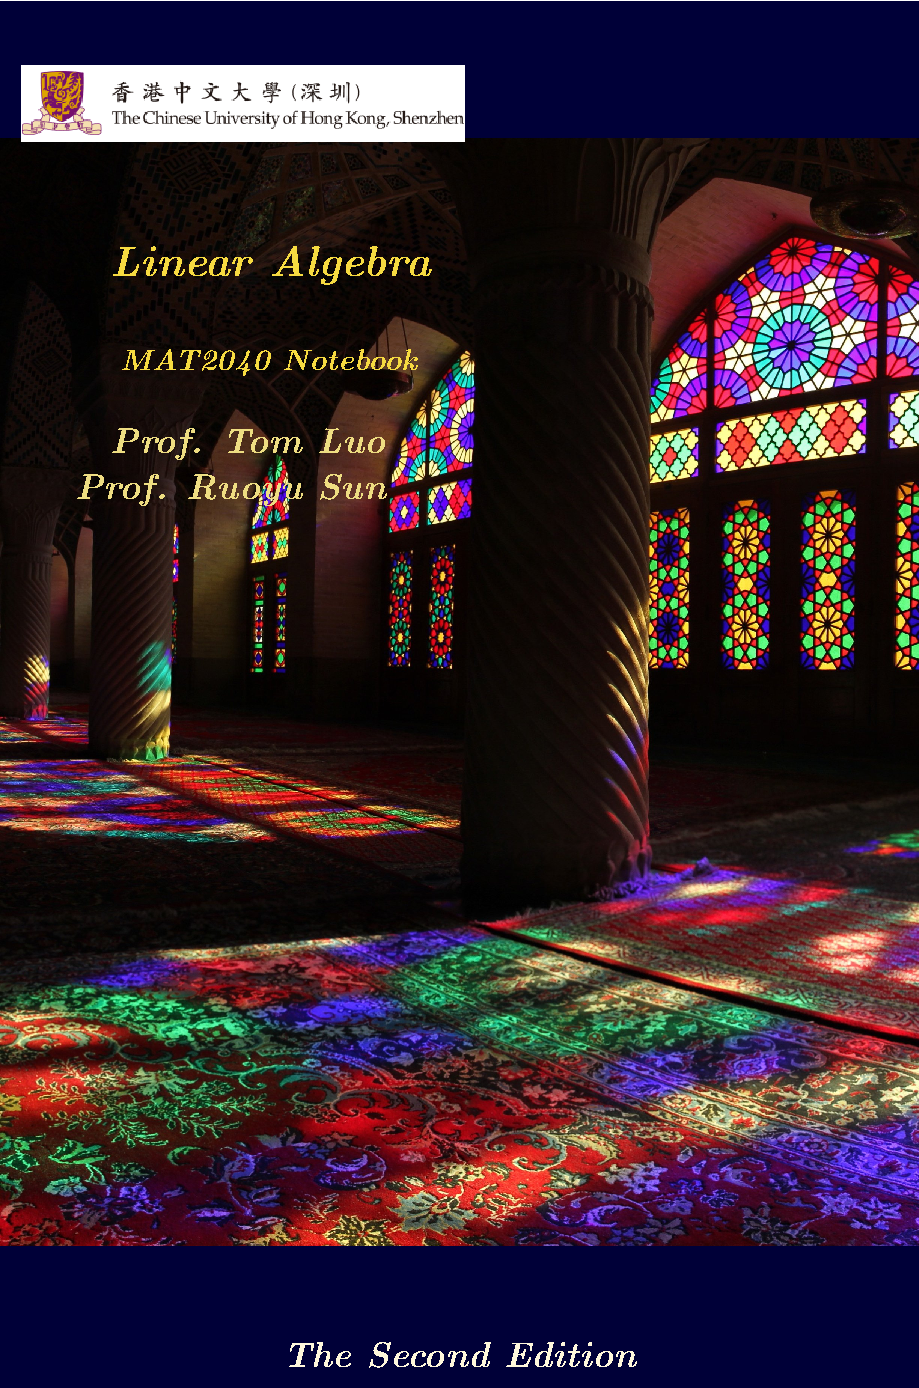
\includepdf[pages={1}]{book_cover/cover/FrontCover}
%%%%%%%%%%%%%%%%%%%%%%%%%%%%%%%%%%%%%%%%%%%%%%%%%%%%%%%%
%% Setting up title pages, type in the appropriate names here:

\booktitle{A First Course \\ In \\
Numerical Analysis}

\subtitle{MAT4001 Notebook}

\AuAff{Prof. Yutian Li\\ The Chinese University of Hongkong, Shenzhen}
%\AuAff{Prof. Ruoyu Sun\\ University of Illinois Urbana-Champaign}
%% \\ will start a new line.


%% Print Half Title and Title Page:
\halftitlepage
\titlepage

%%%%%%%%%%%%%%%%%%%%%%%%%%%%%%%%%%%%%%%%%%%%%%%%%%%%%%%%
%% Copyright Page
%\begin{copyrightpage}{year}
%Title, etc
%\end{copyrightpage}

% Note, you must use \ to start indented lines, ie,
% 
% \begin{copyrightpage}{2004}
% Survey Methodology / Robert M. Groves . . . [et al.].
% \       p. cm.---(Wiley series in survey methodology)
% \    ``Wiley-Interscience."
% \    Includes bibliographical references and index.
% \    ISBN 0-471-48348-6 (pbk.)
% \    1. Surveys---Methodology.  2. Social 
% \  sciences---Research---Statistical methods.  I. Groves, Robert M.  II. %
% Series.\\
%
% HA31.2.S873 2004
% 001.4'33---dc22                                             2004044064
% \end{copyrightpage}

%%%%%%%%%%%%%%%%%%%%%%%%%%%%%%%%%%%%%%%%%%%%%%%%%%%%%%%%
%% Only Dedication (optional) 
%\dedication{To my girlfriend Jianyu Yang}

\tableofcontents

%\listoffigures %optional
%\listoftables  %optional



% If your book has chapters written by different authors,
% you'll need a Contributors page.

% Use \begin{contributors}...\end{contributors} and
% then enter each author with the \name{} command, followed
% by the affiliation information.

% \begin{contributors}
% \name{Zhi-quan Luo,} Shenzhen Research Institute of Big Data, Lecturer
%
% \name{Ruoyu Sun,} Industrial and Enterprise Systems Engineering, Lecturer
%
% \name{Jie Wang,} The Chinese University of Hongkong, Shenzhen, Typer
% \end{contributors}

%%%%%%%%%%%%%%%%%%%%%%%%%%%%%%%%%%%%%%%%%%%%%%%%%%%%%%%%
% Optional Preface:
%\begin{preface}
%This book is intended for the foundation course MAT2040, which is the first course on the linear algebra. It aims to cover basic linear algebra knowledge and its simple applications. This book was first written in 2017, and it is reviewed and revised in 2018. We have corrected several mistakes shown in the previous book and modified some proofs a little bit to give readers better insights of linear algebra.  During the modification, we also refer to many reading materials, which are also recommended for you:
\begin{itemize}
\item
ENGG 5781 Course Notes by Prof. Wing-Kin (Ken) Ma,  CUHK, Hongkong, China,  http://www.ee.cuhk.edu.hk/$\sim$wkma/engg5781
\item
Roger A. Horn and Charles R. Johnson, Matrix Analysis (Second Edition), Cambridge University Press, 2012.
\item
S. Boyd and L. Vandenberghe, Introduction to Applied Linear Algebra (Vectors, Matrices, and Least Squares), Cambridge University Press, 2018.
\end{itemize}
The whole book can cover a semester course in a 14week, each section in which corresponds to a 2-hour lecture. If you read the whole book, and work some mini-exercises, you will learn a lot. We hope you will get the insights on linear algebra and apply them in your own subject.




%\prefaceauthor{}
%\where{CUHK(SZ)\\
% \today}
%\end{preface}
% ie,
% \begin{preface}
% This is an example preface.
% \prefaceauthor{R. K. Watts}
% \where{Durham, North Carolina\\
% September, 2004}

%%%%%%%%%%%%%%%%%%%%%%%%%%%%%%%%%%%%%%%%%%%%%%%%%%%%%%%%
% Optional Acknowledgments:

\acknowledgments
This book is from the MAT4001 in fall semester, 2018.
\authorinitials{CUHK(SZ)}  


%%%%%%%%%%%%%%%%%%%%%%%%%%%%%%%%%%%%%%%%%%%%%%%%%%%%%%%%
% Optional notations:
\begin{notations}
\acro{$\mathbb{R}^n$}{$n$-dimensional real space}
\acro{$\mathbb{C}^n$}{$n$-dimensional complex space}
\acro{$\mathbb{R}^{m\times n}$}{set of all $m\times n$ real-valued matrices}
\acro{$\mathbb{C}^{m\times n}$}{set of all $m\times n$ complex-valued matrices}
\acro{$x_i$}{$i$th entry of column vector $\bm x$}
\acro{$a_{ij}$}{$(i,j)$th entry of matrix $\bm A$}
\acro{$\bm a_i$}{$i$th column of matrix $\bm A$}
\acro{$\bm a_i\trans$}{$i$th row of matrix $\bm A$}
\acro{$\mathbb{S}^n$}{set of all $n\times n$ real symmetric matrices, i.e., $\bm A\in\mathbb{R}^{n\times n}$ and $a_{ij}=a_{ji}$ for all $i,j$}
\acro{$\mathbb{H}^n$}{set of all $n\times n$ complex Hermitian matrices, i.e., $\bm A\in\mathbb{C}^{n\times n}$ and $\bar{a}_{ij}=a_{ji}$ for all $i,j$}
\acro{$\bm A\trans$}{transpose of $\bm A$, i.e, $\bm B=\bm A\trans$ means $b_{ji}=a_{ij}$ for all $i,j$}
\acro{$\bm A\Her$}{Hermitian transpose of $\bm A$, i.e, $\bm B=\bm A\Her$ means $b_{ji}=\bar{a}_{ij}$ for all $i,j$}
\acro{$\trace(\bm A)$}{sum of diagonal entries of square matrix $\bm A$}
\acro{$\bm 1$}{A vector with all $1$ entries}
\acro{$\bm 0$}{either a vector of all
zeros, or a matrix of all zeros}
\acro{$\bm e_i$}{a unit vector with the nonzero element at the $i$th entry}
\acro{$\mathcal{C}(\bm A)$}{the column space of $\bm A$}
\acro{$\mathcal{R}(\bm A)$}{the row space of $\bm A$}
\acro{$\mathcal{N}(\bm A)$}{the null space of $\bm A$}
\acro{$\Proj_{\mathcal{M}}(\bm A)$}{the projection of $\bm A$ onto the set $\mathcal{M}$}
\end{notations}
\mainmatter
\setcounter{page}{1}

%%%%%%%%%%%%%%%%%%%%%%%%%%%%%%%%%%%%%%%%%%%%%%%%%%%%%%%%
% Optional introduction:
%\begin{introduction}
%
%The word \textit {traffic} becomes \textit {teletraffic} in telecommunications, as communications becomes telecommunications to indicate technology use, e.g., conversation from some distance through phones or Internet. The term teletraffic covers all kinds of computer communication traffic and telecom traffic.  This book includes teletraffic loss models.
%\end{introduction}

\chapter{Week2}
\section{Monday}\index{week2_Tuesday_lecture}
\subsection{Reviewing and Announments}
Tutorial: Thursday 7:00pm -9:00pm, ChengDao 208

Homework is due every Monday.

The first homework has been uploaded.

To proof the optimality condition in $\mathbb{R}^n$, we set $h(t) = f(x^*+td)$ for fixed $x^*$ and $d$. It follows that
\[
h'(t)=\nabla\trans f(x^*+td)d
\]
and
\[
h''(t)=d\trans\nabla^2f(x^*+td)d
\]
By the optimality condition for $\mathbb{R}$, we derive the necessary condition:
\[
\left\{
\begin{aligned}
\mbox{$h'(0)=\nabla\trans f(x^*)d=0$ for $\forall d$}\implies \mbox{$\nabla f(x^*)=0$;}\\
\mbox{$h''(0)=d\trans\nabla^2f(x^*)d=0$ for $\forall d$}
\implies
\mbox{$\nabla^2f(x^*)\succeq0$}
\end{aligned}
\right.
\]
together with the sufficient condition:
\[
\left\{
\begin{aligned}
\mbox{$\nabla f(x^*)=0$;}\\
\mbox{$\nabla^2f(x^*)\succ0$}
\end{aligned}
\right.
\]
\subsection{Quadratic Function Case Study}
Given a quadratic function 
\[
f(\bm x) =\frac{1}{2}\bm x\trans\bm Q\bm x+\bm b\trans\bm x
\]
w.l.o.g., assume the matrix $\bm Q$ is symmetric (recall the quadratic section studied in linear algebra).


\begin{definition}[Stationarity]
A point $\bm x^*$ is said to be the stationary point of $f(\bm x)$ if $\nabla f(\bm x^*)=\bm0$.
\end{definition}
To minimize such a function without constraint, we apply the optimality condition:
\begin{enumerate}
\item
The first order optimality condition is given by:
\[
\nabla f(\bm x) = \bm Q\bm x+\bm b=\bm0
\]
The stationary point of the quadratic function $f(\bm x)$ exists iff $\bm b\in\mathcal{C}(\bm Q).$
\item
The second order necessary condition should be:
\[
\nabla^2 f(\bm x)=\bm Q\succeq0
\]
\end{enumerate}
For this special case, if $\bm Q\succeq0$, then $f(\bm x)$ is convex, the solutions to $\nabla f(\bm x) =\bm0$ are local minimum points. Furthermore, they are global minimum points (prove by Taylor Expansion). However, for general functions, we cannot obtain such good results.

\paragraph{Least Squares Problem} Such a problem has been well-studied in statistics given by:
\[
\min_{\bm x}f(\bm x):=\frac{1}{2}\|\bm{Ax}-\bm b\|_2^2
\]
The first order derivative of the minimizer should satisfy:
\[
\nabla f(\bm x)=\bm A\trans(\bm A\bm x-\bm b)
\]
Note that $\bm A\trans\bm b\in\mathcal{C}(\bm A\trans\bm A)$, thus the least squares problem always has a solution. However, such a solution is not unique unless $\bm A$ is full rank.
\paragraph{A Non-trival Quadratic Function}
To minimize the function
\[
f(x,y)=\frac{1}{2}(\alpha x^2+\beta y^2)-x
\] 
We take the first order derivative to be zero:
\[
\nabla f(x,y)=\begin{bmatrix}
\alpha x-1\\\beta y
\end{bmatrix}=\bm0
\]
The second order derivative is given by:
\[
\nabla^2 f(x,y)=\begin{bmatrix}
\alpha&0\\0&\beta
\end{bmatrix}
\]
The optimal solutions depend on the value of $\alpha$ and $\beta$: (although we haven't introduce the definition for convex formally)
\begin{itemize}
\item
If $\alpha,\beta>0$, then this problem is \emph{strongly convex}. By the necessary and sufficient optimality condition for convex problem, we find that $(\frac{1}{\alpha},0)$ is the unique local minimum (It is also the global minimum by plotting the figure).
\item
If $\alpha=0$, this problem has no solution. The objective value $f(x,y)\to-\infty$ as $x\to
\infty$.
\item
If $\beta=0,\alpha>0$, this problem is convex.  By the necessary and sufficient optimality condition for convex problem, $\{(\frac{1}{\alpha},\xi)\mid \xi\in\mathbb{R}\}$ is the set of local minimum. (By plotting the graph, we find that such set is the set of global minimum points)
\item
For $\alpha>0,\beta<0$ case, this problem is non-convex. Actually, $f(x,y)\to-\infty$ as $y\to
\infty$. Hence, this problem has no global minimum point.
\end{itemize}

\paragraph{A Non-trival Function Study}
To minimize the function
\[
\begin{array}{ll}
\min&f(\bm y)=e^{y_1}+\cdots+e^{y_n}\\
\mbox{such that}&y_1+\cdots+y_n=S
\end{array}
\]
We can transform such a constrainted optimization problem into unconstrainted. Let $y_n=S-y_1-\cdots-y_{n-1}$ and substitute it into the objective function, it suffices to solve
\[
\min e^{y_1}+\cdots+e^{y_{n-1}}+e^{S-y_1-\cdots-y_{n-1}}
\]
The stationary point should satisfy:
\[
e^{y_i}=e^{S-y_1-\cdots-y_{n-1}},
\qquad
i=1,2,\dots,n-1
\]
Or equivalently, $y_1=y_2=\cdots=y_{n-1}=y_n$. Hence we derive the unique stationary point:
\[
y_1^*=y_2^*=\cdots=y_n^*=\frac{S}{n}
\]
The value on the stationary point is $f(y^*)=ne^{S/n}$. By checking the second order sufficient optimality condition,
\[
\frac{f}{\partial y_i\partial y_j}=\left\{
\begin{aligned}
e^{y_i}+e^{S-y_1-\cdots-y_{n-1}}&\quad i=j\\
e^{s-y_1-\cdots-y_{n-1}}&\quad i\ne j
\end{aligned}
\right.\implies
\nabla^2 f=e^{s-y_1-\cdots-y_{i-1}-y_i-y_{n-1}}\bm E
+\diag(e^{y_1},\dots,e^{y_{n-1}})
\]
where $\bm E$ is a matrix with entries all ones. Thus $\nabla^2 f\succ0$ for any stationary point. By the second order sufficient optimality condition, this stationary point is local minimum. Actually, for this special problem, this unique local minimum point is the global minimum.
\begin{remark}
In this problem, we find that this stationary point is the unique local minimum point, but the unique local minimum point is not necessarily the global minimum point, unless the function is \emph{coercive} or the feasible region is compact. Here is the counter-example: $f(x)=x^2-x^4$. We will discuss the definition for coercive in the future.
\end{remark}











\section{Thursday}\index{week5_Thursday_lecture}
\subsection{Orthogonality}
Recall that two vectors are orthogonal if their inner product is zero:
\[
\bm u\perp\bm v
\Longleftrightarrow
\inp{\bm u}{\bm v}=0
\]

Orthogonality among vectors has an important property:
\begin{proposition}
If \emph{nonzero} vectors $v_1,\dots,v_k$ are mutually orthogonal, i.e., $v_i\perp v_j$ for any $i\ne j$, then $\{v_1,\dots,v_k\}$ must be ind.
\end{proposition}
\begin{proof}
It suffices to show that 
\[
\alpha_1v_1+\dots+\alpha_kv_k=\bm 0 \implies
\alpha_i=0\text{ for any $i\in\{1,2,\dots,k\}$.}
\]
\begin{itemize}
\item
We do inner product to show $\alpha_1$ must be zero:
\[
\begin{aligned}
\inp{v_1}{\alpha_1v_1+\dots+\alpha_kv_k}
&=\inp{v_1}{\bm 0}=0\\
&=\alpha_1\inp{v_1}{v_1}+\alpha_2\inp{v_1}{v_2}+\dots+\alpha_k\inp{v_1}{v_k}\\
&=\alpha_1\inp{v_1}{v_1}=\alpha_1\|v_1\|_2^2\\
&=0
\end{aligned}
\]
Since $v_1\ne \bm 0$, we have $\alpha_1=0$.
\item
Similarly, we have $\alpha_i=0$ for $i=1,\dots,k$.
\end{itemize}
\end{proof}
Now we can also talk about orthogonality among spaces:
\begin{definition}[Subspace Orthogonality]
Two subspaces $\bm U$ and $\bm V$ of a vector space are \emph{orthogonal} if every vector $\bm u$ in $\bm U$ is \textit{perpendicular} to every vector $\bm v$ in $\bm V$:
\[
\begin{array}{lll}
\mbox{\emph{Orthogonal subspaces}}
&
\bm u\perp\bm v,
&
\forall\bm u\in\bm U,\bm v\in\bm V.
\end{array}
\]
\end{definition}
\begin{example}
Two walls look \textit{perpendicular} but they are not orthogonal subspaces! The meeting line is in both $\bm U$ and $\bm V$-and this line is not perpendicular to itself. Hence, two planes (both with dimension $2$ in $\mathbb{R}^{3}$) cannot be orthogonal subspaces.

\begin{figure}[H]
\centering
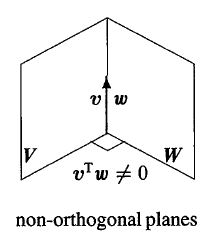
\includegraphics{week5/orthogonality}
\caption{Orthogonality is impossible when $\dim\bm U+\dim\bm V>\dim(\bm U\cup\bm V)$}
\end{figure}
\end{example}
\begin{remark}
When a vector is in two orthogonal subspaces, it \textit{must} be zero. It is \emph{perpendicular} to
itself. 
\\The reason is clear: this vector $\bm u\in\bm U$ and $\bm u\in\bm V$, so $\inp{\bm u}{\bm u}=0$. It has to be zero vector.
\end{remark}
If two subspaces are perpendicular, their basis must be ind.
\begin{theorem}
Assume $\{u_1,\dots,u_k\}$ is the basis for $\bm U$, $\{v_1,\dots,v_l\}$ is the basis for $\bm V.$ If $\bm U\perp\bm V$ ($u_i\perp v_j$ for $\forall i,j$), then $u_1,u_2,\dots,u_k,v_1,v_2,\dots,v_l$ must be ind.
\end{theorem}
\begin{proof}
Suppose there exists $\{\alpha_1,\dots,\alpha_k\}$ and $\{\beta_1,\dots,\beta_l\}$ such that
\[
\alpha_1u_1+\dots+\alpha_ku_k+\beta_1v_1+\dots+\beta_lv_l=\bm 0
\]
then equivalently,
\[
\alpha_1u_1+\dots+\alpha_ku_k=-(\beta_1v_1+\dots+\beta_lv_l).
\]
Then we set $\bm w=\alpha_1u_1+\dots+\alpha_ku_k$, obviously, $\bm w\in\bm U$ and $\bm w\in\bm V$.

 Hence it must be zero (This is due to remark above). Thus we have
\begin{gather*}
\alpha_1u_1+\dots+\alpha_ku_k=\bm 0\\
\beta_1v_1+\dots+\beta_lv_l=\bm 0.
\end{gather*}
Due to the independence, we have $\alpha_i=0$ and $\beta_j=0$ for $\forall i,j$. 
\end{proof}
\begin{corollary}
For subspaces $\bm U$ and $\bm V$, we obtain
\[
\dim(\bm U\cup\bm V)\le \dim(\bm U) + \dim(\bm V).
\]
\end{corollary}
For subspaces $\bm U$ and $\bm V\in\mathbb{R}^{n}$, if $\mathbb{R}^{n}=\bm U\cup\bm V$, and moreover, $n=\dim(\bm U)+\dim(\bm V)$, then we say $\bm V$ is the \emph{orthogonal complement} of $\bm U$.
\begin{definition}[orthogonal complement]
For subspaces $\bm U$ and $\bm V\in\mathbb{R}^{n}$, if $\dim(\bm U)+\dim(\bm V)=n$ and $\bm U\perp\bm V$, then we say $\bm V$ is the \emph{orthogonal complement} of $\bm U$. We denote $\bm V$ as $\bm U^{\perp}$.

Moreover, $\bm V=\bm U^{\perp}$ iff $\bm V^{\perp}=\bm U$.
\end{definition}
\begin{example}
Suppose $\bm U\cup\bm V=\mathbb{R}^{3}$, $\bm U=\Span\{\bm e_1,\bm e_2\}$. If $\bm V$ is the orthogonal complement of $\bm U$, then $\bm V=\Span\{\bm e_3\}$.
\end{example}

Next we study the relationship between the null space and the row space in $\mathbb{R}^n$.
\begin{theorem}[Fundamental theorem for linear alegbra, part 2] Given $\bm A\in\mathbb{R}^{m\times n}$,

\emph{$N(\bm A)$ is the orthogonal complement of the row space of $\bm A$, $\mathcal{C}(\bm A\trans)$ (in $\mathbb{R}^{n}$).}

\emph{$N(\bm A\trans)$ is the orthogonal complement of the column space $\mathcal{C}(\bm A)$ (in $\mathbb{R}^{m}$).}
\end{theorem}
\begin{proof}
\begin{itemize}
\item
Firstly, we show $\dim(N(\bm A))+\dim(\mathcal{C}(\bm A\trans))=n$:

We know that $\dim(N(\bm A))=n-r$ and $\dim(\mathcal{C}(\bm A\trans)) = r$, where $r=\rank(\bm A)$.

Hence $\dim(N(\bm A))+\dim(\mathcal{C}(\bm A\trans))=n$.
\item
Then we show $N(\bm A)\perp \mathcal{C}(\bm A\trans)$:

For any $x\in N(\bm A)$, if we set $\bm A=\begin{bmatrix}
a_1\trans\\a_2\trans\\\vdots\\a_m\trans
\end{bmatrix}$, then we obtain:
\[
\bm{Ax}=\begin{bmatrix}
a_1\trans\\a_2\trans\\\vdots\\a_m\trans
\end{bmatrix}\begin{bmatrix}
\bm x
\end{bmatrix}=\begin{bmatrix}
0\\0\\\vdots\\0
\end{bmatrix}
\]
Hence \textit{every row has a zero product with} $\bm x$, i.e., $\inp{a_i}{\bm x}=0$ for $\forall i\in\{1,2,\dots,m\}$.

For any $y=\sum_{i=1}^m\alpha_ia_i\in \mathcal{C}	(\bm A\trans)$, we obtain:
\[
\begin{aligned}
\inp{\bm x}{y}&=\inp{y}{\bm x}=\inp{\sum_{i=1}^m\alpha_ia_i}{\bm x}\\
&=\sum_{i=1}^{m}\alpha_i\inp{a_i}{\bm x}=0.
\end{aligned}
\]
Hence $\bm x\perp y$ for $\forall \bm x\in N(\bm A)$ and $y\in \mathcal{C}(\bm A\trans)$.\\
\end{itemize}
Hence $N(\bm A)^{\perp}=\mathcal{C}(\bm A\trans)$. Similarly, we have $N(\bm A\trans)^{\perp}=\mathcal{C}(\bm A)$. 
\end{proof}

\begin{corollary}
$\bm{Ax}=\bm b$ is solvable if and only if $\bm y\trans\bm A=\bm 0$ implies $\bm y\trans\bm b$=0.
\end{corollary}
\begin{proof} The following statements are equivalent:
\begin{itemize}
\item
$\bm{Ax}=\bm b$ is solvable.
\item
$\bm b\in \mathcal{C}(\bm A)$.
\item
$\bm b\in N(\bm A\trans)^{\perp}$
\item
$\bm y\trans\bm b=0$ for $\forall y\in N(\bm A\trans)$
\item
Given $\bm y\trans\bm A=\bm 0$, i.e., $y\in N(\bm A\trans)$, it implies $\bm y\trans\bm b=0$.
\end{itemize}
\end{proof}
The \emph{Inverse Negative Proposition} is more commonly useful:
\begin{corollary}
$\bm{Ax}=\bm b$ has no solution if and  and only if $\exists \bm y$ s.t. $\bm y\trans\bm A=0$ and $\bm y\trans\bm b\ne 0$.
\end{corollary}
We could extend this corollary into general case:
\begin{remark}
\begin{theorem}\label{theorem_12.3}
$\bm{Ax}\ge\bm b$ has no solution if and only if $\exists \bm y\ge\bm 0$ such that $\bm y\trans\bm A=\bm 0$ and $\bm y\trans\bm b\ge \bm 0$.
\end{theorem}
$\bm y\trans\bm A=0$ requires that there exists one linear combination of the row space to be zero.

The complete proof for this theorem is not required in this course. We only show the necessity case.
\begin{proof}[Necessity case.]
Suppose $\exists \bm y\ge\bm 0$ such that $\bm y\trans\bm A=\bm 0$ and $\bm y\trans\bm b\ge \bm 0$. Assume there exists $x^{*}$ such that $\bm Ax^{*}\ge\bm b$. By postmultiplying $\bm y\trans$ we have 
\[\bm y\trans\bm Ax^{*}\ge\bm y\trans\bm b>\bm 0
\implies 
\bm 0>\bm 0.
\]
which is a contradiction!
\end{proof}
\end{remark}

\begin{example}
Given the system 
\begin{align}
x_1+x_2&\ge1\label{Eq:6:3}
\\
-x_1&\ge-1\label{Eq:6:4}
\\
-x_2&\ge2\label{Eq:6:5}
\end{align}
Eq.(\ref{Eq:6:3})$\x$1+Eq(\ref{Eq:6:4})$\x$1+Eq.(\ref{Eq:6:5})$\x$1 gives
\[
0\ge 2
\]
which is a contradiction!\\
So the key idea of theorem (\ref{theorem_12.3}) is to construct a linear combination of row space to let it become zero. If the right hand is larger than zero, then this system has no solution.
\end{example}
\begin{remark}
\begin{corollary}
If $\bm A=\bm A\trans$, then $N(\bm A\trans)^{\perp}=\mathcal{C}(A)=\mathcal{C}(\bm A\trans)=N(\bm A)$.
\end{corollary}
\begin{corollary}\label{corollary_12.5}
The system $\bm{Ax}=\bm b$ may not have a solution, but $\bm A\trans\bm A\bm x=\bm A\trans\bm b$ always have at least one solution for $\forall\bm b$.
\end{corollary}
\begin{proof}
Since $\bm A\trans\bm A$ is symmetric, we have $\mathcal{C}(\bm A\trans\bm A)=\mathcal{C}(\bm A\bm A\trans)$. Show by yourself that $\mathcal{C}(\bm A\bm A\trans)=\mathcal{C}(\bm A\trans)$, hence $\mathcal{C}(\bm A\trans\bm A)=\mathcal{C}(\bm A\trans)$.

For any vector $\bm b$, we have $\bm A\trans\bm b\in \mathcal{C}(\bm A\trans)\implies\bm A\trans\bm b\in \mathcal{C}(\bm A\trans\bm A)$, which means there exists a linear combination of the columns of $\bm A\trans\bm A$ that equals to $\bm b$.

Or equivalently, there exists a solution to $\bm A\trans\bm A\bm x=\bm A\trans\bm b$.
\end{proof}
\begin{corollary}\label{corollary_12.6}
$\bm A\trans\bm A$ is invertible if and only if $\bm A$ is full column rank, i.e., columns of $\bm A$ are ind.
\end{corollary}
\begin{proof}
We have shown that $C(\bm A\trans\bm A)=C(\bm A\trans)$.

Hence $C(\bm A\trans\bm A)^{\perp}=C(\bm A\trans)^{\perp}\implies N(\bm A\trans\bm A)=N(\bm A)$.

Thus, the following statements are equivalent:
\begin{itemize}
\item
$\bm A$ has ind. columns
\item
$N(\bm A)=\{\bm 0\}$
\item
$N(\bm A\trans\bm A)=\{\bm 0\}$
\item
$\bm A\trans\bm A$ is invertible.
\end{itemize}
\end{proof}
\end{remark}
\subsection{Least Squares Approximations}
The linear system $\bm{Ax}=\bm b$ often has no solution, if so, what should we do?

We cannot always get the error $\bm e=\bm b-\bm{Ax}$ down to zero, so we want to use \textit{least square method} to minimize the error. In other words, our goal is to
\[
\min_{\bm x\in\mathbb{R}^n}\bm e^2:=\min_{\bm x}\|\bm{Ax}-\bm b\|^2=\sum_{i=1}^{m}(a_i\trans\bm x-b_i)^2
\]
where $\bm A\in\mathbb{R}^{m\times n}$ and $\bm b\in\mathbb{R}^m$. The minimizer $\bm x$ is called the \emph{linear least squares solution}.

\subsubsection{Least Squares by Convex Optimization}
Firstly, you should know some basic calculus knowledge for matrix:
\paragraph{The Chian Rule} Given two vectors $f(x),g(x)$ of appropriate size,
\[
\frac{\partial(f\trans g)}{\partial x}=\frac{\partial f(x)}{\partial x}g(x)+\frac{\partial g(x)}{\partial x}f(x)
\]
\paragraph{Examples of Matrix Derivative}
\begin{align}
\frac{\partial(a\trans \bm x)}{\partial \bm x}&=a\\
\frac{\partial(a\trans \bm A\bm x)}{\partial \bm x}&=\frac{\partial((\bm A\trans a)\trans\bm x)}{\partial \bm x}=\bm A\trans a\\
\frac{\partial(\bm A\bm x)}{\partial \bm x}&=\bm A\trans\\
\frac{\partial(\bm x\trans\bm A\bm x)}{\partial \bm x}&=\bm A\bm x+\bm A\trans\bm x
\end{align}

Thus, in order to minimize $\|\bm{Ax}-\bm b\|^2=(\bm{Ax}-\bm b)\trans(\bm{Ax}-\bm b)$, it suffices to let its \emph{derivative} with respect to $\bm x$ to be \emph{zero.} (Since $\|\bm{Ax}-\bm b\|^2$ is convex, which will be discussed in detail in other courses.) Hence we have:
\[\begin{aligned}
\frac{\partial (\bm{Ax}-\bm b)\trans(\bm{Ax}-\bm b)}{\partial \bm x}&=\frac{\partial(\bm{Ax}-\bm b)}{\partial \bm x}(\bm{Ax}-\bm b)+\frac{\partial(\bm{Ax}-\bm b)}{\partial \bm x}(\bm{Ax}-\bm b)\\
&=2\frac{\partial(\bm{Ax}-\bm b)}{\partial \bm x}(\bm{Ax}-\bm b)\\
&=2(\frac{\partial(\bm A\bm x)}{\partial \bm x}-\frac{\partial(\bm b)}{\partial \bm x})(\bm{Ax}-\bm b)\\
&=2\bm A\trans(\bm{Ax}-\bm b)=\bm 0.
\end{aligned}
\]
Or equivalently, 
\[
\bm A\trans\bm{Ax}=\bm A\trans\bm b.
\]
According to corollary (\ref{corollary_12.5}), this equation always exists a solution. This equation is called the \emph{normal equation}.
\begin{theorem}\label{theorem_12.4}
A vector $\bm x_{\text{LS}}$ is an optimal solution to the least squares problem
\begin{subequations}
\begin{equation}
\min_{\bm x\in\mathbb{R}^n}\|\bm b-\bm{Ax}\|_2^2
\end{equation}
if and only if it satisfies
\begin{equation}
\bm A\trans\bm A\bm x_{\text{LS}} = \bm A\trans\bm b.
\end{equation}
\end{subequations}
\end{theorem}
\subsubsection{Fit a stright line}
Given a collection of data $(\bm x_i,y_i)$ for $i=1,\dots,m$, we can use a stright line to fit these points:
\[
\left\{
\begin{aligned}
y_1&=a_0+a_1x_{1,1}+a_2x_{1,2}+\dots+a_nx_{1,n}+\varepsilon_1\\
y_2&=a_0+a_1x_{2,1}+a_2x_{2,2}+\dots+a_nx_{2,n}+\varepsilon_2\\
\vdots\\
y_m&=a_0+a_1x_{m,1}+a_2x_{m,2}+\dots+a_nx_{m,n}+\varepsilon_m
\end{aligned}
\right.
\]
Our fit line is 
\[
\hat y=a_0+a_1x_1+a_2x_2+\dots+a_nx_n
\]
In \textit{compact matrix form}, we have
\[
\begin{bmatrix}
y_1\\y_2\\\vdots\\y_n
\end{bmatrix}
=\begin{bmatrix}
1&x_{1,1}&x_{1,2}&\dots&x_{1,n}\\
1&x_{2,1}&x_{2,2}&\dots&x_{2,n}\\
\vdots&\vdots&&&\\
1&x_{m,1}&x_{m,2}&\dots&x_{m,n}\\
\end{bmatrix}\begin{bmatrix}
a_0\\a_1\\a_2\\\vdots\\a_{n}
\end{bmatrix}+\begin{bmatrix}
\varepsilon_1\\\varepsilon_2\\\vdots\\\varepsilon_m
\end{bmatrix}
\]
Or equivalently, we have 
\[
\bm y=\bm{Ax}+\bm \varepsilon
\]
where $\bm A =\begin{bmatrix}
1&x_{1,1}&x_{1,2}&\dots&x_{1,n}\\
1&x_{2,1}&x_{2,2}&\dots&x_{2,n}\\
\vdots&\vdots&&&\\
1&x_{m,1}&x_{m,2}&\dots&x_{m,n}\\
\end{bmatrix}_{m\times (n+1)}$, $\bm x=\begin{bmatrix}
a_0\\a_1\\a_2\\\vdots\\a_{n}
\end{bmatrix}_{(n+1)\times 1}$, $\bm \varepsilon=\begin{bmatrix}
\varepsilon_1\\\varepsilon_2\\\vdots\\\varepsilon_m
\end{bmatrix}_{m\times 1}$.\\
Our goal is to minimize $\|\hat{\bm y}-\bm y\|^2=\|\bm{Ax}-\bm y\|^2$. Then by theorem (\ref{theorem_12.4}), it suffices to sovle $\bm A\trans\bm A\bm x=\bm A\trans\bm y$.

\subsection{Projections}
In corollary (\ref{corollary_12.6}), we know that if $\bm A$ has ind. columns, then $\bm A\trans\bm A$ is invertible. On this condition, the normal equation $\bm A\trans\bm A\bm x=\bm A\trans\bm b$ has the unique solution $\bm x^{*}=(\bm A\trans\bm A)^{-1}\bm A\trans\bm b$, which follows that the error $\bm b-\bm A\bm x^{*}$ is minimized. Note that $\bm A\bm x^{*}=\bm A(\bm A\trans\bm A)^{-1}\bm A\trans\bm b$ is \emph{approximately} equal to $\bm b$. 
\begin{itemize}
\item
If $\bm b$ and $\bm{A}\bm x^{*}$ are exactly in the same space, i.e., $\bm b\in\mathcal{C}(\bm A)$, then $\bm{A}\bm x^{*}=\bm b$. The error is equal to zero.
\item
Otherwise, just as the Figure (\ref{figure_12.2}) shown, $\bm A\bm x^{*}$ is the projection of $\bm b$ to subspace $\mathcal{C}(\bm A)$.
\end{itemize}
\begin{figure}[t]
\centering
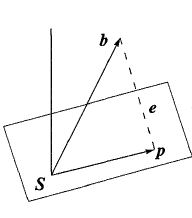
\includegraphics{week5/projection}
\caption{The projection of $\bm b$ onto a subspace $\bm S:=\mathcal{C}(\bm A)$.}\label{figure_12.2}
\end{figure}
\begin{definition}[Projection]
Let $\bm S\in\mathbb{R}^{m}$ be a non-empty closed set and $\bm b\in\mathbb{R}^m$ be given. Then the projection of $\bm b$ onto the set $\bm S$ is the solution to
\[
\min_{\bm z\in\bm S}\|\bm z-\bm b\|_2^2,
\]
where we use notation $\Proj_{\bm S}(\bm b)$ to denote the projection of $\bm b$ onto $\bm S$.
\end{definition}
By definition, the projection of $\bm b$ onto the subspace $\mathcal{C}(\bm A)$ is given by 
\[
\Proj_{\mathcal{C}(\bm A)}(\bm b):=\bm A\bm x^*,\quad
\text{where }\bm x^*=\arg\min_{\bm x\in\mathbb{R}^n}\|\bm{Ax} - \bm b\|.
\]

\begin{definition}[Projection matrix]
Given the projection
\[
\Proj_{C(\bm A)}(\bm b):=\bm A\bm x^{*}=\bm A(\bm A\trans\bm A)^{-1}\bm A\trans\bm b,
\]
since $[\bm A(\bm A\trans\bm A)^{-1}\bm A\trans]\bm b$,
we call the projection operator $\bm P:=\bm A(\bm A\trans\bm A)^{-1}\bm A\trans$ as the \emph{projection matrix} of $\bm A$.
\end{definition}
\begin{definition}[Idempotent]
Let $\bm A$ be a \emph{square} matrix that satisfies $\bm A=\bm A\bm A$, then $\bm A$ is called an \emph{idempotent} matrix.
\end{definition}
Let's show that the projection matrix is \textit{idempotent}:
\[
\begin{aligned}
\bm P^{2}&=\bm A(\bm A\trans\bm A)^{-1}\bm A\trans\bm A(\bm A\trans\bm A)^{-1}\bm A\trans\\
&=\bm A(\bm A\trans\bm A)^{-1}(\bm A\trans\bm A)(\bm A\trans\bm A)^{-1}\bm A\trans\\
&=\bm A(\bm A\trans\bm A)^{-1}\bm A\trans=\bm P.
\end{aligned}
\]

\subsubsection{Observations}
\begin{itemize}
\item
Suppose $\bm b\in \mathcal{C}(\bm A)$, i.e., $\exists \bm x$ s.t. $\bm{Ax}=\bm b$. Then the projection of $\bm b$ is exactly $\bm b$:
\[
\begin{aligned}
\bm{Pb}&=\bm A(\bm A\trans\bm A)^{-1}\bm A\trans(\bm b)\\
&=\bm A(\bm A\trans\bm A)^{-1}\bm A\trans(\bm{Ax})\\
&=\bm A(\bm A\trans\bm A)^{-1}(\bm A\trans\bm A)\bm x\\
&=\bm{Ax}=\bm b.
\end{aligned}
\]
\item
Assume $\bm A$ has only one column, say, $\bm a$. Then we have
\[\begin{aligned}
\bm x^{*}&=(\bm A\trans\bm A)^{-1}\bm A\trans\bm b=\frac{\bm a\trans\bm b}{\bm a\trans\bm a}\\
\bm A\bm x^{*}&=\bm{Pb}=\bm A(\bm A\trans\bm A)^{-1}\bm A\trans(\bm b)=\frac{\bm a\trans\bm b}{\bm a\trans\bm a}\times\bm a=\frac{\bm a\trans\bm b}{\|\bm a\|^2}\times\bm a
\end{aligned}
\]
More interestingly, 
\[\frac{\bm a\trans\bm b}{\|\bm a\|^2}\times\bm a=\frac{\|\bm a\|\|\bm b\|\cos\theta}{\|\bm a\|^2}\times\bm a=\|\bm b\|\cos\theta\times\frac{\bm a}{\|\bm a\|}\]
which is the projection of $\bm b$ onto a line $\Span\{\bm a\}$. (Shown in figure (\ref{Fig:6:3}).)
\begin{figure}[H]
\centering
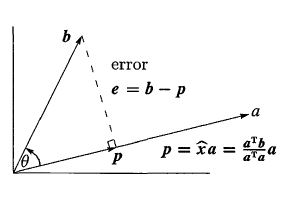
\includegraphics[width=10cm]{week5/projection_line}
\caption{The projection of $\bm b$ onto a line $\bm a$.}
\label{Fig:6:3}
\end{figure}
More generally, we can write the projection of $\bm b$ onto the line $\Span\{\bm a\}$ as:
\[
\Proj_{\Span\{\bm a\}}(\bm b)=\frac{\inp{\bm a}{\bm b}}{\inp{\bm a}{\bm a}}\bm a
\]
\paragraph{Changing an Orthogonal Basis}
Note that the error $\bm b-\Proj_{\Span\{\bm a\}}(\bm b)$ is perpendicular to $\bm a$, and $\bm b-\Proj_{\Span\{\bm a\}}(\bm b)\in\Span\{\bm a,\bm b\}.$

If we define $\bm b'=\bm b-\Proj_{\Span\{\bm a\}}(\bm b)$, then it's easy to check that $\Span\{\bm a,\bm b'\}=\Span\{\bm a,\bm b\}$ and $\bm a\perp\bm b'$. 

Hence, we convert the basis $\{\bm a,\bm b\}$ into another basis $\{\bm a,\bm b'\}$ such that the elements are orthogonal to each other. For general subspace we could also use this approach to obtain an orthogonal basis, which will be discussed in next lecture. 
\end{itemize}









%\section{Friday}\index{week7_Thursday_lecture}

\subsection{Polynomials}
\begin{definition}[polynomial]
Let $k$ be a field, and $f=\sum_{i=0}^nc_ix^i$ be a polynomial in $k[x]$. An element $a\in k$ is a root of $f$ if
\[
f(a)=\sum_{i=0}^nc_ia^i=0
\]
in $k$.
\end{definition}
question: what is $k[x]$?
\begin{corollary}
For all $f\in k[x]$, $a\in k$, then there exists $q\in k[x]$ such that
\[
f=q(x-a)+f(a)
\]
\end{corollary}
\begin{proof}
By division theorem, there exists $q,r\in k[x]$ such that
\[
f=q\cdot (x-a)+r,\quad
\mbox{deg}r<\mbox{deg}(x-a)=1
\]
which implies $r$ is a constant. Evaluate both sides for $x=a$, we have
\[
f(a)=r.
\]
\end{proof}
\begin{proposition}[root theorem]
Let $k$ be a field, $f$ a polynomial is $k[x]$. Then $a\in k$ is a root of $f$ iff $(x-a)$ divides $f$ in $k[x]$.
\end{proposition}
\begin{proof}
For forward direction, there exists $q\in k[x]$ such that
\[
f=q(x-a)+f(a)=q(x-a)\implies (x-a)|f
\]
For the reverse direction, if $f=q(x-a)$ for some $q\in k[x]$, then $f(a)=q(a)(a-a)=0$, i.e., $a$ is a root of $f$.
\end{proof}
\begin{theorem}
Let $k$ be a field, $f$ a nonzero polynomial in $k[x]$
\begin{enumerate}
\item
If $f$ has some degree $n$, then it has at most $n$ roots in $k$
\item
If $f$ has degree $n$ and $a_1,\dots,a_n\in k$ are distinct roots of $f$, then
\[
f=c\prod_{i=1}^n(x-a_i)
\]
for some $c\in k$.
\end{enumerate}
\end{theorem}
\begin{proof}
\begin{enumerate}
\item
We show the first part by induction. Suppose it holds for all nonzero polynomails with degree strictly less than $n$, and $\mbox{deg}f=n$. If $f$ has no roots in $k$, the proof is complete, otherwise suppose a root $a\in k$. There exists $q\in k[x]$ such that
\[
f=q(x-a)
\]
For the any other root $b\in k$, we have 
\[
0=q(b)(b-a)
\]
Since $k$ is a firld, it has no zero divisors, which implies $q(b)=0$, since $b-a\ne0$. Thus $b$ is a root of $q$. Since $\mbox{deg}q<n$, by induction we imply $q$ has at most $n-1$ roots, i.e., $f$ has at most $n-1$ roots that are different from $a$.
\item
If $n=1$, then $f=c_0+c_1x$ for some $c_i\in k$ with $c_1\ne0$, which implies
\[
0=f(a_1)=c_0+c_1a_1\implies c_0=-c_1a_1\implies
f=-c_1a_1+c_1x=c_1(x-a_1)
\]
Suppose $n>1$, and the claim holds for all $n'\in\mathbb{N}$ such that $n'<n$. By previuos claim, there exists $q\in k[x]$ such that
\[
f=q(x-a_n)
\]
Since $\mbox{deg}q=n-1$, and for $1\le i<n$, we have
\[
0=f(a_i)=q(a_i)(a_i-a_n)\implies q(a_i=0),
\]
which implies $a_1,\dots,a_{n-1}$ are $n-1$ distinct roots of $q$ as well. Thus there exists $c\in k$ s.t.
\[
q=c(x-a_1)\cdots(x-a_{n-1}),
\]
which follows that
\[
f=q(x-a_n)=c(x-a_1)\cdots(x-a_n)
\]
\end{enumerate}
\end{proof}

\begin{corollary}
Let $k$ be a field. Let $f,g$ be nonzero polynomails in $k[x]$. Let $n=\max\{\mbox{deg}f,\mbox{deg}g\}$. If $f(a)=g(a)$ for $n+1$ distinct $a\in k$, then $f=g$.
\end{corollary}
\begin{proof}
Let $h=f-g$, then $\mbox{deg}h\le n$. There are $n+1$ distinct elements $a\in k$ s.t. $h(a)=0$. If $h\ne0$, then it is a nonzero polynomial of degree $\le n$ which has $n+1$ distinct roots, which is a constraction. $h=0$ implies $f=g$.
\end{proof}
\begin{definition}
A polynomail in $k[x]$ is called a \emph{monic polynomial} if its leading coefficient is $1$.
\end{definition}
\begin{theorem}
Let $k$ be a field, then the ring $k[x]$ is a PID.
\end{theorem}
\begin{corollary}
Let $k$ be a field, and $f,g$ be nonzero polynomials in $k[x]$. There exists a unique monic polynomial $d\in k[x]$ with the following properties:
\begin{enumerate}
\item
$(f,g)=(d)$
\item
$d$ divides both $f$ and $g$, i.e., there exists $a,b\in k[x]$ s.t. $f=ad,g=bd$
\item
There are polynomials $p,q\in k[x]$ such that $d=pf+qg$
\item
If $h\in k[x]$ is a divisor of $f,g$, then $h$ divides $d$.	
\end{enumerate}
This $d\in k[x]$ is called the \emph{greatest common divisor} (GCD) of $f$ and $g$. We say $f$ and $g$ are \emph{relatively prime} if their GCD is 1.
\end{corollary}
\begin{proof}
By the PID theorem, there exists $d=\sum_{n=0}^\infty a_ix^i\in k[x]$ such that $(d)=(f,g)$. Replacing $d$ with $a_n^{-1}d$, we assume $d$ is a monic polynomial. It remains to show that $d$ is unique. 

Suppose $(d)=(d')$, there exists nonzero $p,q\in k[x]$ such that
\[
d'=pd,\quad
d=qd'
\]
which follows that
\[
\mbox{deg}d'=\mbox{deg}d+\mbox{deg}p,\quad
\mbox{deg}d=\mbox{deg}q+\mbox{deg}d'=\mbox{deg}q+\mbox{deg}d+\mbox{deg}p,
\]
i.e., $\mbox{deg}p=\mbox{deg}q=0$. Thus $\mbox{deg}d=\mbox{deg}d'$. Comparing the leading coefficients of $d'$ and $pd$, we have $p=1$, i.e., $d=d'$.

The remaining part follows similarly.
\end{proof}
\begin{definition}[Irreducible]
Let $R$ be a commutative ring. A non-zero element $p\in R$ which is not a unit is said to be \emph{irreducible} if $p=ab$ implies that either $a$ or $b$ is a unit.
\end{definition}
\begin{example}
The set of irreducible elements in the ring $\mathbb{Z}$ is
\[
\{\pm p\mid p\mbox{ is a prime number}\}
\]
\end{example}
Let $k$ be a field.
\begin{proposition}
A polynomial $f\in k[x]$ is a unit iff it is a \emph{nonzero} constant polynomial.
\end{proposition}
\begin{proposition}
A nonzero nonconstant polynoimial $p\in k[x]$ is \emph{irreducible} iff there is no $f,g\in k[x]$ with $\mbox{deg}f,\mbox{deg}g<\mbox{deg}p$, such that $fg=p$.
\end{proposition}
\begin{proof}
\begin{enumerate}
\item
Suppose $p$ is irreducible, and $p=fg$ for some $f,g\in k[x]$ such that $\mbox{deg}f,\mbox{deg}g<\mbox{deg}p$. Then $p=fg$ implies that $\mbox{deg}f,\mbox{deg}g$ are both positive. By previous lemma, both $f,g$ are non-units, which is a contradiction.
\item
Conversely, suppose $p$ is a nonzero non-unit in $k[x]$, which is not equal to $fg$ for $\forall f,g\in k[x]$ with $\mbox{deg}f,\mbox{deg}g<\mbox{deg}p$. Then $p=ab$ for $a,b\in k[x]$ implies that either $a$ or $b$ must have the same degree as $p$, and the otehr factor must be a nonzero constant, i.e., a unit in $k[x]$. Thus $p$ is irreducible.
\end{enumerate}
\end{proof}

\begin{proposition}[Euclid's Lemma]
Let $k$ be a field. Let $f,g$ be polynomials in $k[x]$. Let $p$ be an irreducible polynomial in $k[x]$. If $p|fg$ in $k[x]$, then $p|f$ or $p|g$.
\end{proposition}
\begin{proof}
Suppose $p$ not divides $f$, then any \emph{common divisor} of $p$ and $f$ must have degree strictly less than $\mbox{deg}p$. Since $p$ is irreducible, this implies that any common divisor of $p$ and $f$ is a nonzero constant. Thus the GCD of $p$ and $f$ is 1. There exists $a,b\in k[x]$ such that
\[
ap+bf=1\implies
apg+bfg=g
\]
Since $p$ divides the LHS, it also divides the RHS.
\end{proof}
\begin{proposition}
If $f,g\in k[x]$ are relatively prime, and both divide $h\in k[x]$, then $fg|h$.
\end{proposition}
question
\begin{theorem}[Unique Factorization]
Let $k$ be a field. Every non-constant polynomial $f\in k[x]$ may be written as
\[
f=cp_1\cdots p_n
\]
where $c$ is a non-zero constant, and each $p_i$ is a monic irreducible polynomials in $k[x]$. The factorization is \emph{unique} up to the ordering of the factors.
\end{theorem}
\begin{proof}
Similar to the proof of unique factorization for $\mathbb{Z}$
\end{proof}
\begin{theorem}
Let $k$ be a field, $p$ be a polynomial in $k[x]$. The following statements are equivalent:
\begin{enumerate}
\item
$k[x]/(p)$ is a field
\item
$k[x]/(p)$ is an integral domain
\item
$p$ is irreducible in $k[x]$.
\end{enumerate}
\end{theorem}
\begin{proof}
\begin{enumerate}
\item
(2) implies (3): If $p$ is not irreducible, then there exists $f,g\in k[x]$ with degree strictly less than that of $p$, such that $p=fg$.

It's clear that $p$ does not divide $f$ or $g$ in $k[x]$. The equivalence classes $\bar f$ and $\bar g$ of $f$ and $g$, respectively, modulo $(p)$ is not equal to zero in $k[x]/(p)$. (question) On the other hand, $\bar f\cdot\bar g=\bar{fg}=\bar p=0$ in $k[x]/(p)$, which implies that $k[x]/(p)$ is not an integral domain, which is a contradction.
\item
(3) implies (1): By definiton, the multiplicative identity $1$ of a field is different from addictive identity $0$. We first check that the equivalence lcass $1\in k[x]$ in $k[x]/(p)$ is not zero. Since $p$ is irreducible, we have $\mbox{deg}p>0$, and $1\notin(p)$. Therefore $1+(p)\ne 0+(p)$ in $k[x]/(p)$.

Next, we need to show the existence of multiplicative inverse of any nonzero element in $k[x]/(p)$. Given any $f\in k[x]$ whose equivalence $\bar f$ modulo $(p)$ is nonzero in $k[x]/(p)$, we want to constracut $\bar{f}^{-1}$. Since $\bar{f}\ne0$ in $k[x]/(p)$, we have $f-0\notin(p)$, i.e., $p$ does not divide $f$. Since $p$ is irreducible, we have $gcd(p,f)=1$. There exists $g,h\in k[x]$ such that $fg+hp=1$. Thus $\bar{f}^{-1}=\bar{g}$. This is becasue $fg-1=hp$ implies $fg-1\in(p)$, i.e., $\bar{f}\bar{g}=\bar{fg}=1$ in $k[x]/(p)$.


\end{enumerate}
\end{proof}
\subsection{Polynomials over $\mathbb{Z}$ and $\mathbb{Q}$}
\begin{theorem}
Let $f=a_0+a_1x+\cdots+a_nx^n$ be a polynomial in $\mathbb{Q}[x]$, with $a_i\in\mathbb{Z}$. Every rational root $r$ of $f$ in $\mathbb{Q}$ has the form $r=b/c$ $(b,c\in\mathbb{Z})$, where $b|a_0$ and $c|a_n$
\end{theorem}
\begin{proof}
Let $r=b/c$ be a rational root of $f$, where $b,c$ are relatively prime integers. We have
\[
0=\sum_{i=1}^na_i(b/c)^i
\]
Multiplying both sides above equation by $c^n$, we have
\[
0=a_0c^n+a_1c^{n-1}b+\cdots+a_nb^n
\]
or equivalently,
\[
a_0c^n=-(a_1c^{n-1}+\cdots+a_nb^n)
\]
Since $b$ divides the RHS, and $b,c$ are relatively prime, $b$ must divide $a_0$. Similarly,
\[
a_nb^n=-(a_0c^n+\cdots+a_{n-1}cb^{n-1})
\]
It is clear that $c$ divides $a_n$.
\end{proof}
\begin{definition}
A polynomial $f\in\mathbb{Z}[x]$ is said to be \emph{primitive} if the gcd of its coefficients is 1.
\end{definition}
\begin{remark}
Note that if $f$ is monic, i.e., its leading coefficient is 1, then it is primitive. If $d$ is the gcd of the coefficients of $f$, then $\frac{1}{d}f$ is a primitive polynomial in $\mathbb{Z}[x]$.
\end{remark}
\begin{theorem}[Gauss's Lemma]
If $f,g$ are both primitive, then $fg$ is primitive.
\end{theorem}
\begin{proof}
Write $f=\sum_{k=0}^ma_kx^k$ and $g=\sum_{k=0}^nb_kx^k$, then $fg=\sum_{k=0}^{m+n}c_kx^k$, where
\[
c_{k}=\sum_{i+j=k}a_ib_j.
\]
Assume that $fg$ is not primitive, then there exists a prime $p$ such that $p$ divides $c_k$ for $k=0,1,\dots,m+n$. Since $f$ is primitive, there exists smallest $u$ s.t. $a_u$ is not dividible by $p$; similarly, a smallest $v$ s.t. $b_v$ is not divisible by $p$. We have
\[
c_{u+v}=\left(\sum_{i+j=u+v,(i,j)\ne(u,v)}a_ib_j\right)+a_ub_v,
\]
which implies that
\[
a_ub_v=c_{u+v}-
\left(\sum_{i+j=u+v,i<u}a_ib_j\right)
-
\left(\sum_{i+j=u+v,i>u}a_ib_j\right)
\]
By the minimum conditons on $u$ and $v$, each term on the RHS of the above equation is divisible by $p$. Thus $p$ divides $a_u$ and $b_v$, which implies that $p$ divides either $a_u$ or $b_v$, which is a contradiction.
\end{proof}
\begin{proposition}
Every nonzero $f\in\mathbb{Q}[x]$ has a unique factorization:
\[
f=c(f)f_0,
\]
where $c(f)$ is a positive rational number, and $f_0$ is a primitive polynomial in $\mathbb{Z}[x]$.
\end{proposition}
\begin{definition}
The rational number $c(f)$ is called the \emph{content} of $f$.
\end{definition}















%\section{Assignment One}\index{Assignment One}
\begin{enumerate}
\item
Consider the system
\begin{align*}
ax+2y+3z&=b_1\\
ax+ay+4z&=b_2\\
ax+ay+az&=b_3\\
\end{align*}
For what three values of $a$ will the \textit{elimination} fail to give the pivots? (\textit{Pivots means the first nonzero entry on rows.})
\item
It is impossible for a system of linear equations to have \textit{exactly} two solutions? Explain your answers. And you may consider the following questions as intuitions to derive your final solution.
\begin{enumerate}
\item
In $\mathbb{R}^3$ if $(x,y,z)$ and $(X,Y,Z)$ are two solutions, what is another one?
\item
In $\mathbb{R}^3$ if $25$ planes meet at two points, where else do they meet?
\item
Extend the argument to $\mathbb{R}^n.$
\end{enumerate}
\item
In the following system
\begin{align*}
x+4y-2z&=1\\
x+7y-6z&=6\\
3y+qz&=t
\end{align*}
\begin{enumerate}
\item
Which number $q$ makes this system \textit{singular}? Moreover, if this system is \textit{singular}, which right-hand side $t$ gives \textit{infinitely} many solutions?
\item
Find the solution that has $z=1.$
\end{enumerate}
\item
By \emph{trial} and \emph{error}, find examples of $2\x 2$ matrices such that:
\begin{enumerate}
\item
$\bm A^2=-\bm I$, where $\bm A$ has \textit{real} entries.
\item
$\bm B^2=\bm0$, where $\bm B\ne\bm0.$
\item
$\bm{CD}=-\bm{DC},$ where $\bm CD\ne\bm0.$
\item
$\bm{EF}=\bm0$, and no entries of $\bm E$ or $\bm F$ are zero.
\end{enumerate}
\item
For \textit{real} matrices $\bm A,\bm B,\bm C$ in \textit{finite} field, prove the \textit{associativity product rule:}
\[
(\bm{AB})\bm C=\bm A(\bm{BC}).
\]
\item
Matrices can be cut into blocks (which are smaller matrices). Here is a 4 by 6 matrix broken into blocks of size $2$ by $2$, in this example each block is just $\bm I$:
\[
\begin{aligned}
\text{\emph{4 by 6 matrix}}\\
\text{\emph{2 by 2 blocks}}
\end{aligned}\qquad
\bm A=\left[
\begin{array}{@{}cc|cc|cc@{}}
1&0&1&0&1&0\\
0&1&0&1&0&1\\
\hline
1&0&1&0&1&0\\
0&1&0&1&0&1
\end{array}
\right]=\begin{bmatrix}
\bm I&\bm I&\bm I\\\bm I&\bm I&\bm I
\end{bmatrix}.
\]
We give the definition for \textit{block multiplication}:
\begin{definition}[Block Multiplication]
If the cuts between columns of $\bm A$ match the cuts between rows of $\bm B$, then block multiplication of $\bm{AB}$ is allowed: 
\[
\begin{bmatrix}
\bm A_{11}&\bm A_{12}&\bm A_{21}&\bm A_{22}
\end{bmatrix}\begin{bmatrix}
\bm B_{11}&\cdots\\\bm B_{21}&\cdots
\end{bmatrix}=\begin{bmatrix}
\bm A_{11}\bm B_{11}+\bm A_{12}\bm B_{21}&\cdots\\
\bm A_{21}\bm B_{11}+\bm A_{22}\bm B_{21}&\cdots
\end{bmatrix}.
\]
\end{definition}
If we have $\bm A,\bm B$ such that
\[
\bm A\bm B=\left[
\begin{array}{@{}cc|c@{}}
\x&\x&\x\\
\x&\x&\x\\
\hline
\x&\x&\x
\end{array}\right]\left[
\begin{array}{@{}cc|c@{}}
\x&\x&\x\\
\x&\x&\x\\
\hline
\x&\x&\x\\
\end{array}\right],
\]
replace $\x$ by numbers to verify the block multiplication succeeds.
\item
\[
\begin{array}{@{}cc|c@{}}
4&0&4\\
6&6&8\\
\hline
-9&5&-8
\end{array}
\bm A=\begin{bmatrix}
a&a&a&a\\a&b&b&b\\a&b&c&c\\a&b&c&d
\end{bmatrix}.
\]
Seperate $\bm A$ into $\bm L$ and $\bm U$. Moreover, Find four conditions on $a,b,c,d$ to let $\bm A$ have \textit{four} pivots.
\end{enumerate}
%%
\chapter{Week4}

\section{Convergence}\index{week4_Friday_lecture}

\begin{definition}[Convergent]
An infinite sequence $\{z_n\}$ of complex numbers has a limit $z_0$, if for $\forall$ $\varepsilon>0$, there exists a positive integer $n_0$ such that
\[
\begin{array}{ll}
|z_n-z|<\varepsilon,
&
\mbox{whenever }n>n_0
\end{array}
\]
We say the sequence $z_n$ converges to $z$ and write as
\[
\lim_{n\to\infty}z_n=z
\]
When the sequence does not have a limit, then it diverges.
\end{definition}
The uniqueness of limit of a seuqnece is guaranteed.

\begin{proposition}
For $z_n=x_n+iy_n$, we have 
\[
\lim_{n\to\infty}z_n=x+iy
\]
if and only if
\[
\begin{array}{lll}
\lim_{n\to\infty}x_n=x,
&
\mbox{and}
&
\lim_{n\to\infty}y_n=y
\end{array}
\]
\end{proposition}

\begin{definition}[Convergent Series]
An infinite \emph{series} $\sum_{n=1}^\infty z_n$ of complex numbers converges to the sum $S$ if the partial sum sequences
\[
S_N=\sum_{n=1}^Nz_n
\]
converges to $S$, then we write
\[
\sum_{n=1}^\infty z_n=S.
\]
\end{definition}

\begin{proposition}
For $z_n=x_n+iy_n$, we have 
\[
\sum_{n=1}^\infty z_n=X+iY
\]
if and only if
\[
\begin{array}{lll}
\sum_{n=1}^\infty x_n=X
&
\mbox{and}
&
\sum_{n=1}^\infty y_n=Y
\end{array}
\]
\end{proposition}

\begin{proposition}
The series $\sum_{n=1}^\infty z_n$ converges implies that $\lim_{n\to\infty}z_n=0$.
\end{proposition}

\begin{definition}[Absolute Convergence]
The series $\sum_{n=1}^\infty z_n$ is said to be \emph{absolutely convergent} if
\[
\sum_{n=1}^\infty|z_n|
\]
converges, i.e., $\sum_{n=1}^\infty|x_n|$ and $\sum_{n=1}^\infty|y_n|$ converge.
\end{definition}
\begin{proposition}
Absolute convergence implies convergence
\end{proposition}

\begin{definition}[Remainder]
The \emph{remainder} $\rho_N$ of a series after $N$ terms is defined by:
\[
\rho_N=\sum_{n=N+1}^\infty S_n
\]
\end{definition}
\begin{proposition}
A series converges to a number $S$ iff the sequence of remainders tends to zero.
\end{proposition}

It's easy to verifty that
\[
\sum_{n=0}^\infty z_n=\frac{1}{1-z},\qquad\mbox{whenever }|z|<1
\]
with the aid of partial sums and remainders.

\subsection{Taylor Series}
\begin{definition}[Power Series]
The power series has the form
\[
\sum_{n=0}^\infty a_n(z-z_0)^n
\]
\end{definition}

\begin{theorem}[Convergent of Taylor Series]
Suppose $f$ is \emph{analytic} on $|z-z_0|<R$, then 
\begin{equation}
f(z)=\sum_{n=0}^\infty \frac{f^{(n)}(z_0)}{n!}(z-z_0)^n,
\end{equation}
for $|z-z_0|<R$, i.e., $f(z)$ admits its Taylor expansion at $z=z_0$ in this rigion.
\end{theorem}
\begin{remark}
Typically, when $z_0=0$, we say this series is the \emph{Maclaurin series}.
\end{remark}
\begin{proof}
\textbf{Step 1: Applying Cauchy Integral Formula.}
For fixed $z$, let $r:=|z-z_0|<R$ and take $r_0$ such that $r<r_0<R$. Construct a contour $C_0:\{z\in\mathbb{C}\mid |z-z_0|=r_0\}$ in the positive sense, which follows that
\begin{subequations}
\begin{align}
f(z)&=\frac{1}{2\pi i}\int_{C_0}\frac{f(s)}{s-z}\diff s\label{Eq:4:2:b}
\end{align}

\textbf{Step 2: Expand $1/(s-z)$.} With some calculation, we obtain
\begin{align}\label{Eq:4:2}
\frac{1}{s-z}&=\frac{1}{s-z_0}\cdot\frac{1}{1-\frac{z-z_0}{s-z_0}}\\
&=\frac{1}{s-z_0}\left\{1+\frac{z-z_0}{s-z_0}+\cdots+(\frac{z-z_0}{s-z_0})^{N-1}+\frac{(\frac{z-z_0}{s-z_0})^{N}}{1 - \frac{z-z_0}{s-z_0}}\right\}\label{Eq:4:2:d}\\
&=\frac{1}{s-z_0}+\frac{z-z_0}{(s-z_0)^2}+\cdots+\frac{(z-z_0)^{N-1}}{(s-z_0)^N}+\frac{(z-z_0)^N}{(s-z)(s-z_0)^N}\label{Eq:4:2:e}
\end{align}
where $(\ref{Eq:4:2:d})$ is because that
\[
\frac{1}{1-c}=1+c+c^2+\cdots+c^{N-1}+\frac{c^N}{1-c}. 
\]
Substituting (\ref{Eq:4:2:e}) into (\ref{Eq:4:2:b}), we obtain
\begin{align*}
f(z)&=\frac{1}{2\pi i}\int_{C_0}\left\{\frac{f(s)}{(s-z_0)}+\frac{f(s)(z-z_0)}{(s-z_0)^2}+\cdots+\frac{f(s)(z-z_0)^{N-1}}{(s-z_0)^N}+\frac{f(s)(z-z_0)^N}{(s-z)(s-z_0)^N}
\right\}\\
&=f(z_0)+f'(z_0)(z-z_0)+\cdots+\frac{f^{(N-1)}(z_0)}{(N-1)!}(z-z_0)^{N-1}+\rho_N(z)
\end{align*}
with
\begin{equation}\label{Eq:4:2:e}
\rho_N(z)=\frac{(z-z_0)^B}{2\pi i}\int_{C_0}\frac{f(s)}{(s-z)(s-z_0)^N}\diff s
\end{equation}

\textbf{Step 3: Show that $\rho_N(z)$ is convergent.}
\begin{align}
|\rho_N(z)|&\le\frac{|z-z_0|^N}{2\pi}\int_{C_0}\frac{|f(s)|}{|s-z||s-z_0|^N}|\diff s|\\
&\le\frac{r^N}{2\pi}\int_{C_0}\frac{M}{(r_0-r)r_0^N}|\diff s|\\
&=\frac{Mr_0}{r_0-r}\left(\frac{r}{r_0}\right)^N
\end{align}
where we suppose $|f(s)|\le M$ on $C_0$; and $|s-z|\ge|s-z_0| - |z-z_0| = r_0-r$. Therefore,
\[
\rho_N(z)\to0
\]
since $r<r_0$ and $(r/r_0)^N\to0$.
\end{subequations}




\end{proof}

\begin{example}
\begin{enumerate}
\item
For $f(z)=e^z$, which is analytic for $|z-0|<\infty$, thus we have
\[
e^z=\sum_{n=0}^\infty\frac{z^n}{n!},\qquad |z|<\infty
\]
\item
For $f(z)=\sin z=\frac{e^{iz} - e^{-i}}{2i}$, which is analytic for $|z-0|<\infty$, thus we have $f^{(2n)}(0)=0; f^{(2n+1)}(0)=(-1)^n$, and therefore
\[
\sin z=\sum_{n=0}^\infty\frac{(-1)^n}{(2n+1)!}z^{2n+1},\qquad |z|<\infty
\]
\item
For $f(z)=\frac{1}{1-z}$, which is analytic for $|z-0|<1$, we have $f^{(0)}=n!$, and therefore
\[
\frac{1}{1-z}=\sum_{n=0}^\infty\frac{n!}{n!}z^n=\sum_{n=0}^\infty z^n,\qquad |z|<1
\]
\item
For $f(z)=\frac{1}{z}\cdot\frac{1}{1+z}$, we have
\[
\frac{1}{1+z}=\sum_{n=0}^\infty(-z)^n,\qquad |z|<1,
\]
and therefore
\[
\frac{1}{z+z^2}=\frac{1}{z}+\sum_{n=1}^\infty(-1)^nz^{n-1},\qquad 0<|z|<1
\]
\end{enumerate}
\end{example}
\subsection{Laurent Series}
We cannot apply Taylor expansion at a non-analytic point. Fortunately, we can find another series representation for $f(z)$ that involving positive and negative powers of $(z-z_0)$
\begin{definition}[Laurent Series]
The \emph{Laurent series} has the form
\[
\sum_{n=0}^\infty a_n(z-z_0)^n+\sum_{n=1}^\infty\frac{b_n}{(z-z_0)^n}
\]
\end{definition}
\begin{theorem}
Suppose $f$ is analytic throughout an \emph{annular domain} $R_1<|z-z_0|<R_2$. Let $C$ be any \emph{positively oriented simple closed contour} around $z_0$ and lying in that domain. Then
\begin{subequations}
\begin{equation}
f(z)=\sum_{n=0}^\infty a_n(z-z_0)^n+\sum_{n=1}^\infty\frac{b_n}{(z-z_0)^n},\qquad
R_1<|z-z_0|<R_2
\end{equation}
with
\begin{align}
a_n&=\frac{1}{2\pi i}\int_C\frac{f(z)}{(z-z_0)^{n+1}}\diff z,\qquad n=0,1,2,\dots\\
b_n&=\frac{1}{2\pi i}\int_C\frac{f(z)}{(z-z_0)^{-n+1}}\diff z,\qquad n=1,2,\dots
\end{align}
\end{subequations}

\end{theorem}
\begin{remark}
The Laurent series is often written as the form
\[
f(z)=\sum_{n=-\infty}^\infty c_n(z-z_0)^n,\qquad R_1<|z-z_0|<R_2,
\]
where
\[
c_n=\frac{1}{2\pi i}\int_C\frac{f(z)}{(z-z_0)^{n+1}}\diff z,\qquad n=0,\pm1,\pm2,\dots
\]
When $f$ is analytic on $|z-z_0|<R_2$, we have $b_n=0,a_n=\frac{f^{(n)}(z_0)}{n!}$, i.e., the Laurent series reduces to the Taylor series.
\end{remark}
\begin{proof}
\begin{itemize}
\item
For fixed $z$ in the domain, let $r=|z-z_0|$, and construct two positively oriented contours $C_i:\{z\in\mathbb{C}\mid|z-z_0|=r_i\},i=1,2$ such that $R_1<r_1<r<r_2<R_2$. (The reaon why we don't use the boundary is that the function is not analytic on the boundary but only interior to)
\item
Construct a circle $\gamma:\{s\in\mathbb{C}\mid s = z + \delta e^{i\theta},0\le\theta\le2\pi\}$, where the $\delta$ is picked such that $\gamma$ is contained in the interior between $C_1,C_2$. By Cauchy Integral Formula,
\begin{equation}
\int_{C_2}\frac{f(s)\diff s}{s-z}=\int_{C_1}\frac{f(s)\diff s}{s-z}+\int_{\gamma}\frac{f(s)\diff s}{s-z}
\end{equation}
Or equivalently,
\[
f(z)=\frac{1}{2\pi i}\int_{C_2}\frac{f(s)\diff s}{s-z}+\frac{1}{2\pi i}\int_{C_1}\frac{f(s)\diff s}{z-s}
\]
\item
By applying the same trick as (\ref{Eq:4:2}), we have
\begin{subequations}
\begin{equation}
f(z)=\sum_{n=0}^{N-1}a_n(z-z_0)^n+\rho_N(z)+\sum_{n=1}^N\frac{b_n}{(z-z_0)^n}+\sigma_N(z)
\end{equation}
with
\begin{align}
a_n&=\frac{1}{2\pi i}\int_{C_2}\frac{f(s)\diff s}{(s-z_0)^{n+1}}\\
b_n&=\frac{1}{2\pi i}\int_{C_1}\frac{f(s)\diff s}{(s-z_0)^{-n+1}}\\
\rho_N(z)&=\frac{(z-z_0)^N}{2\pi i}\int_{C_2}\frac{f(s)\diff s}{(s-z)(s-z_0)^N}\\
\sigma_N(z)&=\frac{(z-z_0)^{-N}}{2\pi i}\int_{C_1}\frac{f(s)\diff s}{(z-s)(s-z_0)^{-N}}
\end{align}
\end{subequations}
\item
Then we bound the term $\rho_N(z)$ and $\sigma_N(z)$. Suppose $|f(s)|\le M$ on $C_1,C_2$, and note that $|s-z|\ge r_2-r$ for $s\in C_2$; $|z-s|\ge r-r_1$ for $s\in C_1$:
\begin{align*}
\rho_N(z)&\le\frac{Mr_2}{r_2-r}\left(\frac{r}{r_2}\right)^N\\
\sigma_N(z)&\le\frac{Mr_1}{r-r_1}\left(\frac{r_1}{r}\right)^N
\end{align*}
\item
Finally, note that
\begin{align*}
a_n&=\frac{1}{2\pi i}\int_{C}\frac{f(s)\diff s}{(s-z_0)^{n+1}}\\
b_n&=\frac{1}{2\pi i}\int_{C}\frac{f(s)\diff s}{(s-z_0)^{-n+1}}\\
\end{align*}





\end{itemize}
\end{proof}

\begin{example}
\begin{enumerate}
\item
\[
f(z)=\frac{1}{z-1} - \frac{1}{z-2}
\]
This function has two singular points $1,2$. We take $z_0=0$.
\begin{itemize}
\item
When $z\in D_1=\{z:|z|<1\}$, we obtain the Taylor expansion:
\[
f(z)=-\sum_{n=0}^\infty z^n+\sum_{n=0}^\infty\frac{z^n}{2^{n+1}}=\sum_{n=0}^\infty(2^{-n-1}-1)z^n
\]
\item
When $z\in D_2=\{z:1<|z|<2\}$, we obtain the Laurent series:
\[
f(z)=\sum_{n=0}^\infty\frac{z^n}{2^{n+1}}+\sum_{n=1}^\infty\frac{1}{z^n}
\]
\item
When $z\in D_3=\{z:|z|>2\}$, we obtain
\[
f(z)=\sum_{n=1}^\infty\frac{1-2^{n-1}}{z^n}
\]
\end{itemize}
\item
Expand $f(z)=\frac{-z}{(z-1)(z-3)}$ near $z_0=1$, and find the domain of expansion.

The expansion should be the laurent series with domain of expansion $0<|z-1|<2$.
\[
f(z)=\frac{1/2}{z-1}-\frac{3/2}{z-3}=\frac{1/2}{z-1}+\sum_{n=0}^\infty\frac{3}{2^{n+2}}(z-1)^n
\]





\end{enumerate}
\end{example}
\subsection{Power Series}
For power series
\begin{equation}\label{Eq:4:6}
\sum_{n=0}^\infty a_n(z-z_0)^n
\end{equation}
, first we study the range of its convergence.
\begin{theorem}\label{The:4:3}
If the power series (\ref{Eq:4:6}) converges at $z=z_1(\ne z_0)$, then it is \emph{absolutely convergent} at each point in the disk $|z-z_0|<|z_1-z_0|$.
\end{theorem}
\begin{proof}
For any point $z$ around the disk, we have, we have
\[
\left|\frac{z-z_0}{z_1-z_0}\right|:=q<1,
\]
which follows that
\[
|a_n(z-z_0)^n|=|a_n(z_1-z_0)^n|\left|\frac{z-z_0}{z_1-z_0}\right|^n\le Mq^n,
\]
where $|a_n(z_1-z_0)^n|\le M$ since $z_1$ makes the series convergent. By Comparison test, we conclude (\ref{Eq:4:6}) is absolutely convergent.
\end{proof}
\begin{definition}[Uniform convergence]
The series (\ref{Eq:4:6}) is said to be \emph{uniformly convergent} for $|z-z_0|<R$ if as $N\to\infty$,
\[
\sup_{|z-z_0|<R}|\rho_N(z)|\to0
\]
\end{definition}

\begin{theorem}
If the power series (\ref{Eq:4:6}) converges at $z=z_1(\ne z_0)$, then it must be uniformly convergent for any closed circle $|z-z_0|\le \rho$ ($\rho<|z_1-z_0|$).
\end{theorem}
\begin{proof}
Notice that for any $\rho<|z_1-z_0|$, for any $z$ in that closed circle, we have
\[
|a_n(z-z_0)^n|\le |a_n\rho^n|
\]
Due to the conclusion in Theorem(\ref{The:4:3}), we conclude $\sum_{n=1}^\infty |a_n|\rho^n$ is convergent, and therefore $(\ref{Eq:4:6})$ is uniformly convergent.

\end{proof}
Now we are curious about whether the power series is analytic. First we show under which condition does the power series is continuous.
\begin{theorem}
The series (\ref{Eq:4:6}) represents a continuous function at each point inside the circle of convergence.
\end{theorem}

\begin{theorem}
The sum $S(z)$ of power series is analytic at each point $z$ interior to the circle convergence of that series.
\end{theorem}






















%%\include{week2/Lecture_2}
%
\chapter{Week2}
\section{Monday}\index{week2_Tuesday_lecture}
\subsection{Reviewing and Announments}
Tutorial: Thursday 7:00pm -9:00pm, ChengDao 208

Homework is due every Monday.

The first homework has been uploaded.

To proof the optimality condition in $\mathbb{R}^n$, we set $h(t) = f(x^*+td)$ for fixed $x^*$ and $d$. It follows that
\[
h'(t)=\nabla\trans f(x^*+td)d
\]
and
\[
h''(t)=d\trans\nabla^2f(x^*+td)d
\]
By the optimality condition for $\mathbb{R}$, we derive the necessary condition:
\[
\left\{
\begin{aligned}
\mbox{$h'(0)=\nabla\trans f(x^*)d=0$ for $\forall d$}\implies \mbox{$\nabla f(x^*)=0$;}\\
\mbox{$h''(0)=d\trans\nabla^2f(x^*)d=0$ for $\forall d$}
\implies
\mbox{$\nabla^2f(x^*)\succeq0$}
\end{aligned}
\right.
\]
together with the sufficient condition:
\[
\left\{
\begin{aligned}
\mbox{$\nabla f(x^*)=0$;}\\
\mbox{$\nabla^2f(x^*)\succ0$}
\end{aligned}
\right.
\]
\subsection{Quadratic Function Case Study}
Given a quadratic function 
\[
f(\bm x) =\frac{1}{2}\bm x\trans\bm Q\bm x+\bm b\trans\bm x
\]
w.l.o.g., assume the matrix $\bm Q$ is symmetric (recall the quadratic section studied in linear algebra).


\begin{definition}[Stationarity]
A point $\bm x^*$ is said to be the stationary point of $f(\bm x)$ if $\nabla f(\bm x^*)=\bm0$.
\end{definition}
To minimize such a function without constraint, we apply the optimality condition:
\begin{enumerate}
\item
The first order optimality condition is given by:
\[
\nabla f(\bm x) = \bm Q\bm x+\bm b=\bm0
\]
The stationary point of the quadratic function $f(\bm x)$ exists iff $\bm b\in\mathcal{C}(\bm Q).$
\item
The second order necessary condition should be:
\[
\nabla^2 f(\bm x)=\bm Q\succeq0
\]
\end{enumerate}
For this special case, if $\bm Q\succeq0$, then $f(\bm x)$ is convex, the solutions to $\nabla f(\bm x) =\bm0$ are local minimum points. Furthermore, they are global minimum points (prove by Taylor Expansion). However, for general functions, we cannot obtain such good results.

\paragraph{Least Squares Problem} Such a problem has been well-studied in statistics given by:
\[
\min_{\bm x}f(\bm x):=\frac{1}{2}\|\bm{Ax}-\bm b\|_2^2
\]
The first order derivative of the minimizer should satisfy:
\[
\nabla f(\bm x)=\bm A\trans(\bm A\bm x-\bm b)
\]
Note that $\bm A\trans\bm b\in\mathcal{C}(\bm A\trans\bm A)$, thus the least squares problem always has a solution. However, such a solution is not unique unless $\bm A$ is full rank.
\paragraph{A Non-trival Quadratic Function}
To minimize the function
\[
f(x,y)=\frac{1}{2}(\alpha x^2+\beta y^2)-x
\] 
We take the first order derivative to be zero:
\[
\nabla f(x,y)=\begin{bmatrix}
\alpha x-1\\\beta y
\end{bmatrix}=\bm0
\]
The second order derivative is given by:
\[
\nabla^2 f(x,y)=\begin{bmatrix}
\alpha&0\\0&\beta
\end{bmatrix}
\]
The optimal solutions depend on the value of $\alpha$ and $\beta$: (although we haven't introduce the definition for convex formally)
\begin{itemize}
\item
If $\alpha,\beta>0$, then this problem is \emph{strongly convex}. By the necessary and sufficient optimality condition for convex problem, we find that $(\frac{1}{\alpha},0)$ is the unique local minimum (It is also the global minimum by plotting the figure).
\item
If $\alpha=0$, this problem has no solution. The objective value $f(x,y)\to-\infty$ as $x\to
\infty$.
\item
If $\beta=0,\alpha>0$, this problem is convex.  By the necessary and sufficient optimality condition for convex problem, $\{(\frac{1}{\alpha},\xi)\mid \xi\in\mathbb{R}\}$ is the set of local minimum. (By plotting the graph, we find that such set is the set of global minimum points)
\item
For $\alpha>0,\beta<0$ case, this problem is non-convex. Actually, $f(x,y)\to-\infty$ as $y\to
\infty$. Hence, this problem has no global minimum point.
\end{itemize}

\paragraph{A Non-trival Function Study}
To minimize the function
\[
\begin{array}{ll}
\min&f(\bm y)=e^{y_1}+\cdots+e^{y_n}\\
\mbox{such that}&y_1+\cdots+y_n=S
\end{array}
\]
We can transform such a constrainted optimization problem into unconstrainted. Let $y_n=S-y_1-\cdots-y_{n-1}$ and substitute it into the objective function, it suffices to solve
\[
\min e^{y_1}+\cdots+e^{y_{n-1}}+e^{S-y_1-\cdots-y_{n-1}}
\]
The stationary point should satisfy:
\[
e^{y_i}=e^{S-y_1-\cdots-y_{n-1}},
\qquad
i=1,2,\dots,n-1
\]
Or equivalently, $y_1=y_2=\cdots=y_{n-1}=y_n$. Hence we derive the unique stationary point:
\[
y_1^*=y_2^*=\cdots=y_n^*=\frac{S}{n}
\]
The value on the stationary point is $f(y^*)=ne^{S/n}$. By checking the second order sufficient optimality condition,
\[
\frac{f}{\partial y_i\partial y_j}=\left\{
\begin{aligned}
e^{y_i}+e^{S-y_1-\cdots-y_{n-1}}&\quad i=j\\
e^{s-y_1-\cdots-y_{n-1}}&\quad i\ne j
\end{aligned}
\right.\implies
\nabla^2 f=e^{s-y_1-\cdots-y_{i-1}-y_i-y_{n-1}}\bm E
+\diag(e^{y_1},\dots,e^{y_{n-1}})
\]
where $\bm E$ is a matrix with entries all ones. Thus $\nabla^2 f\succ0$ for any stationary point. By the second order sufficient optimality condition, this stationary point is local minimum. Actually, for this special problem, this unique local minimum point is the global minimum.
\begin{remark}
In this problem, we find that this stationary point is the unique local minimum point, but the unique local minimum point is not necessarily the global minimum point, unless the function is \emph{coercive} or the feasible region is compact. Here is the counter-example: $f(x)=x^2-x^4$. We will discuss the definition for coercive in the future.
\end{remark}










%
\section{Wednesday}\index{week7_Thursday_lecture}
\subsection{Review}
\begin{enumerate}
\item
To minimize the term $\|A - XX\trans\|_F^2$, just implement the algorithm in the paper. 
\item
The next question is to solve the linear system by Newton's method
\[
F(x+dx,y+dy,z+dz)=\begin{bmatrix}
A\trans y+z - c\\
Ax-b\\
x\circ z - \mu
\end{bmatrix}=\begin{bmatrix}
0\\0\\0
\end{bmatrix}\implies
F_\mu(x,y,z)+F'_{\mu}(x,y,z)(dx,dy,dz)\trans=0
\]
\end{enumerate}
\paragraph{Stochastic Gradient Method}
The objective function is
\[
f(x)=\frac{1}{2}(x-c_1)^2+\frac{1}{2}(x-c_2)^2,
\]
where $x^*=\frac{c_1+c_2}{2}$.
\[
\left\{
\begin{aligned}
%x^r(1) &= x^{r-1}(2) - \alpha (x^{r-1}(2)-c_2)\\
x^r(2) &= x^r(1) - \alpha (x^r(1)-c_1)=(1-\alpha)x^r(1) + \alpha c_1\\
x^{r+1}(1)&=x^r(2) - \alpha(x^r(2) - c_2)=(1-\alpha)x^r(2) + \alpha c_2
\end{aligned}
\right.
\]
After computation, we derive $x^{r+1}(1) = (1-\alpha)^2x^r(1) + (1-\alpha)\alpha c_1+\alpha c_2$.

How to guarantee convergence? We have generated two sequences
\[
\{
x^{r-1}(1).x^r(1),x^{r+1}(1),\dots
\}\to x_\alpha(1),\qquad
\{
x^{r-1}(2).x^r(2),x^{r+1}(2),\dots
\}\to x_\alpha(2),
\]
We can solve for $x_\alpha(1)$ and $x_\alpha(2)$:
\begin{align*}
x_\alpha(1)&=(1-\alpha)^2x_\alpha(1) + (1-\alpha)\alpha c_1+\alpha c_2\implies
x_\alpha(1)=\frac{(1-\alpha)c_1+c_2}{2-\alpha}\\
x_\alpha(2)&=\frac{(1-\alpha)c_2+c_1}{2-\alpha}
\end{align*}
For fixed $\alpha$ we can see that those two limits are not the same. From the formula above we can see that as $\alpha\to0$, $x_\alpha(1)\to\frac{c_1+c_2}{2}$ and $x_\alpha(2)\to\frac{c_1+c_2}{2}$.
\begin{remark}
Note that $\alpha^r$ cannot converge too slow or too fast, the right setting is $\alpha^r=\frac{1}{r}$.
\end{remark}
\subsection{Dual-Primal of LP}
Given the primal linear programming problem
\[
\begin{array}{ll}
\min&c\trans x\\
\mbox{such that}&Ax=b\\
&x\ge0
\end{array}
\]
\paragraph{Recap}
Recall how to solve the general optimization problem
\[
\begin{array}{ll}
\min&f(x)\\
\mbox{such that}&Ax=b\\
\end{array}
\]
The 1st order necessary condition is 
\[
\left\{
\begin{aligned}
\nabla f(x)&=A\trans\lambda\\
Ax&=b
\end{aligned}
\right.
\]
Or rewrite it into a system $F(x,\lambda)=0$, which can be solved by Newton's method.
\paragraph{Barrier Term}
But the LP problem has the inequality $x\ge0$, we add a log barrier $B_\mu(x)=-\mu\sum\log x_i$ with $\mu>0$ to sovle this problem:
\[
\begin{array}{ll}
\min&c\trans+B_\mu(x)\\
\mbox{such that}&Ax=b
\end{array}
\]
Solving this problem is equivalent to solving the system $F_\mu(x,y,z)=0$ in assignment 4. As $\mu\to0$, it suffices to solve the original problem, i.e., $(x(\mu),y(\mu),z(\mu))\to(x^*,y^*,z^*)$.
\begin{remark}
There is a faster method. Every iteration just approximate $\mu$, and after new iteration, $\mu$ is updated.
\end{remark}

\begin{enumerate}
\item
Change step-size to make convergence rate faster
\item
Appreciate the use of dense matrix $A$.
\end{enumerate}

\paragraph{Dual Problem of LP}
\begin{enumerate}
\item
We form the \emph{Lagrange function} of origin LP:
\[
L(x,y)=c\trans x-y\trans(Ax-b)
\]
(We take care of the constraint $x\ge0$ in next step).
\item
The \emph{dual function} is a function of $y$:
\begin{align*}
Q(y) &= \inf_{x\ge0}L(x,y)\\
&=\inf_{x\ge0}(c-A\trans y)\trans x+b\trans y\\
&=\left\{
\begin{aligned}
b\trans y,&\quad c-A\trans y\ge0\\
-\infty&\quad \mbox{otherwise}
\end{aligned}
\right.
\end{align*}
\item
The \emph{dual problem} is given by:
\[
\begin{array}{ll}
\max_{y\in\mathbb{R}^m}&Q(y)=\max_{y}b\trans y\\
\mbox{such that}&A\trans y\le c
\end{array}
\]
The constraint is because that violeting the constraint makes the objective goes to minus infinite.

Then we introduce a new variable $z\ge0$:
 \[
\begin{array}{ll}
\max&b\trans y\\
\mbox{such that}&A\trans y+z= c\\
&z\ge0
\end{array}\qquad\mbox{Dual}
\]
\end{enumerate}
\begin{itemize}
\item
The primal and dual problem of LP is that they share the same $(A,b,c)$
\item
Let $x$ be P-feasible, $(y,z)$ be D-feasible, then $c\trans x-b\trans y\ge0$ (\emph{weak duality}):
\begin{align*}
c\trans x-b\trans y&=x\trans c-x\trans A\trans y\\
&=x\trans(c-A\trans y)=x\trans z\ge0
\end{align*}
\item
For linear programming, the optimal solution satisfies $c\trans x^* = b\trans y^*$, i.e., $x\circ z=0$.
(\emph{strong duality})
\item
The optimality condition for the primial-dual problem is:
\begin{align*}
A\trans y+z-c&=0,\quad z\ge0\\
Ax-b&=0,\quad x\ge0\\
x\circ z&=0
\end{align*}
which means that the optimal solution of LP must satisfy both constraints from primal and dual. (The assignment 4 makes $x\circ z-\mu=0$ and let $\mu\to0$.)
\end{itemize}













%
%\section{Assignment Two}\index{Assignment_Two}
\begin{enumerate}
\item
Let $\bm M=\bm{ABC}$, where $\bm A,\bm B,\bm C$ are \textit{square} matrices. Then show that $\bm M$ is \textit{invertible} if and only if $\bm A,\bm B,\bm C$ are \emph{all} invertible.
\item
Find the inverses of
\[
\begin{bmatrix}
\bm I&\bm0\\\bm C&\bm I
\end{bmatrix}\qquad\begin{bmatrix}
\bm A&\bm0\\\bm C&\bm D
\end{bmatrix}\qquad\begin{bmatrix}
\bm0&\bm I\\\bm I&\bm D
\end{bmatrix}.
\]
\item
For which values of $c$ is the following matrix not \textit{invertible}? Explain your answers.
\[
\begin{bmatrix}
2&c&c\\c&c&c\\8&7&c
\end{bmatrix}.
\]
\item
Determine if the following statements are true or false. (with a counter example if false and a reason if true)
\begin{enumerate}
\item
A $4\x 4$ matrix with a row of \emph{zeros} is not \textit{invertible.}
\item
A matrix with $1$'s down the \textit{main diagonal} is \textit{invertible.}
\item
If $\bm A$ is invertible, then $\bm A^{-1}$ is \textit{invertible.}
\item
If $\bm A\trans$ is invertible, then $\bm A$ is \textit{invertible.}
\end{enumerate}
\end{enumerate}
%\section{Friday}\index{week7_Thursday_lecture}

\subsection{Polynomials}
\begin{definition}[polynomial]
Let $k$ be a field, and $f=\sum_{i=0}^nc_ix^i$ be a polynomial in $k[x]$. An element $a\in k$ is a root of $f$ if
\[
f(a)=\sum_{i=0}^nc_ia^i=0
\]
in $k$.
\end{definition}
question: what is $k[x]$?
\begin{corollary}
For all $f\in k[x]$, $a\in k$, then there exists $q\in k[x]$ such that
\[
f=q(x-a)+f(a)
\]
\end{corollary}
\begin{proof}
By division theorem, there exists $q,r\in k[x]$ such that
\[
f=q\cdot (x-a)+r,\quad
\mbox{deg}r<\mbox{deg}(x-a)=1
\]
which implies $r$ is a constant. Evaluate both sides for $x=a$, we have
\[
f(a)=r.
\]
\end{proof}
\begin{proposition}[root theorem]
Let $k$ be a field, $f$ a polynomial is $k[x]$. Then $a\in k$ is a root of $f$ iff $(x-a)$ divides $f$ in $k[x]$.
\end{proposition}
\begin{proof}
For forward direction, there exists $q\in k[x]$ such that
\[
f=q(x-a)+f(a)=q(x-a)\implies (x-a)|f
\]
For the reverse direction, if $f=q(x-a)$ for some $q\in k[x]$, then $f(a)=q(a)(a-a)=0$, i.e., $a$ is a root of $f$.
\end{proof}
\begin{theorem}
Let $k$ be a field, $f$ a nonzero polynomial in $k[x]$
\begin{enumerate}
\item
If $f$ has some degree $n$, then it has at most $n$ roots in $k$
\item
If $f$ has degree $n$ and $a_1,\dots,a_n\in k$ are distinct roots of $f$, then
\[
f=c\prod_{i=1}^n(x-a_i)
\]
for some $c\in k$.
\end{enumerate}
\end{theorem}
\begin{proof}
\begin{enumerate}
\item
We show the first part by induction. Suppose it holds for all nonzero polynomails with degree strictly less than $n$, and $\mbox{deg}f=n$. If $f$ has no roots in $k$, the proof is complete, otherwise suppose a root $a\in k$. There exists $q\in k[x]$ such that
\[
f=q(x-a)
\]
For the any other root $b\in k$, we have 
\[
0=q(b)(b-a)
\]
Since $k$ is a firld, it has no zero divisors, which implies $q(b)=0$, since $b-a\ne0$. Thus $b$ is a root of $q$. Since $\mbox{deg}q<n$, by induction we imply $q$ has at most $n-1$ roots, i.e., $f$ has at most $n-1$ roots that are different from $a$.
\item
If $n=1$, then $f=c_0+c_1x$ for some $c_i\in k$ with $c_1\ne0$, which implies
\[
0=f(a_1)=c_0+c_1a_1\implies c_0=-c_1a_1\implies
f=-c_1a_1+c_1x=c_1(x-a_1)
\]
Suppose $n>1$, and the claim holds for all $n'\in\mathbb{N}$ such that $n'<n$. By previuos claim, there exists $q\in k[x]$ such that
\[
f=q(x-a_n)
\]
Since $\mbox{deg}q=n-1$, and for $1\le i<n$, we have
\[
0=f(a_i)=q(a_i)(a_i-a_n)\implies q(a_i=0),
\]
which implies $a_1,\dots,a_{n-1}$ are $n-1$ distinct roots of $q$ as well. Thus there exists $c\in k$ s.t.
\[
q=c(x-a_1)\cdots(x-a_{n-1}),
\]
which follows that
\[
f=q(x-a_n)=c(x-a_1)\cdots(x-a_n)
\]
\end{enumerate}
\end{proof}

\begin{corollary}
Let $k$ be a field. Let $f,g$ be nonzero polynomails in $k[x]$. Let $n=\max\{\mbox{deg}f,\mbox{deg}g\}$. If $f(a)=g(a)$ for $n+1$ distinct $a\in k$, then $f=g$.
\end{corollary}
\begin{proof}
Let $h=f-g$, then $\mbox{deg}h\le n$. There are $n+1$ distinct elements $a\in k$ s.t. $h(a)=0$. If $h\ne0$, then it is a nonzero polynomial of degree $\le n$ which has $n+1$ distinct roots, which is a constraction. $h=0$ implies $f=g$.
\end{proof}
\begin{definition}
A polynomail in $k[x]$ is called a \emph{monic polynomial} if its leading coefficient is $1$.
\end{definition}
\begin{theorem}
Let $k$ be a field, then the ring $k[x]$ is a PID.
\end{theorem}
\begin{corollary}
Let $k$ be a field, and $f,g$ be nonzero polynomials in $k[x]$. There exists a unique monic polynomial $d\in k[x]$ with the following properties:
\begin{enumerate}
\item
$(f,g)=(d)$
\item
$d$ divides both $f$ and $g$, i.e., there exists $a,b\in k[x]$ s.t. $f=ad,g=bd$
\item
There are polynomials $p,q\in k[x]$ such that $d=pf+qg$
\item
If $h\in k[x]$ is a divisor of $f,g$, then $h$ divides $d$.	
\end{enumerate}
This $d\in k[x]$ is called the \emph{greatest common divisor} (GCD) of $f$ and $g$. We say $f$ and $g$ are \emph{relatively prime} if their GCD is 1.
\end{corollary}
\begin{proof}
By the PID theorem, there exists $d=\sum_{n=0}^\infty a_ix^i\in k[x]$ such that $(d)=(f,g)$. Replacing $d$ with $a_n^{-1}d$, we assume $d$ is a monic polynomial. It remains to show that $d$ is unique. 

Suppose $(d)=(d')$, there exists nonzero $p,q\in k[x]$ such that
\[
d'=pd,\quad
d=qd'
\]
which follows that
\[
\mbox{deg}d'=\mbox{deg}d+\mbox{deg}p,\quad
\mbox{deg}d=\mbox{deg}q+\mbox{deg}d'=\mbox{deg}q+\mbox{deg}d+\mbox{deg}p,
\]
i.e., $\mbox{deg}p=\mbox{deg}q=0$. Thus $\mbox{deg}d=\mbox{deg}d'$. Comparing the leading coefficients of $d'$ and $pd$, we have $p=1$, i.e., $d=d'$.

The remaining part follows similarly.
\end{proof}
\begin{definition}[Irreducible]
Let $R$ be a commutative ring. A non-zero element $p\in R$ which is not a unit is said to be \emph{irreducible} if $p=ab$ implies that either $a$ or $b$ is a unit.
\end{definition}
\begin{example}
The set of irreducible elements in the ring $\mathbb{Z}$ is
\[
\{\pm p\mid p\mbox{ is a prime number}\}
\]
\end{example}
Let $k$ be a field.
\begin{proposition}
A polynomial $f\in k[x]$ is a unit iff it is a \emph{nonzero} constant polynomial.
\end{proposition}
\begin{proposition}
A nonzero nonconstant polynoimial $p\in k[x]$ is \emph{irreducible} iff there is no $f,g\in k[x]$ with $\mbox{deg}f,\mbox{deg}g<\mbox{deg}p$, such that $fg=p$.
\end{proposition}
\begin{proof}
\begin{enumerate}
\item
Suppose $p$ is irreducible, and $p=fg$ for some $f,g\in k[x]$ such that $\mbox{deg}f,\mbox{deg}g<\mbox{deg}p$. Then $p=fg$ implies that $\mbox{deg}f,\mbox{deg}g$ are both positive. By previous lemma, both $f,g$ are non-units, which is a contradiction.
\item
Conversely, suppose $p$ is a nonzero non-unit in $k[x]$, which is not equal to $fg$ for $\forall f,g\in k[x]$ with $\mbox{deg}f,\mbox{deg}g<\mbox{deg}p$. Then $p=ab$ for $a,b\in k[x]$ implies that either $a$ or $b$ must have the same degree as $p$, and the otehr factor must be a nonzero constant, i.e., a unit in $k[x]$. Thus $p$ is irreducible.
\end{enumerate}
\end{proof}

\begin{proposition}[Euclid's Lemma]
Let $k$ be a field. Let $f,g$ be polynomials in $k[x]$. Let $p$ be an irreducible polynomial in $k[x]$. If $p|fg$ in $k[x]$, then $p|f$ or $p|g$.
\end{proposition}
\begin{proof}
Suppose $p$ not divides $f$, then any \emph{common divisor} of $p$ and $f$ must have degree strictly less than $\mbox{deg}p$. Since $p$ is irreducible, this implies that any common divisor of $p$ and $f$ is a nonzero constant. Thus the GCD of $p$ and $f$ is 1. There exists $a,b\in k[x]$ such that
\[
ap+bf=1\implies
apg+bfg=g
\]
Since $p$ divides the LHS, it also divides the RHS.
\end{proof}
\begin{proposition}
If $f,g\in k[x]$ are relatively prime, and both divide $h\in k[x]$, then $fg|h$.
\end{proposition}
question
\begin{theorem}[Unique Factorization]
Let $k$ be a field. Every non-constant polynomial $f\in k[x]$ may be written as
\[
f=cp_1\cdots p_n
\]
where $c$ is a non-zero constant, and each $p_i$ is a monic irreducible polynomials in $k[x]$. The factorization is \emph{unique} up to the ordering of the factors.
\end{theorem}
\begin{proof}
Similar to the proof of unique factorization for $\mathbb{Z}$
\end{proof}
\begin{theorem}
Let $k$ be a field, $p$ be a polynomial in $k[x]$. The following statements are equivalent:
\begin{enumerate}
\item
$k[x]/(p)$ is a field
\item
$k[x]/(p)$ is an integral domain
\item
$p$ is irreducible in $k[x]$.
\end{enumerate}
\end{theorem}
\begin{proof}
\begin{enumerate}
\item
(2) implies (3): If $p$ is not irreducible, then there exists $f,g\in k[x]$ with degree strictly less than that of $p$, such that $p=fg$.

It's clear that $p$ does not divide $f$ or $g$ in $k[x]$. The equivalence classes $\bar f$ and $\bar g$ of $f$ and $g$, respectively, modulo $(p)$ is not equal to zero in $k[x]/(p)$. (question) On the other hand, $\bar f\cdot\bar g=\bar{fg}=\bar p=0$ in $k[x]/(p)$, which implies that $k[x]/(p)$ is not an integral domain, which is a contradction.
\item
(3) implies (1): By definiton, the multiplicative identity $1$ of a field is different from addictive identity $0$. We first check that the equivalence lcass $1\in k[x]$ in $k[x]/(p)$ is not zero. Since $p$ is irreducible, we have $\mbox{deg}p>0$, and $1\notin(p)$. Therefore $1+(p)\ne 0+(p)$ in $k[x]/(p)$.

Next, we need to show the existence of multiplicative inverse of any nonzero element in $k[x]/(p)$. Given any $f\in k[x]$ whose equivalence $\bar f$ modulo $(p)$ is nonzero in $k[x]/(p)$, we want to constracut $\bar{f}^{-1}$. Since $\bar{f}\ne0$ in $k[x]/(p)$, we have $f-0\notin(p)$, i.e., $p$ does not divide $f$. Since $p$ is irreducible, we have $gcd(p,f)=1$. There exists $g,h\in k[x]$ such that $fg+hp=1$. Thus $\bar{f}^{-1}=\bar{g}$. This is becasue $fg-1=hp$ implies $fg-1\in(p)$, i.e., $\bar{f}\bar{g}=\bar{fg}=1$ in $k[x]/(p)$.


\end{enumerate}
\end{proof}
\subsection{Polynomials over $\mathbb{Z}$ and $\mathbb{Q}$}
\begin{theorem}
Let $f=a_0+a_1x+\cdots+a_nx^n$ be a polynomial in $\mathbb{Q}[x]$, with $a_i\in\mathbb{Z}$. Every rational root $r$ of $f$ in $\mathbb{Q}$ has the form $r=b/c$ $(b,c\in\mathbb{Z})$, where $b|a_0$ and $c|a_n$
\end{theorem}
\begin{proof}
Let $r=b/c$ be a rational root of $f$, where $b,c$ are relatively prime integers. We have
\[
0=\sum_{i=1}^na_i(b/c)^i
\]
Multiplying both sides above equation by $c^n$, we have
\[
0=a_0c^n+a_1c^{n-1}b+\cdots+a_nb^n
\]
or equivalently,
\[
a_0c^n=-(a_1c^{n-1}+\cdots+a_nb^n)
\]
Since $b$ divides the RHS, and $b,c$ are relatively prime, $b$ must divide $a_0$. Similarly,
\[
a_nb^n=-(a_0c^n+\cdots+a_{n-1}cb^{n-1})
\]
It is clear that $c$ divides $a_n$.
\end{proof}
\begin{definition}
A polynomial $f\in\mathbb{Z}[x]$ is said to be \emph{primitive} if the gcd of its coefficients is 1.
\end{definition}
\begin{remark}
Note that if $f$ is monic, i.e., its leading coefficient is 1, then it is primitive. If $d$ is the gcd of the coefficients of $f$, then $\frac{1}{d}f$ is a primitive polynomial in $\mathbb{Z}[x]$.
\end{remark}
\begin{theorem}[Gauss's Lemma]
If $f,g$ are both primitive, then $fg$ is primitive.
\end{theorem}
\begin{proof}
Write $f=\sum_{k=0}^ma_kx^k$ and $g=\sum_{k=0}^nb_kx^k$, then $fg=\sum_{k=0}^{m+n}c_kx^k$, where
\[
c_{k}=\sum_{i+j=k}a_ib_j.
\]
Assume that $fg$ is not primitive, then there exists a prime $p$ such that $p$ divides $c_k$ for $k=0,1,\dots,m+n$. Since $f$ is primitive, there exists smallest $u$ s.t. $a_u$ is not dividible by $p$; similarly, a smallest $v$ s.t. $b_v$ is not divisible by $p$. We have
\[
c_{u+v}=\left(\sum_{i+j=u+v,(i,j)\ne(u,v)}a_ib_j\right)+a_ub_v,
\]
which implies that
\[
a_ub_v=c_{u+v}-
\left(\sum_{i+j=u+v,i<u}a_ib_j\right)
-
\left(\sum_{i+j=u+v,i>u}a_ib_j\right)
\]
By the minimum conditons on $u$ and $v$, each term on the RHS of the above equation is divisible by $p$. Thus $p$ divides $a_u$ and $b_v$, which implies that $p$ divides either $a_u$ or $b_v$, which is a contradiction.
\end{proof}
\begin{proposition}
Every nonzero $f\in\mathbb{Q}[x]$ has a unique factorization:
\[
f=c(f)f_0,
\]
where $c(f)$ is a positive rational number, and $f_0$ is a primitive polynomial in $\mathbb{Z}[x]$.
\end{proposition}
\begin{definition}
The rational number $c(f)$ is called the \emph{content} of $f$.
\end{definition}















%\section{Assignment Three}\index{Assignment_Three}
\begin{enumerate}
\item
Check and verify the following:
\begin{enumerate}
\item
If $\bm M=\bm I-\bm u\bm v\trans$, then \[\bm M^{-1}=\bm I+\frac{\bm u\bm v\trans}{1-\bm v\trans\bm u}.\qquad(\bm v\trans\bm u\ne1)\]
\item
If $\bm M=\bm A-\bm u\bm v\trans$, then \[\bm M^{-1}=\bm A^{-1}+\frac{\bm A^{-1}\bm u\bm v\trans\bm A^{-1}}{1-\bm v\trans\bm A^{-1}\bm u}.\qquad(\bm v\trans\bm A^{-1}\bm u\ne1)\]
\item
If $\bm M=\bm I-\bm U\bm V$, where $\bm U\in\mathbb{R}^{n\x m},\bm V\in\mathbb{R}^{m\x n}$, then \[\bm M^{-1}=\bm I_n+\bm U(\bm I_m-\bm V\bm U)^{-1}\bm V.\]
\item
If $\bm M=\bm I-\bm U\bm W^{-1}\bm V$, where $\bm W\in\mathbb{R}^{m\x m},\bm U\in\mathbb{R}^{n\x m},\bm V\in\mathbb{R}^{m\x n}$, then \[\bm M^{-1}=\bm A^{-1}+\bm A^{-1}\bm U(\bm W-\bm V\bm A^{-1}\bm U)^{-1}\bm V\bm A^{-1}.\]
\end{enumerate}
\item
If $\bm A=\bm A\trans$ and $\bm B=\bm B\trans$, which of these matrices are certainly \textit{symmetric}?
\begin{enumerate}
\item
$\bm A^2-\bm B^2$
\item
$(\bm A+\bm B)(\bm A-\bm B)$
\item
$\bm{ABA}$
\item
$\bm{ABAB}$
\end{enumerate}
\item
Strat from LDU decomposition, show that each $n\x n$ matrix $\bm A$ can be factorized into a \textit{triangular} matrix times a \textit{symmetric} matrix.
\item
Let
\[
\bm A=\begin{bmatrix}
5&3\\3&2
\end{bmatrix},\quad\bm B=\begin{bmatrix}
6&2\\2&4
\end{bmatrix},\quad\bm C=\begin{bmatrix}
4&-2\\-6&3
\end{bmatrix}
\]
solve each of the following matrix equations:
\begin{enumerate}
\item
$\bm{Ax}+\bm B=\bm C$
\item
$\bm{XA}+\bm B=\bm C$
\item
$\bm{AX}+\bm B=\bm X$
\item
$\bm{XA}+\bm C=\bm X$
\end{enumerate}
\item
Let $\bm U$ and $\bm R$ be $n\x n$ upper triangular matrices and $\bm T=\bm{UR}$, show that $\bm T$ is also \textit{upper triangular} and that $t_{jj}=u_{jj}r_{jj},j=1,\dots,n.$
\item
Consider the graph
\begin{figure}[H]
\centering
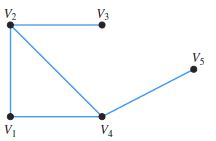
\includegraphics{week2/adj}
\end{figure}
\begin{enumerate}
\item
Determine the adjacency matrix $\bm A$ of the graph.
\item
Compute $\bm A^2$. What do the entries in the first row of $\bm A^2$ tell you about walks of length $2$ that start from $V_1$?
\item
Compute $\bm A^3$. How many walks of length $3$
are there from $V_2$ to $V_3$? How many walks of
length \textit{less than} or \textit{equal} to $3$ are there from $\bm V_2$ to $\bm V_4$?
\end{enumerate}
\end{enumerate}
%%
\chapter{Week4}

\section{Convergence}\index{week4_Friday_lecture}

\begin{definition}[Convergent]
An infinite sequence $\{z_n\}$ of complex numbers has a limit $z_0$, if for $\forall$ $\varepsilon>0$, there exists a positive integer $n_0$ such that
\[
\begin{array}{ll}
|z_n-z|<\varepsilon,
&
\mbox{whenever }n>n_0
\end{array}
\]
We say the sequence $z_n$ converges to $z$ and write as
\[
\lim_{n\to\infty}z_n=z
\]
When the sequence does not have a limit, then it diverges.
\end{definition}
The uniqueness of limit of a seuqnece is guaranteed.

\begin{proposition}
For $z_n=x_n+iy_n$, we have 
\[
\lim_{n\to\infty}z_n=x+iy
\]
if and only if
\[
\begin{array}{lll}
\lim_{n\to\infty}x_n=x,
&
\mbox{and}
&
\lim_{n\to\infty}y_n=y
\end{array}
\]
\end{proposition}

\begin{definition}[Convergent Series]
An infinite \emph{series} $\sum_{n=1}^\infty z_n$ of complex numbers converges to the sum $S$ if the partial sum sequences
\[
S_N=\sum_{n=1}^Nz_n
\]
converges to $S$, then we write
\[
\sum_{n=1}^\infty z_n=S.
\]
\end{definition}

\begin{proposition}
For $z_n=x_n+iy_n$, we have 
\[
\sum_{n=1}^\infty z_n=X+iY
\]
if and only if
\[
\begin{array}{lll}
\sum_{n=1}^\infty x_n=X
&
\mbox{and}
&
\sum_{n=1}^\infty y_n=Y
\end{array}
\]
\end{proposition}

\begin{proposition}
The series $\sum_{n=1}^\infty z_n$ converges implies that $\lim_{n\to\infty}z_n=0$.
\end{proposition}

\begin{definition}[Absolute Convergence]
The series $\sum_{n=1}^\infty z_n$ is said to be \emph{absolutely convergent} if
\[
\sum_{n=1}^\infty|z_n|
\]
converges, i.e., $\sum_{n=1}^\infty|x_n|$ and $\sum_{n=1}^\infty|y_n|$ converge.
\end{definition}
\begin{proposition}
Absolute convergence implies convergence
\end{proposition}

\begin{definition}[Remainder]
The \emph{remainder} $\rho_N$ of a series after $N$ terms is defined by:
\[
\rho_N=\sum_{n=N+1}^\infty S_n
\]
\end{definition}
\begin{proposition}
A series converges to a number $S$ iff the sequence of remainders tends to zero.
\end{proposition}

It's easy to verifty that
\[
\sum_{n=0}^\infty z_n=\frac{1}{1-z},\qquad\mbox{whenever }|z|<1
\]
with the aid of partial sums and remainders.

\subsection{Taylor Series}
\begin{definition}[Power Series]
The power series has the form
\[
\sum_{n=0}^\infty a_n(z-z_0)^n
\]
\end{definition}

\begin{theorem}[Convergent of Taylor Series]
Suppose $f$ is \emph{analytic} on $|z-z_0|<R$, then 
\begin{equation}
f(z)=\sum_{n=0}^\infty \frac{f^{(n)}(z_0)}{n!}(z-z_0)^n,
\end{equation}
for $|z-z_0|<R$, i.e., $f(z)$ admits its Taylor expansion at $z=z_0$ in this rigion.
\end{theorem}
\begin{remark}
Typically, when $z_0=0$, we say this series is the \emph{Maclaurin series}.
\end{remark}
\begin{proof}
\textbf{Step 1: Applying Cauchy Integral Formula.}
For fixed $z$, let $r:=|z-z_0|<R$ and take $r_0$ such that $r<r_0<R$. Construct a contour $C_0:\{z\in\mathbb{C}\mid |z-z_0|=r_0\}$ in the positive sense, which follows that
\begin{subequations}
\begin{align}
f(z)&=\frac{1}{2\pi i}\int_{C_0}\frac{f(s)}{s-z}\diff s\label{Eq:4:2:b}
\end{align}

\textbf{Step 2: Expand $1/(s-z)$.} With some calculation, we obtain
\begin{align}\label{Eq:4:2}
\frac{1}{s-z}&=\frac{1}{s-z_0}\cdot\frac{1}{1-\frac{z-z_0}{s-z_0}}\\
&=\frac{1}{s-z_0}\left\{1+\frac{z-z_0}{s-z_0}+\cdots+(\frac{z-z_0}{s-z_0})^{N-1}+\frac{(\frac{z-z_0}{s-z_0})^{N}}{1 - \frac{z-z_0}{s-z_0}}\right\}\label{Eq:4:2:d}\\
&=\frac{1}{s-z_0}+\frac{z-z_0}{(s-z_0)^2}+\cdots+\frac{(z-z_0)^{N-1}}{(s-z_0)^N}+\frac{(z-z_0)^N}{(s-z)(s-z_0)^N}\label{Eq:4:2:e}
\end{align}
where $(\ref{Eq:4:2:d})$ is because that
\[
\frac{1}{1-c}=1+c+c^2+\cdots+c^{N-1}+\frac{c^N}{1-c}. 
\]
Substituting (\ref{Eq:4:2:e}) into (\ref{Eq:4:2:b}), we obtain
\begin{align*}
f(z)&=\frac{1}{2\pi i}\int_{C_0}\left\{\frac{f(s)}{(s-z_0)}+\frac{f(s)(z-z_0)}{(s-z_0)^2}+\cdots+\frac{f(s)(z-z_0)^{N-1}}{(s-z_0)^N}+\frac{f(s)(z-z_0)^N}{(s-z)(s-z_0)^N}
\right\}\\
&=f(z_0)+f'(z_0)(z-z_0)+\cdots+\frac{f^{(N-1)}(z_0)}{(N-1)!}(z-z_0)^{N-1}+\rho_N(z)
\end{align*}
with
\begin{equation}\label{Eq:4:2:e}
\rho_N(z)=\frac{(z-z_0)^B}{2\pi i}\int_{C_0}\frac{f(s)}{(s-z)(s-z_0)^N}\diff s
\end{equation}

\textbf{Step 3: Show that $\rho_N(z)$ is convergent.}
\begin{align}
|\rho_N(z)|&\le\frac{|z-z_0|^N}{2\pi}\int_{C_0}\frac{|f(s)|}{|s-z||s-z_0|^N}|\diff s|\\
&\le\frac{r^N}{2\pi}\int_{C_0}\frac{M}{(r_0-r)r_0^N}|\diff s|\\
&=\frac{Mr_0}{r_0-r}\left(\frac{r}{r_0}\right)^N
\end{align}
where we suppose $|f(s)|\le M$ on $C_0$; and $|s-z|\ge|s-z_0| - |z-z_0| = r_0-r$. Therefore,
\[
\rho_N(z)\to0
\]
since $r<r_0$ and $(r/r_0)^N\to0$.
\end{subequations}




\end{proof}

\begin{example}
\begin{enumerate}
\item
For $f(z)=e^z$, which is analytic for $|z-0|<\infty$, thus we have
\[
e^z=\sum_{n=0}^\infty\frac{z^n}{n!},\qquad |z|<\infty
\]
\item
For $f(z)=\sin z=\frac{e^{iz} - e^{-i}}{2i}$, which is analytic for $|z-0|<\infty$, thus we have $f^{(2n)}(0)=0; f^{(2n+1)}(0)=(-1)^n$, and therefore
\[
\sin z=\sum_{n=0}^\infty\frac{(-1)^n}{(2n+1)!}z^{2n+1},\qquad |z|<\infty
\]
\item
For $f(z)=\frac{1}{1-z}$, which is analytic for $|z-0|<1$, we have $f^{(0)}=n!$, and therefore
\[
\frac{1}{1-z}=\sum_{n=0}^\infty\frac{n!}{n!}z^n=\sum_{n=0}^\infty z^n,\qquad |z|<1
\]
\item
For $f(z)=\frac{1}{z}\cdot\frac{1}{1+z}$, we have
\[
\frac{1}{1+z}=\sum_{n=0}^\infty(-z)^n,\qquad |z|<1,
\]
and therefore
\[
\frac{1}{z+z^2}=\frac{1}{z}+\sum_{n=1}^\infty(-1)^nz^{n-1},\qquad 0<|z|<1
\]
\end{enumerate}
\end{example}
\subsection{Laurent Series}
We cannot apply Taylor expansion at a non-analytic point. Fortunately, we can find another series representation for $f(z)$ that involving positive and negative powers of $(z-z_0)$
\begin{definition}[Laurent Series]
The \emph{Laurent series} has the form
\[
\sum_{n=0}^\infty a_n(z-z_0)^n+\sum_{n=1}^\infty\frac{b_n}{(z-z_0)^n}
\]
\end{definition}
\begin{theorem}
Suppose $f$ is analytic throughout an \emph{annular domain} $R_1<|z-z_0|<R_2$. Let $C$ be any \emph{positively oriented simple closed contour} around $z_0$ and lying in that domain. Then
\begin{subequations}
\begin{equation}
f(z)=\sum_{n=0}^\infty a_n(z-z_0)^n+\sum_{n=1}^\infty\frac{b_n}{(z-z_0)^n},\qquad
R_1<|z-z_0|<R_2
\end{equation}
with
\begin{align}
a_n&=\frac{1}{2\pi i}\int_C\frac{f(z)}{(z-z_0)^{n+1}}\diff z,\qquad n=0,1,2,\dots\\
b_n&=\frac{1}{2\pi i}\int_C\frac{f(z)}{(z-z_0)^{-n+1}}\diff z,\qquad n=1,2,\dots
\end{align}
\end{subequations}

\end{theorem}
\begin{remark}
The Laurent series is often written as the form
\[
f(z)=\sum_{n=-\infty}^\infty c_n(z-z_0)^n,\qquad R_1<|z-z_0|<R_2,
\]
where
\[
c_n=\frac{1}{2\pi i}\int_C\frac{f(z)}{(z-z_0)^{n+1}}\diff z,\qquad n=0,\pm1,\pm2,\dots
\]
When $f$ is analytic on $|z-z_0|<R_2$, we have $b_n=0,a_n=\frac{f^{(n)}(z_0)}{n!}$, i.e., the Laurent series reduces to the Taylor series.
\end{remark}
\begin{proof}
\begin{itemize}
\item
For fixed $z$ in the domain, let $r=|z-z_0|$, and construct two positively oriented contours $C_i:\{z\in\mathbb{C}\mid|z-z_0|=r_i\},i=1,2$ such that $R_1<r_1<r<r_2<R_2$. (The reaon why we don't use the boundary is that the function is not analytic on the boundary but only interior to)
\item
Construct a circle $\gamma:\{s\in\mathbb{C}\mid s = z + \delta e^{i\theta},0\le\theta\le2\pi\}$, where the $\delta$ is picked such that $\gamma$ is contained in the interior between $C_1,C_2$. By Cauchy Integral Formula,
\begin{equation}
\int_{C_2}\frac{f(s)\diff s}{s-z}=\int_{C_1}\frac{f(s)\diff s}{s-z}+\int_{\gamma}\frac{f(s)\diff s}{s-z}
\end{equation}
Or equivalently,
\[
f(z)=\frac{1}{2\pi i}\int_{C_2}\frac{f(s)\diff s}{s-z}+\frac{1}{2\pi i}\int_{C_1}\frac{f(s)\diff s}{z-s}
\]
\item
By applying the same trick as (\ref{Eq:4:2}), we have
\begin{subequations}
\begin{equation}
f(z)=\sum_{n=0}^{N-1}a_n(z-z_0)^n+\rho_N(z)+\sum_{n=1}^N\frac{b_n}{(z-z_0)^n}+\sigma_N(z)
\end{equation}
with
\begin{align}
a_n&=\frac{1}{2\pi i}\int_{C_2}\frac{f(s)\diff s}{(s-z_0)^{n+1}}\\
b_n&=\frac{1}{2\pi i}\int_{C_1}\frac{f(s)\diff s}{(s-z_0)^{-n+1}}\\
\rho_N(z)&=\frac{(z-z_0)^N}{2\pi i}\int_{C_2}\frac{f(s)\diff s}{(s-z)(s-z_0)^N}\\
\sigma_N(z)&=\frac{(z-z_0)^{-N}}{2\pi i}\int_{C_1}\frac{f(s)\diff s}{(z-s)(s-z_0)^{-N}}
\end{align}
\end{subequations}
\item
Then we bound the term $\rho_N(z)$ and $\sigma_N(z)$. Suppose $|f(s)|\le M$ on $C_1,C_2$, and note that $|s-z|\ge r_2-r$ for $s\in C_2$; $|z-s|\ge r-r_1$ for $s\in C_1$:
\begin{align*}
\rho_N(z)&\le\frac{Mr_2}{r_2-r}\left(\frac{r}{r_2}\right)^N\\
\sigma_N(z)&\le\frac{Mr_1}{r-r_1}\left(\frac{r_1}{r}\right)^N
\end{align*}
\item
Finally, note that
\begin{align*}
a_n&=\frac{1}{2\pi i}\int_{C}\frac{f(s)\diff s}{(s-z_0)^{n+1}}\\
b_n&=\frac{1}{2\pi i}\int_{C}\frac{f(s)\diff s}{(s-z_0)^{-n+1}}\\
\end{align*}





\end{itemize}
\end{proof}

\begin{example}
\begin{enumerate}
\item
\[
f(z)=\frac{1}{z-1} - \frac{1}{z-2}
\]
This function has two singular points $1,2$. We take $z_0=0$.
\begin{itemize}
\item
When $z\in D_1=\{z:|z|<1\}$, we obtain the Taylor expansion:
\[
f(z)=-\sum_{n=0}^\infty z^n+\sum_{n=0}^\infty\frac{z^n}{2^{n+1}}=\sum_{n=0}^\infty(2^{-n-1}-1)z^n
\]
\item
When $z\in D_2=\{z:1<|z|<2\}$, we obtain the Laurent series:
\[
f(z)=\sum_{n=0}^\infty\frac{z^n}{2^{n+1}}+\sum_{n=1}^\infty\frac{1}{z^n}
\]
\item
When $z\in D_3=\{z:|z|>2\}$, we obtain
\[
f(z)=\sum_{n=1}^\infty\frac{1-2^{n-1}}{z^n}
\]
\end{itemize}
\item
Expand $f(z)=\frac{-z}{(z-1)(z-3)}$ near $z_0=1$, and find the domain of expansion.

The expansion should be the laurent series with domain of expansion $0<|z-1|<2$.
\[
f(z)=\frac{1/2}{z-1}-\frac{3/2}{z-3}=\frac{1/2}{z-1}+\sum_{n=0}^\infty\frac{3}{2^{n+2}}(z-1)^n
\]





\end{enumerate}
\end{example}
\subsection{Power Series}
For power series
\begin{equation}\label{Eq:4:6}
\sum_{n=0}^\infty a_n(z-z_0)^n
\end{equation}
, first we study the range of its convergence.
\begin{theorem}\label{The:4:3}
If the power series (\ref{Eq:4:6}) converges at $z=z_1(\ne z_0)$, then it is \emph{absolutely convergent} at each point in the disk $|z-z_0|<|z_1-z_0|$.
\end{theorem}
\begin{proof}
For any point $z$ around the disk, we have, we have
\[
\left|\frac{z-z_0}{z_1-z_0}\right|:=q<1,
\]
which follows that
\[
|a_n(z-z_0)^n|=|a_n(z_1-z_0)^n|\left|\frac{z-z_0}{z_1-z_0}\right|^n\le Mq^n,
\]
where $|a_n(z_1-z_0)^n|\le M$ since $z_1$ makes the series convergent. By Comparison test, we conclude (\ref{Eq:4:6}) is absolutely convergent.
\end{proof}
\begin{definition}[Uniform convergence]
The series (\ref{Eq:4:6}) is said to be \emph{uniformly convergent} for $|z-z_0|<R$ if as $N\to\infty$,
\[
\sup_{|z-z_0|<R}|\rho_N(z)|\to0
\]
\end{definition}

\begin{theorem}
If the power series (\ref{Eq:4:6}) converges at $z=z_1(\ne z_0)$, then it must be uniformly convergent for any closed circle $|z-z_0|\le \rho$ ($\rho<|z_1-z_0|$).
\end{theorem}
\begin{proof}
Notice that for any $\rho<|z_1-z_0|$, for any $z$ in that closed circle, we have
\[
|a_n(z-z_0)^n|\le |a_n\rho^n|
\]
Due to the conclusion in Theorem(\ref{The:4:3}), we conclude $\sum_{n=1}^\infty |a_n|\rho^n$ is convergent, and therefore $(\ref{Eq:4:6})$ is uniformly convergent.

\end{proof}
Now we are curious about whether the power series is analytic. First we show under which condition does the power series is continuous.
\begin{theorem}
The series (\ref{Eq:4:6}) represents a continuous function at each point inside the circle of convergence.
\end{theorem}

\begin{theorem}
The sum $S(z)$ of power series is analytic at each point $z$ interior to the circle convergence of that series.
\end{theorem}






















%%\include{week3/Lecture_2}
%
\chapter{Week2}
\section{Monday}\index{week2_Tuesday_lecture}
\subsection{Reviewing and Announments}
Tutorial: Thursday 7:00pm -9:00pm, ChengDao 208

Homework is due every Monday.

The first homework has been uploaded.

To proof the optimality condition in $\mathbb{R}^n$, we set $h(t) = f(x^*+td)$ for fixed $x^*$ and $d$. It follows that
\[
h'(t)=\nabla\trans f(x^*+td)d
\]
and
\[
h''(t)=d\trans\nabla^2f(x^*+td)d
\]
By the optimality condition for $\mathbb{R}$, we derive the necessary condition:
\[
\left\{
\begin{aligned}
\mbox{$h'(0)=\nabla\trans f(x^*)d=0$ for $\forall d$}\implies \mbox{$\nabla f(x^*)=0$;}\\
\mbox{$h''(0)=d\trans\nabla^2f(x^*)d=0$ for $\forall d$}
\implies
\mbox{$\nabla^2f(x^*)\succeq0$}
\end{aligned}
\right.
\]
together with the sufficient condition:
\[
\left\{
\begin{aligned}
\mbox{$\nabla f(x^*)=0$;}\\
\mbox{$\nabla^2f(x^*)\succ0$}
\end{aligned}
\right.
\]
\subsection{Quadratic Function Case Study}
Given a quadratic function 
\[
f(\bm x) =\frac{1}{2}\bm x\trans\bm Q\bm x+\bm b\trans\bm x
\]
w.l.o.g., assume the matrix $\bm Q$ is symmetric (recall the quadratic section studied in linear algebra).


\begin{definition}[Stationarity]
A point $\bm x^*$ is said to be the stationary point of $f(\bm x)$ if $\nabla f(\bm x^*)=\bm0$.
\end{definition}
To minimize such a function without constraint, we apply the optimality condition:
\begin{enumerate}
\item
The first order optimality condition is given by:
\[
\nabla f(\bm x) = \bm Q\bm x+\bm b=\bm0
\]
The stationary point of the quadratic function $f(\bm x)$ exists iff $\bm b\in\mathcal{C}(\bm Q).$
\item
The second order necessary condition should be:
\[
\nabla^2 f(\bm x)=\bm Q\succeq0
\]
\end{enumerate}
For this special case, if $\bm Q\succeq0$, then $f(\bm x)$ is convex, the solutions to $\nabla f(\bm x) =\bm0$ are local minimum points. Furthermore, they are global minimum points (prove by Taylor Expansion). However, for general functions, we cannot obtain such good results.

\paragraph{Least Squares Problem} Such a problem has been well-studied in statistics given by:
\[
\min_{\bm x}f(\bm x):=\frac{1}{2}\|\bm{Ax}-\bm b\|_2^2
\]
The first order derivative of the minimizer should satisfy:
\[
\nabla f(\bm x)=\bm A\trans(\bm A\bm x-\bm b)
\]
Note that $\bm A\trans\bm b\in\mathcal{C}(\bm A\trans\bm A)$, thus the least squares problem always has a solution. However, such a solution is not unique unless $\bm A$ is full rank.
\paragraph{A Non-trival Quadratic Function}
To minimize the function
\[
f(x,y)=\frac{1}{2}(\alpha x^2+\beta y^2)-x
\] 
We take the first order derivative to be zero:
\[
\nabla f(x,y)=\begin{bmatrix}
\alpha x-1\\\beta y
\end{bmatrix}=\bm0
\]
The second order derivative is given by:
\[
\nabla^2 f(x,y)=\begin{bmatrix}
\alpha&0\\0&\beta
\end{bmatrix}
\]
The optimal solutions depend on the value of $\alpha$ and $\beta$: (although we haven't introduce the definition for convex formally)
\begin{itemize}
\item
If $\alpha,\beta>0$, then this problem is \emph{strongly convex}. By the necessary and sufficient optimality condition for convex problem, we find that $(\frac{1}{\alpha},0)$ is the unique local minimum (It is also the global minimum by plotting the figure).
\item
If $\alpha=0$, this problem has no solution. The objective value $f(x,y)\to-\infty$ as $x\to
\infty$.
\item
If $\beta=0,\alpha>0$, this problem is convex.  By the necessary and sufficient optimality condition for convex problem, $\{(\frac{1}{\alpha},\xi)\mid \xi\in\mathbb{R}\}$ is the set of local minimum. (By plotting the graph, we find that such set is the set of global minimum points)
\item
For $\alpha>0,\beta<0$ case, this problem is non-convex. Actually, $f(x,y)\to-\infty$ as $y\to
\infty$. Hence, this problem has no global minimum point.
\end{itemize}

\paragraph{A Non-trival Function Study}
To minimize the function
\[
\begin{array}{ll}
\min&f(\bm y)=e^{y_1}+\cdots+e^{y_n}\\
\mbox{such that}&y_1+\cdots+y_n=S
\end{array}
\]
We can transform such a constrainted optimization problem into unconstrainted. Let $y_n=S-y_1-\cdots-y_{n-1}$ and substitute it into the objective function, it suffices to solve
\[
\min e^{y_1}+\cdots+e^{y_{n-1}}+e^{S-y_1-\cdots-y_{n-1}}
\]
The stationary point should satisfy:
\[
e^{y_i}=e^{S-y_1-\cdots-y_{n-1}},
\qquad
i=1,2,\dots,n-1
\]
Or equivalently, $y_1=y_2=\cdots=y_{n-1}=y_n$. Hence we derive the unique stationary point:
\[
y_1^*=y_2^*=\cdots=y_n^*=\frac{S}{n}
\]
The value on the stationary point is $f(y^*)=ne^{S/n}$. By checking the second order sufficient optimality condition,
\[
\frac{f}{\partial y_i\partial y_j}=\left\{
\begin{aligned}
e^{y_i}+e^{S-y_1-\cdots-y_{n-1}}&\quad i=j\\
e^{s-y_1-\cdots-y_{n-1}}&\quad i\ne j
\end{aligned}
\right.\implies
\nabla^2 f=e^{s-y_1-\cdots-y_{i-1}-y_i-y_{n-1}}\bm E
+\diag(e^{y_1},\dots,e^{y_{n-1}})
\]
where $\bm E$ is a matrix with entries all ones. Thus $\nabla^2 f\succ0$ for any stationary point. By the second order sufficient optimality condition, this stationary point is local minimum. Actually, for this special problem, this unique local minimum point is the global minimum.
\begin{remark}
In this problem, we find that this stationary point is the unique local minimum point, but the unique local minimum point is not necessarily the global minimum point, unless the function is \emph{coercive} or the feasible region is compact. Here is the counter-example: $f(x)=x^2-x^4$. We will discuss the definition for coercive in the future.
\end{remark}










%
\section{Thursday}\index{week5_Thursday_lecture}
\subsection{Orthogonality}
Recall that two vectors are orthogonal if their inner product is zero:
\[
\bm u\perp\bm v
\Longleftrightarrow
\inp{\bm u}{\bm v}=0
\]

Orthogonality among vectors has an important property:
\begin{proposition}
If \emph{nonzero} vectors $v_1,\dots,v_k$ are mutually orthogonal, i.e., $v_i\perp v_j$ for any $i\ne j$, then $\{v_1,\dots,v_k\}$ must be ind.
\end{proposition}
\begin{proof}
It suffices to show that 
\[
\alpha_1v_1+\dots+\alpha_kv_k=\bm 0 \implies
\alpha_i=0\text{ for any $i\in\{1,2,\dots,k\}$.}
\]
\begin{itemize}
\item
We do inner product to show $\alpha_1$ must be zero:
\[
\begin{aligned}
\inp{v_1}{\alpha_1v_1+\dots+\alpha_kv_k}
&=\inp{v_1}{\bm 0}=0\\
&=\alpha_1\inp{v_1}{v_1}+\alpha_2\inp{v_1}{v_2}+\dots+\alpha_k\inp{v_1}{v_k}\\
&=\alpha_1\inp{v_1}{v_1}=\alpha_1\|v_1\|_2^2\\
&=0
\end{aligned}
\]
Since $v_1\ne \bm 0$, we have $\alpha_1=0$.
\item
Similarly, we have $\alpha_i=0$ for $i=1,\dots,k$.
\end{itemize}
\end{proof}
Now we can also talk about orthogonality among spaces:
\begin{definition}[Subspace Orthogonality]
Two subspaces $\bm U$ and $\bm V$ of a vector space are \emph{orthogonal} if every vector $\bm u$ in $\bm U$ is \textit{perpendicular} to every vector $\bm v$ in $\bm V$:
\[
\begin{array}{lll}
\mbox{\emph{Orthogonal subspaces}}
&
\bm u\perp\bm v,
&
\forall\bm u\in\bm U,\bm v\in\bm V.
\end{array}
\]
\end{definition}
\begin{example}
Two walls look \textit{perpendicular} but they are not orthogonal subspaces! The meeting line is in both $\bm U$ and $\bm V$-and this line is not perpendicular to itself. Hence, two planes (both with dimension $2$ in $\mathbb{R}^{3}$) cannot be orthogonal subspaces.

\begin{figure}[H]
\centering
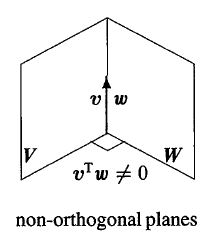
\includegraphics{week5/orthogonality}
\caption{Orthogonality is impossible when $\dim\bm U+\dim\bm V>\dim(\bm U\cup\bm V)$}
\end{figure}
\end{example}
\begin{remark}
When a vector is in two orthogonal subspaces, it \textit{must} be zero. It is \emph{perpendicular} to
itself. 
\\The reason is clear: this vector $\bm u\in\bm U$ and $\bm u\in\bm V$, so $\inp{\bm u}{\bm u}=0$. It has to be zero vector.
\end{remark}
If two subspaces are perpendicular, their basis must be ind.
\begin{theorem}
Assume $\{u_1,\dots,u_k\}$ is the basis for $\bm U$, $\{v_1,\dots,v_l\}$ is the basis for $\bm V.$ If $\bm U\perp\bm V$ ($u_i\perp v_j$ for $\forall i,j$), then $u_1,u_2,\dots,u_k,v_1,v_2,\dots,v_l$ must be ind.
\end{theorem}
\begin{proof}
Suppose there exists $\{\alpha_1,\dots,\alpha_k\}$ and $\{\beta_1,\dots,\beta_l\}$ such that
\[
\alpha_1u_1+\dots+\alpha_ku_k+\beta_1v_1+\dots+\beta_lv_l=\bm 0
\]
then equivalently,
\[
\alpha_1u_1+\dots+\alpha_ku_k=-(\beta_1v_1+\dots+\beta_lv_l).
\]
Then we set $\bm w=\alpha_1u_1+\dots+\alpha_ku_k$, obviously, $\bm w\in\bm U$ and $\bm w\in\bm V$.

 Hence it must be zero (This is due to remark above). Thus we have
\begin{gather*}
\alpha_1u_1+\dots+\alpha_ku_k=\bm 0\\
\beta_1v_1+\dots+\beta_lv_l=\bm 0.
\end{gather*}
Due to the independence, we have $\alpha_i=0$ and $\beta_j=0$ for $\forall i,j$. 
\end{proof}
\begin{corollary}
For subspaces $\bm U$ and $\bm V$, we obtain
\[
\dim(\bm U\cup\bm V)\le \dim(\bm U) + \dim(\bm V).
\]
\end{corollary}
For subspaces $\bm U$ and $\bm V\in\mathbb{R}^{n}$, if $\mathbb{R}^{n}=\bm U\cup\bm V$, and moreover, $n=\dim(\bm U)+\dim(\bm V)$, then we say $\bm V$ is the \emph{orthogonal complement} of $\bm U$.
\begin{definition}[orthogonal complement]
For subspaces $\bm U$ and $\bm V\in\mathbb{R}^{n}$, if $\dim(\bm U)+\dim(\bm V)=n$ and $\bm U\perp\bm V$, then we say $\bm V$ is the \emph{orthogonal complement} of $\bm U$. We denote $\bm V$ as $\bm U^{\perp}$.

Moreover, $\bm V=\bm U^{\perp}$ iff $\bm V^{\perp}=\bm U$.
\end{definition}
\begin{example}
Suppose $\bm U\cup\bm V=\mathbb{R}^{3}$, $\bm U=\Span\{\bm e_1,\bm e_2\}$. If $\bm V$ is the orthogonal complement of $\bm U$, then $\bm V=\Span\{\bm e_3\}$.
\end{example}

Next we study the relationship between the null space and the row space in $\mathbb{R}^n$.
\begin{theorem}[Fundamental theorem for linear alegbra, part 2] Given $\bm A\in\mathbb{R}^{m\times n}$,

\emph{$N(\bm A)$ is the orthogonal complement of the row space of $\bm A$, $\mathcal{C}(\bm A\trans)$ (in $\mathbb{R}^{n}$).}

\emph{$N(\bm A\trans)$ is the orthogonal complement of the column space $\mathcal{C}(\bm A)$ (in $\mathbb{R}^{m}$).}
\end{theorem}
\begin{proof}
\begin{itemize}
\item
Firstly, we show $\dim(N(\bm A))+\dim(\mathcal{C}(\bm A\trans))=n$:

We know that $\dim(N(\bm A))=n-r$ and $\dim(\mathcal{C}(\bm A\trans)) = r$, where $r=\rank(\bm A)$.

Hence $\dim(N(\bm A))+\dim(\mathcal{C}(\bm A\trans))=n$.
\item
Then we show $N(\bm A)\perp \mathcal{C}(\bm A\trans)$:

For any $x\in N(\bm A)$, if we set $\bm A=\begin{bmatrix}
a_1\trans\\a_2\trans\\\vdots\\a_m\trans
\end{bmatrix}$, then we obtain:
\[
\bm{Ax}=\begin{bmatrix}
a_1\trans\\a_2\trans\\\vdots\\a_m\trans
\end{bmatrix}\begin{bmatrix}
\bm x
\end{bmatrix}=\begin{bmatrix}
0\\0\\\vdots\\0
\end{bmatrix}
\]
Hence \textit{every row has a zero product with} $\bm x$, i.e., $\inp{a_i}{\bm x}=0$ for $\forall i\in\{1,2,\dots,m\}$.

For any $y=\sum_{i=1}^m\alpha_ia_i\in \mathcal{C}	(\bm A\trans)$, we obtain:
\[
\begin{aligned}
\inp{\bm x}{y}&=\inp{y}{\bm x}=\inp{\sum_{i=1}^m\alpha_ia_i}{\bm x}\\
&=\sum_{i=1}^{m}\alpha_i\inp{a_i}{\bm x}=0.
\end{aligned}
\]
Hence $\bm x\perp y$ for $\forall \bm x\in N(\bm A)$ and $y\in \mathcal{C}(\bm A\trans)$.\\
\end{itemize}
Hence $N(\bm A)^{\perp}=\mathcal{C}(\bm A\trans)$. Similarly, we have $N(\bm A\trans)^{\perp}=\mathcal{C}(\bm A)$. 
\end{proof}

\begin{corollary}
$\bm{Ax}=\bm b$ is solvable if and only if $\bm y\trans\bm A=\bm 0$ implies $\bm y\trans\bm b$=0.
\end{corollary}
\begin{proof} The following statements are equivalent:
\begin{itemize}
\item
$\bm{Ax}=\bm b$ is solvable.
\item
$\bm b\in \mathcal{C}(\bm A)$.
\item
$\bm b\in N(\bm A\trans)^{\perp}$
\item
$\bm y\trans\bm b=0$ for $\forall y\in N(\bm A\trans)$
\item
Given $\bm y\trans\bm A=\bm 0$, i.e., $y\in N(\bm A\trans)$, it implies $\bm y\trans\bm b=0$.
\end{itemize}
\end{proof}
The \emph{Inverse Negative Proposition} is more commonly useful:
\begin{corollary}
$\bm{Ax}=\bm b$ has no solution if and  and only if $\exists \bm y$ s.t. $\bm y\trans\bm A=0$ and $\bm y\trans\bm b\ne 0$.
\end{corollary}
We could extend this corollary into general case:
\begin{remark}
\begin{theorem}\label{theorem_12.3}
$\bm{Ax}\ge\bm b$ has no solution if and only if $\exists \bm y\ge\bm 0$ such that $\bm y\trans\bm A=\bm 0$ and $\bm y\trans\bm b\ge \bm 0$.
\end{theorem}
$\bm y\trans\bm A=0$ requires that there exists one linear combination of the row space to be zero.

The complete proof for this theorem is not required in this course. We only show the necessity case.
\begin{proof}[Necessity case.]
Suppose $\exists \bm y\ge\bm 0$ such that $\bm y\trans\bm A=\bm 0$ and $\bm y\trans\bm b\ge \bm 0$. Assume there exists $x^{*}$ such that $\bm Ax^{*}\ge\bm b$. By postmultiplying $\bm y\trans$ we have 
\[\bm y\trans\bm Ax^{*}\ge\bm y\trans\bm b>\bm 0
\implies 
\bm 0>\bm 0.
\]
which is a contradiction!
\end{proof}
\end{remark}

\begin{example}
Given the system 
\begin{align}
x_1+x_2&\ge1\label{Eq:6:3}
\\
-x_1&\ge-1\label{Eq:6:4}
\\
-x_2&\ge2\label{Eq:6:5}
\end{align}
Eq.(\ref{Eq:6:3})$\x$1+Eq(\ref{Eq:6:4})$\x$1+Eq.(\ref{Eq:6:5})$\x$1 gives
\[
0\ge 2
\]
which is a contradiction!\\
So the key idea of theorem (\ref{theorem_12.3}) is to construct a linear combination of row space to let it become zero. If the right hand is larger than zero, then this system has no solution.
\end{example}
\begin{remark}
\begin{corollary}
If $\bm A=\bm A\trans$, then $N(\bm A\trans)^{\perp}=\mathcal{C}(A)=\mathcal{C}(\bm A\trans)=N(\bm A)$.
\end{corollary}
\begin{corollary}\label{corollary_12.5}
The system $\bm{Ax}=\bm b$ may not have a solution, but $\bm A\trans\bm A\bm x=\bm A\trans\bm b$ always have at least one solution for $\forall\bm b$.
\end{corollary}
\begin{proof}
Since $\bm A\trans\bm A$ is symmetric, we have $\mathcal{C}(\bm A\trans\bm A)=\mathcal{C}(\bm A\bm A\trans)$. Show by yourself that $\mathcal{C}(\bm A\bm A\trans)=\mathcal{C}(\bm A\trans)$, hence $\mathcal{C}(\bm A\trans\bm A)=\mathcal{C}(\bm A\trans)$.

For any vector $\bm b$, we have $\bm A\trans\bm b\in \mathcal{C}(\bm A\trans)\implies\bm A\trans\bm b\in \mathcal{C}(\bm A\trans\bm A)$, which means there exists a linear combination of the columns of $\bm A\trans\bm A$ that equals to $\bm b$.

Or equivalently, there exists a solution to $\bm A\trans\bm A\bm x=\bm A\trans\bm b$.
\end{proof}
\begin{corollary}\label{corollary_12.6}
$\bm A\trans\bm A$ is invertible if and only if $\bm A$ is full column rank, i.e., columns of $\bm A$ are ind.
\end{corollary}
\begin{proof}
We have shown that $C(\bm A\trans\bm A)=C(\bm A\trans)$.

Hence $C(\bm A\trans\bm A)^{\perp}=C(\bm A\trans)^{\perp}\implies N(\bm A\trans\bm A)=N(\bm A)$.

Thus, the following statements are equivalent:
\begin{itemize}
\item
$\bm A$ has ind. columns
\item
$N(\bm A)=\{\bm 0\}$
\item
$N(\bm A\trans\bm A)=\{\bm 0\}$
\item
$\bm A\trans\bm A$ is invertible.
\end{itemize}
\end{proof}
\end{remark}
\subsection{Least Squares Approximations}
The linear system $\bm{Ax}=\bm b$ often has no solution, if so, what should we do?

We cannot always get the error $\bm e=\bm b-\bm{Ax}$ down to zero, so we want to use \textit{least square method} to minimize the error. In other words, our goal is to
\[
\min_{\bm x\in\mathbb{R}^n}\bm e^2:=\min_{\bm x}\|\bm{Ax}-\bm b\|^2=\sum_{i=1}^{m}(a_i\trans\bm x-b_i)^2
\]
where $\bm A\in\mathbb{R}^{m\times n}$ and $\bm b\in\mathbb{R}^m$. The minimizer $\bm x$ is called the \emph{linear least squares solution}.

\subsubsection{Least Squares by Convex Optimization}
Firstly, you should know some basic calculus knowledge for matrix:
\paragraph{The Chian Rule} Given two vectors $f(x),g(x)$ of appropriate size,
\[
\frac{\partial(f\trans g)}{\partial x}=\frac{\partial f(x)}{\partial x}g(x)+\frac{\partial g(x)}{\partial x}f(x)
\]
\paragraph{Examples of Matrix Derivative}
\begin{align}
\frac{\partial(a\trans \bm x)}{\partial \bm x}&=a\\
\frac{\partial(a\trans \bm A\bm x)}{\partial \bm x}&=\frac{\partial((\bm A\trans a)\trans\bm x)}{\partial \bm x}=\bm A\trans a\\
\frac{\partial(\bm A\bm x)}{\partial \bm x}&=\bm A\trans\\
\frac{\partial(\bm x\trans\bm A\bm x)}{\partial \bm x}&=\bm A\bm x+\bm A\trans\bm x
\end{align}

Thus, in order to minimize $\|\bm{Ax}-\bm b\|^2=(\bm{Ax}-\bm b)\trans(\bm{Ax}-\bm b)$, it suffices to let its \emph{derivative} with respect to $\bm x$ to be \emph{zero.} (Since $\|\bm{Ax}-\bm b\|^2$ is convex, which will be discussed in detail in other courses.) Hence we have:
\[\begin{aligned}
\frac{\partial (\bm{Ax}-\bm b)\trans(\bm{Ax}-\bm b)}{\partial \bm x}&=\frac{\partial(\bm{Ax}-\bm b)}{\partial \bm x}(\bm{Ax}-\bm b)+\frac{\partial(\bm{Ax}-\bm b)}{\partial \bm x}(\bm{Ax}-\bm b)\\
&=2\frac{\partial(\bm{Ax}-\bm b)}{\partial \bm x}(\bm{Ax}-\bm b)\\
&=2(\frac{\partial(\bm A\bm x)}{\partial \bm x}-\frac{\partial(\bm b)}{\partial \bm x})(\bm{Ax}-\bm b)\\
&=2\bm A\trans(\bm{Ax}-\bm b)=\bm 0.
\end{aligned}
\]
Or equivalently, 
\[
\bm A\trans\bm{Ax}=\bm A\trans\bm b.
\]
According to corollary (\ref{corollary_12.5}), this equation always exists a solution. This equation is called the \emph{normal equation}.
\begin{theorem}\label{theorem_12.4}
A vector $\bm x_{\text{LS}}$ is an optimal solution to the least squares problem
\begin{subequations}
\begin{equation}
\min_{\bm x\in\mathbb{R}^n}\|\bm b-\bm{Ax}\|_2^2
\end{equation}
if and only if it satisfies
\begin{equation}
\bm A\trans\bm A\bm x_{\text{LS}} = \bm A\trans\bm b.
\end{equation}
\end{subequations}
\end{theorem}
\subsubsection{Fit a stright line}
Given a collection of data $(\bm x_i,y_i)$ for $i=1,\dots,m$, we can use a stright line to fit these points:
\[
\left\{
\begin{aligned}
y_1&=a_0+a_1x_{1,1}+a_2x_{1,2}+\dots+a_nx_{1,n}+\varepsilon_1\\
y_2&=a_0+a_1x_{2,1}+a_2x_{2,2}+\dots+a_nx_{2,n}+\varepsilon_2\\
\vdots\\
y_m&=a_0+a_1x_{m,1}+a_2x_{m,2}+\dots+a_nx_{m,n}+\varepsilon_m
\end{aligned}
\right.
\]
Our fit line is 
\[
\hat y=a_0+a_1x_1+a_2x_2+\dots+a_nx_n
\]
In \textit{compact matrix form}, we have
\[
\begin{bmatrix}
y_1\\y_2\\\vdots\\y_n
\end{bmatrix}
=\begin{bmatrix}
1&x_{1,1}&x_{1,2}&\dots&x_{1,n}\\
1&x_{2,1}&x_{2,2}&\dots&x_{2,n}\\
\vdots&\vdots&&&\\
1&x_{m,1}&x_{m,2}&\dots&x_{m,n}\\
\end{bmatrix}\begin{bmatrix}
a_0\\a_1\\a_2\\\vdots\\a_{n}
\end{bmatrix}+\begin{bmatrix}
\varepsilon_1\\\varepsilon_2\\\vdots\\\varepsilon_m
\end{bmatrix}
\]
Or equivalently, we have 
\[
\bm y=\bm{Ax}+\bm \varepsilon
\]
where $\bm A =\begin{bmatrix}
1&x_{1,1}&x_{1,2}&\dots&x_{1,n}\\
1&x_{2,1}&x_{2,2}&\dots&x_{2,n}\\
\vdots&\vdots&&&\\
1&x_{m,1}&x_{m,2}&\dots&x_{m,n}\\
\end{bmatrix}_{m\times (n+1)}$, $\bm x=\begin{bmatrix}
a_0\\a_1\\a_2\\\vdots\\a_{n}
\end{bmatrix}_{(n+1)\times 1}$, $\bm \varepsilon=\begin{bmatrix}
\varepsilon_1\\\varepsilon_2\\\vdots\\\varepsilon_m
\end{bmatrix}_{m\times 1}$.\\
Our goal is to minimize $\|\hat{\bm y}-\bm y\|^2=\|\bm{Ax}-\bm y\|^2$. Then by theorem (\ref{theorem_12.4}), it suffices to sovle $\bm A\trans\bm A\bm x=\bm A\trans\bm y$.

\subsection{Projections}
In corollary (\ref{corollary_12.6}), we know that if $\bm A$ has ind. columns, then $\bm A\trans\bm A$ is invertible. On this condition, the normal equation $\bm A\trans\bm A\bm x=\bm A\trans\bm b$ has the unique solution $\bm x^{*}=(\bm A\trans\bm A)^{-1}\bm A\trans\bm b$, which follows that the error $\bm b-\bm A\bm x^{*}$ is minimized. Note that $\bm A\bm x^{*}=\bm A(\bm A\trans\bm A)^{-1}\bm A\trans\bm b$ is \emph{approximately} equal to $\bm b$. 
\begin{itemize}
\item
If $\bm b$ and $\bm{A}\bm x^{*}$ are exactly in the same space, i.e., $\bm b\in\mathcal{C}(\bm A)$, then $\bm{A}\bm x^{*}=\bm b$. The error is equal to zero.
\item
Otherwise, just as the Figure (\ref{figure_12.2}) shown, $\bm A\bm x^{*}$ is the projection of $\bm b$ to subspace $\mathcal{C}(\bm A)$.
\end{itemize}
\begin{figure}[t]
\centering
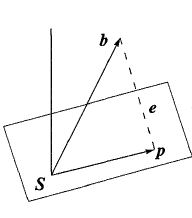
\includegraphics{week5/projection}
\caption{The projection of $\bm b$ onto a subspace $\bm S:=\mathcal{C}(\bm A)$.}\label{figure_12.2}
\end{figure}
\begin{definition}[Projection]
Let $\bm S\in\mathbb{R}^{m}$ be a non-empty closed set and $\bm b\in\mathbb{R}^m$ be given. Then the projection of $\bm b$ onto the set $\bm S$ is the solution to
\[
\min_{\bm z\in\bm S}\|\bm z-\bm b\|_2^2,
\]
where we use notation $\Proj_{\bm S}(\bm b)$ to denote the projection of $\bm b$ onto $\bm S$.
\end{definition}
By definition, the projection of $\bm b$ onto the subspace $\mathcal{C}(\bm A)$ is given by 
\[
\Proj_{\mathcal{C}(\bm A)}(\bm b):=\bm A\bm x^*,\quad
\text{where }\bm x^*=\arg\min_{\bm x\in\mathbb{R}^n}\|\bm{Ax} - \bm b\|.
\]

\begin{definition}[Projection matrix]
Given the projection
\[
\Proj_{C(\bm A)}(\bm b):=\bm A\bm x^{*}=\bm A(\bm A\trans\bm A)^{-1}\bm A\trans\bm b,
\]
since $[\bm A(\bm A\trans\bm A)^{-1}\bm A\trans]\bm b$,
we call the projection operator $\bm P:=\bm A(\bm A\trans\bm A)^{-1}\bm A\trans$ as the \emph{projection matrix} of $\bm A$.
\end{definition}
\begin{definition}[Idempotent]
Let $\bm A$ be a \emph{square} matrix that satisfies $\bm A=\bm A\bm A$, then $\bm A$ is called an \emph{idempotent} matrix.
\end{definition}
Let's show that the projection matrix is \textit{idempotent}:
\[
\begin{aligned}
\bm P^{2}&=\bm A(\bm A\trans\bm A)^{-1}\bm A\trans\bm A(\bm A\trans\bm A)^{-1}\bm A\trans\\
&=\bm A(\bm A\trans\bm A)^{-1}(\bm A\trans\bm A)(\bm A\trans\bm A)^{-1}\bm A\trans\\
&=\bm A(\bm A\trans\bm A)^{-1}\bm A\trans=\bm P.
\end{aligned}
\]

\subsubsection{Observations}
\begin{itemize}
\item
Suppose $\bm b\in \mathcal{C}(\bm A)$, i.e., $\exists \bm x$ s.t. $\bm{Ax}=\bm b$. Then the projection of $\bm b$ is exactly $\bm b$:
\[
\begin{aligned}
\bm{Pb}&=\bm A(\bm A\trans\bm A)^{-1}\bm A\trans(\bm b)\\
&=\bm A(\bm A\trans\bm A)^{-1}\bm A\trans(\bm{Ax})\\
&=\bm A(\bm A\trans\bm A)^{-1}(\bm A\trans\bm A)\bm x\\
&=\bm{Ax}=\bm b.
\end{aligned}
\]
\item
Assume $\bm A$ has only one column, say, $\bm a$. Then we have
\[\begin{aligned}
\bm x^{*}&=(\bm A\trans\bm A)^{-1}\bm A\trans\bm b=\frac{\bm a\trans\bm b}{\bm a\trans\bm a}\\
\bm A\bm x^{*}&=\bm{Pb}=\bm A(\bm A\trans\bm A)^{-1}\bm A\trans(\bm b)=\frac{\bm a\trans\bm b}{\bm a\trans\bm a}\times\bm a=\frac{\bm a\trans\bm b}{\|\bm a\|^2}\times\bm a
\end{aligned}
\]
More interestingly, 
\[\frac{\bm a\trans\bm b}{\|\bm a\|^2}\times\bm a=\frac{\|\bm a\|\|\bm b\|\cos\theta}{\|\bm a\|^2}\times\bm a=\|\bm b\|\cos\theta\times\frac{\bm a}{\|\bm a\|}\]
which is the projection of $\bm b$ onto a line $\Span\{\bm a\}$. (Shown in figure (\ref{Fig:6:3}).)
\begin{figure}[H]
\centering
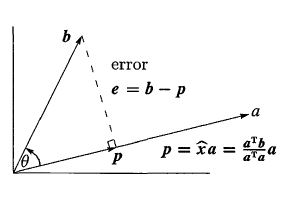
\includegraphics[width=10cm]{week5/projection_line}
\caption{The projection of $\bm b$ onto a line $\bm a$.}
\label{Fig:6:3}
\end{figure}
More generally, we can write the projection of $\bm b$ onto the line $\Span\{\bm a\}$ as:
\[
\Proj_{\Span\{\bm a\}}(\bm b)=\frac{\inp{\bm a}{\bm b}}{\inp{\bm a}{\bm a}}\bm a
\]
\paragraph{Changing an Orthogonal Basis}
Note that the error $\bm b-\Proj_{\Span\{\bm a\}}(\bm b)$ is perpendicular to $\bm a$, and $\bm b-\Proj_{\Span\{\bm a\}}(\bm b)\in\Span\{\bm a,\bm b\}.$

If we define $\bm b'=\bm b-\Proj_{\Span\{\bm a\}}(\bm b)$, then it's easy to check that $\Span\{\bm a,\bm b'\}=\Span\{\bm a,\bm b\}$ and $\bm a\perp\bm b'$. 

Hence, we convert the basis $\{\bm a,\bm b\}$ into another basis $\{\bm a,\bm b'\}$ such that the elements are orthogonal to each other. For general subspace we could also use this approach to obtain an orthogonal basis, which will be discussed in next lecture. 
\end{itemize}









%\section{Friday}\index{week7_Thursday_lecture}

\subsection{Polynomials}
\begin{definition}[polynomial]
Let $k$ be a field, and $f=\sum_{i=0}^nc_ix^i$ be a polynomial in $k[x]$. An element $a\in k$ is a root of $f$ if
\[
f(a)=\sum_{i=0}^nc_ia^i=0
\]
in $k$.
\end{definition}
question: what is $k[x]$?
\begin{corollary}
For all $f\in k[x]$, $a\in k$, then there exists $q\in k[x]$ such that
\[
f=q(x-a)+f(a)
\]
\end{corollary}
\begin{proof}
By division theorem, there exists $q,r\in k[x]$ such that
\[
f=q\cdot (x-a)+r,\quad
\mbox{deg}r<\mbox{deg}(x-a)=1
\]
which implies $r$ is a constant. Evaluate both sides for $x=a$, we have
\[
f(a)=r.
\]
\end{proof}
\begin{proposition}[root theorem]
Let $k$ be a field, $f$ a polynomial is $k[x]$. Then $a\in k$ is a root of $f$ iff $(x-a)$ divides $f$ in $k[x]$.
\end{proposition}
\begin{proof}
For forward direction, there exists $q\in k[x]$ such that
\[
f=q(x-a)+f(a)=q(x-a)\implies (x-a)|f
\]
For the reverse direction, if $f=q(x-a)$ for some $q\in k[x]$, then $f(a)=q(a)(a-a)=0$, i.e., $a$ is a root of $f$.
\end{proof}
\begin{theorem}
Let $k$ be a field, $f$ a nonzero polynomial in $k[x]$
\begin{enumerate}
\item
If $f$ has some degree $n$, then it has at most $n$ roots in $k$
\item
If $f$ has degree $n$ and $a_1,\dots,a_n\in k$ are distinct roots of $f$, then
\[
f=c\prod_{i=1}^n(x-a_i)
\]
for some $c\in k$.
\end{enumerate}
\end{theorem}
\begin{proof}
\begin{enumerate}
\item
We show the first part by induction. Suppose it holds for all nonzero polynomails with degree strictly less than $n$, and $\mbox{deg}f=n$. If $f$ has no roots in $k$, the proof is complete, otherwise suppose a root $a\in k$. There exists $q\in k[x]$ such that
\[
f=q(x-a)
\]
For the any other root $b\in k$, we have 
\[
0=q(b)(b-a)
\]
Since $k$ is a firld, it has no zero divisors, which implies $q(b)=0$, since $b-a\ne0$. Thus $b$ is a root of $q$. Since $\mbox{deg}q<n$, by induction we imply $q$ has at most $n-1$ roots, i.e., $f$ has at most $n-1$ roots that are different from $a$.
\item
If $n=1$, then $f=c_0+c_1x$ for some $c_i\in k$ with $c_1\ne0$, which implies
\[
0=f(a_1)=c_0+c_1a_1\implies c_0=-c_1a_1\implies
f=-c_1a_1+c_1x=c_1(x-a_1)
\]
Suppose $n>1$, and the claim holds for all $n'\in\mathbb{N}$ such that $n'<n$. By previuos claim, there exists $q\in k[x]$ such that
\[
f=q(x-a_n)
\]
Since $\mbox{deg}q=n-1$, and for $1\le i<n$, we have
\[
0=f(a_i)=q(a_i)(a_i-a_n)\implies q(a_i=0),
\]
which implies $a_1,\dots,a_{n-1}$ are $n-1$ distinct roots of $q$ as well. Thus there exists $c\in k$ s.t.
\[
q=c(x-a_1)\cdots(x-a_{n-1}),
\]
which follows that
\[
f=q(x-a_n)=c(x-a_1)\cdots(x-a_n)
\]
\end{enumerate}
\end{proof}

\begin{corollary}
Let $k$ be a field. Let $f,g$ be nonzero polynomails in $k[x]$. Let $n=\max\{\mbox{deg}f,\mbox{deg}g\}$. If $f(a)=g(a)$ for $n+1$ distinct $a\in k$, then $f=g$.
\end{corollary}
\begin{proof}
Let $h=f-g$, then $\mbox{deg}h\le n$. There are $n+1$ distinct elements $a\in k$ s.t. $h(a)=0$. If $h\ne0$, then it is a nonzero polynomial of degree $\le n$ which has $n+1$ distinct roots, which is a constraction. $h=0$ implies $f=g$.
\end{proof}
\begin{definition}
A polynomail in $k[x]$ is called a \emph{monic polynomial} if its leading coefficient is $1$.
\end{definition}
\begin{theorem}
Let $k$ be a field, then the ring $k[x]$ is a PID.
\end{theorem}
\begin{corollary}
Let $k$ be a field, and $f,g$ be nonzero polynomials in $k[x]$. There exists a unique monic polynomial $d\in k[x]$ with the following properties:
\begin{enumerate}
\item
$(f,g)=(d)$
\item
$d$ divides both $f$ and $g$, i.e., there exists $a,b\in k[x]$ s.t. $f=ad,g=bd$
\item
There are polynomials $p,q\in k[x]$ such that $d=pf+qg$
\item
If $h\in k[x]$ is a divisor of $f,g$, then $h$ divides $d$.	
\end{enumerate}
This $d\in k[x]$ is called the \emph{greatest common divisor} (GCD) of $f$ and $g$. We say $f$ and $g$ are \emph{relatively prime} if their GCD is 1.
\end{corollary}
\begin{proof}
By the PID theorem, there exists $d=\sum_{n=0}^\infty a_ix^i\in k[x]$ such that $(d)=(f,g)$. Replacing $d$ with $a_n^{-1}d$, we assume $d$ is a monic polynomial. It remains to show that $d$ is unique. 

Suppose $(d)=(d')$, there exists nonzero $p,q\in k[x]$ such that
\[
d'=pd,\quad
d=qd'
\]
which follows that
\[
\mbox{deg}d'=\mbox{deg}d+\mbox{deg}p,\quad
\mbox{deg}d=\mbox{deg}q+\mbox{deg}d'=\mbox{deg}q+\mbox{deg}d+\mbox{deg}p,
\]
i.e., $\mbox{deg}p=\mbox{deg}q=0$. Thus $\mbox{deg}d=\mbox{deg}d'$. Comparing the leading coefficients of $d'$ and $pd$, we have $p=1$, i.e., $d=d'$.

The remaining part follows similarly.
\end{proof}
\begin{definition}[Irreducible]
Let $R$ be a commutative ring. A non-zero element $p\in R$ which is not a unit is said to be \emph{irreducible} if $p=ab$ implies that either $a$ or $b$ is a unit.
\end{definition}
\begin{example}
The set of irreducible elements in the ring $\mathbb{Z}$ is
\[
\{\pm p\mid p\mbox{ is a prime number}\}
\]
\end{example}
Let $k$ be a field.
\begin{proposition}
A polynomial $f\in k[x]$ is a unit iff it is a \emph{nonzero} constant polynomial.
\end{proposition}
\begin{proposition}
A nonzero nonconstant polynoimial $p\in k[x]$ is \emph{irreducible} iff there is no $f,g\in k[x]$ with $\mbox{deg}f,\mbox{deg}g<\mbox{deg}p$, such that $fg=p$.
\end{proposition}
\begin{proof}
\begin{enumerate}
\item
Suppose $p$ is irreducible, and $p=fg$ for some $f,g\in k[x]$ such that $\mbox{deg}f,\mbox{deg}g<\mbox{deg}p$. Then $p=fg$ implies that $\mbox{deg}f,\mbox{deg}g$ are both positive. By previous lemma, both $f,g$ are non-units, which is a contradiction.
\item
Conversely, suppose $p$ is a nonzero non-unit in $k[x]$, which is not equal to $fg$ for $\forall f,g\in k[x]$ with $\mbox{deg}f,\mbox{deg}g<\mbox{deg}p$. Then $p=ab$ for $a,b\in k[x]$ implies that either $a$ or $b$ must have the same degree as $p$, and the otehr factor must be a nonzero constant, i.e., a unit in $k[x]$. Thus $p$ is irreducible.
\end{enumerate}
\end{proof}

\begin{proposition}[Euclid's Lemma]
Let $k$ be a field. Let $f,g$ be polynomials in $k[x]$. Let $p$ be an irreducible polynomial in $k[x]$. If $p|fg$ in $k[x]$, then $p|f$ or $p|g$.
\end{proposition}
\begin{proof}
Suppose $p$ not divides $f$, then any \emph{common divisor} of $p$ and $f$ must have degree strictly less than $\mbox{deg}p$. Since $p$ is irreducible, this implies that any common divisor of $p$ and $f$ is a nonzero constant. Thus the GCD of $p$ and $f$ is 1. There exists $a,b\in k[x]$ such that
\[
ap+bf=1\implies
apg+bfg=g
\]
Since $p$ divides the LHS, it also divides the RHS.
\end{proof}
\begin{proposition}
If $f,g\in k[x]$ are relatively prime, and both divide $h\in k[x]$, then $fg|h$.
\end{proposition}
question
\begin{theorem}[Unique Factorization]
Let $k$ be a field. Every non-constant polynomial $f\in k[x]$ may be written as
\[
f=cp_1\cdots p_n
\]
where $c$ is a non-zero constant, and each $p_i$ is a monic irreducible polynomials in $k[x]$. The factorization is \emph{unique} up to the ordering of the factors.
\end{theorem}
\begin{proof}
Similar to the proof of unique factorization for $\mathbb{Z}$
\end{proof}
\begin{theorem}
Let $k$ be a field, $p$ be a polynomial in $k[x]$. The following statements are equivalent:
\begin{enumerate}
\item
$k[x]/(p)$ is a field
\item
$k[x]/(p)$ is an integral domain
\item
$p$ is irreducible in $k[x]$.
\end{enumerate}
\end{theorem}
\begin{proof}
\begin{enumerate}
\item
(2) implies (3): If $p$ is not irreducible, then there exists $f,g\in k[x]$ with degree strictly less than that of $p$, such that $p=fg$.

It's clear that $p$ does not divide $f$ or $g$ in $k[x]$. The equivalence classes $\bar f$ and $\bar g$ of $f$ and $g$, respectively, modulo $(p)$ is not equal to zero in $k[x]/(p)$. (question) On the other hand, $\bar f\cdot\bar g=\bar{fg}=\bar p=0$ in $k[x]/(p)$, which implies that $k[x]/(p)$ is not an integral domain, which is a contradction.
\item
(3) implies (1): By definiton, the multiplicative identity $1$ of a field is different from addictive identity $0$. We first check that the equivalence lcass $1\in k[x]$ in $k[x]/(p)$ is not zero. Since $p$ is irreducible, we have $\mbox{deg}p>0$, and $1\notin(p)$. Therefore $1+(p)\ne 0+(p)$ in $k[x]/(p)$.

Next, we need to show the existence of multiplicative inverse of any nonzero element in $k[x]/(p)$. Given any $f\in k[x]$ whose equivalence $\bar f$ modulo $(p)$ is nonzero in $k[x]/(p)$, we want to constracut $\bar{f}^{-1}$. Since $\bar{f}\ne0$ in $k[x]/(p)$, we have $f-0\notin(p)$, i.e., $p$ does not divide $f$. Since $p$ is irreducible, we have $gcd(p,f)=1$. There exists $g,h\in k[x]$ such that $fg+hp=1$. Thus $\bar{f}^{-1}=\bar{g}$. This is becasue $fg-1=hp$ implies $fg-1\in(p)$, i.e., $\bar{f}\bar{g}=\bar{fg}=1$ in $k[x]/(p)$.


\end{enumerate}
\end{proof}
\subsection{Polynomials over $\mathbb{Z}$ and $\mathbb{Q}$}
\begin{theorem}
Let $f=a_0+a_1x+\cdots+a_nx^n$ be a polynomial in $\mathbb{Q}[x]$, with $a_i\in\mathbb{Z}$. Every rational root $r$ of $f$ in $\mathbb{Q}$ has the form $r=b/c$ $(b,c\in\mathbb{Z})$, where $b|a_0$ and $c|a_n$
\end{theorem}
\begin{proof}
Let $r=b/c$ be a rational root of $f$, where $b,c$ are relatively prime integers. We have
\[
0=\sum_{i=1}^na_i(b/c)^i
\]
Multiplying both sides above equation by $c^n$, we have
\[
0=a_0c^n+a_1c^{n-1}b+\cdots+a_nb^n
\]
or equivalently,
\[
a_0c^n=-(a_1c^{n-1}+\cdots+a_nb^n)
\]
Since $b$ divides the RHS, and $b,c$ are relatively prime, $b$ must divide $a_0$. Similarly,
\[
a_nb^n=-(a_0c^n+\cdots+a_{n-1}cb^{n-1})
\]
It is clear that $c$ divides $a_n$.
\end{proof}
\begin{definition}
A polynomial $f\in\mathbb{Z}[x]$ is said to be \emph{primitive} if the gcd of its coefficients is 1.
\end{definition}
\begin{remark}
Note that if $f$ is monic, i.e., its leading coefficient is 1, then it is primitive. If $d$ is the gcd of the coefficients of $f$, then $\frac{1}{d}f$ is a primitive polynomial in $\mathbb{Z}[x]$.
\end{remark}
\begin{theorem}[Gauss's Lemma]
If $f,g$ are both primitive, then $fg$ is primitive.
\end{theorem}
\begin{proof}
Write $f=\sum_{k=0}^ma_kx^k$ and $g=\sum_{k=0}^nb_kx^k$, then $fg=\sum_{k=0}^{m+n}c_kx^k$, where
\[
c_{k}=\sum_{i+j=k}a_ib_j.
\]
Assume that $fg$ is not primitive, then there exists a prime $p$ such that $p$ divides $c_k$ for $k=0,1,\dots,m+n$. Since $f$ is primitive, there exists smallest $u$ s.t. $a_u$ is not dividible by $p$; similarly, a smallest $v$ s.t. $b_v$ is not divisible by $p$. We have
\[
c_{u+v}=\left(\sum_{i+j=u+v,(i,j)\ne(u,v)}a_ib_j\right)+a_ub_v,
\]
which implies that
\[
a_ub_v=c_{u+v}-
\left(\sum_{i+j=u+v,i<u}a_ib_j\right)
-
\left(\sum_{i+j=u+v,i>u}a_ib_j\right)
\]
By the minimum conditons on $u$ and $v$, each term on the RHS of the above equation is divisible by $p$. Thus $p$ divides $a_u$ and $b_v$, which implies that $p$ divides either $a_u$ or $b_v$, which is a contradiction.
\end{proof}
\begin{proposition}
Every nonzero $f\in\mathbb{Q}[x]$ has a unique factorization:
\[
f=c(f)f_0,
\]
where $c(f)$ is a positive rational number, and $f_0$ is a primitive polynomial in $\mathbb{Z}[x]$.
\end{proposition}
\begin{definition}
The rational number $c(f)$ is called the \emph{content} of $f$.
\end{definition}















%\section{Assignment Four}\index{Assignment_Four}
\begin{enumerate}
\item
Let
\[
\bm A=\begin{bmatrix}
1&2&3&1&-3\\2&5&5&4&9\\3&7&8&5&6
\end{bmatrix}
\]
\begin{enumerate}
\item
Compute the \textit{reduced row echelon form} $\bm U$ of $\bm A$.
\item
Compute all solutions of $\bm{Ax}=\bm b$, where $\bm b=\begin{bmatrix}
1&1&2
\end{bmatrix}\trans.$
\item
Compute all solutions of $\bm{Ax}=\bm b$, where $\bm b=\begin{bmatrix}
b_1&b_2&b_3
\end{bmatrix}\trans.$\\
Note:Identify when there is \textit{no solution}, and when the solution \textit{exists}, write down all solutions in terms of $b_1,b_2,b_3$.
\end{enumerate}
\item
In each of the following, determine the \textit{dimension} of the space:
\begin{enumerate}
\item
$\Span\left\{
\begin{pmatrix}
1\\-2\\2
\end{pmatrix},\begin{pmatrix}
2\\-2\\4
\end{pmatrix},\begin{pmatrix}
-3\\3\\6
\end{pmatrix}
\right\};$
\item
$\col(\bm A)$, where $\bm A=\begin{bmatrix}
1&-2&3&2\\-1&2&-2&-1\\2&-4&5&3
\end{bmatrix};$
\item
$N(\bm B)$, where $\bm B=\begin{bmatrix}
1&3&2\\2&1&4\\4&7&8
\end{bmatrix};$
\item
$\Span\{(x-2)(x+2),x^2(x^4-2),x^6-8\};$
\item
$\Span\{5,\cos 2x,\cos^2 x\}$ as a \textit{subspace} of $C[-\pi,\pi].$\\
$C[-\pi,\pi]$ denotes the space of \textit{continuous functions defined on the domain $C[-\pi,\pi].$}
\end{enumerate}
\item
Let $\bm A$ be an $6\x n$ matrix of rank $r$. For each pair of values of $r$ and $n$ below, how many solutions could one have for the linear system $\bm{Ax}=\bm b$? Explain your answers.
\begin{enumerate}
\item
$n=7,r=5;$
\item
$n=7,r=6;$
\item
$n=5,r=5.$
\end{enumerate}
\item
Prove the following proposition:\\
Let $\bm V$ be a vector space of dimension $n>0$, then
\begin{enumerate}
\item
Any set of n \textit{linearly independent} vectors in $\bm V$ form a basis.
\item
Any set of $n$ vectors that span $\bm V$ form a basis.
\end{enumerate}
\textit{Hint: refer to theorem(\ref{theorem_3.3})}
\item
\begin{enumerate}
\item
Assume $\bm U.\bm V$ are subspaces of a vector space $\bm W$.\\
Define $\bm U+\bm V=\{u+v|u\in\bm U,v\in\bm V\}$, i.e. each vector in $\bm U+\bm V$ is the sum of one vector in $\bm U$ and one vector in $\bm V$.\\
Prove that $\bm U+\bm V$ is a subspace of $\bm W$.
\item
Prove the intersection $\bm U\cap\bm V=\{x|x\in\bm U\text{ and }x\in\bm V\}$ is also a subspace of $\bm W.$
\item
In $\mathbb{R}^4$, let $\bm U$ be the subspace of all vectors of the form $\begin{bmatrix}
u_1&u_2&0&0
\end{bmatrix}\trans$, and let $\bm V$ be the subspace of all vectors of the form $\begin{bmatrix}
0&v_2&v_3&0
\end{bmatrix}\trans.$ What are the dimensions of $\bm U,\bm V,\bm U\cap\bm V,\bm U+\bm V$?
\item
If $\bm U\cap\bm V=\{\bm0\}$, prove that $\dim(\bm U+\bm V)=\dim(\bm U)+\dim(\bm V).$
\end{enumerate}
\item
Let $\bm A$ and $\bm B$ be $m\x n$ matrices. Prove that 
\[
\rank(\bm A+\bm B)\le\rank(\bm A)+\rank(\bm B).
\]
\item
Let $\bm A\in\mathbb{R}^{m\x n}$ is an arbitrary matrix, $\bm B\in\mathbb{R}^{n\x n}$ is a square matrix. Prove that
\begin{enumerate}
\item
$\rank(\bm{AB})\le\rank(\bm A);$
\item
If $\rank(\bm B)=n$, then $\rank(\bm{AB})=\rank(\bm A).$
\end{enumerate}
\item
Prove that any $(n-1)$ vectors in $\mathbb{R}^n$ cannot form a basis.\\
Note: this is a corollary of theorem$(\ref{theorem_3.2})$. You should prove it by assuming theorem$(\ref{theorem_3.2})$ is unknown. You may check the proposition$(\ref{solution_for_undetermined_system})$ as hint.
\end{enumerate}
%%
\chapter{Week4}

\section{Convergence}\index{week4_Friday_lecture}

\begin{definition}[Convergent]
An infinite sequence $\{z_n\}$ of complex numbers has a limit $z_0$, if for $\forall$ $\varepsilon>0$, there exists a positive integer $n_0$ such that
\[
\begin{array}{ll}
|z_n-z|<\varepsilon,
&
\mbox{whenever }n>n_0
\end{array}
\]
We say the sequence $z_n$ converges to $z$ and write as
\[
\lim_{n\to\infty}z_n=z
\]
When the sequence does not have a limit, then it diverges.
\end{definition}
The uniqueness of limit of a seuqnece is guaranteed.

\begin{proposition}
For $z_n=x_n+iy_n$, we have 
\[
\lim_{n\to\infty}z_n=x+iy
\]
if and only if
\[
\begin{array}{lll}
\lim_{n\to\infty}x_n=x,
&
\mbox{and}
&
\lim_{n\to\infty}y_n=y
\end{array}
\]
\end{proposition}

\begin{definition}[Convergent Series]
An infinite \emph{series} $\sum_{n=1}^\infty z_n$ of complex numbers converges to the sum $S$ if the partial sum sequences
\[
S_N=\sum_{n=1}^Nz_n
\]
converges to $S$, then we write
\[
\sum_{n=1}^\infty z_n=S.
\]
\end{definition}

\begin{proposition}
For $z_n=x_n+iy_n$, we have 
\[
\sum_{n=1}^\infty z_n=X+iY
\]
if and only if
\[
\begin{array}{lll}
\sum_{n=1}^\infty x_n=X
&
\mbox{and}
&
\sum_{n=1}^\infty y_n=Y
\end{array}
\]
\end{proposition}

\begin{proposition}
The series $\sum_{n=1}^\infty z_n$ converges implies that $\lim_{n\to\infty}z_n=0$.
\end{proposition}

\begin{definition}[Absolute Convergence]
The series $\sum_{n=1}^\infty z_n$ is said to be \emph{absolutely convergent} if
\[
\sum_{n=1}^\infty|z_n|
\]
converges, i.e., $\sum_{n=1}^\infty|x_n|$ and $\sum_{n=1}^\infty|y_n|$ converge.
\end{definition}
\begin{proposition}
Absolute convergence implies convergence
\end{proposition}

\begin{definition}[Remainder]
The \emph{remainder} $\rho_N$ of a series after $N$ terms is defined by:
\[
\rho_N=\sum_{n=N+1}^\infty S_n
\]
\end{definition}
\begin{proposition}
A series converges to a number $S$ iff the sequence of remainders tends to zero.
\end{proposition}

It's easy to verifty that
\[
\sum_{n=0}^\infty z_n=\frac{1}{1-z},\qquad\mbox{whenever }|z|<1
\]
with the aid of partial sums and remainders.

\subsection{Taylor Series}
\begin{definition}[Power Series]
The power series has the form
\[
\sum_{n=0}^\infty a_n(z-z_0)^n
\]
\end{definition}

\begin{theorem}[Convergent of Taylor Series]
Suppose $f$ is \emph{analytic} on $|z-z_0|<R$, then 
\begin{equation}
f(z)=\sum_{n=0}^\infty \frac{f^{(n)}(z_0)}{n!}(z-z_0)^n,
\end{equation}
for $|z-z_0|<R$, i.e., $f(z)$ admits its Taylor expansion at $z=z_0$ in this rigion.
\end{theorem}
\begin{remark}
Typically, when $z_0=0$, we say this series is the \emph{Maclaurin series}.
\end{remark}
\begin{proof}
\textbf{Step 1: Applying Cauchy Integral Formula.}
For fixed $z$, let $r:=|z-z_0|<R$ and take $r_0$ such that $r<r_0<R$. Construct a contour $C_0:\{z\in\mathbb{C}\mid |z-z_0|=r_0\}$ in the positive sense, which follows that
\begin{subequations}
\begin{align}
f(z)&=\frac{1}{2\pi i}\int_{C_0}\frac{f(s)}{s-z}\diff s\label{Eq:4:2:b}
\end{align}

\textbf{Step 2: Expand $1/(s-z)$.} With some calculation, we obtain
\begin{align}\label{Eq:4:2}
\frac{1}{s-z}&=\frac{1}{s-z_0}\cdot\frac{1}{1-\frac{z-z_0}{s-z_0}}\\
&=\frac{1}{s-z_0}\left\{1+\frac{z-z_0}{s-z_0}+\cdots+(\frac{z-z_0}{s-z_0})^{N-1}+\frac{(\frac{z-z_0}{s-z_0})^{N}}{1 - \frac{z-z_0}{s-z_0}}\right\}\label{Eq:4:2:d}\\
&=\frac{1}{s-z_0}+\frac{z-z_0}{(s-z_0)^2}+\cdots+\frac{(z-z_0)^{N-1}}{(s-z_0)^N}+\frac{(z-z_0)^N}{(s-z)(s-z_0)^N}\label{Eq:4:2:e}
\end{align}
where $(\ref{Eq:4:2:d})$ is because that
\[
\frac{1}{1-c}=1+c+c^2+\cdots+c^{N-1}+\frac{c^N}{1-c}. 
\]
Substituting (\ref{Eq:4:2:e}) into (\ref{Eq:4:2:b}), we obtain
\begin{align*}
f(z)&=\frac{1}{2\pi i}\int_{C_0}\left\{\frac{f(s)}{(s-z_0)}+\frac{f(s)(z-z_0)}{(s-z_0)^2}+\cdots+\frac{f(s)(z-z_0)^{N-1}}{(s-z_0)^N}+\frac{f(s)(z-z_0)^N}{(s-z)(s-z_0)^N}
\right\}\\
&=f(z_0)+f'(z_0)(z-z_0)+\cdots+\frac{f^{(N-1)}(z_0)}{(N-1)!}(z-z_0)^{N-1}+\rho_N(z)
\end{align*}
with
\begin{equation}\label{Eq:4:2:e}
\rho_N(z)=\frac{(z-z_0)^B}{2\pi i}\int_{C_0}\frac{f(s)}{(s-z)(s-z_0)^N}\diff s
\end{equation}

\textbf{Step 3: Show that $\rho_N(z)$ is convergent.}
\begin{align}
|\rho_N(z)|&\le\frac{|z-z_0|^N}{2\pi}\int_{C_0}\frac{|f(s)|}{|s-z||s-z_0|^N}|\diff s|\\
&\le\frac{r^N}{2\pi}\int_{C_0}\frac{M}{(r_0-r)r_0^N}|\diff s|\\
&=\frac{Mr_0}{r_0-r}\left(\frac{r}{r_0}\right)^N
\end{align}
where we suppose $|f(s)|\le M$ on $C_0$; and $|s-z|\ge|s-z_0| - |z-z_0| = r_0-r$. Therefore,
\[
\rho_N(z)\to0
\]
since $r<r_0$ and $(r/r_0)^N\to0$.
\end{subequations}




\end{proof}

\begin{example}
\begin{enumerate}
\item
For $f(z)=e^z$, which is analytic for $|z-0|<\infty$, thus we have
\[
e^z=\sum_{n=0}^\infty\frac{z^n}{n!},\qquad |z|<\infty
\]
\item
For $f(z)=\sin z=\frac{e^{iz} - e^{-i}}{2i}$, which is analytic for $|z-0|<\infty$, thus we have $f^{(2n)}(0)=0; f^{(2n+1)}(0)=(-1)^n$, and therefore
\[
\sin z=\sum_{n=0}^\infty\frac{(-1)^n}{(2n+1)!}z^{2n+1},\qquad |z|<\infty
\]
\item
For $f(z)=\frac{1}{1-z}$, which is analytic for $|z-0|<1$, we have $f^{(0)}=n!$, and therefore
\[
\frac{1}{1-z}=\sum_{n=0}^\infty\frac{n!}{n!}z^n=\sum_{n=0}^\infty z^n,\qquad |z|<1
\]
\item
For $f(z)=\frac{1}{z}\cdot\frac{1}{1+z}$, we have
\[
\frac{1}{1+z}=\sum_{n=0}^\infty(-z)^n,\qquad |z|<1,
\]
and therefore
\[
\frac{1}{z+z^2}=\frac{1}{z}+\sum_{n=1}^\infty(-1)^nz^{n-1},\qquad 0<|z|<1
\]
\end{enumerate}
\end{example}
\subsection{Laurent Series}
We cannot apply Taylor expansion at a non-analytic point. Fortunately, we can find another series representation for $f(z)$ that involving positive and negative powers of $(z-z_0)$
\begin{definition}[Laurent Series]
The \emph{Laurent series} has the form
\[
\sum_{n=0}^\infty a_n(z-z_0)^n+\sum_{n=1}^\infty\frac{b_n}{(z-z_0)^n}
\]
\end{definition}
\begin{theorem}
Suppose $f$ is analytic throughout an \emph{annular domain} $R_1<|z-z_0|<R_2$. Let $C$ be any \emph{positively oriented simple closed contour} around $z_0$ and lying in that domain. Then
\begin{subequations}
\begin{equation}
f(z)=\sum_{n=0}^\infty a_n(z-z_0)^n+\sum_{n=1}^\infty\frac{b_n}{(z-z_0)^n},\qquad
R_1<|z-z_0|<R_2
\end{equation}
with
\begin{align}
a_n&=\frac{1}{2\pi i}\int_C\frac{f(z)}{(z-z_0)^{n+1}}\diff z,\qquad n=0,1,2,\dots\\
b_n&=\frac{1}{2\pi i}\int_C\frac{f(z)}{(z-z_0)^{-n+1}}\diff z,\qquad n=1,2,\dots
\end{align}
\end{subequations}

\end{theorem}
\begin{remark}
The Laurent series is often written as the form
\[
f(z)=\sum_{n=-\infty}^\infty c_n(z-z_0)^n,\qquad R_1<|z-z_0|<R_2,
\]
where
\[
c_n=\frac{1}{2\pi i}\int_C\frac{f(z)}{(z-z_0)^{n+1}}\diff z,\qquad n=0,\pm1,\pm2,\dots
\]
When $f$ is analytic on $|z-z_0|<R_2$, we have $b_n=0,a_n=\frac{f^{(n)}(z_0)}{n!}$, i.e., the Laurent series reduces to the Taylor series.
\end{remark}
\begin{proof}
\begin{itemize}
\item
For fixed $z$ in the domain, let $r=|z-z_0|$, and construct two positively oriented contours $C_i:\{z\in\mathbb{C}\mid|z-z_0|=r_i\},i=1,2$ such that $R_1<r_1<r<r_2<R_2$. (The reaon why we don't use the boundary is that the function is not analytic on the boundary but only interior to)
\item
Construct a circle $\gamma:\{s\in\mathbb{C}\mid s = z + \delta e^{i\theta},0\le\theta\le2\pi\}$, where the $\delta$ is picked such that $\gamma$ is contained in the interior between $C_1,C_2$. By Cauchy Integral Formula,
\begin{equation}
\int_{C_2}\frac{f(s)\diff s}{s-z}=\int_{C_1}\frac{f(s)\diff s}{s-z}+\int_{\gamma}\frac{f(s)\diff s}{s-z}
\end{equation}
Or equivalently,
\[
f(z)=\frac{1}{2\pi i}\int_{C_2}\frac{f(s)\diff s}{s-z}+\frac{1}{2\pi i}\int_{C_1}\frac{f(s)\diff s}{z-s}
\]
\item
By applying the same trick as (\ref{Eq:4:2}), we have
\begin{subequations}
\begin{equation}
f(z)=\sum_{n=0}^{N-1}a_n(z-z_0)^n+\rho_N(z)+\sum_{n=1}^N\frac{b_n}{(z-z_0)^n}+\sigma_N(z)
\end{equation}
with
\begin{align}
a_n&=\frac{1}{2\pi i}\int_{C_2}\frac{f(s)\diff s}{(s-z_0)^{n+1}}\\
b_n&=\frac{1}{2\pi i}\int_{C_1}\frac{f(s)\diff s}{(s-z_0)^{-n+1}}\\
\rho_N(z)&=\frac{(z-z_0)^N}{2\pi i}\int_{C_2}\frac{f(s)\diff s}{(s-z)(s-z_0)^N}\\
\sigma_N(z)&=\frac{(z-z_0)^{-N}}{2\pi i}\int_{C_1}\frac{f(s)\diff s}{(z-s)(s-z_0)^{-N}}
\end{align}
\end{subequations}
\item
Then we bound the term $\rho_N(z)$ and $\sigma_N(z)$. Suppose $|f(s)|\le M$ on $C_1,C_2$, and note that $|s-z|\ge r_2-r$ for $s\in C_2$; $|z-s|\ge r-r_1$ for $s\in C_1$:
\begin{align*}
\rho_N(z)&\le\frac{Mr_2}{r_2-r}\left(\frac{r}{r_2}\right)^N\\
\sigma_N(z)&\le\frac{Mr_1}{r-r_1}\left(\frac{r_1}{r}\right)^N
\end{align*}
\item
Finally, note that
\begin{align*}
a_n&=\frac{1}{2\pi i}\int_{C}\frac{f(s)\diff s}{(s-z_0)^{n+1}}\\
b_n&=\frac{1}{2\pi i}\int_{C}\frac{f(s)\diff s}{(s-z_0)^{-n+1}}\\
\end{align*}





\end{itemize}
\end{proof}

\begin{example}
\begin{enumerate}
\item
\[
f(z)=\frac{1}{z-1} - \frac{1}{z-2}
\]
This function has two singular points $1,2$. We take $z_0=0$.
\begin{itemize}
\item
When $z\in D_1=\{z:|z|<1\}$, we obtain the Taylor expansion:
\[
f(z)=-\sum_{n=0}^\infty z^n+\sum_{n=0}^\infty\frac{z^n}{2^{n+1}}=\sum_{n=0}^\infty(2^{-n-1}-1)z^n
\]
\item
When $z\in D_2=\{z:1<|z|<2\}$, we obtain the Laurent series:
\[
f(z)=\sum_{n=0}^\infty\frac{z^n}{2^{n+1}}+\sum_{n=1}^\infty\frac{1}{z^n}
\]
\item
When $z\in D_3=\{z:|z|>2\}$, we obtain
\[
f(z)=\sum_{n=1}^\infty\frac{1-2^{n-1}}{z^n}
\]
\end{itemize}
\item
Expand $f(z)=\frac{-z}{(z-1)(z-3)}$ near $z_0=1$, and find the domain of expansion.

The expansion should be the laurent series with domain of expansion $0<|z-1|<2$.
\[
f(z)=\frac{1/2}{z-1}-\frac{3/2}{z-3}=\frac{1/2}{z-1}+\sum_{n=0}^\infty\frac{3}{2^{n+2}}(z-1)^n
\]





\end{enumerate}
\end{example}
\subsection{Power Series}
For power series
\begin{equation}\label{Eq:4:6}
\sum_{n=0}^\infty a_n(z-z_0)^n
\end{equation}
, first we study the range of its convergence.
\begin{theorem}\label{The:4:3}
If the power series (\ref{Eq:4:6}) converges at $z=z_1(\ne z_0)$, then it is \emph{absolutely convergent} at each point in the disk $|z-z_0|<|z_1-z_0|$.
\end{theorem}
\begin{proof}
For any point $z$ around the disk, we have, we have
\[
\left|\frac{z-z_0}{z_1-z_0}\right|:=q<1,
\]
which follows that
\[
|a_n(z-z_0)^n|=|a_n(z_1-z_0)^n|\left|\frac{z-z_0}{z_1-z_0}\right|^n\le Mq^n,
\]
where $|a_n(z_1-z_0)^n|\le M$ since $z_1$ makes the series convergent. By Comparison test, we conclude (\ref{Eq:4:6}) is absolutely convergent.
\end{proof}
\begin{definition}[Uniform convergence]
The series (\ref{Eq:4:6}) is said to be \emph{uniformly convergent} for $|z-z_0|<R$ if as $N\to\infty$,
\[
\sup_{|z-z_0|<R}|\rho_N(z)|\to0
\]
\end{definition}

\begin{theorem}
If the power series (\ref{Eq:4:6}) converges at $z=z_1(\ne z_0)$, then it must be uniformly convergent for any closed circle $|z-z_0|\le \rho$ ($\rho<|z_1-z_0|$).
\end{theorem}
\begin{proof}
Notice that for any $\rho<|z_1-z_0|$, for any $z$ in that closed circle, we have
\[
|a_n(z-z_0)^n|\le |a_n\rho^n|
\]
Due to the conclusion in Theorem(\ref{The:4:3}), we conclude $\sum_{n=1}^\infty |a_n|\rho^n$ is convergent, and therefore $(\ref{Eq:4:6})$ is uniformly convergent.

\end{proof}
Now we are curious about whether the power series is analytic. First we show under which condition does the power series is continuous.
\begin{theorem}
The series (\ref{Eq:4:6}) represents a continuous function at each point inside the circle of convergence.
\end{theorem}

\begin{theorem}
The sum $S(z)$ of power series is analytic at each point $z$ interior to the circle convergence of that series.
\end{theorem}






















%%\include{week4/Lecture_2}
%
\chapter{Midterm}

\section{Sample Exam}\index{Sample Exam}
DURATION OF EXAMINATION: 2 hours in-class\\
\textit{This examination paper includes $6$ pages and $6$ problems. You are responsible for ensuring that
your copy of the paper is complete. Bring any discrepancy to the attention of your invigilator.}\\
\begin{enumerate}
\item \textbf{(30 points)} \textit{Solving a linear system of equations}\\
For a real number $c$, consider the linear system:
\begin{align}
x_1+x_2+cx_3+x_4&=c\\
-x_2+x_3+2x_4&=0\\
x_1+2x_2+x_3-x_4&=-c
\end{align}
do the following:
\begin{enumerate}
\item
Write out the \textit{coefficient matrix} of the system.\\
\item
Write out the \textit{augmented matrix} for this system and calculate its \textit{row-reduced echelon form.}\\
\item
Write out the complete set of solutions in \textit{vector form.}\\
\item
What is the \textit{rank} of the coefficient matrix $\bm A$? Justify your answer.\\
\item
Find a \textit{basis}  of the subspace of solutions when $c=0$.
\end{enumerate}
\newpage
\item \textbf{(20 points)} \textit{Vector space}\\
Find a \textit{basis} for each of the following spaces.
\begin{itemize}
\item
Space of $n\x n$ \textit{skew symmetric matrices} (i.e. those matrix satisfying $\bm A=-\bm A\trans$)\\
\item
The space of all \textit{polynomials} of the form $ax^2+bx+2a+3b$, where $a,b\in\mathbb{R}.$\\
\item
$\Span\{x-1,x+1,2x^2-2\}.$
\end{itemize}
\newpage
\item \textbf{(15 points)} \textit{Matrix multiplications}\\
Prove the following statements:
\begin{enumerate}
\item
Define the set of $n\x n$ \textit{diagonol matrices} to be $\kappa$. Prove that for a diagonal matrix $\bm D$ with \textit{distinct} elements (i.e. $\bm D_{ii}\ne\bm D_{jj},\forall i\ne j$), the set $\{\bm A\in\mathbb{R}^{n\x n}|\bm{AD}=\bm{DA}\}$ is exactly $\kappa$.\\
\item
If an $n\x n$ matrix $\bm A$ satisfies $\bm{AB}=\bm{BA}$ for any $n\x n$ matrix $\bm B$, then $\bm A$ must be of the form $c\bm I$, where $c$ is a scalar.
\end{enumerate}
\newpage
\item \textbf{(10 points)} \textit{Matrix Inverse}\\
\begin{enumerate}
\item
Compute the inverse of the matrix $\begin{pmatrix}
5&4\\4&5
\end{pmatrix}.$
\item
Compute the inverse of the matrix $\begin{pmatrix}
a&b\\c&d
\end{pmatrix}$ if exists. When does the inverse of the matrix exist?
\end{enumerate}
\newpage
\item \textbf{(15 points)} \textit{Matrix rank}\\
\begin{enumerate}
\item
Suppose $\bm u\in\mathbb{R}^{n\x 1}$ satisfies $\|\bm u\|=1$. What is the rank of the matrix $\bm I-\bm u\bm u\trans$?\\
\item
Suppose $\bm u\in\mathbb{R}^{n\x 1}$ satisfies $\|\bm u\|=1$. Define $\bm P=\bm I-\bm u\bm u\trans$. What is the rank of $\bm P^2$? What about $\bm P^5$?\\
\item
Suppose $\bm x,\bm y\in\mathbb{R}^{n\x 1}$. What is the rank of the matrix $\bm I-\bm x\bm y\trans$?\end{enumerate}
\newpage
\item \textbf{(20 points)} \\
State your answers. No justifications are required.
\begin{enumerate}
\item
We know $a^2-b^2=(a+b)(a-b)$, where $a,b\in\mathbb{R}$. When $\bm A,\bm B$ are square matrices, can we
represent $\bm A^2-\bm B^2$ by only $(\bm A+\bm B)(\bm A-\bm B)$?\\
\item
True or False: If $\bm A$ and $\bm B$ are \textit{invertible}, then $\bm A+\bm B$ is also \textit{invertible}.\\
\item
True or False: The set of all \textit{real-valued} functions on $\mathbb{R}$ such that $f(1)=0$ is a \textit{vector space}.\\
\item
True or False: The product of two \textit{invertible} $n\x n$ matrices is \textit{invertible}\\
\item
True or False: If two matrices have the same \textit{reduced row echelon form}, then they have the
same \textit{column space}.\\
\item
True or False: If two columns of the square $\bm A$ are the same, then $\bm A$ \textit{cannot} be invertible.\\
\item
True or False: For an $m\x n$ matrice $\bm A$, $\rank(\bm A)+\dim(\row(\bm A))=n.$
\end{enumerate}
\end{enumerate}
%\section{Midterm Exam}\index{Midterm Exam}
DURATION OF EXAMINATION: 2 hours in-class\\
\textit{This examination paper includes $6$ pages and $6$ problems. You are responsible for ensuring that
your copy of the paper is complete. Bring any discrepancy to the attention of your invigilator.}\\
\begin{enumerate}
\item \textbf{(30 points)} \textit{Solving a linear system of equations}\\
For the system
\begin{align}
x-y+3z&=1\\
y&=-2x+5\\
9z-x-5y+7&=0
\end{align}
do the following:
\begin{enumerate}
\item
Write the system in the matrix form
\[
\bm{Ax}=\bm b\text{ for }\bm x=\begin{pmatrix}
x\\y\\z
\end{pmatrix}.
\]
\item
Write out the \textit{augmented matrix} for this system and calculate its \textit{row-reduced echelon form}.\\
\item
Write out the complete set of solutions (if they exist) in \textit{vector form} using parameters if
needed.\\
\item
Calculate the \textit{inverse} of the \textit{coefficient matrix} $\bm A$ you found in part $(a)$, if it exists, or show that $\bm A^{-1}$ doesn't exist.\\
\item
What is the rank of matrix $\bm A$? Justify your answer.
\end{enumerate}


\newpage
\item \textbf{(20 points)} \textit{Vector space}\\
Let $V$ be the subspace of $\mathbb{R}^4$ given by all solutions to the equation $2x_1-x_2+3x_3=0.$
\begin{enumerate}
\item
Give the set of all solutions in terms of \textit{free variables}.\\
\item
What is the dimension of $V$? Justify your answer.\\
\item
Find a 4 by 3 matrix $\bm A$ such that the \textit{column space} of $\bm A$ is equal to $V$.\\
\item
Find a 1 by 4 matrix $\bm B$ such that the \textit{null space} of $\bm B$ is equal to $V$.\end{enumerate}





\newpage
\item \textbf{(15 points)} \textit{Matrix multiplications}\\
If possible, find 3 by 3 matrices $\bm B$ such that
\begin{enumerate}
\item
$\bm{BA}=2\bm A$ for every $\bm A$.\\
\item
$\bm{BA}=2\bm B$ for every $\bm A$.\\
\item
$\bm{BA}$ has the \textit{first} and \textit{last} rows of $\bm A$ reversed.\\
\item
$\bm{BA}$ has the \textit{first} and \textit{last} columns of $\bm A$ reversed.
\end{enumerate}




\newpage
\item \textbf{(10 points)} \textit{Matrix Inverse}\\
For an $m\x n$ matrix $\bm A$, we say an $n\x m$ matrix $\bm C$ is a \textit{right inverse} of $\bm A$ if $\bm{AC}=\bm I_m$, where $\bm I_m$ is the $m\x m$ identity matrix.
\begin{enumerate}
\item
Prove that $\bm A$ has a \textit{right inverse} if and only if $\bm{Ax}=\bm b$ has at least one solution for any $\bm b\in\mathbb{R}^m$. Prove that the rank of such $\bm A$ must be $m$.\\
\item
Compute a \textit{right inverse} of the following matrices (if exists):
\begin{gather*}
\bm A=\begin{pmatrix}
1&2&7\pi
\end{pmatrix}\\
\bm B=\begin{pmatrix}
1\\2\\7\pi
\end{pmatrix}
\end{gather*}
\end{enumerate}


\newpage
\item \textbf{(15 points)} \textit{Matrix rank}\\
\begin{enumerate}
\item
For a square matrix $\bm A$, is $\rank(\bm A\trans+\bm A)=\rank(\bm A)$ always true? Justify your answer.\\
\item
Prove that for any $m$ by $n$ matrix $\bm A$, the null space of $\bm A$ and the null space of $\bm A\trans\bm A$ are the same.\\
\item
Prove that for any $m$ by $n$ matrix $\bm A$, $\rank(\bm A\trans\bm A)=\rank(\bm A).$
\end{enumerate}



\newpage
\item \textbf{(20 points)} \\
State your answers. No justifications are required.
\begin{enumerate}
\item
If $\bm A=\bm A\trans$ and $\bm B=\bm B\trans$ which of these matrices are certainly \textit{symmetric}?
\begin{enumerate}
\item
$\bm A^2-\bm B^2$
\item
$(\bm A+\bm B)(\bm A-\bm B)$
\item
$\bm{ABA}$
\item
$\bm{ABAB}$
\end{enumerate}
\item
Let $\bm A$ be a $5\x 8$ matrix with rank equal to $5$ and let $\bm b$ be any vector in $\mathbb{R}^5$. How many solutions does this system have?\\
\item
True or False: If two $n\x n$ matrices $\bm A$ and $\bm B$ are both \textit{singular}, then $\bm A+\bm B$ is also \textit{singular}.\\
\item
True or False: The set of $n\x n$ matrices with rank no more than $r(r\le n)$ is a vector space.\\
\item
True or False: The set of all \textit{real-valued} functions on $\mathbb{R}$ such that $f(1)=1$ is a vector space.
\end{enumerate}
\end{enumerate}
%\section{Friday}\index{week7_Thursday_lecture}

\subsection{Polynomials}
\begin{definition}[polynomial]
Let $k$ be a field, and $f=\sum_{i=0}^nc_ix^i$ be a polynomial in $k[x]$. An element $a\in k$ is a root of $f$ if
\[
f(a)=\sum_{i=0}^nc_ia^i=0
\]
in $k$.
\end{definition}
question: what is $k[x]$?
\begin{corollary}
For all $f\in k[x]$, $a\in k$, then there exists $q\in k[x]$ such that
\[
f=q(x-a)+f(a)
\]
\end{corollary}
\begin{proof}
By division theorem, there exists $q,r\in k[x]$ such that
\[
f=q\cdot (x-a)+r,\quad
\mbox{deg}r<\mbox{deg}(x-a)=1
\]
which implies $r$ is a constant. Evaluate both sides for $x=a$, we have
\[
f(a)=r.
\]
\end{proof}
\begin{proposition}[root theorem]
Let $k$ be a field, $f$ a polynomial is $k[x]$. Then $a\in k$ is a root of $f$ iff $(x-a)$ divides $f$ in $k[x]$.
\end{proposition}
\begin{proof}
For forward direction, there exists $q\in k[x]$ such that
\[
f=q(x-a)+f(a)=q(x-a)\implies (x-a)|f
\]
For the reverse direction, if $f=q(x-a)$ for some $q\in k[x]$, then $f(a)=q(a)(a-a)=0$, i.e., $a$ is a root of $f$.
\end{proof}
\begin{theorem}
Let $k$ be a field, $f$ a nonzero polynomial in $k[x]$
\begin{enumerate}
\item
If $f$ has some degree $n$, then it has at most $n$ roots in $k$
\item
If $f$ has degree $n$ and $a_1,\dots,a_n\in k$ are distinct roots of $f$, then
\[
f=c\prod_{i=1}^n(x-a_i)
\]
for some $c\in k$.
\end{enumerate}
\end{theorem}
\begin{proof}
\begin{enumerate}
\item
We show the first part by induction. Suppose it holds for all nonzero polynomails with degree strictly less than $n$, and $\mbox{deg}f=n$. If $f$ has no roots in $k$, the proof is complete, otherwise suppose a root $a\in k$. There exists $q\in k[x]$ such that
\[
f=q(x-a)
\]
For the any other root $b\in k$, we have 
\[
0=q(b)(b-a)
\]
Since $k$ is a firld, it has no zero divisors, which implies $q(b)=0$, since $b-a\ne0$. Thus $b$ is a root of $q$. Since $\mbox{deg}q<n$, by induction we imply $q$ has at most $n-1$ roots, i.e., $f$ has at most $n-1$ roots that are different from $a$.
\item
If $n=1$, then $f=c_0+c_1x$ for some $c_i\in k$ with $c_1\ne0$, which implies
\[
0=f(a_1)=c_0+c_1a_1\implies c_0=-c_1a_1\implies
f=-c_1a_1+c_1x=c_1(x-a_1)
\]
Suppose $n>1$, and the claim holds for all $n'\in\mathbb{N}$ such that $n'<n$. By previuos claim, there exists $q\in k[x]$ such that
\[
f=q(x-a_n)
\]
Since $\mbox{deg}q=n-1$, and for $1\le i<n$, we have
\[
0=f(a_i)=q(a_i)(a_i-a_n)\implies q(a_i=0),
\]
which implies $a_1,\dots,a_{n-1}$ are $n-1$ distinct roots of $q$ as well. Thus there exists $c\in k$ s.t.
\[
q=c(x-a_1)\cdots(x-a_{n-1}),
\]
which follows that
\[
f=q(x-a_n)=c(x-a_1)\cdots(x-a_n)
\]
\end{enumerate}
\end{proof}

\begin{corollary}
Let $k$ be a field. Let $f,g$ be nonzero polynomails in $k[x]$. Let $n=\max\{\mbox{deg}f,\mbox{deg}g\}$. If $f(a)=g(a)$ for $n+1$ distinct $a\in k$, then $f=g$.
\end{corollary}
\begin{proof}
Let $h=f-g$, then $\mbox{deg}h\le n$. There are $n+1$ distinct elements $a\in k$ s.t. $h(a)=0$. If $h\ne0$, then it is a nonzero polynomial of degree $\le n$ which has $n+1$ distinct roots, which is a constraction. $h=0$ implies $f=g$.
\end{proof}
\begin{definition}
A polynomail in $k[x]$ is called a \emph{monic polynomial} if its leading coefficient is $1$.
\end{definition}
\begin{theorem}
Let $k$ be a field, then the ring $k[x]$ is a PID.
\end{theorem}
\begin{corollary}
Let $k$ be a field, and $f,g$ be nonzero polynomials in $k[x]$. There exists a unique monic polynomial $d\in k[x]$ with the following properties:
\begin{enumerate}
\item
$(f,g)=(d)$
\item
$d$ divides both $f$ and $g$, i.e., there exists $a,b\in k[x]$ s.t. $f=ad,g=bd$
\item
There are polynomials $p,q\in k[x]$ such that $d=pf+qg$
\item
If $h\in k[x]$ is a divisor of $f,g$, then $h$ divides $d$.	
\end{enumerate}
This $d\in k[x]$ is called the \emph{greatest common divisor} (GCD) of $f$ and $g$. We say $f$ and $g$ are \emph{relatively prime} if their GCD is 1.
\end{corollary}
\begin{proof}
By the PID theorem, there exists $d=\sum_{n=0}^\infty a_ix^i\in k[x]$ such that $(d)=(f,g)$. Replacing $d$ with $a_n^{-1}d$, we assume $d$ is a monic polynomial. It remains to show that $d$ is unique. 

Suppose $(d)=(d')$, there exists nonzero $p,q\in k[x]$ such that
\[
d'=pd,\quad
d=qd'
\]
which follows that
\[
\mbox{deg}d'=\mbox{deg}d+\mbox{deg}p,\quad
\mbox{deg}d=\mbox{deg}q+\mbox{deg}d'=\mbox{deg}q+\mbox{deg}d+\mbox{deg}p,
\]
i.e., $\mbox{deg}p=\mbox{deg}q=0$. Thus $\mbox{deg}d=\mbox{deg}d'$. Comparing the leading coefficients of $d'$ and $pd$, we have $p=1$, i.e., $d=d'$.

The remaining part follows similarly.
\end{proof}
\begin{definition}[Irreducible]
Let $R$ be a commutative ring. A non-zero element $p\in R$ which is not a unit is said to be \emph{irreducible} if $p=ab$ implies that either $a$ or $b$ is a unit.
\end{definition}
\begin{example}
The set of irreducible elements in the ring $\mathbb{Z}$ is
\[
\{\pm p\mid p\mbox{ is a prime number}\}
\]
\end{example}
Let $k$ be a field.
\begin{proposition}
A polynomial $f\in k[x]$ is a unit iff it is a \emph{nonzero} constant polynomial.
\end{proposition}
\begin{proposition}
A nonzero nonconstant polynoimial $p\in k[x]$ is \emph{irreducible} iff there is no $f,g\in k[x]$ with $\mbox{deg}f,\mbox{deg}g<\mbox{deg}p$, such that $fg=p$.
\end{proposition}
\begin{proof}
\begin{enumerate}
\item
Suppose $p$ is irreducible, and $p=fg$ for some $f,g\in k[x]$ such that $\mbox{deg}f,\mbox{deg}g<\mbox{deg}p$. Then $p=fg$ implies that $\mbox{deg}f,\mbox{deg}g$ are both positive. By previous lemma, both $f,g$ are non-units, which is a contradiction.
\item
Conversely, suppose $p$ is a nonzero non-unit in $k[x]$, which is not equal to $fg$ for $\forall f,g\in k[x]$ with $\mbox{deg}f,\mbox{deg}g<\mbox{deg}p$. Then $p=ab$ for $a,b\in k[x]$ implies that either $a$ or $b$ must have the same degree as $p$, and the otehr factor must be a nonzero constant, i.e., a unit in $k[x]$. Thus $p$ is irreducible.
\end{enumerate}
\end{proof}

\begin{proposition}[Euclid's Lemma]
Let $k$ be a field. Let $f,g$ be polynomials in $k[x]$. Let $p$ be an irreducible polynomial in $k[x]$. If $p|fg$ in $k[x]$, then $p|f$ or $p|g$.
\end{proposition}
\begin{proof}
Suppose $p$ not divides $f$, then any \emph{common divisor} of $p$ and $f$ must have degree strictly less than $\mbox{deg}p$. Since $p$ is irreducible, this implies that any common divisor of $p$ and $f$ is a nonzero constant. Thus the GCD of $p$ and $f$ is 1. There exists $a,b\in k[x]$ such that
\[
ap+bf=1\implies
apg+bfg=g
\]
Since $p$ divides the LHS, it also divides the RHS.
\end{proof}
\begin{proposition}
If $f,g\in k[x]$ are relatively prime, and both divide $h\in k[x]$, then $fg|h$.
\end{proposition}
question
\begin{theorem}[Unique Factorization]
Let $k$ be a field. Every non-constant polynomial $f\in k[x]$ may be written as
\[
f=cp_1\cdots p_n
\]
where $c$ is a non-zero constant, and each $p_i$ is a monic irreducible polynomials in $k[x]$. The factorization is \emph{unique} up to the ordering of the factors.
\end{theorem}
\begin{proof}
Similar to the proof of unique factorization for $\mathbb{Z}$
\end{proof}
\begin{theorem}
Let $k$ be a field, $p$ be a polynomial in $k[x]$. The following statements are equivalent:
\begin{enumerate}
\item
$k[x]/(p)$ is a field
\item
$k[x]/(p)$ is an integral domain
\item
$p$ is irreducible in $k[x]$.
\end{enumerate}
\end{theorem}
\begin{proof}
\begin{enumerate}
\item
(2) implies (3): If $p$ is not irreducible, then there exists $f,g\in k[x]$ with degree strictly less than that of $p$, such that $p=fg$.

It's clear that $p$ does not divide $f$ or $g$ in $k[x]$. The equivalence classes $\bar f$ and $\bar g$ of $f$ and $g$, respectively, modulo $(p)$ is not equal to zero in $k[x]/(p)$. (question) On the other hand, $\bar f\cdot\bar g=\bar{fg}=\bar p=0$ in $k[x]/(p)$, which implies that $k[x]/(p)$ is not an integral domain, which is a contradction.
\item
(3) implies (1): By definiton, the multiplicative identity $1$ of a field is different from addictive identity $0$. We first check that the equivalence lcass $1\in k[x]$ in $k[x]/(p)$ is not zero. Since $p$ is irreducible, we have $\mbox{deg}p>0$, and $1\notin(p)$. Therefore $1+(p)\ne 0+(p)$ in $k[x]/(p)$.

Next, we need to show the existence of multiplicative inverse of any nonzero element in $k[x]/(p)$. Given any $f\in k[x]$ whose equivalence $\bar f$ modulo $(p)$ is nonzero in $k[x]/(p)$, we want to constracut $\bar{f}^{-1}$. Since $\bar{f}\ne0$ in $k[x]/(p)$, we have $f-0\notin(p)$, i.e., $p$ does not divide $f$. Since $p$ is irreducible, we have $gcd(p,f)=1$. There exists $g,h\in k[x]$ such that $fg+hp=1$. Thus $\bar{f}^{-1}=\bar{g}$. This is becasue $fg-1=hp$ implies $fg-1\in(p)$, i.e., $\bar{f}\bar{g}=\bar{fg}=1$ in $k[x]/(p)$.


\end{enumerate}
\end{proof}
\subsection{Polynomials over $\mathbb{Z}$ and $\mathbb{Q}$}
\begin{theorem}
Let $f=a_0+a_1x+\cdots+a_nx^n$ be a polynomial in $\mathbb{Q}[x]$, with $a_i\in\mathbb{Z}$. Every rational root $r$ of $f$ in $\mathbb{Q}$ has the form $r=b/c$ $(b,c\in\mathbb{Z})$, where $b|a_0$ and $c|a_n$
\end{theorem}
\begin{proof}
Let $r=b/c$ be a rational root of $f$, where $b,c$ are relatively prime integers. We have
\[
0=\sum_{i=1}^na_i(b/c)^i
\]
Multiplying both sides above equation by $c^n$, we have
\[
0=a_0c^n+a_1c^{n-1}b+\cdots+a_nb^n
\]
or equivalently,
\[
a_0c^n=-(a_1c^{n-1}+\cdots+a_nb^n)
\]
Since $b$ divides the RHS, and $b,c$ are relatively prime, $b$ must divide $a_0$. Similarly,
\[
a_nb^n=-(a_0c^n+\cdots+a_{n-1}cb^{n-1})
\]
It is clear that $c$ divides $a_n$.
\end{proof}
\begin{definition}
A polynomial $f\in\mathbb{Z}[x]$ is said to be \emph{primitive} if the gcd of its coefficients is 1.
\end{definition}
\begin{remark}
Note that if $f$ is monic, i.e., its leading coefficient is 1, then it is primitive. If $d$ is the gcd of the coefficients of $f$, then $\frac{1}{d}f$ is a primitive polynomial in $\mathbb{Z}[x]$.
\end{remark}
\begin{theorem}[Gauss's Lemma]
If $f,g$ are both primitive, then $fg$ is primitive.
\end{theorem}
\begin{proof}
Write $f=\sum_{k=0}^ma_kx^k$ and $g=\sum_{k=0}^nb_kx^k$, then $fg=\sum_{k=0}^{m+n}c_kx^k$, where
\[
c_{k}=\sum_{i+j=k}a_ib_j.
\]
Assume that $fg$ is not primitive, then there exists a prime $p$ such that $p$ divides $c_k$ for $k=0,1,\dots,m+n$. Since $f$ is primitive, there exists smallest $u$ s.t. $a_u$ is not dividible by $p$; similarly, a smallest $v$ s.t. $b_v$ is not divisible by $p$. We have
\[
c_{u+v}=\left(\sum_{i+j=u+v,(i,j)\ne(u,v)}a_ib_j\right)+a_ub_v,
\]
which implies that
\[
a_ub_v=c_{u+v}-
\left(\sum_{i+j=u+v,i<u}a_ib_j\right)
-
\left(\sum_{i+j=u+v,i>u}a_ib_j\right)
\]
By the minimum conditons on $u$ and $v$, each term on the RHS of the above equation is divisible by $p$. Thus $p$ divides $a_u$ and $b_v$, which implies that $p$ divides either $a_u$ or $b_v$, which is a contradiction.
\end{proof}
\begin{proposition}
Every nonzero $f\in\mathbb{Q}[x]$ has a unique factorization:
\[
f=c(f)f_0,
\]
where $c(f)$ is a positive rational number, and $f_0$ is a primitive polynomial in $\mathbb{Z}[x]$.
\end{proposition}
\begin{definition}
The rational number $c(f)$ is called the \emph{content} of $f$.
\end{definition}















%\section{Assignment Five}\index{Assignment_Five}
\begin{enumerate}
\item
Prove the following properties of \textit{similarity}:
\begin{enumerate}
\item
Any square matrix $\bm A$ is \textit{similar} to itself.
\item
If $\bm B$ is \textit{similar} to $\bm A$, then $\bm A$ is \textit{similar} to $\bm B$.
\item
If $\bm A$ is \textit{similar} to $\bm B$ and $\bm B$ is \textit{similar} to $\bm C$, then $\bm A$ is \textit{similar} to $\bm C$.
\end{enumerate}
\item
Consider the linear operator
\[
L\left(\begin{bmatrix}
x\\y
\end{bmatrix}\right)=\begin{bmatrix}
3x\\x-y
\end{bmatrix}
\]
on $\mathbb{R}^2$, use a \textit{similarity transformation} to find the \textit{matrix representation} with respect to the basis
\[
B=\left\{
\begin{bmatrix}
1\\2
\end{bmatrix},\begin{bmatrix}
2\\3
\end{bmatrix}
\right\}
\]
\item
Let $\mathbb{R}[x]$ be the vector space of all real polynomials in $x$. Determine whether the
following sets are subspaces of $\mathbb{R}[x]$. Justify your answer.
\begin{enumerate}
\item
All polynomials $f(x)$ of degree $\ge3$.
\item
All polynomials $f(x)$ satisfying $f(1)+2f(2)=1$.
\item
All polynomials $f(x)$ satisfying $f(x)=f(1-x)$.
\end{enumerate}
\item
Let $V=\{a+bx+cy+dx^2+exy+fy^2|a,b,c,d,e,f\in\mathbb{R}\}$, where $x,y$ are \textit{variables}. Then $V$ is just the set of all polynomials in $x$ and $y$ of degree two or less. One can show that
$V$ is a vector space in which the same way as we showed $\mathbb{P}_2$ is a vector space.\\
Now consider the function
\[
T:V\mapsto V\text{ by }T(f)=\frac{\partial f}{\partial x}-\frac{\partial f}{\partial y}
\]
where $f$ denotes  arbitrary vector in $V$.
\begin{enumerate}
\item
Prove that $T$ is a \textit{linear transformation}.
\item
Find bases for $kernel(T)$.
\end{enumerate}
\item
Let $S$ be the subspace of $C[a,b]$ spanned by $e^x$,$xe^x$ and $x^2e^x$. Let $D$ be the \textit{differentiation
operator} of $S$. 
Find the \textit{matrix representation} of $D$ with respect to $\{e^x,xe^x,x^2e^x\}$.
\item
Suppose all vectors $x$ in the unit square $0\le x_1\le 1,0\le x_2\le 1$ are transformed to $\bm{Ax}.$
($\bm A$ is 2 by 2)
\begin{enumerate}
\item
What's the shape of the \textit{transformed} region (all $\bm{Ax}$)?
\item
For which matrices $\bm A$ is that region a \textit{square}?
\end{enumerate}
\item
\begin{enumerate}
\item
Show the column space of $\bm A\bm A\trans$ and $\bm A$ are the same.
\item
Show the rank of $\bm A\trans\bm A,\bm A\bm A\trans,\bm A\trans,\bm A$ are the same.
\end{enumerate}
\end{enumerate}
%%
\chapter{Week4}

\section{Convergence}\index{week4_Friday_lecture}

\begin{definition}[Convergent]
An infinite sequence $\{z_n\}$ of complex numbers has a limit $z_0$, if for $\forall$ $\varepsilon>0$, there exists a positive integer $n_0$ such that
\[
\begin{array}{ll}
|z_n-z|<\varepsilon,
&
\mbox{whenever }n>n_0
\end{array}
\]
We say the sequence $z_n$ converges to $z$ and write as
\[
\lim_{n\to\infty}z_n=z
\]
When the sequence does not have a limit, then it diverges.
\end{definition}
The uniqueness of limit of a seuqnece is guaranteed.

\begin{proposition}
For $z_n=x_n+iy_n$, we have 
\[
\lim_{n\to\infty}z_n=x+iy
\]
if and only if
\[
\begin{array}{lll}
\lim_{n\to\infty}x_n=x,
&
\mbox{and}
&
\lim_{n\to\infty}y_n=y
\end{array}
\]
\end{proposition}

\begin{definition}[Convergent Series]
An infinite \emph{series} $\sum_{n=1}^\infty z_n$ of complex numbers converges to the sum $S$ if the partial sum sequences
\[
S_N=\sum_{n=1}^Nz_n
\]
converges to $S$, then we write
\[
\sum_{n=1}^\infty z_n=S.
\]
\end{definition}

\begin{proposition}
For $z_n=x_n+iy_n$, we have 
\[
\sum_{n=1}^\infty z_n=X+iY
\]
if and only if
\[
\begin{array}{lll}
\sum_{n=1}^\infty x_n=X
&
\mbox{and}
&
\sum_{n=1}^\infty y_n=Y
\end{array}
\]
\end{proposition}

\begin{proposition}
The series $\sum_{n=1}^\infty z_n$ converges implies that $\lim_{n\to\infty}z_n=0$.
\end{proposition}

\begin{definition}[Absolute Convergence]
The series $\sum_{n=1}^\infty z_n$ is said to be \emph{absolutely convergent} if
\[
\sum_{n=1}^\infty|z_n|
\]
converges, i.e., $\sum_{n=1}^\infty|x_n|$ and $\sum_{n=1}^\infty|y_n|$ converge.
\end{definition}
\begin{proposition}
Absolute convergence implies convergence
\end{proposition}

\begin{definition}[Remainder]
The \emph{remainder} $\rho_N$ of a series after $N$ terms is defined by:
\[
\rho_N=\sum_{n=N+1}^\infty S_n
\]
\end{definition}
\begin{proposition}
A series converges to a number $S$ iff the sequence of remainders tends to zero.
\end{proposition}

It's easy to verifty that
\[
\sum_{n=0}^\infty z_n=\frac{1}{1-z},\qquad\mbox{whenever }|z|<1
\]
with the aid of partial sums and remainders.

\subsection{Taylor Series}
\begin{definition}[Power Series]
The power series has the form
\[
\sum_{n=0}^\infty a_n(z-z_0)^n
\]
\end{definition}

\begin{theorem}[Convergent of Taylor Series]
Suppose $f$ is \emph{analytic} on $|z-z_0|<R$, then 
\begin{equation}
f(z)=\sum_{n=0}^\infty \frac{f^{(n)}(z_0)}{n!}(z-z_0)^n,
\end{equation}
for $|z-z_0|<R$, i.e., $f(z)$ admits its Taylor expansion at $z=z_0$ in this rigion.
\end{theorem}
\begin{remark}
Typically, when $z_0=0$, we say this series is the \emph{Maclaurin series}.
\end{remark}
\begin{proof}
\textbf{Step 1: Applying Cauchy Integral Formula.}
For fixed $z$, let $r:=|z-z_0|<R$ and take $r_0$ such that $r<r_0<R$. Construct a contour $C_0:\{z\in\mathbb{C}\mid |z-z_0|=r_0\}$ in the positive sense, which follows that
\begin{subequations}
\begin{align}
f(z)&=\frac{1}{2\pi i}\int_{C_0}\frac{f(s)}{s-z}\diff s\label{Eq:4:2:b}
\end{align}

\textbf{Step 2: Expand $1/(s-z)$.} With some calculation, we obtain
\begin{align}\label{Eq:4:2}
\frac{1}{s-z}&=\frac{1}{s-z_0}\cdot\frac{1}{1-\frac{z-z_0}{s-z_0}}\\
&=\frac{1}{s-z_0}\left\{1+\frac{z-z_0}{s-z_0}+\cdots+(\frac{z-z_0}{s-z_0})^{N-1}+\frac{(\frac{z-z_0}{s-z_0})^{N}}{1 - \frac{z-z_0}{s-z_0}}\right\}\label{Eq:4:2:d}\\
&=\frac{1}{s-z_0}+\frac{z-z_0}{(s-z_0)^2}+\cdots+\frac{(z-z_0)^{N-1}}{(s-z_0)^N}+\frac{(z-z_0)^N}{(s-z)(s-z_0)^N}\label{Eq:4:2:e}
\end{align}
where $(\ref{Eq:4:2:d})$ is because that
\[
\frac{1}{1-c}=1+c+c^2+\cdots+c^{N-1}+\frac{c^N}{1-c}. 
\]
Substituting (\ref{Eq:4:2:e}) into (\ref{Eq:4:2:b}), we obtain
\begin{align*}
f(z)&=\frac{1}{2\pi i}\int_{C_0}\left\{\frac{f(s)}{(s-z_0)}+\frac{f(s)(z-z_0)}{(s-z_0)^2}+\cdots+\frac{f(s)(z-z_0)^{N-1}}{(s-z_0)^N}+\frac{f(s)(z-z_0)^N}{(s-z)(s-z_0)^N}
\right\}\\
&=f(z_0)+f'(z_0)(z-z_0)+\cdots+\frac{f^{(N-1)}(z_0)}{(N-1)!}(z-z_0)^{N-1}+\rho_N(z)
\end{align*}
with
\begin{equation}\label{Eq:4:2:e}
\rho_N(z)=\frac{(z-z_0)^B}{2\pi i}\int_{C_0}\frac{f(s)}{(s-z)(s-z_0)^N}\diff s
\end{equation}

\textbf{Step 3: Show that $\rho_N(z)$ is convergent.}
\begin{align}
|\rho_N(z)|&\le\frac{|z-z_0|^N}{2\pi}\int_{C_0}\frac{|f(s)|}{|s-z||s-z_0|^N}|\diff s|\\
&\le\frac{r^N}{2\pi}\int_{C_0}\frac{M}{(r_0-r)r_0^N}|\diff s|\\
&=\frac{Mr_0}{r_0-r}\left(\frac{r}{r_0}\right)^N
\end{align}
where we suppose $|f(s)|\le M$ on $C_0$; and $|s-z|\ge|s-z_0| - |z-z_0| = r_0-r$. Therefore,
\[
\rho_N(z)\to0
\]
since $r<r_0$ and $(r/r_0)^N\to0$.
\end{subequations}




\end{proof}

\begin{example}
\begin{enumerate}
\item
For $f(z)=e^z$, which is analytic for $|z-0|<\infty$, thus we have
\[
e^z=\sum_{n=0}^\infty\frac{z^n}{n!},\qquad |z|<\infty
\]
\item
For $f(z)=\sin z=\frac{e^{iz} - e^{-i}}{2i}$, which is analytic for $|z-0|<\infty$, thus we have $f^{(2n)}(0)=0; f^{(2n+1)}(0)=(-1)^n$, and therefore
\[
\sin z=\sum_{n=0}^\infty\frac{(-1)^n}{(2n+1)!}z^{2n+1},\qquad |z|<\infty
\]
\item
For $f(z)=\frac{1}{1-z}$, which is analytic for $|z-0|<1$, we have $f^{(0)}=n!$, and therefore
\[
\frac{1}{1-z}=\sum_{n=0}^\infty\frac{n!}{n!}z^n=\sum_{n=0}^\infty z^n,\qquad |z|<1
\]
\item
For $f(z)=\frac{1}{z}\cdot\frac{1}{1+z}$, we have
\[
\frac{1}{1+z}=\sum_{n=0}^\infty(-z)^n,\qquad |z|<1,
\]
and therefore
\[
\frac{1}{z+z^2}=\frac{1}{z}+\sum_{n=1}^\infty(-1)^nz^{n-1},\qquad 0<|z|<1
\]
\end{enumerate}
\end{example}
\subsection{Laurent Series}
We cannot apply Taylor expansion at a non-analytic point. Fortunately, we can find another series representation for $f(z)$ that involving positive and negative powers of $(z-z_0)$
\begin{definition}[Laurent Series]
The \emph{Laurent series} has the form
\[
\sum_{n=0}^\infty a_n(z-z_0)^n+\sum_{n=1}^\infty\frac{b_n}{(z-z_0)^n}
\]
\end{definition}
\begin{theorem}
Suppose $f$ is analytic throughout an \emph{annular domain} $R_1<|z-z_0|<R_2$. Let $C$ be any \emph{positively oriented simple closed contour} around $z_0$ and lying in that domain. Then
\begin{subequations}
\begin{equation}
f(z)=\sum_{n=0}^\infty a_n(z-z_0)^n+\sum_{n=1}^\infty\frac{b_n}{(z-z_0)^n},\qquad
R_1<|z-z_0|<R_2
\end{equation}
with
\begin{align}
a_n&=\frac{1}{2\pi i}\int_C\frac{f(z)}{(z-z_0)^{n+1}}\diff z,\qquad n=0,1,2,\dots\\
b_n&=\frac{1}{2\pi i}\int_C\frac{f(z)}{(z-z_0)^{-n+1}}\diff z,\qquad n=1,2,\dots
\end{align}
\end{subequations}

\end{theorem}
\begin{remark}
The Laurent series is often written as the form
\[
f(z)=\sum_{n=-\infty}^\infty c_n(z-z_0)^n,\qquad R_1<|z-z_0|<R_2,
\]
where
\[
c_n=\frac{1}{2\pi i}\int_C\frac{f(z)}{(z-z_0)^{n+1}}\diff z,\qquad n=0,\pm1,\pm2,\dots
\]
When $f$ is analytic on $|z-z_0|<R_2$, we have $b_n=0,a_n=\frac{f^{(n)}(z_0)}{n!}$, i.e., the Laurent series reduces to the Taylor series.
\end{remark}
\begin{proof}
\begin{itemize}
\item
For fixed $z$ in the domain, let $r=|z-z_0|$, and construct two positively oriented contours $C_i:\{z\in\mathbb{C}\mid|z-z_0|=r_i\},i=1,2$ such that $R_1<r_1<r<r_2<R_2$. (The reaon why we don't use the boundary is that the function is not analytic on the boundary but only interior to)
\item
Construct a circle $\gamma:\{s\in\mathbb{C}\mid s = z + \delta e^{i\theta},0\le\theta\le2\pi\}$, where the $\delta$ is picked such that $\gamma$ is contained in the interior between $C_1,C_2$. By Cauchy Integral Formula,
\begin{equation}
\int_{C_2}\frac{f(s)\diff s}{s-z}=\int_{C_1}\frac{f(s)\diff s}{s-z}+\int_{\gamma}\frac{f(s)\diff s}{s-z}
\end{equation}
Or equivalently,
\[
f(z)=\frac{1}{2\pi i}\int_{C_2}\frac{f(s)\diff s}{s-z}+\frac{1}{2\pi i}\int_{C_1}\frac{f(s)\diff s}{z-s}
\]
\item
By applying the same trick as (\ref{Eq:4:2}), we have
\begin{subequations}
\begin{equation}
f(z)=\sum_{n=0}^{N-1}a_n(z-z_0)^n+\rho_N(z)+\sum_{n=1}^N\frac{b_n}{(z-z_0)^n}+\sigma_N(z)
\end{equation}
with
\begin{align}
a_n&=\frac{1}{2\pi i}\int_{C_2}\frac{f(s)\diff s}{(s-z_0)^{n+1}}\\
b_n&=\frac{1}{2\pi i}\int_{C_1}\frac{f(s)\diff s}{(s-z_0)^{-n+1}}\\
\rho_N(z)&=\frac{(z-z_0)^N}{2\pi i}\int_{C_2}\frac{f(s)\diff s}{(s-z)(s-z_0)^N}\\
\sigma_N(z)&=\frac{(z-z_0)^{-N}}{2\pi i}\int_{C_1}\frac{f(s)\diff s}{(z-s)(s-z_0)^{-N}}
\end{align}
\end{subequations}
\item
Then we bound the term $\rho_N(z)$ and $\sigma_N(z)$. Suppose $|f(s)|\le M$ on $C_1,C_2$, and note that $|s-z|\ge r_2-r$ for $s\in C_2$; $|z-s|\ge r-r_1$ for $s\in C_1$:
\begin{align*}
\rho_N(z)&\le\frac{Mr_2}{r_2-r}\left(\frac{r}{r_2}\right)^N\\
\sigma_N(z)&\le\frac{Mr_1}{r-r_1}\left(\frac{r_1}{r}\right)^N
\end{align*}
\item
Finally, note that
\begin{align*}
a_n&=\frac{1}{2\pi i}\int_{C}\frac{f(s)\diff s}{(s-z_0)^{n+1}}\\
b_n&=\frac{1}{2\pi i}\int_{C}\frac{f(s)\diff s}{(s-z_0)^{-n+1}}\\
\end{align*}





\end{itemize}
\end{proof}

\begin{example}
\begin{enumerate}
\item
\[
f(z)=\frac{1}{z-1} - \frac{1}{z-2}
\]
This function has two singular points $1,2$. We take $z_0=0$.
\begin{itemize}
\item
When $z\in D_1=\{z:|z|<1\}$, we obtain the Taylor expansion:
\[
f(z)=-\sum_{n=0}^\infty z^n+\sum_{n=0}^\infty\frac{z^n}{2^{n+1}}=\sum_{n=0}^\infty(2^{-n-1}-1)z^n
\]
\item
When $z\in D_2=\{z:1<|z|<2\}$, we obtain the Laurent series:
\[
f(z)=\sum_{n=0}^\infty\frac{z^n}{2^{n+1}}+\sum_{n=1}^\infty\frac{1}{z^n}
\]
\item
When $z\in D_3=\{z:|z|>2\}$, we obtain
\[
f(z)=\sum_{n=1}^\infty\frac{1-2^{n-1}}{z^n}
\]
\end{itemize}
\item
Expand $f(z)=\frac{-z}{(z-1)(z-3)}$ near $z_0=1$, and find the domain of expansion.

The expansion should be the laurent series with domain of expansion $0<|z-1|<2$.
\[
f(z)=\frac{1/2}{z-1}-\frac{3/2}{z-3}=\frac{1/2}{z-1}+\sum_{n=0}^\infty\frac{3}{2^{n+2}}(z-1)^n
\]





\end{enumerate}
\end{example}
\subsection{Power Series}
For power series
\begin{equation}\label{Eq:4:6}
\sum_{n=0}^\infty a_n(z-z_0)^n
\end{equation}
, first we study the range of its convergence.
\begin{theorem}\label{The:4:3}
If the power series (\ref{Eq:4:6}) converges at $z=z_1(\ne z_0)$, then it is \emph{absolutely convergent} at each point in the disk $|z-z_0|<|z_1-z_0|$.
\end{theorem}
\begin{proof}
For any point $z$ around the disk, we have, we have
\[
\left|\frac{z-z_0}{z_1-z_0}\right|:=q<1,
\]
which follows that
\[
|a_n(z-z_0)^n|=|a_n(z_1-z_0)^n|\left|\frac{z-z_0}{z_1-z_0}\right|^n\le Mq^n,
\]
where $|a_n(z_1-z_0)^n|\le M$ since $z_1$ makes the series convergent. By Comparison test, we conclude (\ref{Eq:4:6}) is absolutely convergent.
\end{proof}
\begin{definition}[Uniform convergence]
The series (\ref{Eq:4:6}) is said to be \emph{uniformly convergent} for $|z-z_0|<R$ if as $N\to\infty$,
\[
\sup_{|z-z_0|<R}|\rho_N(z)|\to0
\]
\end{definition}

\begin{theorem}
If the power series (\ref{Eq:4:6}) converges at $z=z_1(\ne z_0)$, then it must be uniformly convergent for any closed circle $|z-z_0|\le \rho$ ($\rho<|z_1-z_0|$).
\end{theorem}
\begin{proof}
Notice that for any $\rho<|z_1-z_0|$, for any $z$ in that closed circle, we have
\[
|a_n(z-z_0)^n|\le |a_n\rho^n|
\]
Due to the conclusion in Theorem(\ref{The:4:3}), we conclude $\sum_{n=1}^\infty |a_n|\rho^n$ is convergent, and therefore $(\ref{Eq:4:6})$ is uniformly convergent.

\end{proof}
Now we are curious about whether the power series is analytic. First we show under which condition does the power series is continuous.
\begin{theorem}
The series (\ref{Eq:4:6}) represents a continuous function at each point inside the circle of convergence.
\end{theorem}

\begin{theorem}
The sum $S(z)$ of power series is analytic at each point $z$ interior to the circle convergence of that series.
\end{theorem}






















%%\include{week5/Lecture_2}
%
\chapter{Week2}
\section{Monday}\index{week2_Tuesday_lecture}
\subsection{Reviewing and Announments}
Tutorial: Thursday 7:00pm -9:00pm, ChengDao 208

Homework is due every Monday.

The first homework has been uploaded.

To proof the optimality condition in $\mathbb{R}^n$, we set $h(t) = f(x^*+td)$ for fixed $x^*$ and $d$. It follows that
\[
h'(t)=\nabla\trans f(x^*+td)d
\]
and
\[
h''(t)=d\trans\nabla^2f(x^*+td)d
\]
By the optimality condition for $\mathbb{R}$, we derive the necessary condition:
\[
\left\{
\begin{aligned}
\mbox{$h'(0)=\nabla\trans f(x^*)d=0$ for $\forall d$}\implies \mbox{$\nabla f(x^*)=0$;}\\
\mbox{$h''(0)=d\trans\nabla^2f(x^*)d=0$ for $\forall d$}
\implies
\mbox{$\nabla^2f(x^*)\succeq0$}
\end{aligned}
\right.
\]
together with the sufficient condition:
\[
\left\{
\begin{aligned}
\mbox{$\nabla f(x^*)=0$;}\\
\mbox{$\nabla^2f(x^*)\succ0$}
\end{aligned}
\right.
\]
\subsection{Quadratic Function Case Study}
Given a quadratic function 
\[
f(\bm x) =\frac{1}{2}\bm x\trans\bm Q\bm x+\bm b\trans\bm x
\]
w.l.o.g., assume the matrix $\bm Q$ is symmetric (recall the quadratic section studied in linear algebra).


\begin{definition}[Stationarity]
A point $\bm x^*$ is said to be the stationary point of $f(\bm x)$ if $\nabla f(\bm x^*)=\bm0$.
\end{definition}
To minimize such a function without constraint, we apply the optimality condition:
\begin{enumerate}
\item
The first order optimality condition is given by:
\[
\nabla f(\bm x) = \bm Q\bm x+\bm b=\bm0
\]
The stationary point of the quadratic function $f(\bm x)$ exists iff $\bm b\in\mathcal{C}(\bm Q).$
\item
The second order necessary condition should be:
\[
\nabla^2 f(\bm x)=\bm Q\succeq0
\]
\end{enumerate}
For this special case, if $\bm Q\succeq0$, then $f(\bm x)$ is convex, the solutions to $\nabla f(\bm x) =\bm0$ are local minimum points. Furthermore, they are global minimum points (prove by Taylor Expansion). However, for general functions, we cannot obtain such good results.

\paragraph{Least Squares Problem} Such a problem has been well-studied in statistics given by:
\[
\min_{\bm x}f(\bm x):=\frac{1}{2}\|\bm{Ax}-\bm b\|_2^2
\]
The first order derivative of the minimizer should satisfy:
\[
\nabla f(\bm x)=\bm A\trans(\bm A\bm x-\bm b)
\]
Note that $\bm A\trans\bm b\in\mathcal{C}(\bm A\trans\bm A)$, thus the least squares problem always has a solution. However, such a solution is not unique unless $\bm A$ is full rank.
\paragraph{A Non-trival Quadratic Function}
To minimize the function
\[
f(x,y)=\frac{1}{2}(\alpha x^2+\beta y^2)-x
\] 
We take the first order derivative to be zero:
\[
\nabla f(x,y)=\begin{bmatrix}
\alpha x-1\\\beta y
\end{bmatrix}=\bm0
\]
The second order derivative is given by:
\[
\nabla^2 f(x,y)=\begin{bmatrix}
\alpha&0\\0&\beta
\end{bmatrix}
\]
The optimal solutions depend on the value of $\alpha$ and $\beta$: (although we haven't introduce the definition for convex formally)
\begin{itemize}
\item
If $\alpha,\beta>0$, then this problem is \emph{strongly convex}. By the necessary and sufficient optimality condition for convex problem, we find that $(\frac{1}{\alpha},0)$ is the unique local minimum (It is also the global minimum by plotting the figure).
\item
If $\alpha=0$, this problem has no solution. The objective value $f(x,y)\to-\infty$ as $x\to
\infty$.
\item
If $\beta=0,\alpha>0$, this problem is convex.  By the necessary and sufficient optimality condition for convex problem, $\{(\frac{1}{\alpha},\xi)\mid \xi\in\mathbb{R}\}$ is the set of local minimum. (By plotting the graph, we find that such set is the set of global minimum points)
\item
For $\alpha>0,\beta<0$ case, this problem is non-convex. Actually, $f(x,y)\to-\infty$ as $y\to
\infty$. Hence, this problem has no global minimum point.
\end{itemize}

\paragraph{A Non-trival Function Study}
To minimize the function
\[
\begin{array}{ll}
\min&f(\bm y)=e^{y_1}+\cdots+e^{y_n}\\
\mbox{such that}&y_1+\cdots+y_n=S
\end{array}
\]
We can transform such a constrainted optimization problem into unconstrainted. Let $y_n=S-y_1-\cdots-y_{n-1}$ and substitute it into the objective function, it suffices to solve
\[
\min e^{y_1}+\cdots+e^{y_{n-1}}+e^{S-y_1-\cdots-y_{n-1}}
\]
The stationary point should satisfy:
\[
e^{y_i}=e^{S-y_1-\cdots-y_{n-1}},
\qquad
i=1,2,\dots,n-1
\]
Or equivalently, $y_1=y_2=\cdots=y_{n-1}=y_n$. Hence we derive the unique stationary point:
\[
y_1^*=y_2^*=\cdots=y_n^*=\frac{S}{n}
\]
The value on the stationary point is $f(y^*)=ne^{S/n}$. By checking the second order sufficient optimality condition,
\[
\frac{f}{\partial y_i\partial y_j}=\left\{
\begin{aligned}
e^{y_i}+e^{S-y_1-\cdots-y_{n-1}}&\quad i=j\\
e^{s-y_1-\cdots-y_{n-1}}&\quad i\ne j
\end{aligned}
\right.\implies
\nabla^2 f=e^{s-y_1-\cdots-y_{i-1}-y_i-y_{n-1}}\bm E
+\diag(e^{y_1},\dots,e^{y_{n-1}})
\]
where $\bm E$ is a matrix with entries all ones. Thus $\nabla^2 f\succ0$ for any stationary point. By the second order sufficient optimality condition, this stationary point is local minimum. Actually, for this special problem, this unique local minimum point is the global minimum.
\begin{remark}
In this problem, we find that this stationary point is the unique local minimum point, but the unique local minimum point is not necessarily the global minimum point, unless the function is \emph{coercive} or the feasible region is compact. Here is the counter-example: $f(x)=x^2-x^4$. We will discuss the definition for coercive in the future.
\end{remark}










%
\section{Thursday}\index{week5_Thursday_lecture}
\subsection{Orthogonality}
Recall that two vectors are orthogonal if their inner product is zero:
\[
\bm u\perp\bm v
\Longleftrightarrow
\inp{\bm u}{\bm v}=0
\]

Orthogonality among vectors has an important property:
\begin{proposition}
If \emph{nonzero} vectors $v_1,\dots,v_k$ are mutually orthogonal, i.e., $v_i\perp v_j$ for any $i\ne j$, then $\{v_1,\dots,v_k\}$ must be ind.
\end{proposition}
\begin{proof}
It suffices to show that 
\[
\alpha_1v_1+\dots+\alpha_kv_k=\bm 0 \implies
\alpha_i=0\text{ for any $i\in\{1,2,\dots,k\}$.}
\]
\begin{itemize}
\item
We do inner product to show $\alpha_1$ must be zero:
\[
\begin{aligned}
\inp{v_1}{\alpha_1v_1+\dots+\alpha_kv_k}
&=\inp{v_1}{\bm 0}=0\\
&=\alpha_1\inp{v_1}{v_1}+\alpha_2\inp{v_1}{v_2}+\dots+\alpha_k\inp{v_1}{v_k}\\
&=\alpha_1\inp{v_1}{v_1}=\alpha_1\|v_1\|_2^2\\
&=0
\end{aligned}
\]
Since $v_1\ne \bm 0$, we have $\alpha_1=0$.
\item
Similarly, we have $\alpha_i=0$ for $i=1,\dots,k$.
\end{itemize}
\end{proof}
Now we can also talk about orthogonality among spaces:
\begin{definition}[Subspace Orthogonality]
Two subspaces $\bm U$ and $\bm V$ of a vector space are \emph{orthogonal} if every vector $\bm u$ in $\bm U$ is \textit{perpendicular} to every vector $\bm v$ in $\bm V$:
\[
\begin{array}{lll}
\mbox{\emph{Orthogonal subspaces}}
&
\bm u\perp\bm v,
&
\forall\bm u\in\bm U,\bm v\in\bm V.
\end{array}
\]
\end{definition}
\begin{example}
Two walls look \textit{perpendicular} but they are not orthogonal subspaces! The meeting line is in both $\bm U$ and $\bm V$-and this line is not perpendicular to itself. Hence, two planes (both with dimension $2$ in $\mathbb{R}^{3}$) cannot be orthogonal subspaces.

\begin{figure}[H]
\centering
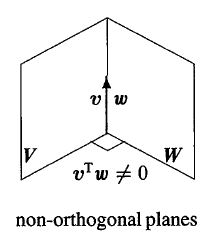
\includegraphics{week5/orthogonality}
\caption{Orthogonality is impossible when $\dim\bm U+\dim\bm V>\dim(\bm U\cup\bm V)$}
\end{figure}
\end{example}
\begin{remark}
When a vector is in two orthogonal subspaces, it \textit{must} be zero. It is \emph{perpendicular} to
itself. 
\\The reason is clear: this vector $\bm u\in\bm U$ and $\bm u\in\bm V$, so $\inp{\bm u}{\bm u}=0$. It has to be zero vector.
\end{remark}
If two subspaces are perpendicular, their basis must be ind.
\begin{theorem}
Assume $\{u_1,\dots,u_k\}$ is the basis for $\bm U$, $\{v_1,\dots,v_l\}$ is the basis for $\bm V.$ If $\bm U\perp\bm V$ ($u_i\perp v_j$ for $\forall i,j$), then $u_1,u_2,\dots,u_k,v_1,v_2,\dots,v_l$ must be ind.
\end{theorem}
\begin{proof}
Suppose there exists $\{\alpha_1,\dots,\alpha_k\}$ and $\{\beta_1,\dots,\beta_l\}$ such that
\[
\alpha_1u_1+\dots+\alpha_ku_k+\beta_1v_1+\dots+\beta_lv_l=\bm 0
\]
then equivalently,
\[
\alpha_1u_1+\dots+\alpha_ku_k=-(\beta_1v_1+\dots+\beta_lv_l).
\]
Then we set $\bm w=\alpha_1u_1+\dots+\alpha_ku_k$, obviously, $\bm w\in\bm U$ and $\bm w\in\bm V$.

 Hence it must be zero (This is due to remark above). Thus we have
\begin{gather*}
\alpha_1u_1+\dots+\alpha_ku_k=\bm 0\\
\beta_1v_1+\dots+\beta_lv_l=\bm 0.
\end{gather*}
Due to the independence, we have $\alpha_i=0$ and $\beta_j=0$ for $\forall i,j$. 
\end{proof}
\begin{corollary}
For subspaces $\bm U$ and $\bm V$, we obtain
\[
\dim(\bm U\cup\bm V)\le \dim(\bm U) + \dim(\bm V).
\]
\end{corollary}
For subspaces $\bm U$ and $\bm V\in\mathbb{R}^{n}$, if $\mathbb{R}^{n}=\bm U\cup\bm V$, and moreover, $n=\dim(\bm U)+\dim(\bm V)$, then we say $\bm V$ is the \emph{orthogonal complement} of $\bm U$.
\begin{definition}[orthogonal complement]
For subspaces $\bm U$ and $\bm V\in\mathbb{R}^{n}$, if $\dim(\bm U)+\dim(\bm V)=n$ and $\bm U\perp\bm V$, then we say $\bm V$ is the \emph{orthogonal complement} of $\bm U$. We denote $\bm V$ as $\bm U^{\perp}$.

Moreover, $\bm V=\bm U^{\perp}$ iff $\bm V^{\perp}=\bm U$.
\end{definition}
\begin{example}
Suppose $\bm U\cup\bm V=\mathbb{R}^{3}$, $\bm U=\Span\{\bm e_1,\bm e_2\}$. If $\bm V$ is the orthogonal complement of $\bm U$, then $\bm V=\Span\{\bm e_3\}$.
\end{example}

Next we study the relationship between the null space and the row space in $\mathbb{R}^n$.
\begin{theorem}[Fundamental theorem for linear alegbra, part 2] Given $\bm A\in\mathbb{R}^{m\times n}$,

\emph{$N(\bm A)$ is the orthogonal complement of the row space of $\bm A$, $\mathcal{C}(\bm A\trans)$ (in $\mathbb{R}^{n}$).}

\emph{$N(\bm A\trans)$ is the orthogonal complement of the column space $\mathcal{C}(\bm A)$ (in $\mathbb{R}^{m}$).}
\end{theorem}
\begin{proof}
\begin{itemize}
\item
Firstly, we show $\dim(N(\bm A))+\dim(\mathcal{C}(\bm A\trans))=n$:

We know that $\dim(N(\bm A))=n-r$ and $\dim(\mathcal{C}(\bm A\trans)) = r$, where $r=\rank(\bm A)$.

Hence $\dim(N(\bm A))+\dim(\mathcal{C}(\bm A\trans))=n$.
\item
Then we show $N(\bm A)\perp \mathcal{C}(\bm A\trans)$:

For any $x\in N(\bm A)$, if we set $\bm A=\begin{bmatrix}
a_1\trans\\a_2\trans\\\vdots\\a_m\trans
\end{bmatrix}$, then we obtain:
\[
\bm{Ax}=\begin{bmatrix}
a_1\trans\\a_2\trans\\\vdots\\a_m\trans
\end{bmatrix}\begin{bmatrix}
\bm x
\end{bmatrix}=\begin{bmatrix}
0\\0\\\vdots\\0
\end{bmatrix}
\]
Hence \textit{every row has a zero product with} $\bm x$, i.e., $\inp{a_i}{\bm x}=0$ for $\forall i\in\{1,2,\dots,m\}$.

For any $y=\sum_{i=1}^m\alpha_ia_i\in \mathcal{C}	(\bm A\trans)$, we obtain:
\[
\begin{aligned}
\inp{\bm x}{y}&=\inp{y}{\bm x}=\inp{\sum_{i=1}^m\alpha_ia_i}{\bm x}\\
&=\sum_{i=1}^{m}\alpha_i\inp{a_i}{\bm x}=0.
\end{aligned}
\]
Hence $\bm x\perp y$ for $\forall \bm x\in N(\bm A)$ and $y\in \mathcal{C}(\bm A\trans)$.\\
\end{itemize}
Hence $N(\bm A)^{\perp}=\mathcal{C}(\bm A\trans)$. Similarly, we have $N(\bm A\trans)^{\perp}=\mathcal{C}(\bm A)$. 
\end{proof}

\begin{corollary}
$\bm{Ax}=\bm b$ is solvable if and only if $\bm y\trans\bm A=\bm 0$ implies $\bm y\trans\bm b$=0.
\end{corollary}
\begin{proof} The following statements are equivalent:
\begin{itemize}
\item
$\bm{Ax}=\bm b$ is solvable.
\item
$\bm b\in \mathcal{C}(\bm A)$.
\item
$\bm b\in N(\bm A\trans)^{\perp}$
\item
$\bm y\trans\bm b=0$ for $\forall y\in N(\bm A\trans)$
\item
Given $\bm y\trans\bm A=\bm 0$, i.e., $y\in N(\bm A\trans)$, it implies $\bm y\trans\bm b=0$.
\end{itemize}
\end{proof}
The \emph{Inverse Negative Proposition} is more commonly useful:
\begin{corollary}
$\bm{Ax}=\bm b$ has no solution if and  and only if $\exists \bm y$ s.t. $\bm y\trans\bm A=0$ and $\bm y\trans\bm b\ne 0$.
\end{corollary}
We could extend this corollary into general case:
\begin{remark}
\begin{theorem}\label{theorem_12.3}
$\bm{Ax}\ge\bm b$ has no solution if and only if $\exists \bm y\ge\bm 0$ such that $\bm y\trans\bm A=\bm 0$ and $\bm y\trans\bm b\ge \bm 0$.
\end{theorem}
$\bm y\trans\bm A=0$ requires that there exists one linear combination of the row space to be zero.

The complete proof for this theorem is not required in this course. We only show the necessity case.
\begin{proof}[Necessity case.]
Suppose $\exists \bm y\ge\bm 0$ such that $\bm y\trans\bm A=\bm 0$ and $\bm y\trans\bm b\ge \bm 0$. Assume there exists $x^{*}$ such that $\bm Ax^{*}\ge\bm b$. By postmultiplying $\bm y\trans$ we have 
\[\bm y\trans\bm Ax^{*}\ge\bm y\trans\bm b>\bm 0
\implies 
\bm 0>\bm 0.
\]
which is a contradiction!
\end{proof}
\end{remark}

\begin{example}
Given the system 
\begin{align}
x_1+x_2&\ge1\label{Eq:6:3}
\\
-x_1&\ge-1\label{Eq:6:4}
\\
-x_2&\ge2\label{Eq:6:5}
\end{align}
Eq.(\ref{Eq:6:3})$\x$1+Eq(\ref{Eq:6:4})$\x$1+Eq.(\ref{Eq:6:5})$\x$1 gives
\[
0\ge 2
\]
which is a contradiction!\\
So the key idea of theorem (\ref{theorem_12.3}) is to construct a linear combination of row space to let it become zero. If the right hand is larger than zero, then this system has no solution.
\end{example}
\begin{remark}
\begin{corollary}
If $\bm A=\bm A\trans$, then $N(\bm A\trans)^{\perp}=\mathcal{C}(A)=\mathcal{C}(\bm A\trans)=N(\bm A)$.
\end{corollary}
\begin{corollary}\label{corollary_12.5}
The system $\bm{Ax}=\bm b$ may not have a solution, but $\bm A\trans\bm A\bm x=\bm A\trans\bm b$ always have at least one solution for $\forall\bm b$.
\end{corollary}
\begin{proof}
Since $\bm A\trans\bm A$ is symmetric, we have $\mathcal{C}(\bm A\trans\bm A)=\mathcal{C}(\bm A\bm A\trans)$. Show by yourself that $\mathcal{C}(\bm A\bm A\trans)=\mathcal{C}(\bm A\trans)$, hence $\mathcal{C}(\bm A\trans\bm A)=\mathcal{C}(\bm A\trans)$.

For any vector $\bm b$, we have $\bm A\trans\bm b\in \mathcal{C}(\bm A\trans)\implies\bm A\trans\bm b\in \mathcal{C}(\bm A\trans\bm A)$, which means there exists a linear combination of the columns of $\bm A\trans\bm A$ that equals to $\bm b$.

Or equivalently, there exists a solution to $\bm A\trans\bm A\bm x=\bm A\trans\bm b$.
\end{proof}
\begin{corollary}\label{corollary_12.6}
$\bm A\trans\bm A$ is invertible if and only if $\bm A$ is full column rank, i.e., columns of $\bm A$ are ind.
\end{corollary}
\begin{proof}
We have shown that $C(\bm A\trans\bm A)=C(\bm A\trans)$.

Hence $C(\bm A\trans\bm A)^{\perp}=C(\bm A\trans)^{\perp}\implies N(\bm A\trans\bm A)=N(\bm A)$.

Thus, the following statements are equivalent:
\begin{itemize}
\item
$\bm A$ has ind. columns
\item
$N(\bm A)=\{\bm 0\}$
\item
$N(\bm A\trans\bm A)=\{\bm 0\}$
\item
$\bm A\trans\bm A$ is invertible.
\end{itemize}
\end{proof}
\end{remark}
\subsection{Least Squares Approximations}
The linear system $\bm{Ax}=\bm b$ often has no solution, if so, what should we do?

We cannot always get the error $\bm e=\bm b-\bm{Ax}$ down to zero, so we want to use \textit{least square method} to minimize the error. In other words, our goal is to
\[
\min_{\bm x\in\mathbb{R}^n}\bm e^2:=\min_{\bm x}\|\bm{Ax}-\bm b\|^2=\sum_{i=1}^{m}(a_i\trans\bm x-b_i)^2
\]
where $\bm A\in\mathbb{R}^{m\times n}$ and $\bm b\in\mathbb{R}^m$. The minimizer $\bm x$ is called the \emph{linear least squares solution}.

\subsubsection{Least Squares by Convex Optimization}
Firstly, you should know some basic calculus knowledge for matrix:
\paragraph{The Chian Rule} Given two vectors $f(x),g(x)$ of appropriate size,
\[
\frac{\partial(f\trans g)}{\partial x}=\frac{\partial f(x)}{\partial x}g(x)+\frac{\partial g(x)}{\partial x}f(x)
\]
\paragraph{Examples of Matrix Derivative}
\begin{align}
\frac{\partial(a\trans \bm x)}{\partial \bm x}&=a\\
\frac{\partial(a\trans \bm A\bm x)}{\partial \bm x}&=\frac{\partial((\bm A\trans a)\trans\bm x)}{\partial \bm x}=\bm A\trans a\\
\frac{\partial(\bm A\bm x)}{\partial \bm x}&=\bm A\trans\\
\frac{\partial(\bm x\trans\bm A\bm x)}{\partial \bm x}&=\bm A\bm x+\bm A\trans\bm x
\end{align}

Thus, in order to minimize $\|\bm{Ax}-\bm b\|^2=(\bm{Ax}-\bm b)\trans(\bm{Ax}-\bm b)$, it suffices to let its \emph{derivative} with respect to $\bm x$ to be \emph{zero.} (Since $\|\bm{Ax}-\bm b\|^2$ is convex, which will be discussed in detail in other courses.) Hence we have:
\[\begin{aligned}
\frac{\partial (\bm{Ax}-\bm b)\trans(\bm{Ax}-\bm b)}{\partial \bm x}&=\frac{\partial(\bm{Ax}-\bm b)}{\partial \bm x}(\bm{Ax}-\bm b)+\frac{\partial(\bm{Ax}-\bm b)}{\partial \bm x}(\bm{Ax}-\bm b)\\
&=2\frac{\partial(\bm{Ax}-\bm b)}{\partial \bm x}(\bm{Ax}-\bm b)\\
&=2(\frac{\partial(\bm A\bm x)}{\partial \bm x}-\frac{\partial(\bm b)}{\partial \bm x})(\bm{Ax}-\bm b)\\
&=2\bm A\trans(\bm{Ax}-\bm b)=\bm 0.
\end{aligned}
\]
Or equivalently, 
\[
\bm A\trans\bm{Ax}=\bm A\trans\bm b.
\]
According to corollary (\ref{corollary_12.5}), this equation always exists a solution. This equation is called the \emph{normal equation}.
\begin{theorem}\label{theorem_12.4}
A vector $\bm x_{\text{LS}}$ is an optimal solution to the least squares problem
\begin{subequations}
\begin{equation}
\min_{\bm x\in\mathbb{R}^n}\|\bm b-\bm{Ax}\|_2^2
\end{equation}
if and only if it satisfies
\begin{equation}
\bm A\trans\bm A\bm x_{\text{LS}} = \bm A\trans\bm b.
\end{equation}
\end{subequations}
\end{theorem}
\subsubsection{Fit a stright line}
Given a collection of data $(\bm x_i,y_i)$ for $i=1,\dots,m$, we can use a stright line to fit these points:
\[
\left\{
\begin{aligned}
y_1&=a_0+a_1x_{1,1}+a_2x_{1,2}+\dots+a_nx_{1,n}+\varepsilon_1\\
y_2&=a_0+a_1x_{2,1}+a_2x_{2,2}+\dots+a_nx_{2,n}+\varepsilon_2\\
\vdots\\
y_m&=a_0+a_1x_{m,1}+a_2x_{m,2}+\dots+a_nx_{m,n}+\varepsilon_m
\end{aligned}
\right.
\]
Our fit line is 
\[
\hat y=a_0+a_1x_1+a_2x_2+\dots+a_nx_n
\]
In \textit{compact matrix form}, we have
\[
\begin{bmatrix}
y_1\\y_2\\\vdots\\y_n
\end{bmatrix}
=\begin{bmatrix}
1&x_{1,1}&x_{1,2}&\dots&x_{1,n}\\
1&x_{2,1}&x_{2,2}&\dots&x_{2,n}\\
\vdots&\vdots&&&\\
1&x_{m,1}&x_{m,2}&\dots&x_{m,n}\\
\end{bmatrix}\begin{bmatrix}
a_0\\a_1\\a_2\\\vdots\\a_{n}
\end{bmatrix}+\begin{bmatrix}
\varepsilon_1\\\varepsilon_2\\\vdots\\\varepsilon_m
\end{bmatrix}
\]
Or equivalently, we have 
\[
\bm y=\bm{Ax}+\bm \varepsilon
\]
where $\bm A =\begin{bmatrix}
1&x_{1,1}&x_{1,2}&\dots&x_{1,n}\\
1&x_{2,1}&x_{2,2}&\dots&x_{2,n}\\
\vdots&\vdots&&&\\
1&x_{m,1}&x_{m,2}&\dots&x_{m,n}\\
\end{bmatrix}_{m\times (n+1)}$, $\bm x=\begin{bmatrix}
a_0\\a_1\\a_2\\\vdots\\a_{n}
\end{bmatrix}_{(n+1)\times 1}$, $\bm \varepsilon=\begin{bmatrix}
\varepsilon_1\\\varepsilon_2\\\vdots\\\varepsilon_m
\end{bmatrix}_{m\times 1}$.\\
Our goal is to minimize $\|\hat{\bm y}-\bm y\|^2=\|\bm{Ax}-\bm y\|^2$. Then by theorem (\ref{theorem_12.4}), it suffices to sovle $\bm A\trans\bm A\bm x=\bm A\trans\bm y$.

\subsection{Projections}
In corollary (\ref{corollary_12.6}), we know that if $\bm A$ has ind. columns, then $\bm A\trans\bm A$ is invertible. On this condition, the normal equation $\bm A\trans\bm A\bm x=\bm A\trans\bm b$ has the unique solution $\bm x^{*}=(\bm A\trans\bm A)^{-1}\bm A\trans\bm b$, which follows that the error $\bm b-\bm A\bm x^{*}$ is minimized. Note that $\bm A\bm x^{*}=\bm A(\bm A\trans\bm A)^{-1}\bm A\trans\bm b$ is \emph{approximately} equal to $\bm b$. 
\begin{itemize}
\item
If $\bm b$ and $\bm{A}\bm x^{*}$ are exactly in the same space, i.e., $\bm b\in\mathcal{C}(\bm A)$, then $\bm{A}\bm x^{*}=\bm b$. The error is equal to zero.
\item
Otherwise, just as the Figure (\ref{figure_12.2}) shown, $\bm A\bm x^{*}$ is the projection of $\bm b$ to subspace $\mathcal{C}(\bm A)$.
\end{itemize}
\begin{figure}[t]
\centering
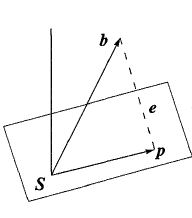
\includegraphics{week5/projection}
\caption{The projection of $\bm b$ onto a subspace $\bm S:=\mathcal{C}(\bm A)$.}\label{figure_12.2}
\end{figure}
\begin{definition}[Projection]
Let $\bm S\in\mathbb{R}^{m}$ be a non-empty closed set and $\bm b\in\mathbb{R}^m$ be given. Then the projection of $\bm b$ onto the set $\bm S$ is the solution to
\[
\min_{\bm z\in\bm S}\|\bm z-\bm b\|_2^2,
\]
where we use notation $\Proj_{\bm S}(\bm b)$ to denote the projection of $\bm b$ onto $\bm S$.
\end{definition}
By definition, the projection of $\bm b$ onto the subspace $\mathcal{C}(\bm A)$ is given by 
\[
\Proj_{\mathcal{C}(\bm A)}(\bm b):=\bm A\bm x^*,\quad
\text{where }\bm x^*=\arg\min_{\bm x\in\mathbb{R}^n}\|\bm{Ax} - \bm b\|.
\]

\begin{definition}[Projection matrix]
Given the projection
\[
\Proj_{C(\bm A)}(\bm b):=\bm A\bm x^{*}=\bm A(\bm A\trans\bm A)^{-1}\bm A\trans\bm b,
\]
since $[\bm A(\bm A\trans\bm A)^{-1}\bm A\trans]\bm b$,
we call the projection operator $\bm P:=\bm A(\bm A\trans\bm A)^{-1}\bm A\trans$ as the \emph{projection matrix} of $\bm A$.
\end{definition}
\begin{definition}[Idempotent]
Let $\bm A$ be a \emph{square} matrix that satisfies $\bm A=\bm A\bm A$, then $\bm A$ is called an \emph{idempotent} matrix.
\end{definition}
Let's show that the projection matrix is \textit{idempotent}:
\[
\begin{aligned}
\bm P^{2}&=\bm A(\bm A\trans\bm A)^{-1}\bm A\trans\bm A(\bm A\trans\bm A)^{-1}\bm A\trans\\
&=\bm A(\bm A\trans\bm A)^{-1}(\bm A\trans\bm A)(\bm A\trans\bm A)^{-1}\bm A\trans\\
&=\bm A(\bm A\trans\bm A)^{-1}\bm A\trans=\bm P.
\end{aligned}
\]

\subsubsection{Observations}
\begin{itemize}
\item
Suppose $\bm b\in \mathcal{C}(\bm A)$, i.e., $\exists \bm x$ s.t. $\bm{Ax}=\bm b$. Then the projection of $\bm b$ is exactly $\bm b$:
\[
\begin{aligned}
\bm{Pb}&=\bm A(\bm A\trans\bm A)^{-1}\bm A\trans(\bm b)\\
&=\bm A(\bm A\trans\bm A)^{-1}\bm A\trans(\bm{Ax})\\
&=\bm A(\bm A\trans\bm A)^{-1}(\bm A\trans\bm A)\bm x\\
&=\bm{Ax}=\bm b.
\end{aligned}
\]
\item
Assume $\bm A$ has only one column, say, $\bm a$. Then we have
\[\begin{aligned}
\bm x^{*}&=(\bm A\trans\bm A)^{-1}\bm A\trans\bm b=\frac{\bm a\trans\bm b}{\bm a\trans\bm a}\\
\bm A\bm x^{*}&=\bm{Pb}=\bm A(\bm A\trans\bm A)^{-1}\bm A\trans(\bm b)=\frac{\bm a\trans\bm b}{\bm a\trans\bm a}\times\bm a=\frac{\bm a\trans\bm b}{\|\bm a\|^2}\times\bm a
\end{aligned}
\]
More interestingly, 
\[\frac{\bm a\trans\bm b}{\|\bm a\|^2}\times\bm a=\frac{\|\bm a\|\|\bm b\|\cos\theta}{\|\bm a\|^2}\times\bm a=\|\bm b\|\cos\theta\times\frac{\bm a}{\|\bm a\|}\]
which is the projection of $\bm b$ onto a line $\Span\{\bm a\}$. (Shown in figure (\ref{Fig:6:3}).)
\begin{figure}[H]
\centering
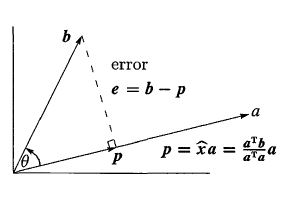
\includegraphics[width=10cm]{week5/projection_line}
\caption{The projection of $\bm b$ onto a line $\bm a$.}
\label{Fig:6:3}
\end{figure}
More generally, we can write the projection of $\bm b$ onto the line $\Span\{\bm a\}$ as:
\[
\Proj_{\Span\{\bm a\}}(\bm b)=\frac{\inp{\bm a}{\bm b}}{\inp{\bm a}{\bm a}}\bm a
\]
\paragraph{Changing an Orthogonal Basis}
Note that the error $\bm b-\Proj_{\Span\{\bm a\}}(\bm b)$ is perpendicular to $\bm a$, and $\bm b-\Proj_{\Span\{\bm a\}}(\bm b)\in\Span\{\bm a,\bm b\}.$

If we define $\bm b'=\bm b-\Proj_{\Span\{\bm a\}}(\bm b)$, then it's easy to check that $\Span\{\bm a,\bm b'\}=\Span\{\bm a,\bm b\}$ and $\bm a\perp\bm b'$. 

Hence, we convert the basis $\{\bm a,\bm b\}$ into another basis $\{\bm a,\bm b'\}$ such that the elements are orthogonal to each other. For general subspace we could also use this approach to obtain an orthogonal basis, which will be discussed in next lecture. 
\end{itemize}









%\section{Friday}\index{week7_Thursday_lecture}

\subsection{Polynomials}
\begin{definition}[polynomial]
Let $k$ be a field, and $f=\sum_{i=0}^nc_ix^i$ be a polynomial in $k[x]$. An element $a\in k$ is a root of $f$ if
\[
f(a)=\sum_{i=0}^nc_ia^i=0
\]
in $k$.
\end{definition}
question: what is $k[x]$?
\begin{corollary}
For all $f\in k[x]$, $a\in k$, then there exists $q\in k[x]$ such that
\[
f=q(x-a)+f(a)
\]
\end{corollary}
\begin{proof}
By division theorem, there exists $q,r\in k[x]$ such that
\[
f=q\cdot (x-a)+r,\quad
\mbox{deg}r<\mbox{deg}(x-a)=1
\]
which implies $r$ is a constant. Evaluate both sides for $x=a$, we have
\[
f(a)=r.
\]
\end{proof}
\begin{proposition}[root theorem]
Let $k$ be a field, $f$ a polynomial is $k[x]$. Then $a\in k$ is a root of $f$ iff $(x-a)$ divides $f$ in $k[x]$.
\end{proposition}
\begin{proof}
For forward direction, there exists $q\in k[x]$ such that
\[
f=q(x-a)+f(a)=q(x-a)\implies (x-a)|f
\]
For the reverse direction, if $f=q(x-a)$ for some $q\in k[x]$, then $f(a)=q(a)(a-a)=0$, i.e., $a$ is a root of $f$.
\end{proof}
\begin{theorem}
Let $k$ be a field, $f$ a nonzero polynomial in $k[x]$
\begin{enumerate}
\item
If $f$ has some degree $n$, then it has at most $n$ roots in $k$
\item
If $f$ has degree $n$ and $a_1,\dots,a_n\in k$ are distinct roots of $f$, then
\[
f=c\prod_{i=1}^n(x-a_i)
\]
for some $c\in k$.
\end{enumerate}
\end{theorem}
\begin{proof}
\begin{enumerate}
\item
We show the first part by induction. Suppose it holds for all nonzero polynomails with degree strictly less than $n$, and $\mbox{deg}f=n$. If $f$ has no roots in $k$, the proof is complete, otherwise suppose a root $a\in k$. There exists $q\in k[x]$ such that
\[
f=q(x-a)
\]
For the any other root $b\in k$, we have 
\[
0=q(b)(b-a)
\]
Since $k$ is a firld, it has no zero divisors, which implies $q(b)=0$, since $b-a\ne0$. Thus $b$ is a root of $q$. Since $\mbox{deg}q<n$, by induction we imply $q$ has at most $n-1$ roots, i.e., $f$ has at most $n-1$ roots that are different from $a$.
\item
If $n=1$, then $f=c_0+c_1x$ for some $c_i\in k$ with $c_1\ne0$, which implies
\[
0=f(a_1)=c_0+c_1a_1\implies c_0=-c_1a_1\implies
f=-c_1a_1+c_1x=c_1(x-a_1)
\]
Suppose $n>1$, and the claim holds for all $n'\in\mathbb{N}$ such that $n'<n$. By previuos claim, there exists $q\in k[x]$ such that
\[
f=q(x-a_n)
\]
Since $\mbox{deg}q=n-1$, and for $1\le i<n$, we have
\[
0=f(a_i)=q(a_i)(a_i-a_n)\implies q(a_i=0),
\]
which implies $a_1,\dots,a_{n-1}$ are $n-1$ distinct roots of $q$ as well. Thus there exists $c\in k$ s.t.
\[
q=c(x-a_1)\cdots(x-a_{n-1}),
\]
which follows that
\[
f=q(x-a_n)=c(x-a_1)\cdots(x-a_n)
\]
\end{enumerate}
\end{proof}

\begin{corollary}
Let $k$ be a field. Let $f,g$ be nonzero polynomails in $k[x]$. Let $n=\max\{\mbox{deg}f,\mbox{deg}g\}$. If $f(a)=g(a)$ for $n+1$ distinct $a\in k$, then $f=g$.
\end{corollary}
\begin{proof}
Let $h=f-g$, then $\mbox{deg}h\le n$. There are $n+1$ distinct elements $a\in k$ s.t. $h(a)=0$. If $h\ne0$, then it is a nonzero polynomial of degree $\le n$ which has $n+1$ distinct roots, which is a constraction. $h=0$ implies $f=g$.
\end{proof}
\begin{definition}
A polynomail in $k[x]$ is called a \emph{monic polynomial} if its leading coefficient is $1$.
\end{definition}
\begin{theorem}
Let $k$ be a field, then the ring $k[x]$ is a PID.
\end{theorem}
\begin{corollary}
Let $k$ be a field, and $f,g$ be nonzero polynomials in $k[x]$. There exists a unique monic polynomial $d\in k[x]$ with the following properties:
\begin{enumerate}
\item
$(f,g)=(d)$
\item
$d$ divides both $f$ and $g$, i.e., there exists $a,b\in k[x]$ s.t. $f=ad,g=bd$
\item
There are polynomials $p,q\in k[x]$ such that $d=pf+qg$
\item
If $h\in k[x]$ is a divisor of $f,g$, then $h$ divides $d$.	
\end{enumerate}
This $d\in k[x]$ is called the \emph{greatest common divisor} (GCD) of $f$ and $g$. We say $f$ and $g$ are \emph{relatively prime} if their GCD is 1.
\end{corollary}
\begin{proof}
By the PID theorem, there exists $d=\sum_{n=0}^\infty a_ix^i\in k[x]$ such that $(d)=(f,g)$. Replacing $d$ with $a_n^{-1}d$, we assume $d$ is a monic polynomial. It remains to show that $d$ is unique. 

Suppose $(d)=(d')$, there exists nonzero $p,q\in k[x]$ such that
\[
d'=pd,\quad
d=qd'
\]
which follows that
\[
\mbox{deg}d'=\mbox{deg}d+\mbox{deg}p,\quad
\mbox{deg}d=\mbox{deg}q+\mbox{deg}d'=\mbox{deg}q+\mbox{deg}d+\mbox{deg}p,
\]
i.e., $\mbox{deg}p=\mbox{deg}q=0$. Thus $\mbox{deg}d=\mbox{deg}d'$. Comparing the leading coefficients of $d'$ and $pd$, we have $p=1$, i.e., $d=d'$.

The remaining part follows similarly.
\end{proof}
\begin{definition}[Irreducible]
Let $R$ be a commutative ring. A non-zero element $p\in R$ which is not a unit is said to be \emph{irreducible} if $p=ab$ implies that either $a$ or $b$ is a unit.
\end{definition}
\begin{example}
The set of irreducible elements in the ring $\mathbb{Z}$ is
\[
\{\pm p\mid p\mbox{ is a prime number}\}
\]
\end{example}
Let $k$ be a field.
\begin{proposition}
A polynomial $f\in k[x]$ is a unit iff it is a \emph{nonzero} constant polynomial.
\end{proposition}
\begin{proposition}
A nonzero nonconstant polynoimial $p\in k[x]$ is \emph{irreducible} iff there is no $f,g\in k[x]$ with $\mbox{deg}f,\mbox{deg}g<\mbox{deg}p$, such that $fg=p$.
\end{proposition}
\begin{proof}
\begin{enumerate}
\item
Suppose $p$ is irreducible, and $p=fg$ for some $f,g\in k[x]$ such that $\mbox{deg}f,\mbox{deg}g<\mbox{deg}p$. Then $p=fg$ implies that $\mbox{deg}f,\mbox{deg}g$ are both positive. By previous lemma, both $f,g$ are non-units, which is a contradiction.
\item
Conversely, suppose $p$ is a nonzero non-unit in $k[x]$, which is not equal to $fg$ for $\forall f,g\in k[x]$ with $\mbox{deg}f,\mbox{deg}g<\mbox{deg}p$. Then $p=ab$ for $a,b\in k[x]$ implies that either $a$ or $b$ must have the same degree as $p$, and the otehr factor must be a nonzero constant, i.e., a unit in $k[x]$. Thus $p$ is irreducible.
\end{enumerate}
\end{proof}

\begin{proposition}[Euclid's Lemma]
Let $k$ be a field. Let $f,g$ be polynomials in $k[x]$. Let $p$ be an irreducible polynomial in $k[x]$. If $p|fg$ in $k[x]$, then $p|f$ or $p|g$.
\end{proposition}
\begin{proof}
Suppose $p$ not divides $f$, then any \emph{common divisor} of $p$ and $f$ must have degree strictly less than $\mbox{deg}p$. Since $p$ is irreducible, this implies that any common divisor of $p$ and $f$ is a nonzero constant. Thus the GCD of $p$ and $f$ is 1. There exists $a,b\in k[x]$ such that
\[
ap+bf=1\implies
apg+bfg=g
\]
Since $p$ divides the LHS, it also divides the RHS.
\end{proof}
\begin{proposition}
If $f,g\in k[x]$ are relatively prime, and both divide $h\in k[x]$, then $fg|h$.
\end{proposition}
question
\begin{theorem}[Unique Factorization]
Let $k$ be a field. Every non-constant polynomial $f\in k[x]$ may be written as
\[
f=cp_1\cdots p_n
\]
where $c$ is a non-zero constant, and each $p_i$ is a monic irreducible polynomials in $k[x]$. The factorization is \emph{unique} up to the ordering of the factors.
\end{theorem}
\begin{proof}
Similar to the proof of unique factorization for $\mathbb{Z}$
\end{proof}
\begin{theorem}
Let $k$ be a field, $p$ be a polynomial in $k[x]$. The following statements are equivalent:
\begin{enumerate}
\item
$k[x]/(p)$ is a field
\item
$k[x]/(p)$ is an integral domain
\item
$p$ is irreducible in $k[x]$.
\end{enumerate}
\end{theorem}
\begin{proof}
\begin{enumerate}
\item
(2) implies (3): If $p$ is not irreducible, then there exists $f,g\in k[x]$ with degree strictly less than that of $p$, such that $p=fg$.

It's clear that $p$ does not divide $f$ or $g$ in $k[x]$. The equivalence classes $\bar f$ and $\bar g$ of $f$ and $g$, respectively, modulo $(p)$ is not equal to zero in $k[x]/(p)$. (question) On the other hand, $\bar f\cdot\bar g=\bar{fg}=\bar p=0$ in $k[x]/(p)$, which implies that $k[x]/(p)$ is not an integral domain, which is a contradction.
\item
(3) implies (1): By definiton, the multiplicative identity $1$ of a field is different from addictive identity $0$. We first check that the equivalence lcass $1\in k[x]$ in $k[x]/(p)$ is not zero. Since $p$ is irreducible, we have $\mbox{deg}p>0$, and $1\notin(p)$. Therefore $1+(p)\ne 0+(p)$ in $k[x]/(p)$.

Next, we need to show the existence of multiplicative inverse of any nonzero element in $k[x]/(p)$. Given any $f\in k[x]$ whose equivalence $\bar f$ modulo $(p)$ is nonzero in $k[x]/(p)$, we want to constracut $\bar{f}^{-1}$. Since $\bar{f}\ne0$ in $k[x]/(p)$, we have $f-0\notin(p)$, i.e., $p$ does not divide $f$. Since $p$ is irreducible, we have $gcd(p,f)=1$. There exists $g,h\in k[x]$ such that $fg+hp=1$. Thus $\bar{f}^{-1}=\bar{g}$. This is becasue $fg-1=hp$ implies $fg-1\in(p)$, i.e., $\bar{f}\bar{g}=\bar{fg}=1$ in $k[x]/(p)$.


\end{enumerate}
\end{proof}
\subsection{Polynomials over $\mathbb{Z}$ and $\mathbb{Q}$}
\begin{theorem}
Let $f=a_0+a_1x+\cdots+a_nx^n$ be a polynomial in $\mathbb{Q}[x]$, with $a_i\in\mathbb{Z}$. Every rational root $r$ of $f$ in $\mathbb{Q}$ has the form $r=b/c$ $(b,c\in\mathbb{Z})$, where $b|a_0$ and $c|a_n$
\end{theorem}
\begin{proof}
Let $r=b/c$ be a rational root of $f$, where $b,c$ are relatively prime integers. We have
\[
0=\sum_{i=1}^na_i(b/c)^i
\]
Multiplying both sides above equation by $c^n$, we have
\[
0=a_0c^n+a_1c^{n-1}b+\cdots+a_nb^n
\]
or equivalently,
\[
a_0c^n=-(a_1c^{n-1}+\cdots+a_nb^n)
\]
Since $b$ divides the RHS, and $b,c$ are relatively prime, $b$ must divide $a_0$. Similarly,
\[
a_nb^n=-(a_0c^n+\cdots+a_{n-1}cb^{n-1})
\]
It is clear that $c$ divides $a_n$.
\end{proof}
\begin{definition}
A polynomial $f\in\mathbb{Z}[x]$ is said to be \emph{primitive} if the gcd of its coefficients is 1.
\end{definition}
\begin{remark}
Note that if $f$ is monic, i.e., its leading coefficient is 1, then it is primitive. If $d$ is the gcd of the coefficients of $f$, then $\frac{1}{d}f$ is a primitive polynomial in $\mathbb{Z}[x]$.
\end{remark}
\begin{theorem}[Gauss's Lemma]
If $f,g$ are both primitive, then $fg$ is primitive.
\end{theorem}
\begin{proof}
Write $f=\sum_{k=0}^ma_kx^k$ and $g=\sum_{k=0}^nb_kx^k$, then $fg=\sum_{k=0}^{m+n}c_kx^k$, where
\[
c_{k}=\sum_{i+j=k}a_ib_j.
\]
Assume that $fg$ is not primitive, then there exists a prime $p$ such that $p$ divides $c_k$ for $k=0,1,\dots,m+n$. Since $f$ is primitive, there exists smallest $u$ s.t. $a_u$ is not dividible by $p$; similarly, a smallest $v$ s.t. $b_v$ is not divisible by $p$. We have
\[
c_{u+v}=\left(\sum_{i+j=u+v,(i,j)\ne(u,v)}a_ib_j\right)+a_ub_v,
\]
which implies that
\[
a_ub_v=c_{u+v}-
\left(\sum_{i+j=u+v,i<u}a_ib_j\right)
-
\left(\sum_{i+j=u+v,i>u}a_ib_j\right)
\]
By the minimum conditons on $u$ and $v$, each term on the RHS of the above equation is divisible by $p$. Thus $p$ divides $a_u$ and $b_v$, which implies that $p$ divides either $a_u$ or $b_v$, which is a contradiction.
\end{proof}
\begin{proposition}
Every nonzero $f\in\mathbb{Q}[x]$ has a unique factorization:
\[
f=c(f)f_0,
\]
where $c(f)$ is a positive rational number, and $f_0$ is a primitive polynomial in $\mathbb{Z}[x]$.
\end{proposition}
\begin{definition}
The rational number $c(f)$ is called the \emph{content} of $f$.
\end{definition}















%\section{Assignment Six}\index{Assignment_Six}
\begin{enumerate}
\item
Find the \textit{determinant} of the linear transformation $T(f(t))=f(3t-2)$ from $\mathbb{P}_2$ to $\mathbb{P}_2$.
\item
Suppose that $\bm A$ is a $m$ by $n$ real matrix. And suppose that $\bm{Ax}=\bm0$ and $\bm A\trans\bm y=2\bm y.$ Show that $\bm x$ is \textit{orthogonal} to $\bm y$.
\item
State and justify whether the following three statements are True or False (give an
example in either case):
\begin{enumerate}
\item
$\bm Q^{-1}$ is an \textit{orthogonal} matrix when $\bm Q$ is an \textit{orthogonal} matrix.
\item
If $\bm Q$ (a $m$ by $n$ matrix with $m>n$) has \textit{orthonormal columns}, then $\|\bm{Qx}\|=\|\bm x\|.$
\item
If $\bm Q$ (a $m$ by $n$ matrix with $m>n$) has \textit{orthonormal columns}, then $\|\bm{Q\trans\bm y}\|=\|\bm y\|.$
\end{enumerate}
\item
Let us make $P(\mathbb{R})$ into an \textit{inner product space} using the inner product
\[
\inp{p}{q}=\int_{-1}^{1}p(x)q(x)\diff x
\]
Recall that we say a function is \textit{even} if $\forall x$ we have $f(-x)=f(x)$ and \textit{odd} if $\forall x$ we have $f(-x)=-f(x).$\\
$W_1$ corresponds to the set of \textit{odd polynomials} and $W_2$ the set of \textit{even polynomials}. Show that $W_1=W_2^{\perp}.$
\item
Let $\bm V=\mathbb{R}^3,$ $\bm U$ the \textit{orthogonal complement} to $\Span\left\{\begin{pmatrix}
1\\2\\-5
\end{pmatrix}\right\}$. Find an \textit{orthonormal basis}
of $\bm U$.
\item
Find the best line $C+Dt$ to fit $b=4,2,-1,0,0$ at times $t=-2,-1,0,1,2$.
\end{enumerate}
%%
\chapter{Week4}

\section{Convergence}\index{week4_Friday_lecture}

\begin{definition}[Convergent]
An infinite sequence $\{z_n\}$ of complex numbers has a limit $z_0$, if for $\forall$ $\varepsilon>0$, there exists a positive integer $n_0$ such that
\[
\begin{array}{ll}
|z_n-z|<\varepsilon,
&
\mbox{whenever }n>n_0
\end{array}
\]
We say the sequence $z_n$ converges to $z$ and write as
\[
\lim_{n\to\infty}z_n=z
\]
When the sequence does not have a limit, then it diverges.
\end{definition}
The uniqueness of limit of a seuqnece is guaranteed.

\begin{proposition}
For $z_n=x_n+iy_n$, we have 
\[
\lim_{n\to\infty}z_n=x+iy
\]
if and only if
\[
\begin{array}{lll}
\lim_{n\to\infty}x_n=x,
&
\mbox{and}
&
\lim_{n\to\infty}y_n=y
\end{array}
\]
\end{proposition}

\begin{definition}[Convergent Series]
An infinite \emph{series} $\sum_{n=1}^\infty z_n$ of complex numbers converges to the sum $S$ if the partial sum sequences
\[
S_N=\sum_{n=1}^Nz_n
\]
converges to $S$, then we write
\[
\sum_{n=1}^\infty z_n=S.
\]
\end{definition}

\begin{proposition}
For $z_n=x_n+iy_n$, we have 
\[
\sum_{n=1}^\infty z_n=X+iY
\]
if and only if
\[
\begin{array}{lll}
\sum_{n=1}^\infty x_n=X
&
\mbox{and}
&
\sum_{n=1}^\infty y_n=Y
\end{array}
\]
\end{proposition}

\begin{proposition}
The series $\sum_{n=1}^\infty z_n$ converges implies that $\lim_{n\to\infty}z_n=0$.
\end{proposition}

\begin{definition}[Absolute Convergence]
The series $\sum_{n=1}^\infty z_n$ is said to be \emph{absolutely convergent} if
\[
\sum_{n=1}^\infty|z_n|
\]
converges, i.e., $\sum_{n=1}^\infty|x_n|$ and $\sum_{n=1}^\infty|y_n|$ converge.
\end{definition}
\begin{proposition}
Absolute convergence implies convergence
\end{proposition}

\begin{definition}[Remainder]
The \emph{remainder} $\rho_N$ of a series after $N$ terms is defined by:
\[
\rho_N=\sum_{n=N+1}^\infty S_n
\]
\end{definition}
\begin{proposition}
A series converges to a number $S$ iff the sequence of remainders tends to zero.
\end{proposition}

It's easy to verifty that
\[
\sum_{n=0}^\infty z_n=\frac{1}{1-z},\qquad\mbox{whenever }|z|<1
\]
with the aid of partial sums and remainders.

\subsection{Taylor Series}
\begin{definition}[Power Series]
The power series has the form
\[
\sum_{n=0}^\infty a_n(z-z_0)^n
\]
\end{definition}

\begin{theorem}[Convergent of Taylor Series]
Suppose $f$ is \emph{analytic} on $|z-z_0|<R$, then 
\begin{equation}
f(z)=\sum_{n=0}^\infty \frac{f^{(n)}(z_0)}{n!}(z-z_0)^n,
\end{equation}
for $|z-z_0|<R$, i.e., $f(z)$ admits its Taylor expansion at $z=z_0$ in this rigion.
\end{theorem}
\begin{remark}
Typically, when $z_0=0$, we say this series is the \emph{Maclaurin series}.
\end{remark}
\begin{proof}
\textbf{Step 1: Applying Cauchy Integral Formula.}
For fixed $z$, let $r:=|z-z_0|<R$ and take $r_0$ such that $r<r_0<R$. Construct a contour $C_0:\{z\in\mathbb{C}\mid |z-z_0|=r_0\}$ in the positive sense, which follows that
\begin{subequations}
\begin{align}
f(z)&=\frac{1}{2\pi i}\int_{C_0}\frac{f(s)}{s-z}\diff s\label{Eq:4:2:b}
\end{align}

\textbf{Step 2: Expand $1/(s-z)$.} With some calculation, we obtain
\begin{align}\label{Eq:4:2}
\frac{1}{s-z}&=\frac{1}{s-z_0}\cdot\frac{1}{1-\frac{z-z_0}{s-z_0}}\\
&=\frac{1}{s-z_0}\left\{1+\frac{z-z_0}{s-z_0}+\cdots+(\frac{z-z_0}{s-z_0})^{N-1}+\frac{(\frac{z-z_0}{s-z_0})^{N}}{1 - \frac{z-z_0}{s-z_0}}\right\}\label{Eq:4:2:d}\\
&=\frac{1}{s-z_0}+\frac{z-z_0}{(s-z_0)^2}+\cdots+\frac{(z-z_0)^{N-1}}{(s-z_0)^N}+\frac{(z-z_0)^N}{(s-z)(s-z_0)^N}\label{Eq:4:2:e}
\end{align}
where $(\ref{Eq:4:2:d})$ is because that
\[
\frac{1}{1-c}=1+c+c^2+\cdots+c^{N-1}+\frac{c^N}{1-c}. 
\]
Substituting (\ref{Eq:4:2:e}) into (\ref{Eq:4:2:b}), we obtain
\begin{align*}
f(z)&=\frac{1}{2\pi i}\int_{C_0}\left\{\frac{f(s)}{(s-z_0)}+\frac{f(s)(z-z_0)}{(s-z_0)^2}+\cdots+\frac{f(s)(z-z_0)^{N-1}}{(s-z_0)^N}+\frac{f(s)(z-z_0)^N}{(s-z)(s-z_0)^N}
\right\}\\
&=f(z_0)+f'(z_0)(z-z_0)+\cdots+\frac{f^{(N-1)}(z_0)}{(N-1)!}(z-z_0)^{N-1}+\rho_N(z)
\end{align*}
with
\begin{equation}\label{Eq:4:2:e}
\rho_N(z)=\frac{(z-z_0)^B}{2\pi i}\int_{C_0}\frac{f(s)}{(s-z)(s-z_0)^N}\diff s
\end{equation}

\textbf{Step 3: Show that $\rho_N(z)$ is convergent.}
\begin{align}
|\rho_N(z)|&\le\frac{|z-z_0|^N}{2\pi}\int_{C_0}\frac{|f(s)|}{|s-z||s-z_0|^N}|\diff s|\\
&\le\frac{r^N}{2\pi}\int_{C_0}\frac{M}{(r_0-r)r_0^N}|\diff s|\\
&=\frac{Mr_0}{r_0-r}\left(\frac{r}{r_0}\right)^N
\end{align}
where we suppose $|f(s)|\le M$ on $C_0$; and $|s-z|\ge|s-z_0| - |z-z_0| = r_0-r$. Therefore,
\[
\rho_N(z)\to0
\]
since $r<r_0$ and $(r/r_0)^N\to0$.
\end{subequations}




\end{proof}

\begin{example}
\begin{enumerate}
\item
For $f(z)=e^z$, which is analytic for $|z-0|<\infty$, thus we have
\[
e^z=\sum_{n=0}^\infty\frac{z^n}{n!},\qquad |z|<\infty
\]
\item
For $f(z)=\sin z=\frac{e^{iz} - e^{-i}}{2i}$, which is analytic for $|z-0|<\infty$, thus we have $f^{(2n)}(0)=0; f^{(2n+1)}(0)=(-1)^n$, and therefore
\[
\sin z=\sum_{n=0}^\infty\frac{(-1)^n}{(2n+1)!}z^{2n+1},\qquad |z|<\infty
\]
\item
For $f(z)=\frac{1}{1-z}$, which is analytic for $|z-0|<1$, we have $f^{(0)}=n!$, and therefore
\[
\frac{1}{1-z}=\sum_{n=0}^\infty\frac{n!}{n!}z^n=\sum_{n=0}^\infty z^n,\qquad |z|<1
\]
\item
For $f(z)=\frac{1}{z}\cdot\frac{1}{1+z}$, we have
\[
\frac{1}{1+z}=\sum_{n=0}^\infty(-z)^n,\qquad |z|<1,
\]
and therefore
\[
\frac{1}{z+z^2}=\frac{1}{z}+\sum_{n=1}^\infty(-1)^nz^{n-1},\qquad 0<|z|<1
\]
\end{enumerate}
\end{example}
\subsection{Laurent Series}
We cannot apply Taylor expansion at a non-analytic point. Fortunately, we can find another series representation for $f(z)$ that involving positive and negative powers of $(z-z_0)$
\begin{definition}[Laurent Series]
The \emph{Laurent series} has the form
\[
\sum_{n=0}^\infty a_n(z-z_0)^n+\sum_{n=1}^\infty\frac{b_n}{(z-z_0)^n}
\]
\end{definition}
\begin{theorem}
Suppose $f$ is analytic throughout an \emph{annular domain} $R_1<|z-z_0|<R_2$. Let $C$ be any \emph{positively oriented simple closed contour} around $z_0$ and lying in that domain. Then
\begin{subequations}
\begin{equation}
f(z)=\sum_{n=0}^\infty a_n(z-z_0)^n+\sum_{n=1}^\infty\frac{b_n}{(z-z_0)^n},\qquad
R_1<|z-z_0|<R_2
\end{equation}
with
\begin{align}
a_n&=\frac{1}{2\pi i}\int_C\frac{f(z)}{(z-z_0)^{n+1}}\diff z,\qquad n=0,1,2,\dots\\
b_n&=\frac{1}{2\pi i}\int_C\frac{f(z)}{(z-z_0)^{-n+1}}\diff z,\qquad n=1,2,\dots
\end{align}
\end{subequations}

\end{theorem}
\begin{remark}
The Laurent series is often written as the form
\[
f(z)=\sum_{n=-\infty}^\infty c_n(z-z_0)^n,\qquad R_1<|z-z_0|<R_2,
\]
where
\[
c_n=\frac{1}{2\pi i}\int_C\frac{f(z)}{(z-z_0)^{n+1}}\diff z,\qquad n=0,\pm1,\pm2,\dots
\]
When $f$ is analytic on $|z-z_0|<R_2$, we have $b_n=0,a_n=\frac{f^{(n)}(z_0)}{n!}$, i.e., the Laurent series reduces to the Taylor series.
\end{remark}
\begin{proof}
\begin{itemize}
\item
For fixed $z$ in the domain, let $r=|z-z_0|$, and construct two positively oriented contours $C_i:\{z\in\mathbb{C}\mid|z-z_0|=r_i\},i=1,2$ such that $R_1<r_1<r<r_2<R_2$. (The reaon why we don't use the boundary is that the function is not analytic on the boundary but only interior to)
\item
Construct a circle $\gamma:\{s\in\mathbb{C}\mid s = z + \delta e^{i\theta},0\le\theta\le2\pi\}$, where the $\delta$ is picked such that $\gamma$ is contained in the interior between $C_1,C_2$. By Cauchy Integral Formula,
\begin{equation}
\int_{C_2}\frac{f(s)\diff s}{s-z}=\int_{C_1}\frac{f(s)\diff s}{s-z}+\int_{\gamma}\frac{f(s)\diff s}{s-z}
\end{equation}
Or equivalently,
\[
f(z)=\frac{1}{2\pi i}\int_{C_2}\frac{f(s)\diff s}{s-z}+\frac{1}{2\pi i}\int_{C_1}\frac{f(s)\diff s}{z-s}
\]
\item
By applying the same trick as (\ref{Eq:4:2}), we have
\begin{subequations}
\begin{equation}
f(z)=\sum_{n=0}^{N-1}a_n(z-z_0)^n+\rho_N(z)+\sum_{n=1}^N\frac{b_n}{(z-z_0)^n}+\sigma_N(z)
\end{equation}
with
\begin{align}
a_n&=\frac{1}{2\pi i}\int_{C_2}\frac{f(s)\diff s}{(s-z_0)^{n+1}}\\
b_n&=\frac{1}{2\pi i}\int_{C_1}\frac{f(s)\diff s}{(s-z_0)^{-n+1}}\\
\rho_N(z)&=\frac{(z-z_0)^N}{2\pi i}\int_{C_2}\frac{f(s)\diff s}{(s-z)(s-z_0)^N}\\
\sigma_N(z)&=\frac{(z-z_0)^{-N}}{2\pi i}\int_{C_1}\frac{f(s)\diff s}{(z-s)(s-z_0)^{-N}}
\end{align}
\end{subequations}
\item
Then we bound the term $\rho_N(z)$ and $\sigma_N(z)$. Suppose $|f(s)|\le M$ on $C_1,C_2$, and note that $|s-z|\ge r_2-r$ for $s\in C_2$; $|z-s|\ge r-r_1$ for $s\in C_1$:
\begin{align*}
\rho_N(z)&\le\frac{Mr_2}{r_2-r}\left(\frac{r}{r_2}\right)^N\\
\sigma_N(z)&\le\frac{Mr_1}{r-r_1}\left(\frac{r_1}{r}\right)^N
\end{align*}
\item
Finally, note that
\begin{align*}
a_n&=\frac{1}{2\pi i}\int_{C}\frac{f(s)\diff s}{(s-z_0)^{n+1}}\\
b_n&=\frac{1}{2\pi i}\int_{C}\frac{f(s)\diff s}{(s-z_0)^{-n+1}}\\
\end{align*}





\end{itemize}
\end{proof}

\begin{example}
\begin{enumerate}
\item
\[
f(z)=\frac{1}{z-1} - \frac{1}{z-2}
\]
This function has two singular points $1,2$. We take $z_0=0$.
\begin{itemize}
\item
When $z\in D_1=\{z:|z|<1\}$, we obtain the Taylor expansion:
\[
f(z)=-\sum_{n=0}^\infty z^n+\sum_{n=0}^\infty\frac{z^n}{2^{n+1}}=\sum_{n=0}^\infty(2^{-n-1}-1)z^n
\]
\item
When $z\in D_2=\{z:1<|z|<2\}$, we obtain the Laurent series:
\[
f(z)=\sum_{n=0}^\infty\frac{z^n}{2^{n+1}}+\sum_{n=1}^\infty\frac{1}{z^n}
\]
\item
When $z\in D_3=\{z:|z|>2\}$, we obtain
\[
f(z)=\sum_{n=1}^\infty\frac{1-2^{n-1}}{z^n}
\]
\end{itemize}
\item
Expand $f(z)=\frac{-z}{(z-1)(z-3)}$ near $z_0=1$, and find the domain of expansion.

The expansion should be the laurent series with domain of expansion $0<|z-1|<2$.
\[
f(z)=\frac{1/2}{z-1}-\frac{3/2}{z-3}=\frac{1/2}{z-1}+\sum_{n=0}^\infty\frac{3}{2^{n+2}}(z-1)^n
\]





\end{enumerate}
\end{example}
\subsection{Power Series}
For power series
\begin{equation}\label{Eq:4:6}
\sum_{n=0}^\infty a_n(z-z_0)^n
\end{equation}
, first we study the range of its convergence.
\begin{theorem}\label{The:4:3}
If the power series (\ref{Eq:4:6}) converges at $z=z_1(\ne z_0)$, then it is \emph{absolutely convergent} at each point in the disk $|z-z_0|<|z_1-z_0|$.
\end{theorem}
\begin{proof}
For any point $z$ around the disk, we have, we have
\[
\left|\frac{z-z_0}{z_1-z_0}\right|:=q<1,
\]
which follows that
\[
|a_n(z-z_0)^n|=|a_n(z_1-z_0)^n|\left|\frac{z-z_0}{z_1-z_0}\right|^n\le Mq^n,
\]
where $|a_n(z_1-z_0)^n|\le M$ since $z_1$ makes the series convergent. By Comparison test, we conclude (\ref{Eq:4:6}) is absolutely convergent.
\end{proof}
\begin{definition}[Uniform convergence]
The series (\ref{Eq:4:6}) is said to be \emph{uniformly convergent} for $|z-z_0|<R$ if as $N\to\infty$,
\[
\sup_{|z-z_0|<R}|\rho_N(z)|\to0
\]
\end{definition}

\begin{theorem}
If the power series (\ref{Eq:4:6}) converges at $z=z_1(\ne z_0)$, then it must be uniformly convergent for any closed circle $|z-z_0|\le \rho$ ($\rho<|z_1-z_0|$).
\end{theorem}
\begin{proof}
Notice that for any $\rho<|z_1-z_0|$, for any $z$ in that closed circle, we have
\[
|a_n(z-z_0)^n|\le |a_n\rho^n|
\]
Due to the conclusion in Theorem(\ref{The:4:3}), we conclude $\sum_{n=1}^\infty |a_n|\rho^n$ is convergent, and therefore $(\ref{Eq:4:6})$ is uniformly convergent.

\end{proof}
Now we are curious about whether the power series is analytic. First we show under which condition does the power series is continuous.
\begin{theorem}
The series (\ref{Eq:4:6}) represents a continuous function at each point inside the circle of convergence.
\end{theorem}

\begin{theorem}
The sum $S(z)$ of power series is analytic at each point $z$ interior to the circle convergence of that series.
\end{theorem}






















%%\include{week6/Lecture_2}
%
\chapter{Week2}
\section{Monday}\index{week2_Tuesday_lecture}
\subsection{Reviewing and Announments}
Tutorial: Thursday 7:00pm -9:00pm, ChengDao 208

Homework is due every Monday.

The first homework has been uploaded.

To proof the optimality condition in $\mathbb{R}^n$, we set $h(t) = f(x^*+td)$ for fixed $x^*$ and $d$. It follows that
\[
h'(t)=\nabla\trans f(x^*+td)d
\]
and
\[
h''(t)=d\trans\nabla^2f(x^*+td)d
\]
By the optimality condition for $\mathbb{R}$, we derive the necessary condition:
\[
\left\{
\begin{aligned}
\mbox{$h'(0)=\nabla\trans f(x^*)d=0$ for $\forall d$}\implies \mbox{$\nabla f(x^*)=0$;}\\
\mbox{$h''(0)=d\trans\nabla^2f(x^*)d=0$ for $\forall d$}
\implies
\mbox{$\nabla^2f(x^*)\succeq0$}
\end{aligned}
\right.
\]
together with the sufficient condition:
\[
\left\{
\begin{aligned}
\mbox{$\nabla f(x^*)=0$;}\\
\mbox{$\nabla^2f(x^*)\succ0$}
\end{aligned}
\right.
\]
\subsection{Quadratic Function Case Study}
Given a quadratic function 
\[
f(\bm x) =\frac{1}{2}\bm x\trans\bm Q\bm x+\bm b\trans\bm x
\]
w.l.o.g., assume the matrix $\bm Q$ is symmetric (recall the quadratic section studied in linear algebra).


\begin{definition}[Stationarity]
A point $\bm x^*$ is said to be the stationary point of $f(\bm x)$ if $\nabla f(\bm x^*)=\bm0$.
\end{definition}
To minimize such a function without constraint, we apply the optimality condition:
\begin{enumerate}
\item
The first order optimality condition is given by:
\[
\nabla f(\bm x) = \bm Q\bm x+\bm b=\bm0
\]
The stationary point of the quadratic function $f(\bm x)$ exists iff $\bm b\in\mathcal{C}(\bm Q).$
\item
The second order necessary condition should be:
\[
\nabla^2 f(\bm x)=\bm Q\succeq0
\]
\end{enumerate}
For this special case, if $\bm Q\succeq0$, then $f(\bm x)$ is convex, the solutions to $\nabla f(\bm x) =\bm0$ are local minimum points. Furthermore, they are global minimum points (prove by Taylor Expansion). However, for general functions, we cannot obtain such good results.

\paragraph{Least Squares Problem} Such a problem has been well-studied in statistics given by:
\[
\min_{\bm x}f(\bm x):=\frac{1}{2}\|\bm{Ax}-\bm b\|_2^2
\]
The first order derivative of the minimizer should satisfy:
\[
\nabla f(\bm x)=\bm A\trans(\bm A\bm x-\bm b)
\]
Note that $\bm A\trans\bm b\in\mathcal{C}(\bm A\trans\bm A)$, thus the least squares problem always has a solution. However, such a solution is not unique unless $\bm A$ is full rank.
\paragraph{A Non-trival Quadratic Function}
To minimize the function
\[
f(x,y)=\frac{1}{2}(\alpha x^2+\beta y^2)-x
\] 
We take the first order derivative to be zero:
\[
\nabla f(x,y)=\begin{bmatrix}
\alpha x-1\\\beta y
\end{bmatrix}=\bm0
\]
The second order derivative is given by:
\[
\nabla^2 f(x,y)=\begin{bmatrix}
\alpha&0\\0&\beta
\end{bmatrix}
\]
The optimal solutions depend on the value of $\alpha$ and $\beta$: (although we haven't introduce the definition for convex formally)
\begin{itemize}
\item
If $\alpha,\beta>0$, then this problem is \emph{strongly convex}. By the necessary and sufficient optimality condition for convex problem, we find that $(\frac{1}{\alpha},0)$ is the unique local minimum (It is also the global minimum by plotting the figure).
\item
If $\alpha=0$, this problem has no solution. The objective value $f(x,y)\to-\infty$ as $x\to
\infty$.
\item
If $\beta=0,\alpha>0$, this problem is convex.  By the necessary and sufficient optimality condition for convex problem, $\{(\frac{1}{\alpha},\xi)\mid \xi\in\mathbb{R}\}$ is the set of local minimum. (By plotting the graph, we find that such set is the set of global minimum points)
\item
For $\alpha>0,\beta<0$ case, this problem is non-convex. Actually, $f(x,y)\to-\infty$ as $y\to
\infty$. Hence, this problem has no global minimum point.
\end{itemize}

\paragraph{A Non-trival Function Study}
To minimize the function
\[
\begin{array}{ll}
\min&f(\bm y)=e^{y_1}+\cdots+e^{y_n}\\
\mbox{such that}&y_1+\cdots+y_n=S
\end{array}
\]
We can transform such a constrainted optimization problem into unconstrainted. Let $y_n=S-y_1-\cdots-y_{n-1}$ and substitute it into the objective function, it suffices to solve
\[
\min e^{y_1}+\cdots+e^{y_{n-1}}+e^{S-y_1-\cdots-y_{n-1}}
\]
The stationary point should satisfy:
\[
e^{y_i}=e^{S-y_1-\cdots-y_{n-1}},
\qquad
i=1,2,\dots,n-1
\]
Or equivalently, $y_1=y_2=\cdots=y_{n-1}=y_n$. Hence we derive the unique stationary point:
\[
y_1^*=y_2^*=\cdots=y_n^*=\frac{S}{n}
\]
The value on the stationary point is $f(y^*)=ne^{S/n}$. By checking the second order sufficient optimality condition,
\[
\frac{f}{\partial y_i\partial y_j}=\left\{
\begin{aligned}
e^{y_i}+e^{S-y_1-\cdots-y_{n-1}}&\quad i=j\\
e^{s-y_1-\cdots-y_{n-1}}&\quad i\ne j
\end{aligned}
\right.\implies
\nabla^2 f=e^{s-y_1-\cdots-y_{i-1}-y_i-y_{n-1}}\bm E
+\diag(e^{y_1},\dots,e^{y_{n-1}})
\]
where $\bm E$ is a matrix with entries all ones. Thus $\nabla^2 f\succ0$ for any stationary point. By the second order sufficient optimality condition, this stationary point is local minimum. Actually, for this special problem, this unique local minimum point is the global minimum.
\begin{remark}
In this problem, we find that this stationary point is the unique local minimum point, but the unique local minimum point is not necessarily the global minimum point, unless the function is \emph{coercive} or the feasible region is compact. Here is the counter-example: $f(x)=x^2-x^4$. We will discuss the definition for coercive in the future.
\end{remark}










%
\section{Thursday}\index{week5_Thursday_lecture}
\subsection{Orthogonality}
Recall that two vectors are orthogonal if their inner product is zero:
\[
\bm u\perp\bm v
\Longleftrightarrow
\inp{\bm u}{\bm v}=0
\]

Orthogonality among vectors has an important property:
\begin{proposition}
If \emph{nonzero} vectors $v_1,\dots,v_k$ are mutually orthogonal, i.e., $v_i\perp v_j$ for any $i\ne j$, then $\{v_1,\dots,v_k\}$ must be ind.
\end{proposition}
\begin{proof}
It suffices to show that 
\[
\alpha_1v_1+\dots+\alpha_kv_k=\bm 0 \implies
\alpha_i=0\text{ for any $i\in\{1,2,\dots,k\}$.}
\]
\begin{itemize}
\item
We do inner product to show $\alpha_1$ must be zero:
\[
\begin{aligned}
\inp{v_1}{\alpha_1v_1+\dots+\alpha_kv_k}
&=\inp{v_1}{\bm 0}=0\\
&=\alpha_1\inp{v_1}{v_1}+\alpha_2\inp{v_1}{v_2}+\dots+\alpha_k\inp{v_1}{v_k}\\
&=\alpha_1\inp{v_1}{v_1}=\alpha_1\|v_1\|_2^2\\
&=0
\end{aligned}
\]
Since $v_1\ne \bm 0$, we have $\alpha_1=0$.
\item
Similarly, we have $\alpha_i=0$ for $i=1,\dots,k$.
\end{itemize}
\end{proof}
Now we can also talk about orthogonality among spaces:
\begin{definition}[Subspace Orthogonality]
Two subspaces $\bm U$ and $\bm V$ of a vector space are \emph{orthogonal} if every vector $\bm u$ in $\bm U$ is \textit{perpendicular} to every vector $\bm v$ in $\bm V$:
\[
\begin{array}{lll}
\mbox{\emph{Orthogonal subspaces}}
&
\bm u\perp\bm v,
&
\forall\bm u\in\bm U,\bm v\in\bm V.
\end{array}
\]
\end{definition}
\begin{example}
Two walls look \textit{perpendicular} but they are not orthogonal subspaces! The meeting line is in both $\bm U$ and $\bm V$-and this line is not perpendicular to itself. Hence, two planes (both with dimension $2$ in $\mathbb{R}^{3}$) cannot be orthogonal subspaces.

\begin{figure}[H]
\centering
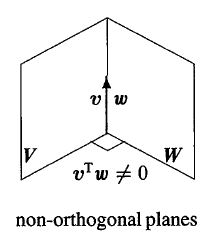
\includegraphics{week5/orthogonality}
\caption{Orthogonality is impossible when $\dim\bm U+\dim\bm V>\dim(\bm U\cup\bm V)$}
\end{figure}
\end{example}
\begin{remark}
When a vector is in two orthogonal subspaces, it \textit{must} be zero. It is \emph{perpendicular} to
itself. 
\\The reason is clear: this vector $\bm u\in\bm U$ and $\bm u\in\bm V$, so $\inp{\bm u}{\bm u}=0$. It has to be zero vector.
\end{remark}
If two subspaces are perpendicular, their basis must be ind.
\begin{theorem}
Assume $\{u_1,\dots,u_k\}$ is the basis for $\bm U$, $\{v_1,\dots,v_l\}$ is the basis for $\bm V.$ If $\bm U\perp\bm V$ ($u_i\perp v_j$ for $\forall i,j$), then $u_1,u_2,\dots,u_k,v_1,v_2,\dots,v_l$ must be ind.
\end{theorem}
\begin{proof}
Suppose there exists $\{\alpha_1,\dots,\alpha_k\}$ and $\{\beta_1,\dots,\beta_l\}$ such that
\[
\alpha_1u_1+\dots+\alpha_ku_k+\beta_1v_1+\dots+\beta_lv_l=\bm 0
\]
then equivalently,
\[
\alpha_1u_1+\dots+\alpha_ku_k=-(\beta_1v_1+\dots+\beta_lv_l).
\]
Then we set $\bm w=\alpha_1u_1+\dots+\alpha_ku_k$, obviously, $\bm w\in\bm U$ and $\bm w\in\bm V$.

 Hence it must be zero (This is due to remark above). Thus we have
\begin{gather*}
\alpha_1u_1+\dots+\alpha_ku_k=\bm 0\\
\beta_1v_1+\dots+\beta_lv_l=\bm 0.
\end{gather*}
Due to the independence, we have $\alpha_i=0$ and $\beta_j=0$ for $\forall i,j$. 
\end{proof}
\begin{corollary}
For subspaces $\bm U$ and $\bm V$, we obtain
\[
\dim(\bm U\cup\bm V)\le \dim(\bm U) + \dim(\bm V).
\]
\end{corollary}
For subspaces $\bm U$ and $\bm V\in\mathbb{R}^{n}$, if $\mathbb{R}^{n}=\bm U\cup\bm V$, and moreover, $n=\dim(\bm U)+\dim(\bm V)$, then we say $\bm V$ is the \emph{orthogonal complement} of $\bm U$.
\begin{definition}[orthogonal complement]
For subspaces $\bm U$ and $\bm V\in\mathbb{R}^{n}$, if $\dim(\bm U)+\dim(\bm V)=n$ and $\bm U\perp\bm V$, then we say $\bm V$ is the \emph{orthogonal complement} of $\bm U$. We denote $\bm V$ as $\bm U^{\perp}$.

Moreover, $\bm V=\bm U^{\perp}$ iff $\bm V^{\perp}=\bm U$.
\end{definition}
\begin{example}
Suppose $\bm U\cup\bm V=\mathbb{R}^{3}$, $\bm U=\Span\{\bm e_1,\bm e_2\}$. If $\bm V$ is the orthogonal complement of $\bm U$, then $\bm V=\Span\{\bm e_3\}$.
\end{example}

Next we study the relationship between the null space and the row space in $\mathbb{R}^n$.
\begin{theorem}[Fundamental theorem for linear alegbra, part 2] Given $\bm A\in\mathbb{R}^{m\times n}$,

\emph{$N(\bm A)$ is the orthogonal complement of the row space of $\bm A$, $\mathcal{C}(\bm A\trans)$ (in $\mathbb{R}^{n}$).}

\emph{$N(\bm A\trans)$ is the orthogonal complement of the column space $\mathcal{C}(\bm A)$ (in $\mathbb{R}^{m}$).}
\end{theorem}
\begin{proof}
\begin{itemize}
\item
Firstly, we show $\dim(N(\bm A))+\dim(\mathcal{C}(\bm A\trans))=n$:

We know that $\dim(N(\bm A))=n-r$ and $\dim(\mathcal{C}(\bm A\trans)) = r$, where $r=\rank(\bm A)$.

Hence $\dim(N(\bm A))+\dim(\mathcal{C}(\bm A\trans))=n$.
\item
Then we show $N(\bm A)\perp \mathcal{C}(\bm A\trans)$:

For any $x\in N(\bm A)$, if we set $\bm A=\begin{bmatrix}
a_1\trans\\a_2\trans\\\vdots\\a_m\trans
\end{bmatrix}$, then we obtain:
\[
\bm{Ax}=\begin{bmatrix}
a_1\trans\\a_2\trans\\\vdots\\a_m\trans
\end{bmatrix}\begin{bmatrix}
\bm x
\end{bmatrix}=\begin{bmatrix}
0\\0\\\vdots\\0
\end{bmatrix}
\]
Hence \textit{every row has a zero product with} $\bm x$, i.e., $\inp{a_i}{\bm x}=0$ for $\forall i\in\{1,2,\dots,m\}$.

For any $y=\sum_{i=1}^m\alpha_ia_i\in \mathcal{C}	(\bm A\trans)$, we obtain:
\[
\begin{aligned}
\inp{\bm x}{y}&=\inp{y}{\bm x}=\inp{\sum_{i=1}^m\alpha_ia_i}{\bm x}\\
&=\sum_{i=1}^{m}\alpha_i\inp{a_i}{\bm x}=0.
\end{aligned}
\]
Hence $\bm x\perp y$ for $\forall \bm x\in N(\bm A)$ and $y\in \mathcal{C}(\bm A\trans)$.\\
\end{itemize}
Hence $N(\bm A)^{\perp}=\mathcal{C}(\bm A\trans)$. Similarly, we have $N(\bm A\trans)^{\perp}=\mathcal{C}(\bm A)$. 
\end{proof}

\begin{corollary}
$\bm{Ax}=\bm b$ is solvable if and only if $\bm y\trans\bm A=\bm 0$ implies $\bm y\trans\bm b$=0.
\end{corollary}
\begin{proof} The following statements are equivalent:
\begin{itemize}
\item
$\bm{Ax}=\bm b$ is solvable.
\item
$\bm b\in \mathcal{C}(\bm A)$.
\item
$\bm b\in N(\bm A\trans)^{\perp}$
\item
$\bm y\trans\bm b=0$ for $\forall y\in N(\bm A\trans)$
\item
Given $\bm y\trans\bm A=\bm 0$, i.e., $y\in N(\bm A\trans)$, it implies $\bm y\trans\bm b=0$.
\end{itemize}
\end{proof}
The \emph{Inverse Negative Proposition} is more commonly useful:
\begin{corollary}
$\bm{Ax}=\bm b$ has no solution if and  and only if $\exists \bm y$ s.t. $\bm y\trans\bm A=0$ and $\bm y\trans\bm b\ne 0$.
\end{corollary}
We could extend this corollary into general case:
\begin{remark}
\begin{theorem}\label{theorem_12.3}
$\bm{Ax}\ge\bm b$ has no solution if and only if $\exists \bm y\ge\bm 0$ such that $\bm y\trans\bm A=\bm 0$ and $\bm y\trans\bm b\ge \bm 0$.
\end{theorem}
$\bm y\trans\bm A=0$ requires that there exists one linear combination of the row space to be zero.

The complete proof for this theorem is not required in this course. We only show the necessity case.
\begin{proof}[Necessity case.]
Suppose $\exists \bm y\ge\bm 0$ such that $\bm y\trans\bm A=\bm 0$ and $\bm y\trans\bm b\ge \bm 0$. Assume there exists $x^{*}$ such that $\bm Ax^{*}\ge\bm b$. By postmultiplying $\bm y\trans$ we have 
\[\bm y\trans\bm Ax^{*}\ge\bm y\trans\bm b>\bm 0
\implies 
\bm 0>\bm 0.
\]
which is a contradiction!
\end{proof}
\end{remark}

\begin{example}
Given the system 
\begin{align}
x_1+x_2&\ge1\label{Eq:6:3}
\\
-x_1&\ge-1\label{Eq:6:4}
\\
-x_2&\ge2\label{Eq:6:5}
\end{align}
Eq.(\ref{Eq:6:3})$\x$1+Eq(\ref{Eq:6:4})$\x$1+Eq.(\ref{Eq:6:5})$\x$1 gives
\[
0\ge 2
\]
which is a contradiction!\\
So the key idea of theorem (\ref{theorem_12.3}) is to construct a linear combination of row space to let it become zero. If the right hand is larger than zero, then this system has no solution.
\end{example}
\begin{remark}
\begin{corollary}
If $\bm A=\bm A\trans$, then $N(\bm A\trans)^{\perp}=\mathcal{C}(A)=\mathcal{C}(\bm A\trans)=N(\bm A)$.
\end{corollary}
\begin{corollary}\label{corollary_12.5}
The system $\bm{Ax}=\bm b$ may not have a solution, but $\bm A\trans\bm A\bm x=\bm A\trans\bm b$ always have at least one solution for $\forall\bm b$.
\end{corollary}
\begin{proof}
Since $\bm A\trans\bm A$ is symmetric, we have $\mathcal{C}(\bm A\trans\bm A)=\mathcal{C}(\bm A\bm A\trans)$. Show by yourself that $\mathcal{C}(\bm A\bm A\trans)=\mathcal{C}(\bm A\trans)$, hence $\mathcal{C}(\bm A\trans\bm A)=\mathcal{C}(\bm A\trans)$.

For any vector $\bm b$, we have $\bm A\trans\bm b\in \mathcal{C}(\bm A\trans)\implies\bm A\trans\bm b\in \mathcal{C}(\bm A\trans\bm A)$, which means there exists a linear combination of the columns of $\bm A\trans\bm A$ that equals to $\bm b$.

Or equivalently, there exists a solution to $\bm A\trans\bm A\bm x=\bm A\trans\bm b$.
\end{proof}
\begin{corollary}\label{corollary_12.6}
$\bm A\trans\bm A$ is invertible if and only if $\bm A$ is full column rank, i.e., columns of $\bm A$ are ind.
\end{corollary}
\begin{proof}
We have shown that $C(\bm A\trans\bm A)=C(\bm A\trans)$.

Hence $C(\bm A\trans\bm A)^{\perp}=C(\bm A\trans)^{\perp}\implies N(\bm A\trans\bm A)=N(\bm A)$.

Thus, the following statements are equivalent:
\begin{itemize}
\item
$\bm A$ has ind. columns
\item
$N(\bm A)=\{\bm 0\}$
\item
$N(\bm A\trans\bm A)=\{\bm 0\}$
\item
$\bm A\trans\bm A$ is invertible.
\end{itemize}
\end{proof}
\end{remark}
\subsection{Least Squares Approximations}
The linear system $\bm{Ax}=\bm b$ often has no solution, if so, what should we do?

We cannot always get the error $\bm e=\bm b-\bm{Ax}$ down to zero, so we want to use \textit{least square method} to minimize the error. In other words, our goal is to
\[
\min_{\bm x\in\mathbb{R}^n}\bm e^2:=\min_{\bm x}\|\bm{Ax}-\bm b\|^2=\sum_{i=1}^{m}(a_i\trans\bm x-b_i)^2
\]
where $\bm A\in\mathbb{R}^{m\times n}$ and $\bm b\in\mathbb{R}^m$. The minimizer $\bm x$ is called the \emph{linear least squares solution}.

\subsubsection{Least Squares by Convex Optimization}
Firstly, you should know some basic calculus knowledge for matrix:
\paragraph{The Chian Rule} Given two vectors $f(x),g(x)$ of appropriate size,
\[
\frac{\partial(f\trans g)}{\partial x}=\frac{\partial f(x)}{\partial x}g(x)+\frac{\partial g(x)}{\partial x}f(x)
\]
\paragraph{Examples of Matrix Derivative}
\begin{align}
\frac{\partial(a\trans \bm x)}{\partial \bm x}&=a\\
\frac{\partial(a\trans \bm A\bm x)}{\partial \bm x}&=\frac{\partial((\bm A\trans a)\trans\bm x)}{\partial \bm x}=\bm A\trans a\\
\frac{\partial(\bm A\bm x)}{\partial \bm x}&=\bm A\trans\\
\frac{\partial(\bm x\trans\bm A\bm x)}{\partial \bm x}&=\bm A\bm x+\bm A\trans\bm x
\end{align}

Thus, in order to minimize $\|\bm{Ax}-\bm b\|^2=(\bm{Ax}-\bm b)\trans(\bm{Ax}-\bm b)$, it suffices to let its \emph{derivative} with respect to $\bm x$ to be \emph{zero.} (Since $\|\bm{Ax}-\bm b\|^2$ is convex, which will be discussed in detail in other courses.) Hence we have:
\[\begin{aligned}
\frac{\partial (\bm{Ax}-\bm b)\trans(\bm{Ax}-\bm b)}{\partial \bm x}&=\frac{\partial(\bm{Ax}-\bm b)}{\partial \bm x}(\bm{Ax}-\bm b)+\frac{\partial(\bm{Ax}-\bm b)}{\partial \bm x}(\bm{Ax}-\bm b)\\
&=2\frac{\partial(\bm{Ax}-\bm b)}{\partial \bm x}(\bm{Ax}-\bm b)\\
&=2(\frac{\partial(\bm A\bm x)}{\partial \bm x}-\frac{\partial(\bm b)}{\partial \bm x})(\bm{Ax}-\bm b)\\
&=2\bm A\trans(\bm{Ax}-\bm b)=\bm 0.
\end{aligned}
\]
Or equivalently, 
\[
\bm A\trans\bm{Ax}=\bm A\trans\bm b.
\]
According to corollary (\ref{corollary_12.5}), this equation always exists a solution. This equation is called the \emph{normal equation}.
\begin{theorem}\label{theorem_12.4}
A vector $\bm x_{\text{LS}}$ is an optimal solution to the least squares problem
\begin{subequations}
\begin{equation}
\min_{\bm x\in\mathbb{R}^n}\|\bm b-\bm{Ax}\|_2^2
\end{equation}
if and only if it satisfies
\begin{equation}
\bm A\trans\bm A\bm x_{\text{LS}} = \bm A\trans\bm b.
\end{equation}
\end{subequations}
\end{theorem}
\subsubsection{Fit a stright line}
Given a collection of data $(\bm x_i,y_i)$ for $i=1,\dots,m$, we can use a stright line to fit these points:
\[
\left\{
\begin{aligned}
y_1&=a_0+a_1x_{1,1}+a_2x_{1,2}+\dots+a_nx_{1,n}+\varepsilon_1\\
y_2&=a_0+a_1x_{2,1}+a_2x_{2,2}+\dots+a_nx_{2,n}+\varepsilon_2\\
\vdots\\
y_m&=a_0+a_1x_{m,1}+a_2x_{m,2}+\dots+a_nx_{m,n}+\varepsilon_m
\end{aligned}
\right.
\]
Our fit line is 
\[
\hat y=a_0+a_1x_1+a_2x_2+\dots+a_nx_n
\]
In \textit{compact matrix form}, we have
\[
\begin{bmatrix}
y_1\\y_2\\\vdots\\y_n
\end{bmatrix}
=\begin{bmatrix}
1&x_{1,1}&x_{1,2}&\dots&x_{1,n}\\
1&x_{2,1}&x_{2,2}&\dots&x_{2,n}\\
\vdots&\vdots&&&\\
1&x_{m,1}&x_{m,2}&\dots&x_{m,n}\\
\end{bmatrix}\begin{bmatrix}
a_0\\a_1\\a_2\\\vdots\\a_{n}
\end{bmatrix}+\begin{bmatrix}
\varepsilon_1\\\varepsilon_2\\\vdots\\\varepsilon_m
\end{bmatrix}
\]
Or equivalently, we have 
\[
\bm y=\bm{Ax}+\bm \varepsilon
\]
where $\bm A =\begin{bmatrix}
1&x_{1,1}&x_{1,2}&\dots&x_{1,n}\\
1&x_{2,1}&x_{2,2}&\dots&x_{2,n}\\
\vdots&\vdots&&&\\
1&x_{m,1}&x_{m,2}&\dots&x_{m,n}\\
\end{bmatrix}_{m\times (n+1)}$, $\bm x=\begin{bmatrix}
a_0\\a_1\\a_2\\\vdots\\a_{n}
\end{bmatrix}_{(n+1)\times 1}$, $\bm \varepsilon=\begin{bmatrix}
\varepsilon_1\\\varepsilon_2\\\vdots\\\varepsilon_m
\end{bmatrix}_{m\times 1}$.\\
Our goal is to minimize $\|\hat{\bm y}-\bm y\|^2=\|\bm{Ax}-\bm y\|^2$. Then by theorem (\ref{theorem_12.4}), it suffices to sovle $\bm A\trans\bm A\bm x=\bm A\trans\bm y$.

\subsection{Projections}
In corollary (\ref{corollary_12.6}), we know that if $\bm A$ has ind. columns, then $\bm A\trans\bm A$ is invertible. On this condition, the normal equation $\bm A\trans\bm A\bm x=\bm A\trans\bm b$ has the unique solution $\bm x^{*}=(\bm A\trans\bm A)^{-1}\bm A\trans\bm b$, which follows that the error $\bm b-\bm A\bm x^{*}$ is minimized. Note that $\bm A\bm x^{*}=\bm A(\bm A\trans\bm A)^{-1}\bm A\trans\bm b$ is \emph{approximately} equal to $\bm b$. 
\begin{itemize}
\item
If $\bm b$ and $\bm{A}\bm x^{*}$ are exactly in the same space, i.e., $\bm b\in\mathcal{C}(\bm A)$, then $\bm{A}\bm x^{*}=\bm b$. The error is equal to zero.
\item
Otherwise, just as the Figure (\ref{figure_12.2}) shown, $\bm A\bm x^{*}$ is the projection of $\bm b$ to subspace $\mathcal{C}(\bm A)$.
\end{itemize}
\begin{figure}[t]
\centering
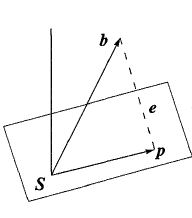
\includegraphics{week5/projection}
\caption{The projection of $\bm b$ onto a subspace $\bm S:=\mathcal{C}(\bm A)$.}\label{figure_12.2}
\end{figure}
\begin{definition}[Projection]
Let $\bm S\in\mathbb{R}^{m}$ be a non-empty closed set and $\bm b\in\mathbb{R}^m$ be given. Then the projection of $\bm b$ onto the set $\bm S$ is the solution to
\[
\min_{\bm z\in\bm S}\|\bm z-\bm b\|_2^2,
\]
where we use notation $\Proj_{\bm S}(\bm b)$ to denote the projection of $\bm b$ onto $\bm S$.
\end{definition}
By definition, the projection of $\bm b$ onto the subspace $\mathcal{C}(\bm A)$ is given by 
\[
\Proj_{\mathcal{C}(\bm A)}(\bm b):=\bm A\bm x^*,\quad
\text{where }\bm x^*=\arg\min_{\bm x\in\mathbb{R}^n}\|\bm{Ax} - \bm b\|.
\]

\begin{definition}[Projection matrix]
Given the projection
\[
\Proj_{C(\bm A)}(\bm b):=\bm A\bm x^{*}=\bm A(\bm A\trans\bm A)^{-1}\bm A\trans\bm b,
\]
since $[\bm A(\bm A\trans\bm A)^{-1}\bm A\trans]\bm b$,
we call the projection operator $\bm P:=\bm A(\bm A\trans\bm A)^{-1}\bm A\trans$ as the \emph{projection matrix} of $\bm A$.
\end{definition}
\begin{definition}[Idempotent]
Let $\bm A$ be a \emph{square} matrix that satisfies $\bm A=\bm A\bm A$, then $\bm A$ is called an \emph{idempotent} matrix.
\end{definition}
Let's show that the projection matrix is \textit{idempotent}:
\[
\begin{aligned}
\bm P^{2}&=\bm A(\bm A\trans\bm A)^{-1}\bm A\trans\bm A(\bm A\trans\bm A)^{-1}\bm A\trans\\
&=\bm A(\bm A\trans\bm A)^{-1}(\bm A\trans\bm A)(\bm A\trans\bm A)^{-1}\bm A\trans\\
&=\bm A(\bm A\trans\bm A)^{-1}\bm A\trans=\bm P.
\end{aligned}
\]

\subsubsection{Observations}
\begin{itemize}
\item
Suppose $\bm b\in \mathcal{C}(\bm A)$, i.e., $\exists \bm x$ s.t. $\bm{Ax}=\bm b$. Then the projection of $\bm b$ is exactly $\bm b$:
\[
\begin{aligned}
\bm{Pb}&=\bm A(\bm A\trans\bm A)^{-1}\bm A\trans(\bm b)\\
&=\bm A(\bm A\trans\bm A)^{-1}\bm A\trans(\bm{Ax})\\
&=\bm A(\bm A\trans\bm A)^{-1}(\bm A\trans\bm A)\bm x\\
&=\bm{Ax}=\bm b.
\end{aligned}
\]
\item
Assume $\bm A$ has only one column, say, $\bm a$. Then we have
\[\begin{aligned}
\bm x^{*}&=(\bm A\trans\bm A)^{-1}\bm A\trans\bm b=\frac{\bm a\trans\bm b}{\bm a\trans\bm a}\\
\bm A\bm x^{*}&=\bm{Pb}=\bm A(\bm A\trans\bm A)^{-1}\bm A\trans(\bm b)=\frac{\bm a\trans\bm b}{\bm a\trans\bm a}\times\bm a=\frac{\bm a\trans\bm b}{\|\bm a\|^2}\times\bm a
\end{aligned}
\]
More interestingly, 
\[\frac{\bm a\trans\bm b}{\|\bm a\|^2}\times\bm a=\frac{\|\bm a\|\|\bm b\|\cos\theta}{\|\bm a\|^2}\times\bm a=\|\bm b\|\cos\theta\times\frac{\bm a}{\|\bm a\|}\]
which is the projection of $\bm b$ onto a line $\Span\{\bm a\}$. (Shown in figure (\ref{Fig:6:3}).)
\begin{figure}[H]
\centering
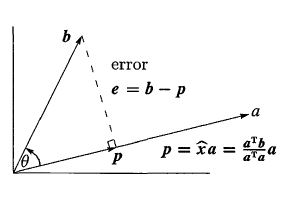
\includegraphics[width=10cm]{week5/projection_line}
\caption{The projection of $\bm b$ onto a line $\bm a$.}
\label{Fig:6:3}
\end{figure}
More generally, we can write the projection of $\bm b$ onto the line $\Span\{\bm a\}$ as:
\[
\Proj_{\Span\{\bm a\}}(\bm b)=\frac{\inp{\bm a}{\bm b}}{\inp{\bm a}{\bm a}}\bm a
\]
\paragraph{Changing an Orthogonal Basis}
Note that the error $\bm b-\Proj_{\Span\{\bm a\}}(\bm b)$ is perpendicular to $\bm a$, and $\bm b-\Proj_{\Span\{\bm a\}}(\bm b)\in\Span\{\bm a,\bm b\}.$

If we define $\bm b'=\bm b-\Proj_{\Span\{\bm a\}}(\bm b)$, then it's easy to check that $\Span\{\bm a,\bm b'\}=\Span\{\bm a,\bm b\}$ and $\bm a\perp\bm b'$. 

Hence, we convert the basis $\{\bm a,\bm b\}$ into another basis $\{\bm a,\bm b'\}$ such that the elements are orthogonal to each other. For general subspace we could also use this approach to obtain an orthogonal basis, which will be discussed in next lecture. 
\end{itemize}









%\section{Friday}\index{week7_Thursday_lecture}

\subsection{Polynomials}
\begin{definition}[polynomial]
Let $k$ be a field, and $f=\sum_{i=0}^nc_ix^i$ be a polynomial in $k[x]$. An element $a\in k$ is a root of $f$ if
\[
f(a)=\sum_{i=0}^nc_ia^i=0
\]
in $k$.
\end{definition}
question: what is $k[x]$?
\begin{corollary}
For all $f\in k[x]$, $a\in k$, then there exists $q\in k[x]$ such that
\[
f=q(x-a)+f(a)
\]
\end{corollary}
\begin{proof}
By division theorem, there exists $q,r\in k[x]$ such that
\[
f=q\cdot (x-a)+r,\quad
\mbox{deg}r<\mbox{deg}(x-a)=1
\]
which implies $r$ is a constant. Evaluate both sides for $x=a$, we have
\[
f(a)=r.
\]
\end{proof}
\begin{proposition}[root theorem]
Let $k$ be a field, $f$ a polynomial is $k[x]$. Then $a\in k$ is a root of $f$ iff $(x-a)$ divides $f$ in $k[x]$.
\end{proposition}
\begin{proof}
For forward direction, there exists $q\in k[x]$ such that
\[
f=q(x-a)+f(a)=q(x-a)\implies (x-a)|f
\]
For the reverse direction, if $f=q(x-a)$ for some $q\in k[x]$, then $f(a)=q(a)(a-a)=0$, i.e., $a$ is a root of $f$.
\end{proof}
\begin{theorem}
Let $k$ be a field, $f$ a nonzero polynomial in $k[x]$
\begin{enumerate}
\item
If $f$ has some degree $n$, then it has at most $n$ roots in $k$
\item
If $f$ has degree $n$ and $a_1,\dots,a_n\in k$ are distinct roots of $f$, then
\[
f=c\prod_{i=1}^n(x-a_i)
\]
for some $c\in k$.
\end{enumerate}
\end{theorem}
\begin{proof}
\begin{enumerate}
\item
We show the first part by induction. Suppose it holds for all nonzero polynomails with degree strictly less than $n$, and $\mbox{deg}f=n$. If $f$ has no roots in $k$, the proof is complete, otherwise suppose a root $a\in k$. There exists $q\in k[x]$ such that
\[
f=q(x-a)
\]
For the any other root $b\in k$, we have 
\[
0=q(b)(b-a)
\]
Since $k$ is a firld, it has no zero divisors, which implies $q(b)=0$, since $b-a\ne0$. Thus $b$ is a root of $q$. Since $\mbox{deg}q<n$, by induction we imply $q$ has at most $n-1$ roots, i.e., $f$ has at most $n-1$ roots that are different from $a$.
\item
If $n=1$, then $f=c_0+c_1x$ for some $c_i\in k$ with $c_1\ne0$, which implies
\[
0=f(a_1)=c_0+c_1a_1\implies c_0=-c_1a_1\implies
f=-c_1a_1+c_1x=c_1(x-a_1)
\]
Suppose $n>1$, and the claim holds for all $n'\in\mathbb{N}$ such that $n'<n$. By previuos claim, there exists $q\in k[x]$ such that
\[
f=q(x-a_n)
\]
Since $\mbox{deg}q=n-1$, and for $1\le i<n$, we have
\[
0=f(a_i)=q(a_i)(a_i-a_n)\implies q(a_i=0),
\]
which implies $a_1,\dots,a_{n-1}$ are $n-1$ distinct roots of $q$ as well. Thus there exists $c\in k$ s.t.
\[
q=c(x-a_1)\cdots(x-a_{n-1}),
\]
which follows that
\[
f=q(x-a_n)=c(x-a_1)\cdots(x-a_n)
\]
\end{enumerate}
\end{proof}

\begin{corollary}
Let $k$ be a field. Let $f,g$ be nonzero polynomails in $k[x]$. Let $n=\max\{\mbox{deg}f,\mbox{deg}g\}$. If $f(a)=g(a)$ for $n+1$ distinct $a\in k$, then $f=g$.
\end{corollary}
\begin{proof}
Let $h=f-g$, then $\mbox{deg}h\le n$. There are $n+1$ distinct elements $a\in k$ s.t. $h(a)=0$. If $h\ne0$, then it is a nonzero polynomial of degree $\le n$ which has $n+1$ distinct roots, which is a constraction. $h=0$ implies $f=g$.
\end{proof}
\begin{definition}
A polynomail in $k[x]$ is called a \emph{monic polynomial} if its leading coefficient is $1$.
\end{definition}
\begin{theorem}
Let $k$ be a field, then the ring $k[x]$ is a PID.
\end{theorem}
\begin{corollary}
Let $k$ be a field, and $f,g$ be nonzero polynomials in $k[x]$. There exists a unique monic polynomial $d\in k[x]$ with the following properties:
\begin{enumerate}
\item
$(f,g)=(d)$
\item
$d$ divides both $f$ and $g$, i.e., there exists $a,b\in k[x]$ s.t. $f=ad,g=bd$
\item
There are polynomials $p,q\in k[x]$ such that $d=pf+qg$
\item
If $h\in k[x]$ is a divisor of $f,g$, then $h$ divides $d$.	
\end{enumerate}
This $d\in k[x]$ is called the \emph{greatest common divisor} (GCD) of $f$ and $g$. We say $f$ and $g$ are \emph{relatively prime} if their GCD is 1.
\end{corollary}
\begin{proof}
By the PID theorem, there exists $d=\sum_{n=0}^\infty a_ix^i\in k[x]$ such that $(d)=(f,g)$. Replacing $d$ with $a_n^{-1}d$, we assume $d$ is a monic polynomial. It remains to show that $d$ is unique. 

Suppose $(d)=(d')$, there exists nonzero $p,q\in k[x]$ such that
\[
d'=pd,\quad
d=qd'
\]
which follows that
\[
\mbox{deg}d'=\mbox{deg}d+\mbox{deg}p,\quad
\mbox{deg}d=\mbox{deg}q+\mbox{deg}d'=\mbox{deg}q+\mbox{deg}d+\mbox{deg}p,
\]
i.e., $\mbox{deg}p=\mbox{deg}q=0$. Thus $\mbox{deg}d=\mbox{deg}d'$. Comparing the leading coefficients of $d'$ and $pd$, we have $p=1$, i.e., $d=d'$.

The remaining part follows similarly.
\end{proof}
\begin{definition}[Irreducible]
Let $R$ be a commutative ring. A non-zero element $p\in R$ which is not a unit is said to be \emph{irreducible} if $p=ab$ implies that either $a$ or $b$ is a unit.
\end{definition}
\begin{example}
The set of irreducible elements in the ring $\mathbb{Z}$ is
\[
\{\pm p\mid p\mbox{ is a prime number}\}
\]
\end{example}
Let $k$ be a field.
\begin{proposition}
A polynomial $f\in k[x]$ is a unit iff it is a \emph{nonzero} constant polynomial.
\end{proposition}
\begin{proposition}
A nonzero nonconstant polynoimial $p\in k[x]$ is \emph{irreducible} iff there is no $f,g\in k[x]$ with $\mbox{deg}f,\mbox{deg}g<\mbox{deg}p$, such that $fg=p$.
\end{proposition}
\begin{proof}
\begin{enumerate}
\item
Suppose $p$ is irreducible, and $p=fg$ for some $f,g\in k[x]$ such that $\mbox{deg}f,\mbox{deg}g<\mbox{deg}p$. Then $p=fg$ implies that $\mbox{deg}f,\mbox{deg}g$ are both positive. By previous lemma, both $f,g$ are non-units, which is a contradiction.
\item
Conversely, suppose $p$ is a nonzero non-unit in $k[x]$, which is not equal to $fg$ for $\forall f,g\in k[x]$ with $\mbox{deg}f,\mbox{deg}g<\mbox{deg}p$. Then $p=ab$ for $a,b\in k[x]$ implies that either $a$ or $b$ must have the same degree as $p$, and the otehr factor must be a nonzero constant, i.e., a unit in $k[x]$. Thus $p$ is irreducible.
\end{enumerate}
\end{proof}

\begin{proposition}[Euclid's Lemma]
Let $k$ be a field. Let $f,g$ be polynomials in $k[x]$. Let $p$ be an irreducible polynomial in $k[x]$. If $p|fg$ in $k[x]$, then $p|f$ or $p|g$.
\end{proposition}
\begin{proof}
Suppose $p$ not divides $f$, then any \emph{common divisor} of $p$ and $f$ must have degree strictly less than $\mbox{deg}p$. Since $p$ is irreducible, this implies that any common divisor of $p$ and $f$ is a nonzero constant. Thus the GCD of $p$ and $f$ is 1. There exists $a,b\in k[x]$ such that
\[
ap+bf=1\implies
apg+bfg=g
\]
Since $p$ divides the LHS, it also divides the RHS.
\end{proof}
\begin{proposition}
If $f,g\in k[x]$ are relatively prime, and both divide $h\in k[x]$, then $fg|h$.
\end{proposition}
question
\begin{theorem}[Unique Factorization]
Let $k$ be a field. Every non-constant polynomial $f\in k[x]$ may be written as
\[
f=cp_1\cdots p_n
\]
where $c$ is a non-zero constant, and each $p_i$ is a monic irreducible polynomials in $k[x]$. The factorization is \emph{unique} up to the ordering of the factors.
\end{theorem}
\begin{proof}
Similar to the proof of unique factorization for $\mathbb{Z}$
\end{proof}
\begin{theorem}
Let $k$ be a field, $p$ be a polynomial in $k[x]$. The following statements are equivalent:
\begin{enumerate}
\item
$k[x]/(p)$ is a field
\item
$k[x]/(p)$ is an integral domain
\item
$p$ is irreducible in $k[x]$.
\end{enumerate}
\end{theorem}
\begin{proof}
\begin{enumerate}
\item
(2) implies (3): If $p$ is not irreducible, then there exists $f,g\in k[x]$ with degree strictly less than that of $p$, such that $p=fg$.

It's clear that $p$ does not divide $f$ or $g$ in $k[x]$. The equivalence classes $\bar f$ and $\bar g$ of $f$ and $g$, respectively, modulo $(p)$ is not equal to zero in $k[x]/(p)$. (question) On the other hand, $\bar f\cdot\bar g=\bar{fg}=\bar p=0$ in $k[x]/(p)$, which implies that $k[x]/(p)$ is not an integral domain, which is a contradction.
\item
(3) implies (1): By definiton, the multiplicative identity $1$ of a field is different from addictive identity $0$. We first check that the equivalence lcass $1\in k[x]$ in $k[x]/(p)$ is not zero. Since $p$ is irreducible, we have $\mbox{deg}p>0$, and $1\notin(p)$. Therefore $1+(p)\ne 0+(p)$ in $k[x]/(p)$.

Next, we need to show the existence of multiplicative inverse of any nonzero element in $k[x]/(p)$. Given any $f\in k[x]$ whose equivalence $\bar f$ modulo $(p)$ is nonzero in $k[x]/(p)$, we want to constracut $\bar{f}^{-1}$. Since $\bar{f}\ne0$ in $k[x]/(p)$, we have $f-0\notin(p)$, i.e., $p$ does not divide $f$. Since $p$ is irreducible, we have $gcd(p,f)=1$. There exists $g,h\in k[x]$ such that $fg+hp=1$. Thus $\bar{f}^{-1}=\bar{g}$. This is becasue $fg-1=hp$ implies $fg-1\in(p)$, i.e., $\bar{f}\bar{g}=\bar{fg}=1$ in $k[x]/(p)$.


\end{enumerate}
\end{proof}
\subsection{Polynomials over $\mathbb{Z}$ and $\mathbb{Q}$}
\begin{theorem}
Let $f=a_0+a_1x+\cdots+a_nx^n$ be a polynomial in $\mathbb{Q}[x]$, with $a_i\in\mathbb{Z}$. Every rational root $r$ of $f$ in $\mathbb{Q}$ has the form $r=b/c$ $(b,c\in\mathbb{Z})$, where $b|a_0$ and $c|a_n$
\end{theorem}
\begin{proof}
Let $r=b/c$ be a rational root of $f$, where $b,c$ are relatively prime integers. We have
\[
0=\sum_{i=1}^na_i(b/c)^i
\]
Multiplying both sides above equation by $c^n$, we have
\[
0=a_0c^n+a_1c^{n-1}b+\cdots+a_nb^n
\]
or equivalently,
\[
a_0c^n=-(a_1c^{n-1}+\cdots+a_nb^n)
\]
Since $b$ divides the RHS, and $b,c$ are relatively prime, $b$ must divide $a_0$. Similarly,
\[
a_nb^n=-(a_0c^n+\cdots+a_{n-1}cb^{n-1})
\]
It is clear that $c$ divides $a_n$.
\end{proof}
\begin{definition}
A polynomial $f\in\mathbb{Z}[x]$ is said to be \emph{primitive} if the gcd of its coefficients is 1.
\end{definition}
\begin{remark}
Note that if $f$ is monic, i.e., its leading coefficient is 1, then it is primitive. If $d$ is the gcd of the coefficients of $f$, then $\frac{1}{d}f$ is a primitive polynomial in $\mathbb{Z}[x]$.
\end{remark}
\begin{theorem}[Gauss's Lemma]
If $f,g$ are both primitive, then $fg$ is primitive.
\end{theorem}
\begin{proof}
Write $f=\sum_{k=0}^ma_kx^k$ and $g=\sum_{k=0}^nb_kx^k$, then $fg=\sum_{k=0}^{m+n}c_kx^k$, where
\[
c_{k}=\sum_{i+j=k}a_ib_j.
\]
Assume that $fg$ is not primitive, then there exists a prime $p$ such that $p$ divides $c_k$ for $k=0,1,\dots,m+n$. Since $f$ is primitive, there exists smallest $u$ s.t. $a_u$ is not dividible by $p$; similarly, a smallest $v$ s.t. $b_v$ is not divisible by $p$. We have
\[
c_{u+v}=\left(\sum_{i+j=u+v,(i,j)\ne(u,v)}a_ib_j\right)+a_ub_v,
\]
which implies that
\[
a_ub_v=c_{u+v}-
\left(\sum_{i+j=u+v,i<u}a_ib_j\right)
-
\left(\sum_{i+j=u+v,i>u}a_ib_j\right)
\]
By the minimum conditons on $u$ and $v$, each term on the RHS of the above equation is divisible by $p$. Thus $p$ divides $a_u$ and $b_v$, which implies that $p$ divides either $a_u$ or $b_v$, which is a contradiction.
\end{proof}
\begin{proposition}
Every nonzero $f\in\mathbb{Q}[x]$ has a unique factorization:
\[
f=c(f)f_0,
\]
where $c(f)$ is a positive rational number, and $f_0$ is a primitive polynomial in $\mathbb{Z}[x]$.
\end{proposition}
\begin{definition}
The rational number $c(f)$ is called the \emph{content} of $f$.
\end{definition}















%\section{Assignment Seven}\index{Assignment_Seven}
\begin{enumerate}
\item
Here is a wrong ``proof'' that the \textit{eigenvalues of all real matrices are real}:
\[
\bm{Ax}=\lambda\bm x\text{ gives }\bm x\trans\bm A\bm x=\lambda\bm x\trans\bm x
\implies
\lambda=\frac{\bm x\trans\bm A\bm x}{\bm x\trans\bm x}\in\mathbb{R}.
\]
Find the flaw in this reasoning: a hidden assumption that is not justified.
\item
Let $\bm A$ be an $n\x n$ matrix and let $\lambda$ be an eigenvalue of $\bm A$ whose eigenspace has
dimension $k$, where $1<k<n$. Any basis $\{\bm x_1,\dots,\bm x_k\}$ for the eigenspace can be
extended to a basis $\{\bm x_1,\dots,\bm x_n\}$ for $\mathbb{R}^n$. Let $\bm X=\begin{bmatrix}
\bm x_1&\cdots&\bm x_n
\end{bmatrix}\trans$ and $\bm B=\bm X^{-1}\bm A\bm X.$
\begin{enumerate}
\item
Show that $\bm B$ is of the form
\[
\begin{bmatrix}
\lambda\bm I&\bm B_{12}\\
\bm0&\bm B_{22}
\end{bmatrix}
\]
where $\bm I$ is the $k\x k$ identity matrix
\item
Show that $\lambda$ is an eigenvalue of $\bm A$ with multiplicity at least $k$.
\end{enumerate}
\item
Let $\bm x,\bm y$ be nonzero vectors in $\mathbb{R}^n$, $n\ge2$, and let $\bm A=\bm x\bm y\trans$. Show that
\begin{enumerate}
\item
$\lambda=0$ is an eigenvalue of $\bm A$ with $n-1$ linearly independent eigenvectors. Moreover, due to the conclusion of question 2, $0$ is an eigenvalue of $\bm A$ with multiplicity at least $n-1$.
\item
The remaining eigenvalue of $\bm A$ is
\[
\lambda_n=\trace(\bm A)=\bm x\trans\bm y
\]
and $\bm x$ is an eigenvector belonging to $\lambda_n.$
\item
If $\lambda_n=\bm x\trans\bm y\ne0,$ then $\bm A$ is \textit{diagonalizable.}
\end{enumerate}
\item
Suppose an $n\x n$ matrix $\bm A$ has $n$ distinct eigenvalues $\lambda_1,\dots,\lambda_n$. Consider the matrix $\bm B=(\bm A-\lambda_1\bm I)\dots(\bm A-\lambda_n\bm I)$. Prove that $\bm B$ must be a \textit{zero matrix}.\\
\textit{Hint:} How to do eigendecomposition for $\bm A-\lambda_i\bm I$?
\item
Let $\bm A$ and $\bm B$ be $n\x n$ matrices. Show that
\begin{enumerate}
\item
If $\lambda$ is a \emph{nonzero} eigenvalue of $\bm{AB}$, then it is also an eigenvalue of $\bm{BA}$.
\item
If $\lambda=0$ is an eigenvalue of $\bm{AB}$, then $\lambda=0$ is also an eigenvalue of $\bm{BA}$.
\end{enumerate}
\item
\begin{enumerate}
\item
The sequence $a_k$ is defined as
\[
a_0=4,a_1=5,a_{k+1}=3a_k-2a_{k-1},k=1,2,\dots
\]
What is the \textit{general formula} for $a_k$?
\item
The sequence $b_k$ is defined as
\[
b_0=\alpha,b_1=\beta,b_{k+1}=4b_k-4b_{k-1},k=1,2,\dots
\]
What is the \textit{general formula} for $b_k$?\\
\textit{Hint:} Prove the corresponding matrix is similar to
\[
\begin{bmatrix}
2&1\\0&2
\end{bmatrix}.
\]
In order to compute
\[
\begin{bmatrix}
2&1\\0&2
\end{bmatrix}^k,
\]
you need to use the fact that
\[
\text{Given sequence }p_{k+1}=2p_{k}+2^k
\implies
p_k=(p_0+\frac{k}{2})\times2^k.
\]
\end{enumerate}
\item
State and justify whether the following three statements are True or False:
\begin{enumerate}
\item
If $\bm A$ is \textit{real symmetric} matrix, then any 2 linearly independent eigenvectors of $\bm A$ are perpendicular.
\item
Any $n$ by $n$ complex matrix with $n$ real eigenvalues and $n$ orthonormal eigenvectors
is a \textit{Hermitian matrix}.
\item
If $\bm A$ is diagonalizable. then $e^{\bm A}$ is diagonalizable.\\
(We define $e^{\bm A}=\bm I+\bm A+\frac{1}{2!}\bm A^2+\dots$)
\item
If $\bm A$ is Hermitian and $\bm A$ is invertible, then $\bm A^{-1}$ is also Hermitian.
\end{enumerate}
\item
\begin{enumerate}
\item
For a complex $\bm A$, is the left nullspace $N(\bm A\trans)$ orthogonal to $C(\bm A)$ under the old
unconjugated inner product $\bm x\trans\bm y$ or new conjugated inner product $\bm x\Her\bm y$? What about
$N(\bm A\Her)$ and $C(\bm A)$?
\item
For a real vector subspace $V$, the intersection of $V$ and $V^{\perp}$ is only the single point $\{\bm 0\}$. Now suppose $V$ is a complex vector subspace. If we define $V^{\perp}$ as the set of vector $\bm x$ with $\bm x\trans\bm v=0$ for all $\bm v\in V$. Give an example of a $V$ that intersects $V^{\perp}$ at a nonzero vector. What about if we use $\bm x\Her\bm v=0$? Does $V$ ever intersect $V^{\perp}$ at a nonzero vector using the conjugated definition of orthogonality?
\end{enumerate}
\end{enumerate}
%%
\chapter{Week4}

\section{Convergence}\index{week4_Friday_lecture}

\begin{definition}[Convergent]
An infinite sequence $\{z_n\}$ of complex numbers has a limit $z_0$, if for $\forall$ $\varepsilon>0$, there exists a positive integer $n_0$ such that
\[
\begin{array}{ll}
|z_n-z|<\varepsilon,
&
\mbox{whenever }n>n_0
\end{array}
\]
We say the sequence $z_n$ converges to $z$ and write as
\[
\lim_{n\to\infty}z_n=z
\]
When the sequence does not have a limit, then it diverges.
\end{definition}
The uniqueness of limit of a seuqnece is guaranteed.

\begin{proposition}
For $z_n=x_n+iy_n$, we have 
\[
\lim_{n\to\infty}z_n=x+iy
\]
if and only if
\[
\begin{array}{lll}
\lim_{n\to\infty}x_n=x,
&
\mbox{and}
&
\lim_{n\to\infty}y_n=y
\end{array}
\]
\end{proposition}

\begin{definition}[Convergent Series]
An infinite \emph{series} $\sum_{n=1}^\infty z_n$ of complex numbers converges to the sum $S$ if the partial sum sequences
\[
S_N=\sum_{n=1}^Nz_n
\]
converges to $S$, then we write
\[
\sum_{n=1}^\infty z_n=S.
\]
\end{definition}

\begin{proposition}
For $z_n=x_n+iy_n$, we have 
\[
\sum_{n=1}^\infty z_n=X+iY
\]
if and only if
\[
\begin{array}{lll}
\sum_{n=1}^\infty x_n=X
&
\mbox{and}
&
\sum_{n=1}^\infty y_n=Y
\end{array}
\]
\end{proposition}

\begin{proposition}
The series $\sum_{n=1}^\infty z_n$ converges implies that $\lim_{n\to\infty}z_n=0$.
\end{proposition}

\begin{definition}[Absolute Convergence]
The series $\sum_{n=1}^\infty z_n$ is said to be \emph{absolutely convergent} if
\[
\sum_{n=1}^\infty|z_n|
\]
converges, i.e., $\sum_{n=1}^\infty|x_n|$ and $\sum_{n=1}^\infty|y_n|$ converge.
\end{definition}
\begin{proposition}
Absolute convergence implies convergence
\end{proposition}

\begin{definition}[Remainder]
The \emph{remainder} $\rho_N$ of a series after $N$ terms is defined by:
\[
\rho_N=\sum_{n=N+1}^\infty S_n
\]
\end{definition}
\begin{proposition}
A series converges to a number $S$ iff the sequence of remainders tends to zero.
\end{proposition}

It's easy to verifty that
\[
\sum_{n=0}^\infty z_n=\frac{1}{1-z},\qquad\mbox{whenever }|z|<1
\]
with the aid of partial sums and remainders.

\subsection{Taylor Series}
\begin{definition}[Power Series]
The power series has the form
\[
\sum_{n=0}^\infty a_n(z-z_0)^n
\]
\end{definition}

\begin{theorem}[Convergent of Taylor Series]
Suppose $f$ is \emph{analytic} on $|z-z_0|<R$, then 
\begin{equation}
f(z)=\sum_{n=0}^\infty \frac{f^{(n)}(z_0)}{n!}(z-z_0)^n,
\end{equation}
for $|z-z_0|<R$, i.e., $f(z)$ admits its Taylor expansion at $z=z_0$ in this rigion.
\end{theorem}
\begin{remark}
Typically, when $z_0=0$, we say this series is the \emph{Maclaurin series}.
\end{remark}
\begin{proof}
\textbf{Step 1: Applying Cauchy Integral Formula.}
For fixed $z$, let $r:=|z-z_0|<R$ and take $r_0$ such that $r<r_0<R$. Construct a contour $C_0:\{z\in\mathbb{C}\mid |z-z_0|=r_0\}$ in the positive sense, which follows that
\begin{subequations}
\begin{align}
f(z)&=\frac{1}{2\pi i}\int_{C_0}\frac{f(s)}{s-z}\diff s\label{Eq:4:2:b}
\end{align}

\textbf{Step 2: Expand $1/(s-z)$.} With some calculation, we obtain
\begin{align}\label{Eq:4:2}
\frac{1}{s-z}&=\frac{1}{s-z_0}\cdot\frac{1}{1-\frac{z-z_0}{s-z_0}}\\
&=\frac{1}{s-z_0}\left\{1+\frac{z-z_0}{s-z_0}+\cdots+(\frac{z-z_0}{s-z_0})^{N-1}+\frac{(\frac{z-z_0}{s-z_0})^{N}}{1 - \frac{z-z_0}{s-z_0}}\right\}\label{Eq:4:2:d}\\
&=\frac{1}{s-z_0}+\frac{z-z_0}{(s-z_0)^2}+\cdots+\frac{(z-z_0)^{N-1}}{(s-z_0)^N}+\frac{(z-z_0)^N}{(s-z)(s-z_0)^N}\label{Eq:4:2:e}
\end{align}
where $(\ref{Eq:4:2:d})$ is because that
\[
\frac{1}{1-c}=1+c+c^2+\cdots+c^{N-1}+\frac{c^N}{1-c}. 
\]
Substituting (\ref{Eq:4:2:e}) into (\ref{Eq:4:2:b}), we obtain
\begin{align*}
f(z)&=\frac{1}{2\pi i}\int_{C_0}\left\{\frac{f(s)}{(s-z_0)}+\frac{f(s)(z-z_0)}{(s-z_0)^2}+\cdots+\frac{f(s)(z-z_0)^{N-1}}{(s-z_0)^N}+\frac{f(s)(z-z_0)^N}{(s-z)(s-z_0)^N}
\right\}\\
&=f(z_0)+f'(z_0)(z-z_0)+\cdots+\frac{f^{(N-1)}(z_0)}{(N-1)!}(z-z_0)^{N-1}+\rho_N(z)
\end{align*}
with
\begin{equation}\label{Eq:4:2:e}
\rho_N(z)=\frac{(z-z_0)^B}{2\pi i}\int_{C_0}\frac{f(s)}{(s-z)(s-z_0)^N}\diff s
\end{equation}

\textbf{Step 3: Show that $\rho_N(z)$ is convergent.}
\begin{align}
|\rho_N(z)|&\le\frac{|z-z_0|^N}{2\pi}\int_{C_0}\frac{|f(s)|}{|s-z||s-z_0|^N}|\diff s|\\
&\le\frac{r^N}{2\pi}\int_{C_0}\frac{M}{(r_0-r)r_0^N}|\diff s|\\
&=\frac{Mr_0}{r_0-r}\left(\frac{r}{r_0}\right)^N
\end{align}
where we suppose $|f(s)|\le M$ on $C_0$; and $|s-z|\ge|s-z_0| - |z-z_0| = r_0-r$. Therefore,
\[
\rho_N(z)\to0
\]
since $r<r_0$ and $(r/r_0)^N\to0$.
\end{subequations}




\end{proof}

\begin{example}
\begin{enumerate}
\item
For $f(z)=e^z$, which is analytic for $|z-0|<\infty$, thus we have
\[
e^z=\sum_{n=0}^\infty\frac{z^n}{n!},\qquad |z|<\infty
\]
\item
For $f(z)=\sin z=\frac{e^{iz} - e^{-i}}{2i}$, which is analytic for $|z-0|<\infty$, thus we have $f^{(2n)}(0)=0; f^{(2n+1)}(0)=(-1)^n$, and therefore
\[
\sin z=\sum_{n=0}^\infty\frac{(-1)^n}{(2n+1)!}z^{2n+1},\qquad |z|<\infty
\]
\item
For $f(z)=\frac{1}{1-z}$, which is analytic for $|z-0|<1$, we have $f^{(0)}=n!$, and therefore
\[
\frac{1}{1-z}=\sum_{n=0}^\infty\frac{n!}{n!}z^n=\sum_{n=0}^\infty z^n,\qquad |z|<1
\]
\item
For $f(z)=\frac{1}{z}\cdot\frac{1}{1+z}$, we have
\[
\frac{1}{1+z}=\sum_{n=0}^\infty(-z)^n,\qquad |z|<1,
\]
and therefore
\[
\frac{1}{z+z^2}=\frac{1}{z}+\sum_{n=1}^\infty(-1)^nz^{n-1},\qquad 0<|z|<1
\]
\end{enumerate}
\end{example}
\subsection{Laurent Series}
We cannot apply Taylor expansion at a non-analytic point. Fortunately, we can find another series representation for $f(z)$ that involving positive and negative powers of $(z-z_0)$
\begin{definition}[Laurent Series]
The \emph{Laurent series} has the form
\[
\sum_{n=0}^\infty a_n(z-z_0)^n+\sum_{n=1}^\infty\frac{b_n}{(z-z_0)^n}
\]
\end{definition}
\begin{theorem}
Suppose $f$ is analytic throughout an \emph{annular domain} $R_1<|z-z_0|<R_2$. Let $C$ be any \emph{positively oriented simple closed contour} around $z_0$ and lying in that domain. Then
\begin{subequations}
\begin{equation}
f(z)=\sum_{n=0}^\infty a_n(z-z_0)^n+\sum_{n=1}^\infty\frac{b_n}{(z-z_0)^n},\qquad
R_1<|z-z_0|<R_2
\end{equation}
with
\begin{align}
a_n&=\frac{1}{2\pi i}\int_C\frac{f(z)}{(z-z_0)^{n+1}}\diff z,\qquad n=0,1,2,\dots\\
b_n&=\frac{1}{2\pi i}\int_C\frac{f(z)}{(z-z_0)^{-n+1}}\diff z,\qquad n=1,2,\dots
\end{align}
\end{subequations}

\end{theorem}
\begin{remark}
The Laurent series is often written as the form
\[
f(z)=\sum_{n=-\infty}^\infty c_n(z-z_0)^n,\qquad R_1<|z-z_0|<R_2,
\]
where
\[
c_n=\frac{1}{2\pi i}\int_C\frac{f(z)}{(z-z_0)^{n+1}}\diff z,\qquad n=0,\pm1,\pm2,\dots
\]
When $f$ is analytic on $|z-z_0|<R_2$, we have $b_n=0,a_n=\frac{f^{(n)}(z_0)}{n!}$, i.e., the Laurent series reduces to the Taylor series.
\end{remark}
\begin{proof}
\begin{itemize}
\item
For fixed $z$ in the domain, let $r=|z-z_0|$, and construct two positively oriented contours $C_i:\{z\in\mathbb{C}\mid|z-z_0|=r_i\},i=1,2$ such that $R_1<r_1<r<r_2<R_2$. (The reaon why we don't use the boundary is that the function is not analytic on the boundary but only interior to)
\item
Construct a circle $\gamma:\{s\in\mathbb{C}\mid s = z + \delta e^{i\theta},0\le\theta\le2\pi\}$, where the $\delta$ is picked such that $\gamma$ is contained in the interior between $C_1,C_2$. By Cauchy Integral Formula,
\begin{equation}
\int_{C_2}\frac{f(s)\diff s}{s-z}=\int_{C_1}\frac{f(s)\diff s}{s-z}+\int_{\gamma}\frac{f(s)\diff s}{s-z}
\end{equation}
Or equivalently,
\[
f(z)=\frac{1}{2\pi i}\int_{C_2}\frac{f(s)\diff s}{s-z}+\frac{1}{2\pi i}\int_{C_1}\frac{f(s)\diff s}{z-s}
\]
\item
By applying the same trick as (\ref{Eq:4:2}), we have
\begin{subequations}
\begin{equation}
f(z)=\sum_{n=0}^{N-1}a_n(z-z_0)^n+\rho_N(z)+\sum_{n=1}^N\frac{b_n}{(z-z_0)^n}+\sigma_N(z)
\end{equation}
with
\begin{align}
a_n&=\frac{1}{2\pi i}\int_{C_2}\frac{f(s)\diff s}{(s-z_0)^{n+1}}\\
b_n&=\frac{1}{2\pi i}\int_{C_1}\frac{f(s)\diff s}{(s-z_0)^{-n+1}}\\
\rho_N(z)&=\frac{(z-z_0)^N}{2\pi i}\int_{C_2}\frac{f(s)\diff s}{(s-z)(s-z_0)^N}\\
\sigma_N(z)&=\frac{(z-z_0)^{-N}}{2\pi i}\int_{C_1}\frac{f(s)\diff s}{(z-s)(s-z_0)^{-N}}
\end{align}
\end{subequations}
\item
Then we bound the term $\rho_N(z)$ and $\sigma_N(z)$. Suppose $|f(s)|\le M$ on $C_1,C_2$, and note that $|s-z|\ge r_2-r$ for $s\in C_2$; $|z-s|\ge r-r_1$ for $s\in C_1$:
\begin{align*}
\rho_N(z)&\le\frac{Mr_2}{r_2-r}\left(\frac{r}{r_2}\right)^N\\
\sigma_N(z)&\le\frac{Mr_1}{r-r_1}\left(\frac{r_1}{r}\right)^N
\end{align*}
\item
Finally, note that
\begin{align*}
a_n&=\frac{1}{2\pi i}\int_{C}\frac{f(s)\diff s}{(s-z_0)^{n+1}}\\
b_n&=\frac{1}{2\pi i}\int_{C}\frac{f(s)\diff s}{(s-z_0)^{-n+1}}\\
\end{align*}





\end{itemize}
\end{proof}

\begin{example}
\begin{enumerate}
\item
\[
f(z)=\frac{1}{z-1} - \frac{1}{z-2}
\]
This function has two singular points $1,2$. We take $z_0=0$.
\begin{itemize}
\item
When $z\in D_1=\{z:|z|<1\}$, we obtain the Taylor expansion:
\[
f(z)=-\sum_{n=0}^\infty z^n+\sum_{n=0}^\infty\frac{z^n}{2^{n+1}}=\sum_{n=0}^\infty(2^{-n-1}-1)z^n
\]
\item
When $z\in D_2=\{z:1<|z|<2\}$, we obtain the Laurent series:
\[
f(z)=\sum_{n=0}^\infty\frac{z^n}{2^{n+1}}+\sum_{n=1}^\infty\frac{1}{z^n}
\]
\item
When $z\in D_3=\{z:|z|>2\}$, we obtain
\[
f(z)=\sum_{n=1}^\infty\frac{1-2^{n-1}}{z^n}
\]
\end{itemize}
\item
Expand $f(z)=\frac{-z}{(z-1)(z-3)}$ near $z_0=1$, and find the domain of expansion.

The expansion should be the laurent series with domain of expansion $0<|z-1|<2$.
\[
f(z)=\frac{1/2}{z-1}-\frac{3/2}{z-3}=\frac{1/2}{z-1}+\sum_{n=0}^\infty\frac{3}{2^{n+2}}(z-1)^n
\]





\end{enumerate}
\end{example}
\subsection{Power Series}
For power series
\begin{equation}\label{Eq:4:6}
\sum_{n=0}^\infty a_n(z-z_0)^n
\end{equation}
, first we study the range of its convergence.
\begin{theorem}\label{The:4:3}
If the power series (\ref{Eq:4:6}) converges at $z=z_1(\ne z_0)$, then it is \emph{absolutely convergent} at each point in the disk $|z-z_0|<|z_1-z_0|$.
\end{theorem}
\begin{proof}
For any point $z$ around the disk, we have, we have
\[
\left|\frac{z-z_0}{z_1-z_0}\right|:=q<1,
\]
which follows that
\[
|a_n(z-z_0)^n|=|a_n(z_1-z_0)^n|\left|\frac{z-z_0}{z_1-z_0}\right|^n\le Mq^n,
\]
where $|a_n(z_1-z_0)^n|\le M$ since $z_1$ makes the series convergent. By Comparison test, we conclude (\ref{Eq:4:6}) is absolutely convergent.
\end{proof}
\begin{definition}[Uniform convergence]
The series (\ref{Eq:4:6}) is said to be \emph{uniformly convergent} for $|z-z_0|<R$ if as $N\to\infty$,
\[
\sup_{|z-z_0|<R}|\rho_N(z)|\to0
\]
\end{definition}

\begin{theorem}
If the power series (\ref{Eq:4:6}) converges at $z=z_1(\ne z_0)$, then it must be uniformly convergent for any closed circle $|z-z_0|\le \rho$ ($\rho<|z_1-z_0|$).
\end{theorem}
\begin{proof}
Notice that for any $\rho<|z_1-z_0|$, for any $z$ in that closed circle, we have
\[
|a_n(z-z_0)^n|\le |a_n\rho^n|
\]
Due to the conclusion in Theorem(\ref{The:4:3}), we conclude $\sum_{n=1}^\infty |a_n|\rho^n$ is convergent, and therefore $(\ref{Eq:4:6})$ is uniformly convergent.

\end{proof}
Now we are curious about whether the power series is analytic. First we show under which condition does the power series is continuous.
\begin{theorem}
The series (\ref{Eq:4:6}) represents a continuous function at each point inside the circle of convergence.
\end{theorem}

\begin{theorem}
The sum $S(z)$ of power series is analytic at each point $z$ interior to the circle convergence of that series.
\end{theorem}






















%
\chapter{Week2}
\section{Monday}\index{week2_Tuesday_lecture}
\subsection{Reviewing and Announments}
Tutorial: Thursday 7:00pm -9:00pm, ChengDao 208

Homework is due every Monday.

The first homework has been uploaded.

To proof the optimality condition in $\mathbb{R}^n$, we set $h(t) = f(x^*+td)$ for fixed $x^*$ and $d$. It follows that
\[
h'(t)=\nabla\trans f(x^*+td)d
\]
and
\[
h''(t)=d\trans\nabla^2f(x^*+td)d
\]
By the optimality condition for $\mathbb{R}$, we derive the necessary condition:
\[
\left\{
\begin{aligned}
\mbox{$h'(0)=\nabla\trans f(x^*)d=0$ for $\forall d$}\implies \mbox{$\nabla f(x^*)=0$;}\\
\mbox{$h''(0)=d\trans\nabla^2f(x^*)d=0$ for $\forall d$}
\implies
\mbox{$\nabla^2f(x^*)\succeq0$}
\end{aligned}
\right.
\]
together with the sufficient condition:
\[
\left\{
\begin{aligned}
\mbox{$\nabla f(x^*)=0$;}\\
\mbox{$\nabla^2f(x^*)\succ0$}
\end{aligned}
\right.
\]
\subsection{Quadratic Function Case Study}
Given a quadratic function 
\[
f(\bm x) =\frac{1}{2}\bm x\trans\bm Q\bm x+\bm b\trans\bm x
\]
w.l.o.g., assume the matrix $\bm Q$ is symmetric (recall the quadratic section studied in linear algebra).


\begin{definition}[Stationarity]
A point $\bm x^*$ is said to be the stationary point of $f(\bm x)$ if $\nabla f(\bm x^*)=\bm0$.
\end{definition}
To minimize such a function without constraint, we apply the optimality condition:
\begin{enumerate}
\item
The first order optimality condition is given by:
\[
\nabla f(\bm x) = \bm Q\bm x+\bm b=\bm0
\]
The stationary point of the quadratic function $f(\bm x)$ exists iff $\bm b\in\mathcal{C}(\bm Q).$
\item
The second order necessary condition should be:
\[
\nabla^2 f(\bm x)=\bm Q\succeq0
\]
\end{enumerate}
For this special case, if $\bm Q\succeq0$, then $f(\bm x)$ is convex, the solutions to $\nabla f(\bm x) =\bm0$ are local minimum points. Furthermore, they are global minimum points (prove by Taylor Expansion). However, for general functions, we cannot obtain such good results.

\paragraph{Least Squares Problem} Such a problem has been well-studied in statistics given by:
\[
\min_{\bm x}f(\bm x):=\frac{1}{2}\|\bm{Ax}-\bm b\|_2^2
\]
The first order derivative of the minimizer should satisfy:
\[
\nabla f(\bm x)=\bm A\trans(\bm A\bm x-\bm b)
\]
Note that $\bm A\trans\bm b\in\mathcal{C}(\bm A\trans\bm A)$, thus the least squares problem always has a solution. However, such a solution is not unique unless $\bm A$ is full rank.
\paragraph{A Non-trival Quadratic Function}
To minimize the function
\[
f(x,y)=\frac{1}{2}(\alpha x^2+\beta y^2)-x
\] 
We take the first order derivative to be zero:
\[
\nabla f(x,y)=\begin{bmatrix}
\alpha x-1\\\beta y
\end{bmatrix}=\bm0
\]
The second order derivative is given by:
\[
\nabla^2 f(x,y)=\begin{bmatrix}
\alpha&0\\0&\beta
\end{bmatrix}
\]
The optimal solutions depend on the value of $\alpha$ and $\beta$: (although we haven't introduce the definition for convex formally)
\begin{itemize}
\item
If $\alpha,\beta>0$, then this problem is \emph{strongly convex}. By the necessary and sufficient optimality condition for convex problem, we find that $(\frac{1}{\alpha},0)$ is the unique local minimum (It is also the global minimum by plotting the figure).
\item
If $\alpha=0$, this problem has no solution. The objective value $f(x,y)\to-\infty$ as $x\to
\infty$.
\item
If $\beta=0,\alpha>0$, this problem is convex.  By the necessary and sufficient optimality condition for convex problem, $\{(\frac{1}{\alpha},\xi)\mid \xi\in\mathbb{R}\}$ is the set of local minimum. (By plotting the graph, we find that such set is the set of global minimum points)
\item
For $\alpha>0,\beta<0$ case, this problem is non-convex. Actually, $f(x,y)\to-\infty$ as $y\to
\infty$. Hence, this problem has no global minimum point.
\end{itemize}

\paragraph{A Non-trival Function Study}
To minimize the function
\[
\begin{array}{ll}
\min&f(\bm y)=e^{y_1}+\cdots+e^{y_n}\\
\mbox{such that}&y_1+\cdots+y_n=S
\end{array}
\]
We can transform such a constrainted optimization problem into unconstrainted. Let $y_n=S-y_1-\cdots-y_{n-1}$ and substitute it into the objective function, it suffices to solve
\[
\min e^{y_1}+\cdots+e^{y_{n-1}}+e^{S-y_1-\cdots-y_{n-1}}
\]
The stationary point should satisfy:
\[
e^{y_i}=e^{S-y_1-\cdots-y_{n-1}},
\qquad
i=1,2,\dots,n-1
\]
Or equivalently, $y_1=y_2=\cdots=y_{n-1}=y_n$. Hence we derive the unique stationary point:
\[
y_1^*=y_2^*=\cdots=y_n^*=\frac{S}{n}
\]
The value on the stationary point is $f(y^*)=ne^{S/n}$. By checking the second order sufficient optimality condition,
\[
\frac{f}{\partial y_i\partial y_j}=\left\{
\begin{aligned}
e^{y_i}+e^{S-y_1-\cdots-y_{n-1}}&\quad i=j\\
e^{s-y_1-\cdots-y_{n-1}}&\quad i\ne j
\end{aligned}
\right.\implies
\nabla^2 f=e^{s-y_1-\cdots-y_{i-1}-y_i-y_{n-1}}\bm E
+\diag(e^{y_1},\dots,e^{y_{n-1}})
\]
where $\bm E$ is a matrix with entries all ones. Thus $\nabla^2 f\succ0$ for any stationary point. By the second order sufficient optimality condition, this stationary point is local minimum. Actually, for this special problem, this unique local minimum point is the global minimum.
\begin{remark}
In this problem, we find that this stationary point is the unique local minimum point, but the unique local minimum point is not necessarily the global minimum point, unless the function is \emph{coercive} or the feasible region is compact. Here is the counter-example: $f(x)=x^2-x^4$. We will discuss the definition for coercive in the future.
\end{remark}










%
\section{Thursday}\index{week5_Thursday_lecture}
\subsection{Orthogonality}
Recall that two vectors are orthogonal if their inner product is zero:
\[
\bm u\perp\bm v
\Longleftrightarrow
\inp{\bm u}{\bm v}=0
\]

Orthogonality among vectors has an important property:
\begin{proposition}
If \emph{nonzero} vectors $v_1,\dots,v_k$ are mutually orthogonal, i.e., $v_i\perp v_j$ for any $i\ne j$, then $\{v_1,\dots,v_k\}$ must be ind.
\end{proposition}
\begin{proof}
It suffices to show that 
\[
\alpha_1v_1+\dots+\alpha_kv_k=\bm 0 \implies
\alpha_i=0\text{ for any $i\in\{1,2,\dots,k\}$.}
\]
\begin{itemize}
\item
We do inner product to show $\alpha_1$ must be zero:
\[
\begin{aligned}
\inp{v_1}{\alpha_1v_1+\dots+\alpha_kv_k}
&=\inp{v_1}{\bm 0}=0\\
&=\alpha_1\inp{v_1}{v_1}+\alpha_2\inp{v_1}{v_2}+\dots+\alpha_k\inp{v_1}{v_k}\\
&=\alpha_1\inp{v_1}{v_1}=\alpha_1\|v_1\|_2^2\\
&=0
\end{aligned}
\]
Since $v_1\ne \bm 0$, we have $\alpha_1=0$.
\item
Similarly, we have $\alpha_i=0$ for $i=1,\dots,k$.
\end{itemize}
\end{proof}
Now we can also talk about orthogonality among spaces:
\begin{definition}[Subspace Orthogonality]
Two subspaces $\bm U$ and $\bm V$ of a vector space are \emph{orthogonal} if every vector $\bm u$ in $\bm U$ is \textit{perpendicular} to every vector $\bm v$ in $\bm V$:
\[
\begin{array}{lll}
\mbox{\emph{Orthogonal subspaces}}
&
\bm u\perp\bm v,
&
\forall\bm u\in\bm U,\bm v\in\bm V.
\end{array}
\]
\end{definition}
\begin{example}
Two walls look \textit{perpendicular} but they are not orthogonal subspaces! The meeting line is in both $\bm U$ and $\bm V$-and this line is not perpendicular to itself. Hence, two planes (both with dimension $2$ in $\mathbb{R}^{3}$) cannot be orthogonal subspaces.

\begin{figure}[H]
\centering
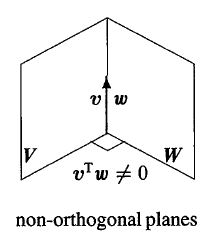
\includegraphics{week5/orthogonality}
\caption{Orthogonality is impossible when $\dim\bm U+\dim\bm V>\dim(\bm U\cup\bm V)$}
\end{figure}
\end{example}
\begin{remark}
When a vector is in two orthogonal subspaces, it \textit{must} be zero. It is \emph{perpendicular} to
itself. 
\\The reason is clear: this vector $\bm u\in\bm U$ and $\bm u\in\bm V$, so $\inp{\bm u}{\bm u}=0$. It has to be zero vector.
\end{remark}
If two subspaces are perpendicular, their basis must be ind.
\begin{theorem}
Assume $\{u_1,\dots,u_k\}$ is the basis for $\bm U$, $\{v_1,\dots,v_l\}$ is the basis for $\bm V.$ If $\bm U\perp\bm V$ ($u_i\perp v_j$ for $\forall i,j$), then $u_1,u_2,\dots,u_k,v_1,v_2,\dots,v_l$ must be ind.
\end{theorem}
\begin{proof}
Suppose there exists $\{\alpha_1,\dots,\alpha_k\}$ and $\{\beta_1,\dots,\beta_l\}$ such that
\[
\alpha_1u_1+\dots+\alpha_ku_k+\beta_1v_1+\dots+\beta_lv_l=\bm 0
\]
then equivalently,
\[
\alpha_1u_1+\dots+\alpha_ku_k=-(\beta_1v_1+\dots+\beta_lv_l).
\]
Then we set $\bm w=\alpha_1u_1+\dots+\alpha_ku_k$, obviously, $\bm w\in\bm U$ and $\bm w\in\bm V$.

 Hence it must be zero (This is due to remark above). Thus we have
\begin{gather*}
\alpha_1u_1+\dots+\alpha_ku_k=\bm 0\\
\beta_1v_1+\dots+\beta_lv_l=\bm 0.
\end{gather*}
Due to the independence, we have $\alpha_i=0$ and $\beta_j=0$ for $\forall i,j$. 
\end{proof}
\begin{corollary}
For subspaces $\bm U$ and $\bm V$, we obtain
\[
\dim(\bm U\cup\bm V)\le \dim(\bm U) + \dim(\bm V).
\]
\end{corollary}
For subspaces $\bm U$ and $\bm V\in\mathbb{R}^{n}$, if $\mathbb{R}^{n}=\bm U\cup\bm V$, and moreover, $n=\dim(\bm U)+\dim(\bm V)$, then we say $\bm V$ is the \emph{orthogonal complement} of $\bm U$.
\begin{definition}[orthogonal complement]
For subspaces $\bm U$ and $\bm V\in\mathbb{R}^{n}$, if $\dim(\bm U)+\dim(\bm V)=n$ and $\bm U\perp\bm V$, then we say $\bm V$ is the \emph{orthogonal complement} of $\bm U$. We denote $\bm V$ as $\bm U^{\perp}$.

Moreover, $\bm V=\bm U^{\perp}$ iff $\bm V^{\perp}=\bm U$.
\end{definition}
\begin{example}
Suppose $\bm U\cup\bm V=\mathbb{R}^{3}$, $\bm U=\Span\{\bm e_1,\bm e_2\}$. If $\bm V$ is the orthogonal complement of $\bm U$, then $\bm V=\Span\{\bm e_3\}$.
\end{example}

Next we study the relationship between the null space and the row space in $\mathbb{R}^n$.
\begin{theorem}[Fundamental theorem for linear alegbra, part 2] Given $\bm A\in\mathbb{R}^{m\times n}$,

\emph{$N(\bm A)$ is the orthogonal complement of the row space of $\bm A$, $\mathcal{C}(\bm A\trans)$ (in $\mathbb{R}^{n}$).}

\emph{$N(\bm A\trans)$ is the orthogonal complement of the column space $\mathcal{C}(\bm A)$ (in $\mathbb{R}^{m}$).}
\end{theorem}
\begin{proof}
\begin{itemize}
\item
Firstly, we show $\dim(N(\bm A))+\dim(\mathcal{C}(\bm A\trans))=n$:

We know that $\dim(N(\bm A))=n-r$ and $\dim(\mathcal{C}(\bm A\trans)) = r$, where $r=\rank(\bm A)$.

Hence $\dim(N(\bm A))+\dim(\mathcal{C}(\bm A\trans))=n$.
\item
Then we show $N(\bm A)\perp \mathcal{C}(\bm A\trans)$:

For any $x\in N(\bm A)$, if we set $\bm A=\begin{bmatrix}
a_1\trans\\a_2\trans\\\vdots\\a_m\trans
\end{bmatrix}$, then we obtain:
\[
\bm{Ax}=\begin{bmatrix}
a_1\trans\\a_2\trans\\\vdots\\a_m\trans
\end{bmatrix}\begin{bmatrix}
\bm x
\end{bmatrix}=\begin{bmatrix}
0\\0\\\vdots\\0
\end{bmatrix}
\]
Hence \textit{every row has a zero product with} $\bm x$, i.e., $\inp{a_i}{\bm x}=0$ for $\forall i\in\{1,2,\dots,m\}$.

For any $y=\sum_{i=1}^m\alpha_ia_i\in \mathcal{C}	(\bm A\trans)$, we obtain:
\[
\begin{aligned}
\inp{\bm x}{y}&=\inp{y}{\bm x}=\inp{\sum_{i=1}^m\alpha_ia_i}{\bm x}\\
&=\sum_{i=1}^{m}\alpha_i\inp{a_i}{\bm x}=0.
\end{aligned}
\]
Hence $\bm x\perp y$ for $\forall \bm x\in N(\bm A)$ and $y\in \mathcal{C}(\bm A\trans)$.\\
\end{itemize}
Hence $N(\bm A)^{\perp}=\mathcal{C}(\bm A\trans)$. Similarly, we have $N(\bm A\trans)^{\perp}=\mathcal{C}(\bm A)$. 
\end{proof}

\begin{corollary}
$\bm{Ax}=\bm b$ is solvable if and only if $\bm y\trans\bm A=\bm 0$ implies $\bm y\trans\bm b$=0.
\end{corollary}
\begin{proof} The following statements are equivalent:
\begin{itemize}
\item
$\bm{Ax}=\bm b$ is solvable.
\item
$\bm b\in \mathcal{C}(\bm A)$.
\item
$\bm b\in N(\bm A\trans)^{\perp}$
\item
$\bm y\trans\bm b=0$ for $\forall y\in N(\bm A\trans)$
\item
Given $\bm y\trans\bm A=\bm 0$, i.e., $y\in N(\bm A\trans)$, it implies $\bm y\trans\bm b=0$.
\end{itemize}
\end{proof}
The \emph{Inverse Negative Proposition} is more commonly useful:
\begin{corollary}
$\bm{Ax}=\bm b$ has no solution if and  and only if $\exists \bm y$ s.t. $\bm y\trans\bm A=0$ and $\bm y\trans\bm b\ne 0$.
\end{corollary}
We could extend this corollary into general case:
\begin{remark}
\begin{theorem}\label{theorem_12.3}
$\bm{Ax}\ge\bm b$ has no solution if and only if $\exists \bm y\ge\bm 0$ such that $\bm y\trans\bm A=\bm 0$ and $\bm y\trans\bm b\ge \bm 0$.
\end{theorem}
$\bm y\trans\bm A=0$ requires that there exists one linear combination of the row space to be zero.

The complete proof for this theorem is not required in this course. We only show the necessity case.
\begin{proof}[Necessity case.]
Suppose $\exists \bm y\ge\bm 0$ such that $\bm y\trans\bm A=\bm 0$ and $\bm y\trans\bm b\ge \bm 0$. Assume there exists $x^{*}$ such that $\bm Ax^{*}\ge\bm b$. By postmultiplying $\bm y\trans$ we have 
\[\bm y\trans\bm Ax^{*}\ge\bm y\trans\bm b>\bm 0
\implies 
\bm 0>\bm 0.
\]
which is a contradiction!
\end{proof}
\end{remark}

\begin{example}
Given the system 
\begin{align}
x_1+x_2&\ge1\label{Eq:6:3}
\\
-x_1&\ge-1\label{Eq:6:4}
\\
-x_2&\ge2\label{Eq:6:5}
\end{align}
Eq.(\ref{Eq:6:3})$\x$1+Eq(\ref{Eq:6:4})$\x$1+Eq.(\ref{Eq:6:5})$\x$1 gives
\[
0\ge 2
\]
which is a contradiction!\\
So the key idea of theorem (\ref{theorem_12.3}) is to construct a linear combination of row space to let it become zero. If the right hand is larger than zero, then this system has no solution.
\end{example}
\begin{remark}
\begin{corollary}
If $\bm A=\bm A\trans$, then $N(\bm A\trans)^{\perp}=\mathcal{C}(A)=\mathcal{C}(\bm A\trans)=N(\bm A)$.
\end{corollary}
\begin{corollary}\label{corollary_12.5}
The system $\bm{Ax}=\bm b$ may not have a solution, but $\bm A\trans\bm A\bm x=\bm A\trans\bm b$ always have at least one solution for $\forall\bm b$.
\end{corollary}
\begin{proof}
Since $\bm A\trans\bm A$ is symmetric, we have $\mathcal{C}(\bm A\trans\bm A)=\mathcal{C}(\bm A\bm A\trans)$. Show by yourself that $\mathcal{C}(\bm A\bm A\trans)=\mathcal{C}(\bm A\trans)$, hence $\mathcal{C}(\bm A\trans\bm A)=\mathcal{C}(\bm A\trans)$.

For any vector $\bm b$, we have $\bm A\trans\bm b\in \mathcal{C}(\bm A\trans)\implies\bm A\trans\bm b\in \mathcal{C}(\bm A\trans\bm A)$, which means there exists a linear combination of the columns of $\bm A\trans\bm A$ that equals to $\bm b$.

Or equivalently, there exists a solution to $\bm A\trans\bm A\bm x=\bm A\trans\bm b$.
\end{proof}
\begin{corollary}\label{corollary_12.6}
$\bm A\trans\bm A$ is invertible if and only if $\bm A$ is full column rank, i.e., columns of $\bm A$ are ind.
\end{corollary}
\begin{proof}
We have shown that $C(\bm A\trans\bm A)=C(\bm A\trans)$.

Hence $C(\bm A\trans\bm A)^{\perp}=C(\bm A\trans)^{\perp}\implies N(\bm A\trans\bm A)=N(\bm A)$.

Thus, the following statements are equivalent:
\begin{itemize}
\item
$\bm A$ has ind. columns
\item
$N(\bm A)=\{\bm 0\}$
\item
$N(\bm A\trans\bm A)=\{\bm 0\}$
\item
$\bm A\trans\bm A$ is invertible.
\end{itemize}
\end{proof}
\end{remark}
\subsection{Least Squares Approximations}
The linear system $\bm{Ax}=\bm b$ often has no solution, if so, what should we do?

We cannot always get the error $\bm e=\bm b-\bm{Ax}$ down to zero, so we want to use \textit{least square method} to minimize the error. In other words, our goal is to
\[
\min_{\bm x\in\mathbb{R}^n}\bm e^2:=\min_{\bm x}\|\bm{Ax}-\bm b\|^2=\sum_{i=1}^{m}(a_i\trans\bm x-b_i)^2
\]
where $\bm A\in\mathbb{R}^{m\times n}$ and $\bm b\in\mathbb{R}^m$. The minimizer $\bm x$ is called the \emph{linear least squares solution}.

\subsubsection{Least Squares by Convex Optimization}
Firstly, you should know some basic calculus knowledge for matrix:
\paragraph{The Chian Rule} Given two vectors $f(x),g(x)$ of appropriate size,
\[
\frac{\partial(f\trans g)}{\partial x}=\frac{\partial f(x)}{\partial x}g(x)+\frac{\partial g(x)}{\partial x}f(x)
\]
\paragraph{Examples of Matrix Derivative}
\begin{align}
\frac{\partial(a\trans \bm x)}{\partial \bm x}&=a\\
\frac{\partial(a\trans \bm A\bm x)}{\partial \bm x}&=\frac{\partial((\bm A\trans a)\trans\bm x)}{\partial \bm x}=\bm A\trans a\\
\frac{\partial(\bm A\bm x)}{\partial \bm x}&=\bm A\trans\\
\frac{\partial(\bm x\trans\bm A\bm x)}{\partial \bm x}&=\bm A\bm x+\bm A\trans\bm x
\end{align}

Thus, in order to minimize $\|\bm{Ax}-\bm b\|^2=(\bm{Ax}-\bm b)\trans(\bm{Ax}-\bm b)$, it suffices to let its \emph{derivative} with respect to $\bm x$ to be \emph{zero.} (Since $\|\bm{Ax}-\bm b\|^2$ is convex, which will be discussed in detail in other courses.) Hence we have:
\[\begin{aligned}
\frac{\partial (\bm{Ax}-\bm b)\trans(\bm{Ax}-\bm b)}{\partial \bm x}&=\frac{\partial(\bm{Ax}-\bm b)}{\partial \bm x}(\bm{Ax}-\bm b)+\frac{\partial(\bm{Ax}-\bm b)}{\partial \bm x}(\bm{Ax}-\bm b)\\
&=2\frac{\partial(\bm{Ax}-\bm b)}{\partial \bm x}(\bm{Ax}-\bm b)\\
&=2(\frac{\partial(\bm A\bm x)}{\partial \bm x}-\frac{\partial(\bm b)}{\partial \bm x})(\bm{Ax}-\bm b)\\
&=2\bm A\trans(\bm{Ax}-\bm b)=\bm 0.
\end{aligned}
\]
Or equivalently, 
\[
\bm A\trans\bm{Ax}=\bm A\trans\bm b.
\]
According to corollary (\ref{corollary_12.5}), this equation always exists a solution. This equation is called the \emph{normal equation}.
\begin{theorem}\label{theorem_12.4}
A vector $\bm x_{\text{LS}}$ is an optimal solution to the least squares problem
\begin{subequations}
\begin{equation}
\min_{\bm x\in\mathbb{R}^n}\|\bm b-\bm{Ax}\|_2^2
\end{equation}
if and only if it satisfies
\begin{equation}
\bm A\trans\bm A\bm x_{\text{LS}} = \bm A\trans\bm b.
\end{equation}
\end{subequations}
\end{theorem}
\subsubsection{Fit a stright line}
Given a collection of data $(\bm x_i,y_i)$ for $i=1,\dots,m$, we can use a stright line to fit these points:
\[
\left\{
\begin{aligned}
y_1&=a_0+a_1x_{1,1}+a_2x_{1,2}+\dots+a_nx_{1,n}+\varepsilon_1\\
y_2&=a_0+a_1x_{2,1}+a_2x_{2,2}+\dots+a_nx_{2,n}+\varepsilon_2\\
\vdots\\
y_m&=a_0+a_1x_{m,1}+a_2x_{m,2}+\dots+a_nx_{m,n}+\varepsilon_m
\end{aligned}
\right.
\]
Our fit line is 
\[
\hat y=a_0+a_1x_1+a_2x_2+\dots+a_nx_n
\]
In \textit{compact matrix form}, we have
\[
\begin{bmatrix}
y_1\\y_2\\\vdots\\y_n
\end{bmatrix}
=\begin{bmatrix}
1&x_{1,1}&x_{1,2}&\dots&x_{1,n}\\
1&x_{2,1}&x_{2,2}&\dots&x_{2,n}\\
\vdots&\vdots&&&\\
1&x_{m,1}&x_{m,2}&\dots&x_{m,n}\\
\end{bmatrix}\begin{bmatrix}
a_0\\a_1\\a_2\\\vdots\\a_{n}
\end{bmatrix}+\begin{bmatrix}
\varepsilon_1\\\varepsilon_2\\\vdots\\\varepsilon_m
\end{bmatrix}
\]
Or equivalently, we have 
\[
\bm y=\bm{Ax}+\bm \varepsilon
\]
where $\bm A =\begin{bmatrix}
1&x_{1,1}&x_{1,2}&\dots&x_{1,n}\\
1&x_{2,1}&x_{2,2}&\dots&x_{2,n}\\
\vdots&\vdots&&&\\
1&x_{m,1}&x_{m,2}&\dots&x_{m,n}\\
\end{bmatrix}_{m\times (n+1)}$, $\bm x=\begin{bmatrix}
a_0\\a_1\\a_2\\\vdots\\a_{n}
\end{bmatrix}_{(n+1)\times 1}$, $\bm \varepsilon=\begin{bmatrix}
\varepsilon_1\\\varepsilon_2\\\vdots\\\varepsilon_m
\end{bmatrix}_{m\times 1}$.\\
Our goal is to minimize $\|\hat{\bm y}-\bm y\|^2=\|\bm{Ax}-\bm y\|^2$. Then by theorem (\ref{theorem_12.4}), it suffices to sovle $\bm A\trans\bm A\bm x=\bm A\trans\bm y$.

\subsection{Projections}
In corollary (\ref{corollary_12.6}), we know that if $\bm A$ has ind. columns, then $\bm A\trans\bm A$ is invertible. On this condition, the normal equation $\bm A\trans\bm A\bm x=\bm A\trans\bm b$ has the unique solution $\bm x^{*}=(\bm A\trans\bm A)^{-1}\bm A\trans\bm b$, which follows that the error $\bm b-\bm A\bm x^{*}$ is minimized. Note that $\bm A\bm x^{*}=\bm A(\bm A\trans\bm A)^{-1}\bm A\trans\bm b$ is \emph{approximately} equal to $\bm b$. 
\begin{itemize}
\item
If $\bm b$ and $\bm{A}\bm x^{*}$ are exactly in the same space, i.e., $\bm b\in\mathcal{C}(\bm A)$, then $\bm{A}\bm x^{*}=\bm b$. The error is equal to zero.
\item
Otherwise, just as the Figure (\ref{figure_12.2}) shown, $\bm A\bm x^{*}$ is the projection of $\bm b$ to subspace $\mathcal{C}(\bm A)$.
\end{itemize}
\begin{figure}[t]
\centering
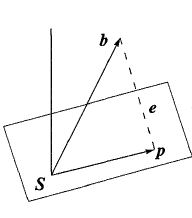
\includegraphics{week5/projection}
\caption{The projection of $\bm b$ onto a subspace $\bm S:=\mathcal{C}(\bm A)$.}\label{figure_12.2}
\end{figure}
\begin{definition}[Projection]
Let $\bm S\in\mathbb{R}^{m}$ be a non-empty closed set and $\bm b\in\mathbb{R}^m$ be given. Then the projection of $\bm b$ onto the set $\bm S$ is the solution to
\[
\min_{\bm z\in\bm S}\|\bm z-\bm b\|_2^2,
\]
where we use notation $\Proj_{\bm S}(\bm b)$ to denote the projection of $\bm b$ onto $\bm S$.
\end{definition}
By definition, the projection of $\bm b$ onto the subspace $\mathcal{C}(\bm A)$ is given by 
\[
\Proj_{\mathcal{C}(\bm A)}(\bm b):=\bm A\bm x^*,\quad
\text{where }\bm x^*=\arg\min_{\bm x\in\mathbb{R}^n}\|\bm{Ax} - \bm b\|.
\]

\begin{definition}[Projection matrix]
Given the projection
\[
\Proj_{C(\bm A)}(\bm b):=\bm A\bm x^{*}=\bm A(\bm A\trans\bm A)^{-1}\bm A\trans\bm b,
\]
since $[\bm A(\bm A\trans\bm A)^{-1}\bm A\trans]\bm b$,
we call the projection operator $\bm P:=\bm A(\bm A\trans\bm A)^{-1}\bm A\trans$ as the \emph{projection matrix} of $\bm A$.
\end{definition}
\begin{definition}[Idempotent]
Let $\bm A$ be a \emph{square} matrix that satisfies $\bm A=\bm A\bm A$, then $\bm A$ is called an \emph{idempotent} matrix.
\end{definition}
Let's show that the projection matrix is \textit{idempotent}:
\[
\begin{aligned}
\bm P^{2}&=\bm A(\bm A\trans\bm A)^{-1}\bm A\trans\bm A(\bm A\trans\bm A)^{-1}\bm A\trans\\
&=\bm A(\bm A\trans\bm A)^{-1}(\bm A\trans\bm A)(\bm A\trans\bm A)^{-1}\bm A\trans\\
&=\bm A(\bm A\trans\bm A)^{-1}\bm A\trans=\bm P.
\end{aligned}
\]

\subsubsection{Observations}
\begin{itemize}
\item
Suppose $\bm b\in \mathcal{C}(\bm A)$, i.e., $\exists \bm x$ s.t. $\bm{Ax}=\bm b$. Then the projection of $\bm b$ is exactly $\bm b$:
\[
\begin{aligned}
\bm{Pb}&=\bm A(\bm A\trans\bm A)^{-1}\bm A\trans(\bm b)\\
&=\bm A(\bm A\trans\bm A)^{-1}\bm A\trans(\bm{Ax})\\
&=\bm A(\bm A\trans\bm A)^{-1}(\bm A\trans\bm A)\bm x\\
&=\bm{Ax}=\bm b.
\end{aligned}
\]
\item
Assume $\bm A$ has only one column, say, $\bm a$. Then we have
\[\begin{aligned}
\bm x^{*}&=(\bm A\trans\bm A)^{-1}\bm A\trans\bm b=\frac{\bm a\trans\bm b}{\bm a\trans\bm a}\\
\bm A\bm x^{*}&=\bm{Pb}=\bm A(\bm A\trans\bm A)^{-1}\bm A\trans(\bm b)=\frac{\bm a\trans\bm b}{\bm a\trans\bm a}\times\bm a=\frac{\bm a\trans\bm b}{\|\bm a\|^2}\times\bm a
\end{aligned}
\]
More interestingly, 
\[\frac{\bm a\trans\bm b}{\|\bm a\|^2}\times\bm a=\frac{\|\bm a\|\|\bm b\|\cos\theta}{\|\bm a\|^2}\times\bm a=\|\bm b\|\cos\theta\times\frac{\bm a}{\|\bm a\|}\]
which is the projection of $\bm b$ onto a line $\Span\{\bm a\}$. (Shown in figure (\ref{Fig:6:3}).)
\begin{figure}[H]
\centering
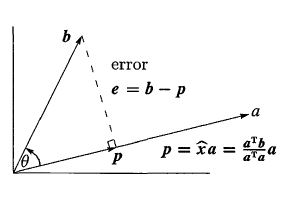
\includegraphics[width=10cm]{week5/projection_line}
\caption{The projection of $\bm b$ onto a line $\bm a$.}
\label{Fig:6:3}
\end{figure}
More generally, we can write the projection of $\bm b$ onto the line $\Span\{\bm a\}$ as:
\[
\Proj_{\Span\{\bm a\}}(\bm b)=\frac{\inp{\bm a}{\bm b}}{\inp{\bm a}{\bm a}}\bm a
\]
\paragraph{Changing an Orthogonal Basis}
Note that the error $\bm b-\Proj_{\Span\{\bm a\}}(\bm b)$ is perpendicular to $\bm a$, and $\bm b-\Proj_{\Span\{\bm a\}}(\bm b)\in\Span\{\bm a,\bm b\}.$

If we define $\bm b'=\bm b-\Proj_{\Span\{\bm a\}}(\bm b)$, then it's easy to check that $\Span\{\bm a,\bm b'\}=\Span\{\bm a,\bm b\}$ and $\bm a\perp\bm b'$. 

Hence, we convert the basis $\{\bm a,\bm b\}$ into another basis $\{\bm a,\bm b'\}$ such that the elements are orthogonal to each other. For general subspace we could also use this approach to obtain an orthogonal basis, which will be discussed in next lecture. 
\end{itemize}









%\section{Assignment Eight}\index{Assignment_Eight}
\begin{enumerate}
\item
Let $\bm A$ be an $n\x n$ matrix. Show that $\bm A\trans\bm A$ and $\bm A\bm A\trans$ are \textit{similar}.
\item
Let $\bm A$ be $m\times n$ ($m\ge n$) matrix with singular value decomposition $\bm U\Sigma\bm V\trans$. Let $\Sigma^+$ denote the $n\times m$ matrix
\[
\begin{pmatrix}
\frac{1}{\sigma_1}&&&0&\dots&0\\
&\ddots&&\vdots&\ddots&\vdots\\
&&\frac{1}{\sigma_n}&0&\dots&0\\
\end{pmatrix}
\]
And we define $\bm A^+=\bm V\Sigma^+\bm U\trans$
\begin{enumerate}
\item
Show that
\[
\bm A\bm A^+=\begin{bmatrix}
\bm I_n&\bm0\\\bm0&\bm0
\end{bmatrix}\qquad\text{and}\qquad
\bm A^+\bm A=\bm I_n.
\]
(Note that $\bm A^+$ is called the \emph{pseudo-inverse} of $\bm A$.)
\item
If $\rank(\bm A)=n$, Show that $\hat{\bm x}=\bm A^+\bm b$ satisfies the normal equation $\bm A\trans\bm A\bm x=\bm A\trans\bm b.$
\end{enumerate}
\item
Suppose $\bm A\in\mathbb{R}^{m\x n}(m\ge n)$ has an SVD 
\[
\bm A=\sigma_1\bm u_1\bm v_1\trans+\dots+\sigma_n\bm u_n\bm v_n\trans
\]
where $\sigma_1\ge\sigma_2\ge\dots\ge\sigma_n\ge0.$
\begin{enumerate}
\item
Prove that $\|\bm A\|_{F}^2=\sum_{i=1}^{n}\sigma_i^2$.
\item
Let $\bm A_k$ be the \textit{best rank-k approximation} of $\bm A$, what is $\|\bm A-\bm A_k\|_{F}$?
\end{enumerate}
\item
Suppose the \textit{maximal singular value} of $\bm A\in\mathbb{R}^{m\x n}$ is $\sigma_1$, prove 
\[
\sigma_1=\max_{\bm x,\bm y}\bm x\trans\bm A\bm y
\]
where $\bm x\in\mathbb{R}^m,\bm y\in\mathbb{R}^n,\|\bm x\|=\|\bm y\|=1.$
\item
Let $\bm A$ be a \textit{symmetric positive definite} $n\x n$ matrix. Show that $\bm A$ can be factored into a product $\bm Q\bm Q\trans$, where $\bm Q$ is an $n\x n$ matrix whose columns are \textit{mutually orthogonal.}
\end{enumerate}
%
\chapter{Midterm}

\section{Sample Exam}\index{Sample Exam}
DURATION OF EXAMINATION: 2 hours in-class\\
\textit{This examination paper includes $6$ pages and $6$ problems. You are responsible for ensuring that
your copy of the paper is complete. Bring any discrepancy to the attention of your invigilator.}\\
\begin{enumerate}
\item \textbf{(30 points)} \textit{Solving a linear system of equations}\\
For a real number $c$, consider the linear system:
\begin{align}
x_1+x_2+cx_3+x_4&=c\\
-x_2+x_3+2x_4&=0\\
x_1+2x_2+x_3-x_4&=-c
\end{align}
do the following:
\begin{enumerate}
\item
Write out the \textit{coefficient matrix} of the system.\\
\item
Write out the \textit{augmented matrix} for this system and calculate its \textit{row-reduced echelon form.}\\
\item
Write out the complete set of solutions in \textit{vector form.}\\
\item
What is the \textit{rank} of the coefficient matrix $\bm A$? Justify your answer.\\
\item
Find a \textit{basis}  of the subspace of solutions when $c=0$.
\end{enumerate}
\newpage
\item \textbf{(20 points)} \textit{Vector space}\\
Find a \textit{basis} for each of the following spaces.
\begin{itemize}
\item
Space of $n\x n$ \textit{skew symmetric matrices} (i.e. those matrix satisfying $\bm A=-\bm A\trans$)\\
\item
The space of all \textit{polynomials} of the form $ax^2+bx+2a+3b$, where $a,b\in\mathbb{R}.$\\
\item
$\Span\{x-1,x+1,2x^2-2\}.$
\end{itemize}
\newpage
\item \textbf{(15 points)} \textit{Matrix multiplications}\\
Prove the following statements:
\begin{enumerate}
\item
Define the set of $n\x n$ \textit{diagonol matrices} to be $\kappa$. Prove that for a diagonal matrix $\bm D$ with \textit{distinct} elements (i.e. $\bm D_{ii}\ne\bm D_{jj},\forall i\ne j$), the set $\{\bm A\in\mathbb{R}^{n\x n}|\bm{AD}=\bm{DA}\}$ is exactly $\kappa$.\\
\item
If an $n\x n$ matrix $\bm A$ satisfies $\bm{AB}=\bm{BA}$ for any $n\x n$ matrix $\bm B$, then $\bm A$ must be of the form $c\bm I$, where $c$ is a scalar.
\end{enumerate}
\newpage
\item \textbf{(10 points)} \textit{Matrix Inverse}\\
\begin{enumerate}
\item
Compute the inverse of the matrix $\begin{pmatrix}
5&4\\4&5
\end{pmatrix}.$
\item
Compute the inverse of the matrix $\begin{pmatrix}
a&b\\c&d
\end{pmatrix}$ if exists. When does the inverse of the matrix exist?
\end{enumerate}
\newpage
\item \textbf{(15 points)} \textit{Matrix rank}\\
\begin{enumerate}
\item
Suppose $\bm u\in\mathbb{R}^{n\x 1}$ satisfies $\|\bm u\|=1$. What is the rank of the matrix $\bm I-\bm u\bm u\trans$?\\
\item
Suppose $\bm u\in\mathbb{R}^{n\x 1}$ satisfies $\|\bm u\|=1$. Define $\bm P=\bm I-\bm u\bm u\trans$. What is the rank of $\bm P^2$? What about $\bm P^5$?\\
\item
Suppose $\bm x,\bm y\in\mathbb{R}^{n\x 1}$. What is the rank of the matrix $\bm I-\bm x\bm y\trans$?\end{enumerate}
\newpage
\item \textbf{(20 points)} \\
State your answers. No justifications are required.
\begin{enumerate}
\item
We know $a^2-b^2=(a+b)(a-b)$, where $a,b\in\mathbb{R}$. When $\bm A,\bm B$ are square matrices, can we
represent $\bm A^2-\bm B^2$ by only $(\bm A+\bm B)(\bm A-\bm B)$?\\
\item
True or False: If $\bm A$ and $\bm B$ are \textit{invertible}, then $\bm A+\bm B$ is also \textit{invertible}.\\
\item
True or False: The set of all \textit{real-valued} functions on $\mathbb{R}$ such that $f(1)=0$ is a \textit{vector space}.\\
\item
True or False: The product of two \textit{invertible} $n\x n$ matrices is \textit{invertible}\\
\item
True or False: If two matrices have the same \textit{reduced row echelon form}, then they have the
same \textit{column space}.\\
\item
True or False: If two columns of the square $\bm A$ are the same, then $\bm A$ \textit{cannot} be invertible.\\
\item
True or False: For an $m\x n$ matrice $\bm A$, $\rank(\bm A)+\dim(\row(\bm A))=n.$
\end{enumerate}
\end{enumerate}
%\section{Final Exam}\index{Sample Exam}
DURATION OF EXAMINATION: 2 hours and 35 minutes in-class\\
\textit{This examination paper includes $6$ pages and $6$ problems. You are responsible for ensuring that
your copy of the paper is complete. Bring any discrepancy to the attention of your invigilator.}\\
\begin{enumerate}
\item \textbf{(20 points)} \textit{Matrix representation for linear transformation}\\
\begin{enumerate}
\item
Let $T$ be the transformation
\begin{gather*}
T:\{\textbf{polynomials of degree $\le4$}\}\mapsto\{\textbf{polynomials of degree $\le4$}\}\\
\qquad\qquad\qquad\qquad\qquad T(p)=(x-2)\frac{\diff p}{\diff x}
\end{gather*}
Show that $T$ is a \textit{linear transformation} and write down a \textit{matrix representation} of $T$ with respect to basis $\{1,x,x^2,x^3,x^4\}$ for the input and output space.\\
\item
If a polynomial $f(x)$ satisfies
\[
T(f)=\lambda f,
\]
we say $f$ is an \textit{eigenvector} of $T$. Find two \textit{linearly independent} eigenvectors of $T$.
\end{enumerate}
\newpage
\item \textbf{(20 points)} \textit{Least Square Method}\\
\begin{enumerate}
\item
Find the projection of $\bm z=\begin{bmatrix}
1\\0\\1
\end{bmatrix}$ onto the column space of $\begin{bmatrix}
1&-1\\1&-1\\-2&4
\end{bmatrix}.$\\
\item
Let $\mathcal{A}:\mathbb{R}^{2\x 1}\mapsto\mathbb{R}^{2\x 2}$ be a mapping defined as
\[
\mathcal{A}\begin{bmatrix}
a\\b
\end{bmatrix}=\begin{bmatrix}
a+b&a-b\\-2a+4b&0
\end{bmatrix},\forall a,b\in\mathbb{R}.
\]
Define $\kappa=\{\bm{Ax}|\bm x\in\mathbb{R}^{2\x 1}\}$.\\
Find the best approximation of $\bm B=\begin{bmatrix}
1&2\\7&1
\end{bmatrix}$ in the space $\kappa$.\\
\textit{Hint: Consider $\begin{bmatrix}
1&2\\7&1
\end{bmatrix}$ and $\begin{bmatrix}
a+b&a-b\\-2a+4b&0
\end{bmatrix}$ as $\mathbb{R}^{4\x 1}$ vector.\\
Then you only need to find the best approximation of $\begin{pmatrix}
1\\2\\7\\1
\end{pmatrix}$ onto the set $\{\bm{Ax}|\bm x\in\mathbb{R}^{2\x 1}\}$, where $\bm A=\begin{bmatrix}
1&1\\1&-1\\-2&4\\0&0
\end{bmatrix}.$}
\end{enumerate}
\newpage
\item \textbf{(20 points)} \\
True or False. No justifications are required.
\begin{enumerate}
\item
If all the entries of a square matrix $\bm A$ are \textit{positive}, then $\bm A^{-1}$ exist.\\
\item
If $\bm Q$ is an \textit{orthogonal matrix}, then $\det(\bm Q)=\pm1$.\\
\item
If $\bm A$ is a \textit{negative definite} matrix, then its singular values have the same absolute values as its eigenvalues.\\
\textit{Hint: Note that $\bm A$ is said to be negative definite when $-\bm A$ is positive definite.}\\
\item
If $\bm A$ is an $n\x n$ matrix with \textit{characteristic polynomial} $p_{\bm A}(t)=t^n$, then $\bm A=\bm 0.$\\
\item
If $\bm A$ is the sum of 5 rank one matrices, then $\rank(\bm A)\le5.$
\end{enumerate}
\newpage
\item \textbf{(20 points)} \textit{SVD decomposition} \\
The question is about the matrix
\[
\bm A=\begin{bmatrix}
0&-1\\4&0
\end{bmatrix}
\]
\begin{enumerate}
\item
Find its eigenvalues and eigenvectors, write the vector $\bm u=\begin{bmatrix}
2\\0
\end{bmatrix}$ as a combination of those eigenvectors.\\
\item
Do the SVD decomposition to derive $\bm A=\bm U\Sigma\bm V\trans$ in two steps:
\begin{itemize}
\item
First, compute $\bm V$ and $\Sigma$ using the matrix $\bm A\trans\bm A$.
\item
Second, find the (\textit{orthonormal}) columns of $\bm U$.
\end{itemize}
\end{enumerate}
\newpage
\item \textbf{(15+5 points)} \textit{Eigenvalues and Eigenvectors}\\
\begin{enumerate}
\item
Suppose $\bm A,\bm B\in\mathbb{R}^{n\x n}$ can can be \textit{diagonalized} by the same matrix, prove that $\bm{AB}=\bm{BA}.$\\
\textit{Hint: Note that $\bm A$ is said to be diagonalized by $\bm S$ if $\bm S^{-1}\bm A\bm S$ is diagonal.}\\
\item
Suppose $\bm A,\bm B\in\mathbb{R}^{n\x n}$ satisfy $\bm{AB}=\bm{BA}$, and both $\bm A$ and $\bm B$ are diagonalizable. $\bm A$ has $n$ \textit{distinct} eigenvalues. Prove that $\bm A,\bm B$ can can be \textit{diagonalized} by the same matrix.\\
\textit{Hint: Suppose $\bm A$ has eigenvectors $\bm v_1,\dots,\bm v_n$. You can express $\bm B\bm v_i$ as linear combination of $\bm v_1,\dots,\bm v_n$. Then you can express $\bm A(\bm B\bm v_i)$ and $\bm B(\bm A\bm v_i)$. Finally compute $\bm A(\bm B\bm v_i)-\bm B(\bm A\bm v_i)$ to derive something.}\\
\item \textbf{(bonus question)}\\
Prove part $(b)$ without the assumption that $\bm A$ has $n$ \textit{distinct} eigenvalues. (i.e. $\bm A$ might have \emph{repeated} eigenvalues)\\
\textit{Hint: Since $\bm A$ is diagonalizable, there exists $\bm Q$ such that $\bm Q^{-1}\bm A\bm Q=\bm D$, where $\bm D$ is diagonal. Then you should express $\bm D$. Then you compute $\bm Q^{-1}\bm B\bm Q=\bm C$, i.e. partition $\bm C$ in the same way of $\bm D$. Next you should show us that $\bm C$ is block diagonal. Then you construct \emph{diagonal} matrix $\bm T_*$ that diagonalize $\bm C$. Finally you construct $\bm P$ that diagonalize both $\bm A$ and $\bm B$.}
\end{enumerate}
\newpage
\item \textbf{(10 points)} \textit{Positive definite}\\
Suppose $\bm A,\bm B\in\mathbb{R}^{n\x n}$, where $\bm A=\begin{bmatrix}
a_{ij}
\end{bmatrix}_{i,j=1}^{n}, \bm B=\begin{bmatrix}
b_{ij}
\end{bmatrix}_{i,j=1}^{n}$.\\
Define the \emph{Hadamard product} $\bm A\circ\bm B$ as an $n\x n$ matrix with entries
\[
\begin{bmatrix}
\bm A\circ\bm B
\end{bmatrix}_{ij}=a_{ij}b_{ij}.
\]
For example, if $\bm A=\begin{bmatrix}
1&2\\3&7
\end{bmatrix},\bm B=\begin{bmatrix}
0&\pi\\1&e
\end{bmatrix},$ then $\bm A\circ\bm B=\begin{bmatrix}
0&2\pi\\3&7e
\end{bmatrix}.$\\
Prove the following statements:
\begin{enumerate}
\item
$\rank(\bm A\circ\bm B)\le\rank(\bm A)\rank(\bm B)$;
\\
\textit{Hint: Extend Hadamard product into vector. Then it's easy to verify that $(\bm A\circ\bm B)\circ\bm C=\bm A\circ\bm C+\bm B\circ\bm C$ and $(\bm u_1\bm v_1\trans)\circ(\bm u_2\circ\bm v_2\trans)=(\bm u_1\circ\bm u_2)\x(\bm v_1\circ\bm v_2)\trans$. Then you can do SVD decomposition for $\bm A$ and $\bm B$ (vector form, related to rank.) Then you can express $\bm A\circ\bm B$ as the sum of some matrices with rank 1.}
\\
\item
If $\bm A\succeq0,\bm B\succeq0$ and $\bm A,\bm B$ are \textit{symmetric matrix}, prove that
\[
\bm A\circ\bm B\succeq0.
\]
\textit{Hint: Note that $\bm A=\bm R\trans\bm R$, where $\bm R$ is square. Then you should express $\bm R\trans\bm R$ into vector form. Similarly, you can express $\bm B$ into vector form. Then you compute $\bm A\circ\bm B$ and show it is PSD by definition.}
\end{enumerate}
\end{enumerate}

%
\chapter{Solution}

\section{Assignment Solutions}\index{Assignment Solution}
\subsection{Solution to Assignment One}
\begin{enumerate}
\item 
\begin{proof}[Solution.]
Firstly we do the elimination shown as below:
\[\begin{bmatrix}
a & 2 & 3 \\ a & a & 4 \\ a & a & a
\end{bmatrix}\implies\begin{bmatrix}
a & 2 & 3 \\ 0 & a-2 & 1 \\ 0 & a-2 & a-3
\end{bmatrix}\implies
\begin{bmatrix}
a & 2 & 3 \\ 0 & a-2 & 1 \\ 0 & 0 & a-4
\end{bmatrix}\]
Here in order to give three pivots we need to let the diagonal be nonzero, which is to say:
\[
a = 0 \qquad\text{or}\qquad a-2=0 \qquad\text{or}\qquad a-4 = 0
\] 
\[\implies a = 0 \qquad\text{or}\qquad a=2 \qquad\text{or}\qquad a=4\]
\end{proof}




\item
let's solve this problem by answering the following questions first.
\begin{enumerate}
\item
The other solution is given by:$(m_1x+m_2X,m_1y+m_2Y,m_1z+m_2Z)$, where $m_1+m_2=1$.
\item
They also meet the line that passes these two points
\item
In $\mathbb{R}^{n}$ space we can also ensure every point on the line that determined by the two solutions is also a solution.
\end{enumerate}
Then let's proof the begining statement rigorously:
\begin{proof}
Assume the system of equation is given by 
\begin{gather}
a_{11}x_1 + a_{12}x_2 + \dots + a_{1n}x_n = b_1 \notag \\ 
a_{21}x_1 + a_{22}x_2 + \dots + a_{2n}x_n = b_2 \notag \\
\dots 	\notag 	\\
a_{m1}x_1 + a_{m2}x_2 + \dots + a_{mn}x_n = b_m  \label{eq:linear system equations}
\end{gather}
where it contains two solutions $(y_1,y_2,\dots,y_n)$ and $(z_1,z_2,\dots,z_n)$. Let's show that every point on the line that determined by the two solutions is also a solution. In other words, once the system has two solutions, it will contain infinitely many solutions.

\qquad Any point on the line that determined by the two solutions is given by 
\[(m_1y_1+m_2z_1,\dots,m_1y_n+m_2z_n),\qquad \text{where } m_1+m_2=1\]
And then we show that this point is also a solution to this system:\\
\hspace*{1cm} for the $i$th linear equation it satisfies that 
\[
\left\{ \begin{aligned}
a_{i1}y_1 + a_{i2}y_2 + \dots + a_{in}y_n = b_i \\
a_{i1}z_1 + a_{i2}z_2 + \dots + a_{in}z_n = b_i
\end{aligned}
\right.
\]
\qquad Hence we set $x_j = m_1y_j+m_2z_j$ for $j = 1,2,\dots,n$. Then we obtain:
\begin{align*}
a_{i1}x_1 + a_{i2}x_2 + \dots + a_{in}x_n&\\ &= a_{i1}(m_1y_1+m_2z_1) + a_{i2}(m_1y_2+m_2z_2) + \dots + a_{in}(m_1y_n+m_2z_n)\\ &= m_1(a_{i1}y_1 + a_{i2}y_2 + \dots + a_{in}y_n) + m_2(a_{i1}z_1 + a_{i2}z_2 + \dots + a_{in}z_n)\\ &= m_1b_i + m_2b_i = (m_1+m_2)b_i=b_i.
\end{align*}
\qquad where $ i= 1,2,\dots,m$

Since the choice of point on the line was arbitrary, we see that every point on the line determined by the two solutions is also a solution, so there are infinitely many solutions to the system
\end{proof}

\item \begin{proof}[Solution.]
\begin{enumerate}
\item
We begin to do the elimination for the system:
\[
\left[
\begin{array}{@{}rrr|r@{}}
1 & 4 & -2 & 1 \\
1 & 7 & -6 & 6 \\
0 & 3 & q & t\\
\end{array}
\right]
\xLongrightarrow{\text{Add $(-1)\times$ row 1 to row 2}}
\left[
\begin{array}{@{}ccc|c@{}}
1 & 4 & -2 & 1 \\
0 & 3 & -4 & 5 \\
0 & 3 & q & t
\end{array}
\right]\]
\[
\xLongrightarrow{\text{Add $(-1)\times$ row 2 to row 3}}
\left[
\begin{array}{@{}ccc|c@{}}
1 & 4 & -2 & 1 \\
0 & 3 & -4 & 5 \\
0 & 0 & \cellcolor{black!20}{q+4} & t-5
\end{array}
\right]
\]
In order to make this system singular we need to make the third row has no pivot.$\implies q+4=0\implies q = -4$. In order to give infinitely many solutions we have to let the third equation satisfies $0=0$. $\implies t-5=0 \implies t=5$.
\item
When $z=1$, the second equation $3y-4z=5$ gives $y=3$; \\ the third equation $x+4y-2z=1$ gives $x=-9$.

\end{enumerate}
\end{proof}

\item 
\begin{proof}[Solution.]
\begin{enumerate}
\item \[\bm A = \begin{bmatrix}0 & 1 \\ -1 & 0\end{bmatrix}
\implies \bm A^2 = \begin{bmatrix}0 & 1 \\ -1 & 0\end{bmatrix}\begin{bmatrix}0 & 1 \\ -1 & 0\end{bmatrix} 
= \begin{bmatrix}-1 & 0 \\ 0 & -1\end{bmatrix}\]
\item
\[\bm B = \begin{bmatrix}0 & 1 \\ 0 & 0\end{bmatrix}
\implies \bm B^2 = \begin{bmatrix}0 & 1 \\ 0 & 0\end{bmatrix}\begin{bmatrix}0 & 1 \\ 0 & 0\end{bmatrix} 
= \begin{bmatrix}0 & 0 \\ 0 & 0\end{bmatrix} = \bm 0 \]
\item
\[
\bm C = \begin{bmatrix}0 & 1 \\ 1 & 0\end{bmatrix};\bm D = \begin{bmatrix}0 & 1 \\ -1 & 0\end{bmatrix}
\implies \bm{CD} = \begin{bmatrix}0 & 1 \\ 1 & 0\end{bmatrix}\begin{bmatrix}0 & 1 \\ -1 & 0\end{bmatrix} = 
\begin{bmatrix}-1 & 0 \\ 0 & 1\end{bmatrix} = -\bm{DC}
\]
\item
\[\bm E = \begin{bmatrix}1 & 1 \\ -1 & -1\end{bmatrix};\bm F = \begin{bmatrix}-1 & -1 \\ 1 & 1\end{bmatrix}
\implies \bm{EF} = \begin{bmatrix}0 & 0 \\ 0 & 0\end{bmatrix}= \bm{0}
\]
\end{enumerate}\end{proof}

\item
\begin{proof}
We assume $\bm A$ is a $m\times n$ matrix,$\bm B$ is a $n\times p$ matrix,$\bm C$ is a $p\times q$ matrix which is given by:
\[ \bm A := \begin{bmatrix}a_{ij}\end{bmatrix},\bm B := \begin{bmatrix}b_{ij}\end{bmatrix},
\bm C := \begin{bmatrix}c_{ij}\end{bmatrix}.
\]
And we also define:
\[
\bm{AB} := \bm{D} := \begin{bmatrix}d_{ij}\end{bmatrix},
\bm{BC} := \bm{E} := \begin{bmatrix}e_{ij}\end{bmatrix}.
\]
Obviously, $\bm{AB}$ and $\bm{BC}$ are well-defined and they are all $m \times q$ matrix.\\
\textbullet According to the definition for multiplication, $d_{ij} = \sum_{k=1}^n a_{ik}b_{kj}$. We define $(\bm{AB})\bm{C} := \bm{H} = \begin{bmatrix}h_{ij}\end{bmatrix}$, thus
\[
h_{ij} = \sum_{l=1}^p d_{il}c_{lj} = \sum_{l=1}^p(\sum_{k=1}^n a_{ik}b_{kl})c_{lj} = \sum_{k=1}^n\sum_{l=1}^pa_{ik}b_{kl}c_{lj}
\]
where $i=1,2,\dots,m$ and $i=1,2,\dots,q$.\\
\textbullet On the other hand, $e_{ij} = \sum_{l=1}^p b_{il}c_{lj}$. We define $\bm{A}(\bm{BC}) := \bm{G} = \begin{bmatrix}g_{ij}\end{bmatrix}$, thus
\[
g_{ij} = \sum_{k=1}^n a_{ik}e_{kj} = \sum_{k=1}^n(\sum_{l=1}^p b_{kl}c_{lj})a_{ik} = \sum_{k=1}^n\sum_{l=1}^pa_{ik}b_{kl}c_{lj}
\]
where $i=1,2,\dots,m$ and $i=1,2,\dots,q$.\\
Hence we have $h_{ij} = g_{ij}$, $i=1,2,\dots,m$ and $i=1,2,\dots,q$. 
Hence we have $\bm H = \bm G \implies (\bm{AB})\bm{C}=\bm{A}(\bm{BC})$.
\end{proof}

\item
\begin{proof}[Solution.] \qquad \\
For matrix $\bm A = \begin{bmatrix}
4 & 0 & 4 \\ 6 & 6 & -8 \\ -9 & 5 & -8
\end{bmatrix}$, we can split $\bm A$ into blocks $\bm A = 
\left[
\begin{array}{cc|c}
4 & 0 & 4 \\ 
6 & 6 & -8 \\
\hline
-9 & 5 & -8
\end{array}
\right]
 = \begin{bmatrix}
A_1 & A_2 \\ A_3 & A_4
\end{bmatrix}$,
where $A_1 = \begin{bmatrix}4 & 0 \\ 6 & 6\end{bmatrix}, A_2 = \begin{bmatrix}
4 \\ -8
\end{bmatrix}, A_3 = \begin{bmatrix}
-9 & 5
\end{bmatrix}, A_4 = \begin{bmatrix}
-8
\end{bmatrix}.$\\
For matrix $\bm B = \begin{bmatrix}
8 & -3 & -7 \\ 3 & -7 & -4 \\ 4 & -4 & 1
\end{bmatrix}$, we can split $\bm B$ into blocks $\bm B = 
\left[
\begin{array}{cc|c}
8 & -3 & -7 \\ 3 & -7 & -4 \\
\hline
4 & -4 & 1
\end{array}
\right]
 = \begin{bmatrix}
B_1 & B_2 \\ B_3 & B_4
\end{bmatrix}$,
where $B_1 = \begin{bmatrix}8 & -3 \\ 3 & -7\end{bmatrix}, B_2 = \begin{bmatrix}
-7\\ -4
\end{bmatrix}, B_3 = \begin{bmatrix}
4 & -4
\end{bmatrix}, B_4 = \begin{bmatrix}
1
\end{bmatrix}.$\\
We let $\bm C = \bm A \bm B = \begin{bmatrix}
C_1 & C_2 \\ C_3 & C_4
\end{bmatrix}, $we can find $C_1,C_2,C_3,C_4$ in two different ways, if we get the same answers, we can verify the block multiplication succeeds.
\begin{enumerate}
\item
Multiply $\bm A$ times $\bm B$ to find $\bm C = 
\left[
\begin{array}{cc|c}
48 & -28 & -24 \\ 34 & -28 & -74 \\
\hline
-89 & 24 & 35
\end{array}
\right],$\\
Hence $C_1 = \begin{bmatrix}
48 & -28 \\ 34 & -28
\end{bmatrix}, C_2 = \begin{bmatrix}
-24 \\ -74
\end{bmatrix},C_3 = \begin{bmatrix}
-89 & 24
\end{bmatrix}, C_4 = \begin{bmatrix}
35
\end{bmatrix}.$
\item
On the other hand, we have $\begin{bmatrix}
A_1 & A_2 \\ A_3 & A_4
\end{bmatrix}\begin{bmatrix}
B_1 & B_2 \\ B_3 & B_4
\end{bmatrix} = \begin{bmatrix}
A_1B_1+A_2B_3 & A_1B_2+A_2B_4 \\ A_3B_1+A_4B_3 & A_3B_2+A_4B_4
\end{bmatrix}$\\
Hence we find $C_1 =A_1B_1+A_2B_3 = \begin{bmatrix}4 & 0 \\ 6 & 6\end{bmatrix}\begin{bmatrix}8 & -3 \\ 3 & -7\end{bmatrix}+\begin{bmatrix}
4 \\ -8
\end{bmatrix}\begin{bmatrix}
4 & -4
\end{bmatrix} = 
 \begin{bmatrix}
48 & -28 \\ 34 & -28
\end{bmatrix}.$\\Similarly, we have
\[
C_2 = A_1B_2+A_2B_4 = \begin{bmatrix}
-24 \\ -74
\end{bmatrix}
\]
\[
C_3 = A_3B_1+A_4B_3 = \begin{bmatrix}
-89 & 24
\end{bmatrix}\]
\[
C_4 = A_3B_2+A_4B_4 = \begin{bmatrix}
35
\end{bmatrix}.
\]
\end{enumerate}






\end{proof}







\enlargethispage{1cm}
\item
\begin{proof}[Solution.]
\[
\bm A = \begin{bmatrix}
a & a & a & a \\ a & b & b & b \\ a & b & c & c \\ a & b & c & d
\end{bmatrix}\xLongrightarrow{\bm E_{41}\bm E_{31}\bm E_{21}}\begin{bmatrix}
a & a & a & a \\ 0 & b-a & b-a & b-a \\ 0 & b-a & c-a & c-a \\ 0 & b-a & c-a & d-a
\end{bmatrix}\]\[\xLongrightarrow{\bm E_{42}\bm E_{32}}\begin{bmatrix}
a & a & a & a \\ 0 & b-a & b-a & b-a \\ 0 & 0 & c-b & c-b \\ 0 & 0 & c-b & d-b
\end{bmatrix}\xLongrightarrow{\bm E_{43}}\begin{bmatrix}
a & a & a & a \\ 0 & b-a & b-a & b-a \\ 0 & 0 & c-b & c-b \\ 0 & 0 & 0 & d-c
\end{bmatrix} = \bm U
\]
\[\implies\bm E_{43}\bm E_{42}\bm E_{32}\bm E_{41}\bm E_{31}\bm E_{21}\bm A = \bm U\implies \bm A = \bm E_{21}^{-1}\bm E_{31}^{-1}\bm E_{41}^{-1}\bm E_{32}^{-1}\bm E_{42}^{-1}\bm E_{43}^{-1}\bm U
\]
\[\implies 
\bm A = \begin{bmatrix}
a & a & a & a \\ a & b & b & b \\ a & b & c & c \\ a & b & c & d
\end{bmatrix} = \begin{bmatrix}
1 & 0 & 0 & 0 \\ 1 & 1 & 0 & 0 \\ 1 & 1 & 1 & 0 \\ 1 & 1 & 1 & 1
\end{bmatrix}\left[
\begin{array}{@{}cccc@{}}
\cellcolor{black!20}{a} & a & a & a \\
0 & \cellcolor{black!20}{b-a} & b-a & b-a \\
0 & 0 & \cellcolor{black!20}{c-b} & c-b \\
0 & 0 & 0 & \cellcolor{black!20}{d-c} \\
\end{array}
\right]
\]
\[
\implies \bm{L} = \begin{bmatrix}
1 & 0 & 0 & 0 \\ 1 & 1 & 0 & 0 \\ 1 & 1 & 1 & 0 \\ 1 & 1 & 1 & 1
\end{bmatrix}; \qquad \bm{U} = \left[
\begin{array}{@{}cccc@{}}
\cellcolor{black!20}{a} & a & a & a \\
0 & \cellcolor{black!20}{b-a} & b-a & b-a \\
0 & 0 & \cellcolor{black!20}{c-b} & c-b \\
0 & 0 & 0 & \cellcolor{black!20}{d-c} \\
\end{array}
\right]
\]
In order to get four pivots, we need to let the diagonal entries of $\bm U$ to be nonzero.
\[\implies a\ne 0 \qquad a \ne b \qquad b\ne c\qquad c\ne d   \]
\end{proof}
\end{enumerate}
%\subsection{Solution to Assignment Two}
\begin{enumerate}
\item
\begin{proof}[Proof.]
\begin{proof}[Sufficiency.]\qquad \\
If $\bm M$ is invertible, then there exists matrix $\bm N$ such that $\bm M\bm N = \bm N\bm M = \bm I$.
\[\implies
(\bm{ABC})\bm N = \bm I,\bm N(\bm{ABC})=\bm I.
\implies
\bm A(\bm{BCN}) = \bm I,(\bm{NAB})\bm C = \bm I.
\]
$\implies \bm{BCN}$ is the right inverse of $\bm A$, $\bm{NAB}$ is the left inverse of $\bm C$. 
\\Hence $\bm A$ and $\bm C$ is invertible.\\
Moreover, $(\bm{ABC})\bm N = \bm I \implies (\bm{AB})\bm{CN} = \bm I$. Hence $\bm{CN}$ is the right inverse of $\bm{AB}$. 
\\Hence $\bm{AB}$ is invertible. Hence there exists $(\bm{AB})^{-1}$ such that $((\bm{AB})^{-1})(\bm{AB}) = \bm I$.\\$\implies ((\bm{AB})^{-1}\bm A)\bm B = \bm I$. Hence $(\bm{AB})^{-1}\bm A$ is the left inverse of $\bm B$. \\Hence $\bm B$ is invertible.
\begin{proof}[Necessity.]\qquad \\
If $\bm A,\bm B,\bm C$ is invertible, then there exist $\bm A^{-1},\bm B^{-1},\bm C^{-1}$ such that \[\bm A\bm A^{-1} = \bm I,\bm B\bm B^{-1} = \bm I,\bm C\bm C^{-1} = \bm I.\]
\[
\begin{split}
\implies \bm{ABC}(\bm C^{-1}\bm B^{-1}\bm A^{-1}) &=\bm{AB}(\bm C\bm C^{-1})(\bm B^{-1}\bm A^{-1}) = \bm{AB}\bm I(\bm B^{-1}\bm A^{-1}) 
\\&= \bm{AB}(\bm B^{-1}\bm A^{-1}) = \bm A(\bm B\bm B^{-1})\bm A^{-1} = \bm A\bm I\bm A^{-1} \\
&= \bm A\bm A^{-1} = \bm I.
\end{split}
\]
Hence $\bm C^{-1}\bm B^{-1}\bm A^{-1}$ is the right inverse of $\bm{ABC}$. Hence $\bm{ABC}$ is invertible.
\end{proof}
\end{proof}
\end{proof}
\item
\begin{proof}[Solution.]
The inverse are respectively given by 
\[
\begin{array}{lll}
\begin{bmatrix}
\bm I&\bm 0\\-\bm C&\bm I
\end{bmatrix},
&
\begin{bmatrix}
\bm A^{-1}&\bm 0\\ -\bm D^{-1}\bm C\bm A^{-1}&\bm D^{-1}
\end{bmatrix},
&
\begin{bmatrix}
-\bm D&\bm I\\\bm I&\bm 0
\end{bmatrix}.
\end{array}
\]
\begin{itemize}
\item
\[
\begin{bmatrix}
\bm I&\bm 0\\\bm C&\bm I
\end{bmatrix}
\begin{bmatrix}
\bm I&\bm 0\\-\bm C&\bm I
\end{bmatrix} = \begin{bmatrix}
\bm I\bm I+\bm 0(-\bm C)&\bm I\bm 0+\bm 0\bm I\\
\bm C\bm I+\bm I(-\bm C)&\bm C\bm 0+\bm I\bm I
\end{bmatrix}= \begin{bmatrix}
\bm I&\bm 0\\\bm 0&\bm I
\end{bmatrix}
\]
Hence $\begin{bmatrix}
\bm I&\bm 0\\-\bm C&\bm I
\end{bmatrix}$ is the right inverse of $\begin{bmatrix}
\bm I&\bm 0\\\bm C&\bm I
\end{bmatrix}$, hence $\begin{bmatrix}
\bm I&\bm 0\\-\bm C&\bm I
\end{bmatrix}$ is the inverse of $\begin{bmatrix}
\bm I&\bm 0\\\bm C&\bm I
\end{bmatrix}$.


\item
\[
\begin{bmatrix}
\bm A&\bm 0\\\bm C&\bm D
\end{bmatrix}\begin{bmatrix}
\bm A^{-1}&\bm 0\\ -\bm D^{-1}\bm C\bm A^{-1}&\bm D^{-1}
\end{bmatrix}
 = \begin{bmatrix}
\bm A\bm A^{-1}+\bm 0(-\bm D^{-1}\bm C\bm A^{-1})&\bm A\bm 0+\bm 0\bm D^{-1}\\
\bm C\bm A^{-1}+\bm D(-\bm D^{-1}\bm C\bm A^{-1})&\bm C\bm 0+\bm D\bm D^{-1}
\end{bmatrix}
=\begin{bmatrix}
\bm I&\bm 0\\\bm 0&\bm I
\end{bmatrix}
\]
Hence $\begin{bmatrix}
\bm A^{-1}&\bm 0\\ -\bm D^{-1}\bm C\bm A^{-1}&\bm D^{-1}
\end{bmatrix}$ is the right inverse of $\begin{bmatrix}
\bm A&\bm 0\\\bm C&\bm D
\end{bmatrix}$, hence  $\begin{bmatrix}
\bm A^{-1}&\bm 0\\ -\bm D^{-1}\bm C\bm A^{-1}&\bm D^{-1}
\end{bmatrix}$ is the inverse of $\begin{bmatrix}
\bm A&\bm 0\\\bm C&\bm D
\end{bmatrix}$.
\item
\[
\begin{bmatrix}
\bm 0&\bm I\\\bm I&\bm D
\end{bmatrix}\begin{bmatrix}
-\bm D&\bm I\\\bm I&\bm 0
\end{bmatrix} = 
\begin{bmatrix}
\bm 0(-\bm D)+\bm I\bm I & \bm 0\bm I+\bm I\bm 0\\
\bm I(-\bm D)+\bm D\bm I & \bm I\bm I+\bm D\bm 0
\end{bmatrix} = \begin{bmatrix}
\bm I&\bm 0\\\bm 0&\bm I
\end{bmatrix}
\]
Hence $\begin{bmatrix}
-\bm D&\bm I\\\bm I&\bm 0
\end{bmatrix}$ is the right inverse of $\begin{bmatrix}
\bm 0&\bm I\\\bm I&\bm D
\end{bmatrix}$, hence $\begin{bmatrix}
-\bm D&\bm I\\\bm I&\bm 0
\end{bmatrix}$ is the inverse of $\begin{bmatrix}
\bm 0&\bm I\\\bm I&\bm D
\end{bmatrix}$.
\end{itemize}
\end{proof}

\item
\begin{proof}[Solution.]
Firstly, we do Elimination for this matrix:
\[
\begin{bmatrix}
2&c&c\\c&c&c\\8&7&c
\end{bmatrix}
\xLongrightarrow[\bm E_{21} = \begin{bmatrix}
1&0&0\\0&1&0\\-\frac{c}{2}&0&1
\end{bmatrix}]{\bm E_{31} = \begin{bmatrix}
1&0&0\\-4&1&0\\0&0&1
\end{bmatrix}}
\begin{bmatrix}
2&c&c\\0&c-\frac{c^2}{2}&c-\frac{c^2}{2}\\0&7-4c&-3c
\end{bmatrix}
\]
Notice that $c-\frac{c^2}{2}\ne 0$, otherwise the second row has no nonzero entries, the Gaussian Elimination cannot continue.
\[
\xLongrightarrow{\bm E_{32} = \begin{bmatrix}
1&0&0\\0&1&0\\0&\frac{4c-7}{c-c^2/2}&1\end{bmatrix}}
\begin{bmatrix}
2&c&c\\0&c-\frac{c^2}{2}&c-\frac{c^2}{2}\\0&0&c-7
\end{bmatrix}
\]
In order to continue the Gaussian Elimination, we have to let three pivots not equal to zero, hence we have $c-\frac{c^2}{2}\ne0, c-7\ne 0.$\\
Hence $c\ne 0, c\ne 2, c\ne 7.$
\end{proof}
\item
\begin{proof}[Solution.]\qquad 
\begin{enumerate}
\item
True, because if the whole row has no nonzero entries, the pivot in this row doesn't exist, the Gaussian Elimination cannot continue, hence there doesn't exist the inverse.
\item
False, for example, for matrix $\bm A = \begin{bmatrix}
1&1\\1&1
\end{bmatrix}$, if we do elimination, we obtain \[\begin{bmatrix}
1&1\\1&1
\end{bmatrix}\implies \begin{bmatrix}
1&1\\0&0
\end{bmatrix}\]so we cannot continue Gaussian Elimination as the second row has no pivot, hence $\bm A$ is not invertible.
\item
True, if $\bm A$ is invertible, we have $\bm A\bm A^{-1} = \bm I$. Hence $\bm A$ is the left inverse of $\bm A^{-1}$. Hence $\bm A$ is the inverse of $\bm A^{-1}$.
\item
True, if $\bm A\trans$ is invertible, there exists $\bm B$ such that $\bm B\bm A\trans = \bm I$.
\[
\implies (\bm B\bm A\trans)\trans = (\bm A\trans)\trans(\bm B)\trans = \bm A\bm B\trans = \bm I
\]
Hence $\bm B\trans$ is the right inverse of $\bm A$. Hence $\bm B$ is the inverse of $\bm A$.
\end{enumerate}
\end{proof}
\end{enumerate}
%\subsection{Solution to Assignment Three}
\begin{enumerate}
\item\begin{proof}[Solution.]
\begin{enumerate}
\item
\begin{equation}
\begin{split}
\bm M\bm M^{-1} &= (\bm I - \bm u\bm v\trans)(\bm I + \frac{\bm u\bm v\trans}{1-\bm v\trans\bm u})\\ 
&= \bm I + \frac{\bm u\bm v\trans}{1-\bm v\trans\bm u} - \bm u\bm v\trans - \frac{\bm u\bm v\trans\bm u\bm v\trans}{1-\bm v\trans\bm u}\\ &=
\bm I + \frac{\bm u\times\bm v\trans - (\bm u\bm v\trans\bm u)\times\bm v\trans}{1-\bm v\trans \bm u} - \bm u\bm v\trans \\ &=\bm I + \frac{\bm u\times (1 - \bm v\trans\bm u)\times\bm v\trans}{1-\bm v\trans \bm u} - \bm u\bm v\trans \\&=\bm I + \bm u\bm v\trans - \bm u\bm v\trans= \bm I
\end{split}
\end{equation}
\item
\begin{equation}
\begin{split}
\bm M\bm M^{-1} &= (\bm A - \bm u\bm v\trans)(\bm A^{-1}+ \frac{\bm A^{-1}\bm u\bm v\trans\bm A^{-1}}{1-\bm v\trans\bm A^{-1}\bm u})\\
&=\bm I +\frac{\bm A\bm A^{-1}\bm u\bm v\trans\bm A^{-1}}{1-\bm v\trans\bm A^{-1}\bm u} - \bm u\bm v\trans\bm A^{-1} - \frac{\bm u\bm v\trans\bm A^{-1}\bm u\bm v\trans\bm A^{-1}}{1-\bm v\trans\bm A^{-1}\bm u}\\ &= \bm I + \frac{\bm I\bm u\bm v\trans\bm A^{-1}}{1 - \bm v\trans\bm A^{-1}\bm u} - \bm u\bm v\trans\bm A^{-1} - \frac{\bm u\bm v\trans\bm A^{-1}\bm u\bm v\trans\bm A^{-1}}{1-\bm v\trans\bm A^{-1}\bm u}\\ &= \bm I + \frac{\bm u\bm v\trans\bm A^{-1} - \bm u\bm v\trans\bm A^{-1}\bm u\bm v\trans\bm A^{-1}}{1-\bm v\trans\bm A^{-1}\bm u} - \bm u\bm v\trans\bm A^{-1} \\
&= \bm I + \frac{(\bm u - \bm u\bm v\trans\bm A^{-1}\bm u)\bm v\trans\bm A^{-1}}{1 - \bm v\trans\bm A^{-1}\bm u} - \bm u\bm v\trans\bm A^{-1}\\ 
&= \bm I + \frac{\bm u(1-\bm v\trans\bm A^{-1}\bm u)\bm v\trans\bm A^{-1}}{1- \bm v\trans\bm A^{-1}\bm u} - \bm u\bm v\trans\bm A^{-1}\qquad\text{note $1-\bm v\trans\bm A^{-1}\bm u$ is scalar}\\ &= \bm I + \bm u\bm v\trans\bm A^{-1} - \bm u\bm v\trans\bm A^{-1}= \bm I.
\end{split}
\end{equation}
\item
\begin{equation}
\begin{split}
\bm M\bm M^{-1} &= (\bm I_{n} - \bm U\bm V)(\bm I_{n}+\bm U(\bm I_{m} - \bm V\bm U)^{-1}\bm V)
\\&= \bm I_{n} + \bm U(\bm I_{m} - \bm V\bm U)^{-1}\bm V - \bm{UV} - \bm{UV}\bm U(\bm I_{m} - \bm V\bm U)^{-1}\bm V\\
&=\bm I_{n}+\bm U\times(\bm I_{m} - \bm V\bm U)^{-1}\bm V - (\bm{UVU})\times(\bm I_{m} - \bm V\bm U)^{-1}\bm V - \bm{UV} \\&= \bm I_{n} + (\bm U-\bm{UVU})(\bm I_{m} - \bm V\bm U)^{-1}\bm V - \bm{UV}\\&=\bm I_{n} + (\bm U\bm I_{m}-\bm{UVU})(\bm I_{m} - \bm V\bm U)^{-1}\bm V - \bm{UV}\\
&=\bm I_{n}+\bm U(\bm I_{m}-\bm{VU})(\bm I_{m}-\bm{VU})^{-1}\bm V - \bm{UV} \\&= \bm I_{n} + \bm U\bm V - \bm{UV} = \bm I_{n}.
\end{split}
\end{equation}
\item
\begin{equation}
\begin{split}
\bm M\bm M^{-1} &= (\bm A - \bm U\bm W^{-1}\bm V)(\bm A^{-1} + \bm A^{-1}\bm U(\bm W - \bm V\bm A^{-1}\bm U)^{-1}\bm V\bm A^{-1})\\
& = \bm I_{n} + \bm U(\bm W - \bm V\bm A^{-1}\bm U)^{-1}\bm V\bm A^{-1} - \bm U\bm W^{-1}\bm V\bm A^{-1} \\&\qquad- \bm U\bm W^{-1}\bm V\bm A^{-1}\bm U(\bm W - \bm V\bm A^{-1}\bm U)^{-1}\bm V\bm A^{-1}\\
&= \bm I_{n} + \bm U\{(\bm W - \bm V\bm A^{-1}\bm U)^{-1} - \bm W^{-1} - \bm W^{-1}\bm V\bm A^{-1}\bm U(\bm W - \bm V\bm A^{-1}\bm U)^{-1}\}\bm V\bm A^{-1}\\
&=\bm I_{n} + \bm U\{\bm I_{m}(\bm W - \bm V\bm A^{-1}\bm U)^{-1} - \bm W^{-1}(\bm W - \bm V\bm A^{-1}\bm U)(\bm W - \bm V\bm A^{-1}\bm U)^{-1}\\&\qquad - \bm W^{-1}\bm V\bm A^{-1}\bm U(\bm W - \bm V\bm A^{-1}\bm U)^{-1}\}\bm V\bm A^{-1}\\
&= \bm I_{n} + \bm U(\bm I_{m} - \bm W^{-1}(\bm W - \bm V\bm A^{-1}\bm U) - \bm W^{-1}\bm V\bm A^{-1}\bm U)(\bm W - \bm V\bm A^{-1}\bm U)^{-1}\bm V\bm A^{-1}\\
& = \bm I_{n} + \bm U(\bm I_{m} - \bm I_{m}+\bm W^{-1}\bm V\bm A^{-1}\bm U - \bm W^{-1}\bm V\bm A^{-1}\bm U)(\bm W - \bm V\bm A^{-1}\bm U)^{-1}\bm V\bm A^{-1}\\
&=\bm I_{n} + \bm U\times\bm 0\times(\bm W - \bm V\bm A^{-1}\bm U)^{-1}\bm V\bm A^{-1} = \bm I_{n}
\end{split}
\end{equation}
\end{enumerate}
\end{proof}
\item
\begin{proof}[Solution.]
\begin{enumerate}
\item
$\bm A^2 - \bm B^2$ is symmetric. The reason is that 
\[
(\bm A^2 - \bm B^2)\trans = (\bm A\bm A)\trans - (\bm B\bm B)\trans = \bm A\trans\bm A\trans - \bm B\trans\bm B\trans = \bm A\bm A - \bm B\bm B = \bm A^{2} - \bm B^{2}.
\]
\item
$(\bm A + \bm B)(\bm A-\bm B)$ may not be symmetric. Let me raise a counterexample to explain it:\\
Suppose $\bm A = \begin{bmatrix}
1&7\\7&0
\end{bmatrix}$, $\bm B = \begin{bmatrix}
2&5\\5&1
\end{bmatrix}$. Then $\bm A+\bm B = \begin{bmatrix}
3&12\\12&1
\end{bmatrix},$ $\bm A-\bm B = \begin{bmatrix}
-1&2\\2&-1
\end{bmatrix}$. The product $(\bm A + \bm B)(\bm A-\bm B)$ is given by:
\[
(\bm A + \bm B)(\bm A-\bm B) = \begin{bmatrix}
21&-6\\-10&23
\end{bmatrix}
\]
which is obviously \textit{not symmetric.}
\item
$\bm{ABA}$ is symmetric. The reason is that 
\[
(\bm{ABA})\trans = \bm A\trans\bm B\trans\bm A\trans = \bm A\bm B\bm A
\]
\item
$\bm{ABAB}$ may not be symmetric, let me raise a counterexample to explain it:\\
Suppose $\bm A = \begin{bmatrix}
1&7\\7&0
\end{bmatrix}$, $\bm B = \begin{bmatrix}
2&5\\5&1
\end{bmatrix}$. Then the product $\bm{ABAB}$ is given by:
\[
\bm{ABAB} = \begin{bmatrix}
1537&864\\1008&1393
\end{bmatrix}
\]
which is obviously \textit{not symmetric.}
\end{enumerate}
\end{proof}
\item
\begin{proof}[Solution.]
Starting from $\bm A = \bm{LDU}$, then $\bm A = \bm L(\bm U\trans)^{-1}\times(\bm U\trans\bm D\bm U)$.
\begin{itemize}
\item
$\bm L(\bm U\trans)^{-1}$ is lower triangular with unit diagonals. \\
\textit{Reason: }$\bm U$ is upper triangular, hence $\bm U\trans$ is lower triangular, its inverse $(\bm U\trans)^{-1}$ is also lower triangular. And $\bm L$ is also lower triangular. Hence the product $\bm{L}(\bm U\trans)^{-1}$ remains lower triangular. Since $\bm L$ and $\bm U$ has unit diagonals, their transformation $\bm{L}(\bm U\trans)^{-1}$ also has unit diagonals.
\item
$\bm U\trans\bm D\bm U$ is symmetric. The reason is that
\[
(\bm U\trans\bm D\bm U)\trans = \bm U\trans\bm D\trans (\bm U\trans)\trans = \bm U\trans\bm D\bm U
\]
\end{itemize}
In conclusion, here lists a new factorization of $\bm A$ into \textit{triangular} times \textit{symmetric}.
\end{proof}
\item
\begin{proof}[Solution]
\begin{enumerate}
\item
\[\bm{AX} + \bm B = \bm C\implies
\bm{AX} = \bm C- \bm B \implies
\bm{X} = \bm A^{-1}(\bm C- \bm B).\]
Since $\bm A = \begin{bmatrix}
5&3\\3&2
\end{bmatrix}$, we obtain $\bm A^{1} = \frac{1}{10-9}\begin{bmatrix}
2&-3\\-3&5
\end{bmatrix} = \begin{bmatrix}
2&-3\\-3&5
\end{bmatrix}$.\\
\[
\implies\bm X = \bm A^{-1}(\bm C- \bm B) =\begin{bmatrix}
2&-3\\-3&5
\end{bmatrix}\begin{bmatrix}
4-6&-2-2\\-6-2&3-4
\end{bmatrix} = \begin{bmatrix}
20&-5\\-34&7
\end{bmatrix}.
\]
\item
\[
\bm{XA}+\bm B = \bm C\implies \bm{XA} = \bm C-\bm B\implies \bm{X} = (\bm C-\bm B)\bm A^{-1}.
\]
Hence the solution is given by
\[
\bm{X} = (\bm C-\bm B)\bm A^{-1} = \begin{bmatrix}
-2&-4\\-8&-1
\end{bmatrix}\begin{bmatrix}
2&-3\\-3&5
\end{bmatrix} = \begin{bmatrix}
8&-14\\-13&19
\end{bmatrix}.
\]
\item
\[
\bm{AX} +\bm B = \bm X\implies (\bm A-\bm I)\bm X = -\bm B
\implies \bm X = -(\bm A-\bm I)^{-1}\bm B
\]
Hence the soluion is given by
\[
\bm{X} = -(\bm A-\bm I)^{-1}\bm B = -\begin{bmatrix}
5-1&3\\3&2-1
\end{bmatrix}^{-1}\begin{bmatrix}
6&2\\2&4
\end{bmatrix} = -\frac{1}{4-9}\begin{bmatrix}
1&-3\\-3&4
\end{bmatrix}\begin{bmatrix}
6&2\\2&4
\end{bmatrix} = \begin{bmatrix}
0&-2\\-2&2
\end{bmatrix}.
\]
\item
\[
\bm{XA}+\bm C = \bm X\implies \bm X(\bm A-\bm I) = -\bm C\implies \bm X = -\bm C(\bm A-\bm I)^{-1}
\]
Hence the solution is given by
\[
\bm X = -\bm C(\bm A-\bm I)^{-1} = -\begin{bmatrix}
4&-2\\-6&3
\end{bmatrix}\begin{bmatrix}
-0.2&0.6\\0.6&-0.8
\end{bmatrix} = \begin{bmatrix}
2&-4\\-3&6
\end{bmatrix}.
\]
\end{enumerate}
\end{proof}
\item
\begin{proof}[Solution.]
Firstly, we show $t_{jj}=u_{jj}r_{jj}$ for $j=1,\dots,n$:
\[
\begin{split}
t_{jj} &= \sum_{k=1}^{n}u_{jk}r_{kj}\\
&=\sum_{k=1,j<k}u_{jk}r_{kj} + u_{jj}r_{jj} + \sum_{k=1,j>k}u_{jk}r_{kj}\\
&=\sum_{k=1,j<k}u_{jk}\times0 + u_{jj}r_{jj} + \sum_{k=1,j>k}0\times r_{kj}\\
&=u_{jj}r_{jj}
\end{split}
\]
Secondly, we show that $t_{ij} = 0$ if $i>j$ for $i,j\in \{1,2,\dots,n\}:$
\[
\begin{split}
t_{ij}&=\sum_{k=1}^{n}u_{ik}r_{kj}\\
&=\sum_{k=1,k<i}^{n}u_{ik}r_{kj}+u_{ii}r_{ij}+\sum_{k=1,k>i}^{n}u_{ik}r_{kj}\\
&=\sum_{k=1,k<i}^{n}0\times r_{kj}+u_{ii}\times 0+\sum_{k=1,k>i}^{n}u_{ik}\times 0\\
&=0
\end{split}
\]
Hence $t_{ij} = 0$ for $i<j$. Hence $\bm T$ is upper triangular.
\end{proof}
\item
\begin{proof}[Solution.]
\begin{enumerate}
\item
\[\bm A = \begin{bmatrix}
0&1&0&1&0\\1&0&1&1&0\\0&1&0&0&0\\1&1&0&0&1\\0&0&0&1&0
\end{bmatrix}\]
\item
\[\bm A^{2} = \begin{bmatrix}
2&1&1&1&1\\1&3&0&1&1\\1&0&1&1&0\\1&1&1&3&0\\1&1&0&0&1
\end{bmatrix}\]
It tells us that there are 2 walks of length 2 that from $v_1$ to $v_1$; 1 walk of length 2 that from $v_1$ to $v_2$; 1 walk of length 2 that from $v_1$ to $v_3$; 1 walk of length 2 that from $v_1$ to $v_4$; 1 walk of length 2 that from $v_1$ to $v_5$.
\item
\[
\bm A^{3} = \begin{bmatrix}
2&4&1&4&1\\4&2&3&5&1\\1&3&0&1&1\\4&5&1&2&3\\1&1&1&3&0
\end{bmatrix}
\]
There are $a_{23}=3$ walks of length 3 from $v_2$ to $v_3$. There are $1+1+5=7$ walks of length 3 from $v_2$ to $v_4$.
\end{enumerate}
\end{proof}
\end{enumerate}
%\subsection{Solution to Assignment Four}
\begin{enumerate}
%%%%%%q1%%%%%%%%%
\item
\begin{proof}[Solution.]
\begin{enumerate}
%$$$$$parta
\item
\[
\begin{bmatrix}
1&2&3&1&-3\\2&5&5&4&9\\3&7&8&5&6
\end{bmatrix}\xLongrightarrow[\text{Add $(-3)\times$Row 1 to Row 3}]{\text{Add $(-2)\times$Row 1 to Row 2}}
\begin{bmatrix}
1&2&3&1&-3\\0&1&-1&2&15\\0&1&-1&2&15
\end{bmatrix}\xLongrightarrow{\text{Add $(-1)\times$Row 2 to Row 3}}
\]
\[
\begin{bmatrix}
1&2&3&1&-3\\0&1&-1&2&15\\0&0&0&0&0
\end{bmatrix}
\xLongrightarrow{\text{Add $(-2)\times$Row 2 to Row 1}}
\begin{bmatrix}
1&0&5&-3&-33\\0&1&-1&2&15\\0&0&0&0&0
\end{bmatrix}\text{(rref)}
\]
%part b
\item
We write $\bm{Ax} = \bm b$ in argumented matrix form:
\[
\left[\begin{array}{ccccc|c}
1&2&3&1&-3&1\\2&5&5&4&9&1\\3&7&8&5&6&2
\end{array}\right]
\]
We convert $\bm A$ into $\bm U$(rref):
\[
\left[\begin{array}{ccccc|c}
1&0&5&-3&-33&3\\0&1&-1&2&15&-1\\0&0&0&0&0&0
\end{array}\right]
\]
Hence we only need to solve
\[
\left\{\begin{aligned}
x_1+5x_3-3x_4-33x_5&=3\\
x_2-x_3+2x_4+15x_5&=-1
\end{aligned}\right.
\implies
\left\{\begin{aligned}
x_1&=3-5x_3+3x_4+33x_5\\
x_2&=-1+x_3-2x_4-15x_5
\end{aligned}\right.
\]
Hence all solutions is given by
\[
\bm x = \begin{pmatrix}
x_1\\x_2\\x_3\\x_4\\x_5
\end{pmatrix} = \begin{pmatrix}
3-5x_3+3x_4+33x_5\\-1+x_3-2x_4-15x_5\\x_3\\x_4\\x_5
\end{pmatrix} = \begin{pmatrix}
3\\-1\\0\\0\\0
\end{pmatrix}+
x_3\begin{pmatrix}
-5\\1\\1\\0\\0
\end{pmatrix}+
x_4\begin{pmatrix}
3\\-2\\0\\1\\0
\end{pmatrix}+x_5\begin{pmatrix}
33\\-15\\0\\0\\1
\end{pmatrix}
\]
where $x_3,x_4,x_5$ can be taken arbitrarily.
%%%part c
\item
We write $\bm{Ax} = \bm b$ in argumented matrix form:
\[
\left[\begin{array}{ccccc|c}
1&2&3&1&-3&b_1\\2&5&5&4&9&b_2\\3&7&8&5&6&b_3
\end{array}\right]
\]
We convert $\bm A$ into $\bm U$(rref):
\[
\left[\begin{array}{ccccc|c}
1&0&5&-3&-33&4b_1-b_2
\\0&1&-1&2&15&-2b_1+b_2
\\0&0&0&0&0&-b_1-b_2+b_3
\end{array}\right]
\]
\begin{itemize}
\item
When $-b_1-b_2+b_3\ne 0$, there is \emph{no solution.}
\item
When $-b_1-b_2+b_3=0$, we only need to solve 
\[
\left\{\begin{aligned}
x_1+5x_3-3x_4-33x_5&=5b_1-2b_2\\
x_2-x_3+2x_4+15x_5&=-2b_1+b_2
\end{aligned}\right.
\implies
\left\{\begin{aligned}
x_1&=4b_1-b_2-5x_3+3x_4+33x_5\\
x_2&=-2b_1+b_2+x_3-2x_4-15x_5
\end{aligned}\right.
\]
Hence all solutions is given by
\[
\bm x = \begin{pmatrix}
x_1\\x_2\\x_3\\x_4\\x_5
\end{pmatrix} =
\begin{pmatrix}
4b_1-b_2-5x_3+3x_4+33x_5\\-2b_1+b_2+x_3-2x_4-15x_5\\x_3\\x_4\\x_5
\end{pmatrix}=\begin{pmatrix}
4b_1-b_2\\-2b_1+b_2\\0\\0\\0
\end{pmatrix}+x_3\begin{pmatrix}
-5\\1\\1\\0\\0
\end{pmatrix}+x_4\begin{pmatrix}
3\\-2\\0\\1\\0
\end{pmatrix}+x_5\begin{pmatrix}
33\\-15\\0\\0\\1
\end{pmatrix}
\]
\end{itemize}
\end{enumerate}
\end{proof}
%q2
\item
\begin{proof}
\begin{enumerate}
%part a
\item
We set $v_1=\begin{pmatrix}
1\\-2\\2
\end{pmatrix},v_2=\begin{pmatrix}
2\\-2\\4
\end{pmatrix},v_3=\begin{pmatrix}
-3\\3\\6
\end{pmatrix}.$ Then we claim that $\dim(\Span\{v_1,v_2,v_3\}) = 3$. Hence we only need to show that $v_1,v_2,v_3$ forms the basis for $\Span \{v_1,v_2,v_3\}.$ Hence we only need to show they are ind. Thus we only need to show $\bm{Ax} = \begin{bmatrix}
v_1&v_2&v_3
\end{bmatrix}x = \bm 0$ has unique solution. Thus we only need to show $\bm A = \begin{bmatrix}
v_1&v_2&v_3
\end{bmatrix}$ is invertible:
\[
\bm A = \begin{bmatrix}
1&2&-3\\-2&-2&3\\2&4&6
\end{bmatrix}\xLongrightarrow[\text{Add $(-2)\times$Row 1 to Row 3}]{\text{Add $2\times$Row 1 to Row 2}}
\begin{bmatrix}
1&2&-3\\0&2&-3\\0&0&12
\end{bmatrix}\xLongrightarrow[\text{Row 3$\times\frac{1}{12}$}]{\text{Row 2$\times\frac{1}{2}$}}
\begin{bmatrix}
1&2&-3\\0&1&-\frac{3}{2}\\0&0&1
\end{bmatrix}(\text{rref})
\]
Hence $\rank(\bm A) = 3$. Thus $\bm A$ is full rank, which means $\bm A$ is invertible.
\item
We do elimination to convert $\bm A$ into its rref form:
\[
\begin{bmatrix}
1&-2&3&2\\-1&2&-2&-1\\2&-4&5&3
\end{bmatrix}\xLongrightarrow[\text{Add $(-2)\times$Row 1 to Row 3}]{\text{Add $1\times$Row 1 to Row 2}}
\begin{bmatrix}
1&-2&3&2\\0&0&1&1\\0&0&-1&-1
\end{bmatrix}
\]
\[
\xLongrightarrow[\text{Add $(-3)\times$Row 2 to Row 3}]{\text{Add $1\times$Row 2 to Row 3}}
\begin{bmatrix}
1&-2&0&-1\\0&0&1&1\\0&0&0&0
\end{bmatrix}\text{(rref)}
\]
Hence $\rank(\bm A)=\dim(\col(\bm A)) =2$. Hence dimension of $\col(\bm A)$ is 2.
%%part c
\item
We convert $\bm B$ into rref:
\[
\bm B=\begin{bmatrix}
1&3&2\\2&1&4\\4&7&8
\end{bmatrix}\implies
\bm R = \begin{bmatrix}
1&0&2\\0&1&0\\0&0&0
\end{bmatrix}\text{(rref)}
\]
Thus we only need to compute the solution to $\bm{Ux} = \bm 0$.\\
If $x_3=1$, then $x_1=-2,x_2=0$.\\
Hence the basis for $N(\bm R)$ is $\begin{pmatrix}
-2\\0\\1
\end{pmatrix}$. Hence $\dim(N(\bm B)) = \dim(N(\bm R))=1.$
%%part d
\item
The linear combination of $(x-2)(x+2),x^2(x^4-2),x^6-8$ is given by:
\[
m_1(x-2)(x+2)+m_2x^2(x^4-2)+m_3(x^6-8) = (m_2+m_3)x^6 + (m_1-2m_2)x^2+(-4m_1-8m_3)
\]
where $m_1,m_2,m_3\in\mathbb{R}$.\\
\begin{itemize}
\item
Firstly we show $\{x^4-4,x^6-8\}$ span the space $\Span\{(x-2)(x+2),x^2(x^4-2),x^6-8\}$:\\
Given any vector \[(m_2+m_3)x^6 + (m_1-2m_2)x^2+(-4m_1-8m_3)\in\Span\{(x-2)(x+2),x^2(x^4-2),x^6-8\}\]  for $\forall m_1,m_2,m_3\in\mathbb{R}$,\\ we construct $a_1 = m_2+m_3,a_2=m_1-2m_2$. Then the linear combination of $x^6-8$ and $x^4-4$ with coefficient $a_1,a_2$ is exactly
\[
a_2(x^4-4)+a_1(x^6-8)=(m_2+m_3)x^6 + (m_1-2m_2)x^2+(-4m_1-8m_3)
\]
Hence 
\[
(m_2+m_3)x^6 + (m_1-2m_2)x^2+(-4m_1-8m_3)\in\Span\{x^4-4,x^6-8\}
\]
\[\implies \Span\{(x-2)(x+2),x^2(x^4-2),x^6-8\}\subset\Span\{x^4-4,x^6-8\}\]
Conversely, by setting $m_1=2a_1+a_2,m_2=a_1,m_3=0$ we can show $\Span\{x^4-4,x^6-8\}\subset\Span\{(x-2)(x+2),x^2(x^4-2),x^6-8\}$.\\
Hence $\Span\{x^4-4,x^6-8\}=\Span\{(x-2)(x+2),x^2(x^4-2),x^6-8\}$
\end{itemize}
Then we show $x^4-4,x^6-8$ are ind.:\\
\[\text{Given }
a_1(x^4-4)+a_2(x^6-8) =0\implies
a_2x^6+a_1x^4+(-4a_1-8a_2)=0
\]
\[
\implies \left\{\begin{aligned}
a_2=0\\a_1=0\\-4a_1-8a_2=0
\end{aligned}\right.
\implies \left\{\begin{aligned}
a_1=0\\a_2=0
\end{aligned}\right.
\]
Hence $x^4-4,x^6-8$ are ind. They form the basis for the space $\Span\{(x-2)(x+2),x^2(x^4-2),x^6-8\}$.\\
Hence $\dim(\Span\{(x-2)(x+2),x^2(x^4-2),x^6-8\})=2.$
%%part e
\item
Firstly, it's easy to verify that $5$ and $\cos^2x$ are ind.\\
Next, let's show $\Span\{5,\cos^2x\}=\Span\{5,\cos 2x,\cos^2x\}$:\\
Any linear combination of $\{5,\cos 2x,\cos^2x\}$ is given by:
\[
5m_1+m_2\cos 2x+m_3\cos^2x = (2m_2+m_3)\cos^2x+(5m_1-m_2)
\]
where $m_1,m_2,m_3\in\mathbb{R}$.\\
Any linear combination of $\{5,\cos^2x\}$ is given by:
\[
5n_1+n_2\cos^2x
\]
where $n_1,n_2\in\mathbb{R}$.
\begin{itemize}
\item
if we construct $n_1=m_1-\frac{1}{5}m_2,n_2=2m_2+m_3$, then it means any linear combination of $\{5,\cos 2x,\cos^2x\}$ can be expressed in form of $\{5,\cos^2x\}$. \\Hence $\Span\{5,\cos 2x,\cos^2x\}\subset\{5,\cos^2x\}$.
\item
if wr construct $m_1=n_1+\frac{1}{10}n_2,m_2=\frac{1}{2}n_2,m_3=0$, then it means any linear combination of $\{5,\cos^2x\}$ can be expressed in form of $\{5,\cos 2x,\cos^2x\}$.\\
Hence $\Span\{5,\cos^2x\}\subset\{5,\cos 2x,\cos^2x\}$.
\end{itemize}
Hence $\Span\{5,\cos^2x\}=\{5,\cos 2x,\cos^2x\}$. $\{5,\cos^2x\}$ is the basis for $\Span\{5,\cos 2x,\cos^2x\}.$ Hence $\dim(\Span\{5,\cos 2x,\cos^2x\})=2.$
\end{enumerate}
\end{proof}
%%q3
\item
\begin{proof}[Solution.]
\begin{enumerate}
\item
It can have \emph{no} or \emph{infinitely many} solutions.\\
Since $r<m$ and $r<n$, matrix $\bm A$ is not full rank. When reducing $\bm A$ into rref, there must exist row that contains all zero entries. For its augmented matrix which is rref, when the right hand side is zero for the zero row in the left, it has \emph{infinitely many} solutions; when the right hand side is nonzero for the zero rwo in the left, it has \emph{no} solutions.
\item
It has \emph{infinitely many} solutions.\\
Since $r=m$ and $r<n$, $\bm A$ is full rank. Hence $\bm{Ax} = \bm b$ has at least one solutions. Since $\dim(N(\bm A)) = n-r>0$, there exists \emph{infinitely many} solutions for $\bm{Ax} = \bm 0$. Sicne $\bm x_{\text{complete}} = \bm x_p + \bm x_{\text{special}}$, $\bm{Ax} = \bm b$ has \emph{infinitely many} solutions.
\item
It has \emph{no} or \emph{unique} solution.\\
Since $r<m$ and $r=n$, the rref of $\bm A$ must be of the form $\bm R = \begin{bmatrix}
\bm I\\\bm 0
\end{bmatrix}$. If $\bm d$ has nonzero entries for the zero rows in the left side equation, then $\bm{Rx} = \bm d$(And the orignal $\bm{Ax} = \bm b$) has no solution. If $\bm d$ has all zero entries for the zero rows in the left side equation, then $\bm{Rx} = \bm d$(And the orignal $\bm{Ax} = \bm b$) has unique solution.
\end{enumerate}
\end{proof}
%%q4
\item
\begin{proof}
\begin{enumerate}

%%part a
\item
For any given ind. vectors $v_1,v_2,\dots,v_n$, suppose $v$ is the any vector in $\bm V$.\\
\begin{itemize}
\item
Let's show $v_1,v_2,\dots,v_n,v$ must be dep:\\
It suffices to show $c_1v_1+\dots+c_nv_n+c_{n+1}v=\bm 0$ has nontrival solution for $c_1,\dots,c_{n+1}\in\mathbb{R}$.
\[
\Longleftrightarrow \bm{Ax} = \bm 0\text{ has nontrival solution, where $\bm A=\left[\begin{array}{c|c|c|c}
v_1&\dots&v_n&v
\end{array}\right]$}
\]
which is obviously true since $\bm A$ is a $n\times n+1$ matrix $(n<n+1)$
\item
Hence there exists $(c_1,c_2,\dots,c_{n+1})\ne(0,0,\dots,0)$ such that \[c_1v_1+\dots+c_nv_n+c_{n+1}v=\bm 0\]
If $c_{n+1}=0$, then we have $(c_1,c_2,\dots,c_{n})\ne(0,0,\dots,0)$ such that \[c_1v_1+\dots+c_nv_n=\bm 0,\] which contradicts that $v_1,\dots,v_n$ are ind.\\
Hence $c_{n+1}\ne0$. Then any $v\in\bm V$ could be expressed as:
\[
v = -\frac{c_1}{c_{n+1}}v_1-\frac{c_2}{c_{n+1}}v_2-\dots-\frac{c_n}{c_{n+1}}v_n
\]
which means $v_1,v_2,\dots,v_n$ spans $\bm V$. And they are ind. 
\end{itemize}
So they form a basis for $\bm V$.
%%part b
\item
Suppose $v_1\dots,v_n$ spans $\bm V$. We assume that they are dep. Hence there exists $(c_1,c_2,\dots,c_n)\ne(0,0,\dots,0)$ such that 
\[
c_1v_1+c_2v_2+\dots+c_nv_n=\bm 0
\]
WLOG, we set $c_n\ne0$. Hence we could express $v_n$ as:
\[
v_n=-\frac{c_1}{c_n}v_1-\frac{c_2}{c_n}v_2-\dots-\frac{c_{n-1}}{c_n}v_{n-1}
\]
\begin{itemize}
\item
We claim that $v_1,v_2,\dots,v_{n-1}$ still spans $\bm V$:\\
For any vector $v\in\bm V$, since $v_1,\dots,v_n$ spans $\bm V$, $v$ could be expressed in form of $v_1,\dots,v_n$:
\[
v=m_1v_1+\dots+m_nv_n
\]
where $m_1,\dots,m_n\in\mathbb{R}.$\\
Hence it could also  be expressed in form of $v_1,\dots,v_{n-1}$:
\[
\begin{aligned}
v&=m_1v_1+\dots+m_n(-\frac{c_1}{c_n}v_1-\frac{c_2}{c_n}v_2-\dots-\frac{c_{n-1}}{c_n}v_{n-1})\\
&=(m_1-\frac{m_nc_1}{c_n})v_1+(m_2-\frac{m_nc_2}{c_n})v_2-\dots-(m_{n-1}-\frac{m_nc_{n-1}}{c_n})v_{n-1}
\end{aligned}
\]
Hence $v_1.v_2,\dots,v_{n-1}$ still spans $\bm V$.
\item
If $v-_1,v_2,\dots,v_n$ still dep, we continue eliminating vectors until we get ind. vectors, say, $v_1,v_2,\dots,v_k$. Hence $\dim(\bm V) = k<n$. which contradicts $\dim(\bm V)=n$.
\end{itemize}
\end{enumerate}
\end{proof}
%%q5
\item
\begin{proof}
\begin{enumerate}
%%parta
\item
Suppose $u_1+v_1$ is one vector in $\bm{U+V}$ s.t. $u_1\in\bm U,v_1\in\bm V$; $u_2+v_2$ is one vector in $\bm{U+V}$ s.t. $u_2\in\bm U,v_2\in\bm V$.\\ Hence we claim addition and scalar multiplication is still closed under $\bm{U+V}:$
\[
(u_1+v_1)+(u_2+v_2)=(u_1+u_2)+(v_1+v_2)\qquad c(u_1+v_1)=cu_1+cv_1
\]
where c is a scalar.
\begin{itemize}
\item
Since $u_1,u_2\in\bm U$, $u_1+u_2\in\bm U$. Similarly, $v_1+v_2\in\bm V$. 
\\Hence $(u_1+u_2)+(v_1+v_2)=(u_1+v_1)+(u_2+v_2)\in\bm{U+V}$.
\item
Since $u_1\in\bm U$, $cu_1\in\bm U$. Similarly, $cv_1\in\bm U$.\\
Hence $cu_1+cv_1=c(u_1+v_1)\in\bm{U+V}$
\end{itemize}
Hence addition and scalar multiplication is still closed under $\bm{U+V}$. Hence $\bm{U+V}$ is still a subspace of $W.$
%%part b
\item
If $w_1,w_2\in\bm{U\cap V}$, then $w_1,w_2\in\bm U$ and $w_1,w_2\in\bm V$. Thus the linear combintation of $w_1,w_2$ is still in $\bm U$ and $\bm V$:
\[
a_1w_1+a_2w_2\in\bm U\qquad a_1w_1+a_2w_2\in\bm V
\]
where $a_1,a_2$ is a scalar.\\
Hence $a_1w_1+a_2w_2\in\bm{U\cap V}$. Hence $\bm{U\cap V}$ is also a subspace of $\bm W$.
%%part c
\item
$\dim(\bm U)=2$. The set $\{\bm e_1,\bm e_2\}$ is a basis for $\bm U$.\\
$\dim(\bm V)=2$. The set $\{\bm e_2,\bm e_3\}$ is a basis for $\bm V$.\\
$\dim (\bm{U\cap V})=1$. The set $\{\bm e_2\}$ is a basis for $\bm{U\cap V}$.\\
$\dim(\bm U+\bm V)=3$. The set $\{\bm e_1,\bm e_2,\bm e_3\}$ is a basis for $\bm U+\bm V$.
\item
%%part d
Let $\bm U$ and $\bm V$ be subspaces of $\mathbb{R}^{n}$ such that $\bm{U\cap V}=\{\bm 0\}$.\\
If either $\bm U = \{0\}$ or $\bm U=\{0\}$ the result is obvious.\\
Assume that both subspaces are nontrivial with $\dim(\bm U) = m > 0$ and $\dim(\bm V) = n > 0$. \\
Let $\{u_1, . . . , u_m\}$ be a basis for $\bm U$ and let $\{v_1, . . . , v_n\}$ be a basis for $\bm V$. 
These vectors $u_1,u_2,\dots,u_m,v_1,v_2,\dots,v_n$ spans $\bm{U+V}$. \\
\begin{itemize}
\item
We claim that these vectors form a basis for $\bm{U+V}$. It suffices to show they are ind:\\
If we have the condition
\[
c_1u_1+c_2u_2+\dots+c_mu_m+c_{m+1}v_1+\dots+c_{m+n}v_n=\bm 0
\]
where $c_1,\dots,c_{m+n}$ are scalars,\\
if we set $\bm u = c_1u_1+c_2u_2+\dots+c_mu_m$ and $\bm v = c_{m+1}v_1+\dots+c_{m+n}v_n$, then we have 
\[
\bm u + \bm v = \bm 0
\]
Hence $\bm u=-\bm v$. Then $\bm u,\bm v\in\bm U$ and $\bm u,\bm v\in\bm V$. Hence $\bm u,\bm v\in\bm{U\cap V}$.\\
Hence $\bm u,\bm v = \bm 0$ since $\bm{U\cap V} = \{\bm 0\}$. Thus we have
\[\begin{aligned}
c_1u_1+c_2u_2+\dots+c_mu_m&=\bm 0\\
c_{m+1}v_1+c_{m+2}v_2+\dots+c_{m+n}v_n&=\bm 0
\end{aligned}
\]
By the independence of $u_1,\dots,u_m$ and the independence of $v_1,\dots,v_n$ it
follows that
\[
c_1=c_2=\dots=c_{m+n}=0
\]
\item
Thus $\{u_1,u_2,\dots,u_m,v_1,v_2,\dots,v_n\}$ form a basis for $\bm U+\bm V$.
\end{itemize}
Hence $\dim(\bm U+\bm V) = m+n$.
\end{enumerate}
\end{proof}
\item
\begin{proof}
For any vector $\bm y\in\range(\bm{A+B})$, there exists vector $\bm x$ such that 
\[(\bm{A+B})\bm x = \bm y\]
Also, we can express $\bm y$ as sum of vectors in range of $\bm A$ and $\bm B$:
\[
\begin{aligned}
\bm y &=(\bm{A+B})\bm x&=\bm{Ax}+\bm{Bx}
\end{aligned}
\]
Hence we obtain
\[
\range(\bm{A+B})\subset\range(\bm A) + \range(\bm B)
\]
Assume one basis for $\range(\bm A)$ is $\{a_1,\dots,a_s\}$; $\bm B = \left[\begin{array}{c|c|c}
B_1&\dots&B_n
\end{array}\right]$ one basis for $\range(\bm B)$ is $\{b_1,\dots,b_t\}$. Thus we obtain:
\[
\begin{aligned}
\dim(\range(\bm A)+\range(\bm B))&=\dim(a_1,\dots,a_s,b_1,\dots,b_t)\\&\le s+t\\&=\dim(\range(\bm A))+\dim(\range(\bm B))\\&=\rank(\bm A)+\rank(\bm B)
\end{aligned}
\]
Hence we have 
\[
\begin{aligned}
\rank(\bm{A+B}) &= \dim(\range(\bm{A+B}))\\
&\le\dim(\range(\bm A)+\range(\bm B))\\
&\le\rank(\bm A)+\rank(\bm B)
\end{aligned}
\]
\end{proof}
\item
\begin{proof}
\begin{enumerate}
\item
We assume $\bm{A} = \left[\begin{array}{c|c|c}
A_1&\dots&A_n
\end{array}\right]$, $\bm{B} = \left[\begin{array}{c|c|c}
B_1&\dots&B_n
\end{array}\right]\trans$.
\\Hence $\bm{AB}$ could be expressed as:
\[
\bm{AB} = A_1B_1+\dots+A_nB_n
\]
which means every column of $\bm{AB}$ is a linear combination of columns of $\bm A$. Assume one basis for $\col(\bm A)$ is $a_1,\dots,a_s$. Then $\{a_1,\dots,a_s\}$ can also span $\col(\bm{AB})$. 
\\Hence $\rank(\bm{AB})=dim(\col(\bm{AB}))\le\dim(\col(\bm A))=\rank(\bm A)$
\item
We use the conclusion of part(a) to derive this statement:\\
If $\rank(\bm B)=n$, then $\bm B$ is invertible, $\bm A = \bm{AB}\bm B^{-1}$.\\
Since product $\bm{AB}$ is a $m\times n$ matrix, $\bm B^{-1}$ is a $n\times n$ matrix, by part(a), $\rank(\bm{AB}\bm B^{-1})\le\rank(\bm{AB})$.\\
In conclusion,
\[
\rank(\bm A) = \rank(\bm{AB}\bm B^{-1})\le\rank(\bm{AB})\le\rank(\bm A)
\]
The equality must be satisfied, hence we have $\rank(\bm{AB})=\rank(\bm A)$.
\end{enumerate}
\end{proof}
\item
\begin{proof}
We assume $\{v_1,\dots,v_{n-1}\}$ form a basis for $\mathbb{R}^{n}$. \\
It is equivalent to $\bm{Ax} = \bm b$ must have a solution $\forall \bm b\in\mathbb{R}^{n}$ and $\bm A = \left[\begin{array}{c|c|c}
v_1&\dots&v_{n-1}
\end{array}\right]$.
However, since $\bm A$ is $n\times (n-1)$ matrix, the number of equations is greater than number of unknowns, this system may not have a solution, which forms a contradiction!
\end{proof}
\end{enumerate}
%\subsection{Solution to Assignment Five}
\begin{enumerate}
%q1
\item\begin{proof}
\begin{enumerate}
%part a
\item
For square matrix $\bm A$, there exists identity matrix $\bm I$, such that $\bm A=\bm I^{-1}\bm A\bm I$. Hence $\bm A$ is \textit{similar} to itself.
%part b
\item
If $\bm B$ is similar to $\bm A$, then there exists invertible matrix $\bm S_1$ such that $\bm B=\bm S_1^{-1}\bm A\bm S_1$. Hence we obtain:
\[
\bm S_1\bm B=\bm A\bm S_1\implies 
\bm A=\bm S_1\bm B\bm S_1^{-1}
\]
If we set $\bm S_2=\bm S_1^{-1}$, then we have
\[
\bm A=\bm S_2^{-1}\bm B\bm S_2
\]
Thus $\bm A$ is \emph{simialr} to $\bm B$.
%part c
\item
Since $\bm A$ is similar to $\bm B$, $\bm B$ is similar to $\bm C$, there exists invertible matrices $\bm S_1,\bm S_2$ such that
\[
\bm A=\bm S_1^{-1}\bm B\bm S_1\quad\text{and}\quad
\bm B=\bm S_2^{-1}\bm C\bm S_2
\]
It follows that 
\[\begin{aligned}
\bm A&=\bm S_1^{-1}(\bm S_2^{-1}\bm C\bm S_2)\bm S_1\\
     &=(\bm S_1^{-1}\bm S_2^{-1})\bm C(\bm S_2\bm S_1)\\
     &=(\bm S_2\bm S_1)^{-1}\bm C(\bm S_2\bm S_1)
\end{aligned}
\]
If we set $\bm S_3=\bm S_2\bm S_1$, since $\bm S_1,\bm S_2$ are invertible, then $\bm S_3$ is invertible.\\
Hence $\bm A=\bm S_3^{-1}\bm C\bm S_3$. Thus $\bm A$ is \emph{simialr} to $\bm C$.
\end{enumerate}\end{proof}
%%q2
\item\begin{proof}[Solution.]
Obviously, $L$ is a linear operator defined by $L(\bm x)=\bm{Ax}$, where 
\[
\bm A=\begin{pmatrix}
3&0\\1&-1
\end{pmatrix}
\]
We set $\bm S=\begin{bmatrix}
b_1&b_2
\end{bmatrix}$, where $b_1,b_2$ are the ordered vector in basis $\bm B$. \\
We use similartiy transformation to compute the matrix representation $\bm D$ with respect to basis $B$:
\[
\begin{aligned}
\bm D &=\bm S^{-1}\bm A\bm S\\
      &=\begin{bmatrix}
1&2\\2&3
\end{bmatrix}^{-1}\begin{pmatrix}
3&0\\1&-1
\end{pmatrix}\begin{bmatrix}
1&2\\2&3
\end{bmatrix}
      &=\begin{bmatrix}
-11&-20\\7&13
\end{bmatrix}
\end{aligned}
\]
\end{proof}
%%q3
\item\begin{proof}[Solution.]
\begin{enumerate}
%part a
\item
No, since the zero function $f(x)\equiv0$ does not belong to this set.
%part b
\item
No, since the zero function $f(x)\equiv0$ does not belong to this set.
%part c
\item
Yes.\begin{itemize}
\item
Firstly this set belongs to $\mathbb{R}[x]$.
\item
Secondly, given zero function $f(x)\equiv0$, for any $x\in\mathbb{R}$, we have $f(x)=0=f(1-x)$. Hence this set contains zero function $f(x)\equiv0$.
\item
Thirdly, given two function $f,g$ in this set, we have 
\[f(x)=f(1-x)\quad \text{and}\quad g(x)=g(1-x) \text{   for all $x\in\mathbb{R}$.}\]
Then we set any linear combination of $f$ and $g$ to be $T=\alpha_1 f+\alpha_2 g$, where $\alpha_1,\alpha_2$ are scalars.\\
For any $x\in\mathbb{R}$, we have
\[
\begin{aligned}
T(x)  &= \alpha_1 f(x)+\alpha_2 g(x)\\
      &= \alpha_1 f(1-x)+\alpha_2 g(1-x)\\
      &= T(1-x)
\end{aligned}
\]
Hence $T=\alpha_1 f+\alpha_2 g$ also belongs to this set.
\end{itemize}
In conclusion, this set is \emph{subspace} of $\mathbb{R}[x]$.
\end{enumerate}
\end{proof}
% q4
\item\begin{proof}
\begin{enumerate}
%part a
\item
Given $f,g\in\bm V$, we have
\[
\begin{aligned}
T(\alpha_1f+\alpha_2g)&=\frac{\partial }{\partial x}(\alpha_1f+\alpha_2g)-\frac{\partial}{\partial y}(\alpha_1f+\alpha_2g)\\
                      &=\alpha_1\frac{\partial f}{\partial x}+\alpha_2\frac{\partial g}{\partial x}-\alpha_1\frac{\partial f}{\partial y}-\alpha_2\frac{\partial g}{\partial y}\\
                      &=\alpha_1(\frac{\partial f}{\partial x}-\frac{\partial f}{\partial y})+\alpha_2(\frac{\partial f}{\partial x}-\frac{\partial f}{\partial y})\\
                      &=\alpha_1T(f)+\alpha_2T(g)
\end{aligned}
\]
where $\alpha_1,\alpha_2$ are scalars. It immediately follows that $T$ is a transformation.
%part b
\item
Given any $f=a+bx+cy+dx^2+exy+fy^2\in\bm V$, $f\in\ker T$ if and only if $\frac{\partial}{\partial x}f-\frac{\partial}{\partial y}f=0$. Thus $f\in\ker T$ if and only if $b+2dx+ey-(c+ex+2fy)=0$. Hence $f\in\ker T$ if and only if
\begin{gather*}
b-c=0\\2d-e=0\\e-2f=0
\end{gather*}
The general solution is given by
\[
\begin{pmatrix}
a\\b\\c\\d\\e\\f
\end{pmatrix}=m_1\begin{pmatrix}
1\\0\\0\\0\\0\\0
\end{pmatrix}+m_2\begin{pmatrix}
0\\1\\1\\0\\0\\0
\end{pmatrix}+m_3\begin{pmatrix}
0\\0\\0\\1\\2\\1
\end{pmatrix}
\]
where $m_1,m_2,m_3\in\mathbb{R}$.\\
Therefore, $f\in\ker T$ if and only if for any $m_1,m_2,m_3\in\mathbb{R}$,
\[
\begin{aligned}
f&=m_1+m_2x+m_2y+m_3x^2+2m_3xy+m_3y^2\\
 &=m_1\x1+m_2(x+y)+m_3(x^2+2xy+y^2)
\end{aligned}
\]
Obviously, the set $\{1,x+y,x^2+2xy+y^2\}$ is ind. and it spans $\ker T$ by the above argument. Hence $\{1,x+y,x^2+2xy+y^2\}$ is a basis for $\ker T$.
\end{enumerate}\end{proof}
%q5
\item
\begin{proof}[Solution.]
\begin{gather*}
D(e^x)=1\cdot e^x+0\cdot xe^x+0\cdot x^2e^x\\
D(xe^x)=1\cdot e^x+1\cdot xe^x+0\cdot x^2e^x\\
D(x^2e^x)=0\cdot e^x+2\cdot xe^x+1\cdot x^2e^x
\end{gather*}
Thus, the matrix representation of $D$ with respect to $\{e^x,xe^x,x^2e^x\}$ is given by
\[
\bm A=\begin{bmatrix}
1&1&0\\0&1&2\\0&0&1
\end{bmatrix}.
\]
\end{proof}
% q6
\item
\begin{proof}[Solution.]
\begin{enumerate}
%paet a
\item
The transformed region will be a \emph{parallelogram}.\\
In order to find the shape we only need to focus on the corner point $O(0,0),A(1,0),B(1,1),C(0,1)$. Suppose the matrix $\bm A$ is $\begin{bmatrix}
a&b\\c&d
\end{bmatrix}$. By matrix multiplication we find $OABC$ is transformed into $O_1A_1B_1C_1$ such that
\[
O_1=(0,0)\qquad A_1=(a,c)\qquad B_1=(a+c,b+d)\qquad C_1=(b,d)
\]
Since vector $\overrightarrow{O_1B_1}=\overrightarrow{O_1A_1}+\overrightarrow{O_1C_1}$, we find area $O_1A_1B_1C_1$ is a \emph{parallelogram}.
%part b
\item
In order to get a square, we have to let the inner product of two adjacent sides of the parallelogram to be zero:
\[
\overrightarrow{O_1A_1}\cdots\overrightarrow{O_1C_1}=ab+cd=0.
\]
And then we have to let all sides to have the same length:
\[
|\overrightarrow{O_1A_1}|^2=|\overrightarrow{O_1C_1}|^2\implies  a^2+c^2=b^2+d^2
\]
Finally we derive $b=\pm c, a=\mp d$. Hence when matrix $\bm A$ is of this form:
\[
\bm A=b\begin{bmatrix}
0&1\\1&0
\end{bmatrix}+d\begin{bmatrix}
-1&0\\0&1
\end{bmatrix}\text{ or }
\bm A=b\begin{bmatrix}
0&1\\-1&0

\end{bmatrix}+d\begin{bmatrix}
1&0\\0&1
\end{bmatrix}
\]
where $b,d\in\mathbb{R}$, it will transform the unit square into another square. 
\end{enumerate}
\end{proof}
%%q 7
\item
\begin{proof}
\begin{enumerate}
%part a
\item
\begin{itemize}
\item
Firstly we show $\col(\bm A\bm A\trans)\subset\col(\bm A)$:
\\ For any $\bm b\in\col(\bm A\bm A\trans)$, there exists $\bm x_0$ such that $\bm A\bm A\trans\bm x_0=\bm b$, which implies $\bm A(\bm A\trans\bm x_0)=\bm b$. Hence there exists vector $(\bm A\trans\bm x_0)$ such that 
\[
\bm A(\bm A\trans\bm x_0)=\bm b
\]
Hence $\bm b\in\col(\bm A)$. Hence $\col(\bm A\bm A\trans)\subset\col(\bm A)$.
\item
In part $b$ we will show $\rank(\bm A\bm A\trans)=\rank(\bm A)$. Hence $\dim(\col(\bm A\bm A\trans))=\dim(\col(\bm A))$. 
\item
We assume $\dim(\col(\bm A\bm A\trans))=\dim(\col(\bm A))=n$, the basis for $\col(\bm A)$ is $\{v_1,v_2,\dots,v_n\}$. Thus since $\col(\bm A\bm A\trans)\subset\col(\bm A)$, basis $\{v_1,v_2,\dots,v_n\}$ must span $\col(\bm A\bm A\trans)$. Since $\dim(\col(\bm A\bm A\trans))=n$, $\{v_1,v_2,\dots,v_n\}$ must be the basis for $\col(\bm A\bm A\trans)$.
\item
Since $\col(\bm A\bm A\trans)$ and $\col(\bm A)$ have the same basis, we obtain $\col(\bm A\bm A\trans)=\col(\bm A)$.
\end{itemize}
%part b
\item
\begin{itemize}
\item
Firstly, we show $N(\bm A)\subset N(\bm A\trans\bm A)$:\\
For any $\bm x_0\in N(\bm A)$, we have $\bm A\bm x_0=\bm 0$. Thus by postmultiplying $\bm A\trans$ we have $\bm A\trans\bm A\bm x_0=\bm 0$. Hence $\bm x_0\in N(\bm A\trans\bm A)$.
\item
Then we show $N(\bm A\trans\bm A)\subset N(\bm A)$:\\
For any $\bm x_0\in N(\bm A\trans\bm A)$, we have $\bm A\trans\bm A\bm x_0=\bm 0$. Thus by postmultiplying $\bm x_0\trans$ we have $\bm x_0\trans\bm A\trans\bm A\bm x_0=\bm 0$, which implies $\lVert \bm A\bm x_0\rVert^2=\bm x_0\trans\bm A\trans\bm A\bm x_0=\bm 0$. Hence $\bm A\bm x_0=\bm 0$. Hence $\bm x_0\in N(\bm A)$.
\end{itemize}
Hence we obtain $N(\bm A)\subset N(\bm A\trans\bm A)$ and $N(\bm A\trans\bm A)\subset N(\bm A)$, which implies $N(\bm A)= N(\bm A\trans\bm A)$.\\
If we assume $\bm A$ is $m\times n$ matrix, then $\rank(\bm A\trans\bm A)+\dim(N(\bm A\trans\bm A))=n=\rank(\bm A)+\dim(N(\bm A))$. 
\begin{itemize}
\item
Since $\dim(N(\bm A\trans\bm A))=\dim(N(\bm A))$, we obtain $\rank(\bm A\trans\bm A)=\rank(\bm A)$.
\item
Similarly, we obtain $\rank(\bm A\bm A\trans)=\rank(\bm A\trans)$ by changing $\bm A$ into $\bm A\trans$.
\item
Obviously, $\rank(\bm A\trans)=\dim(\row(\bm A\trans))=\dim(\col(\bm A))=\rank(\bm A)$.
\end{itemize}
In conclusion, $\rank(\bm A\bm A\trans)=\rank(\bm A\trans)=\rank(\bm A)=\rank(\bm A\trans\bm A)$.
\end{enumerate}
\end{proof}
\end{enumerate}
%\subsection{Solution to Assignment Six}
\begin{enumerate}
%q1
\item
\begin{proof}[Solution.]
One basis for $\mathbb{P}_2$ is $\{t^2,t,1\}.$ And we obtain:
\begin{align*}
T(t^2)&=(3t-2)^2&=9t^2-6t+4\times 1\\
T(t)&=3t-2&=0t^2+3t+(-2)\times 1\\
T(1)&=1&=ot^2+0t+1\times 1\\
\end{align*}
Hence the matrix representation is given by:
\[
\bm A=\begin{bmatrix}
9&-6&4\\0&3&-2\\0&0&1
\end{bmatrix}
\]
We croos the column 1 to compute determinant:
\[
\det(\bm A)=9\begin{vmatrix}
3&-2\\0&1
\end{vmatrix}=27.
\]
\end{proof}
%q2
\item
\begin{proof}
We only need to show $\bm x\trans\bm y=0$:\\
By \textit{postmultiplying} $\bm x\trans$ for $\bm A\trans\bm y=2\bm y$ both sides we obtain:
\[
\bm x\trans\bm A\trans\bm y=2\bm x\trans\bm y
\]
Or equivalently,
\[
(\bm{Ax})\trans\bm y=2\bm x\trans\bm y
\implies
\bm 0\trans\bm y=2\bm x\trans\bm y
\implies
\bm x\trans\bm y=0.
\]
\end{proof}
%q3
\item
\begin{proof}[Solution.]
\begin{enumerate}
%part a
\item
\textit{True.}\\
\textbf{Reason: }Assume $\bm Q$ is a $n\times n$ matrix s.t. 
\[
\bm Q=\begin{bmatrix}
q_1&q_2&\dots&q_n
\end{bmatrix}
\]
Then the product of $\bm Q\trans\bm Q$ is
\[
\bm Q\trans\bm Q=\begin{bmatrix}
q_1\trans\\q_2\trans\\\vdots\\q_n\trans
\end{bmatrix}\begin{bmatrix}
q_1&q_2&\dots&q_n
\end{bmatrix}=\begin{bmatrix}
q_1\trans q_1&q_1\trans q_2&\dots&q_1\trans q_n\\
q_2\trans q_1&q_2\trans q_2&\dots&q_2\trans q_n\\
\vdots&\vdots&\ddots&\vdots\\
q_n\trans q_1&q_n\trans q_2&\dots&q_n\trans q_n
\end{bmatrix}
\]
Due to the orthonormality of $q_1,\dots,q_n$, we obtain:
\[
\bm Q\trans\bm Q=\bm I_{n}.
\]
Hence $\bm Q^{-1}=\bm Q\trans$. If we define $\bm Q^{-1}=\begin{bmatrix}
q_1^*&q_2^*&\dots&q_n^*
\end{bmatrix}$, then we obtain:
\[
(\bm Q^{-1})\trans\bm Q^{-1}=
\begin{bmatrix}
(q_1^*)\trans\\(q_2^*)\trans\\\vdots\\(q_n^*)\trans
\end{bmatrix}\begin{bmatrix}
q_1^*&q_2^*&\dots&q_n^*
\end{bmatrix}=\begin{bmatrix}
(q_1^*)\trans q_1^*&(q_1^*)\trans q_2^*&\dots&(q_1^*)\trans q_n^*\\
(q_2^*)\trans q_1^*&(q_2^*)\trans q_2^*&\dots&(q_2^*)\trans q_n^*\\
\vdots&\vdots&\ddots&\vdots\\
(q_n^*)\trans q_1^*&(q_n^*)\trans q_2^*&\dots&(q_n^*)\trans q_n^*
\end{bmatrix}
=\bm I
\]
Hence for columns $q_1^*,q_2^*,\dots,q_n^*$ we have:
\[
\inp{\bm q_i^*}{\bm q_j^*}=\begin{cases}
0&\text{when $i\ne j$}\qquad\text{(\emph{orthogonal} vectors)},\\
1&\text{when $i=j$}\qquad\text{(\emph{unit} vectors: $\|\bm q_i^*\|=1$)}.
\end{cases}
\]
for $i,j\in\{1,2,\dots,n\}$.\\ By definition, $q_1^*,q_2^*,\dots,q_n^*$ are orthonormal. Hence $\bm Q^{-1}$ is a orthogonal matrix.\\
\textbf{Example:}
\[
\bm Q=\begin{bmatrix}
1&0\\0&1
\end{bmatrix}\implies\bm Q^{-1}=\begin{bmatrix}
1&0\\0&1
\end{bmatrix}
\]
which is obviously orthonormal.
%part b
\item
\textit{True.}\\
\textbf{Reason: }
Assume $\bm Q=\begin{bmatrix}
q_1&q_2&\dots&q_n
\end{bmatrix}$, where $q_i\in\mathbb{R}^{m}$ for $i=1,\dots,n$.\\
\begin{itemize}
\item
Firstly we show $\bm Q\trans\bm Q=\bm I$:
\[
\bm Q\trans\bm Q=\begin{bmatrix}
q_1\trans\\q_2\trans\\\vdots\\q_n\trans
\end{bmatrix}\begin{bmatrix}
q_1&q_2&\dots&q_n
\end{bmatrix}=\begin{bmatrix}
q_1\trans q_1&&&\\
&q_2\trans q_2&&\\
&&\ddots&\\
&&&q_n\trans q_n
\end{bmatrix}=\bm I_{n}.
\]
\item
Hence we derive
\begin{align*}
\|\bm{Qx}\|^2&=\bm x\trans\bm Q\trans\bm Q\bm x\\
&=\bm x\trans(\bm Q\trans\bm Q)\bm x=\bm x\trans\bm I\bm x\\
&=\bm x\trans\bm x\\
&=\|\bm x\|^2
\end{align*}

\end{itemize}
Hence $\|\bm{Qx}\|=\|\bm x\|$.\\
\textbf{Example: }\\
If $\bm Q=\begin{bmatrix}
1\\0
\end{bmatrix}_{2\times 1}$, then for any $\bm x=\begin{bmatrix}
\bm\alpha
\end{bmatrix}$ ($\bm\alpha$ is a row vector), 
\begin{gather}
\|\bm{Qx}\|=\|\begin{bmatrix}
\bm\alpha\\\bm 0
\end{bmatrix}\|=\sqrt{|\inp{\bm\alpha}{\bm\alpha}|+\bm 0^2}=\sqrt{|\inp{\bm\alpha}{\bm\alpha}|}\\
\|\bm x\|=\sqrt{|\inp{\bm\alpha}{\bm\alpha}|}.
\end{gather}
Hence we obtain $\|\bm{Qx}\|=\|\bm x\|$ for $\forall\bm x$.
%part c
\item
\textit{False.}\\
\textbf{Example: }\\
$\bm Q=\begin{bmatrix}
1&0\\0&0\\0&1
\end{bmatrix},\bm y=\begin{bmatrix}
0\\1\\0
\end{bmatrix}$, then note that
\[
\bm Q\trans\bm y=\begin{bmatrix}
1&0&0\\0&0&1
\end{bmatrix}\begin{bmatrix}
0\\1\\0
\end{bmatrix}=\begin{bmatrix}
0\\0
\end{bmatrix}.
\]
Thus $\|\bm Q\trans\bm y\|=0\ne 1=\|\bm y\|$.
\end{enumerate}
\end{proof}
%q4
\item
\begin{proof}[Solution.]
\begin{itemize}
\item
Firstly we show $\bm W_1\subset\bm W_2^{\perp}$:\\
For $\forall p\in\bm W_1,\forall q\in\bm W_2$, we only need to show $\inp{p}{q}=0:$\\
\begin{itemize}
\item
For $\forall f\in\bm W_2,$ we have
\begin{align*}
\int_{-1}^{1}f(x)\diff x&=\int_{-1}^{0}f(x)\diff x+\int_{0}^{1}f(x)\diff x\\
&=\int_{-1}^{0}-f(-x)\diff x+\int_{0}^{1}f(x)\diff x\\
&=\int_{-1}^{0}f(-x)\diff (-x)+\int_{0}^{1}f(x)\diff x\\
&=\int_{1}^{0}f(x)\diff (x)+\int_{0}^{1}f(x)\diff x\\
&=0.
\end{align*}
\item
And the product $pq\in\bm W_2$, this is because:
\begin{align*}
(pq)(x)&=p(x)q(x)=p(-x)-q(-x)\\
&=-p(-x)q(-x)\\
&=-(pq)(-x).
\end{align*}
Hence the inner product $\inp{p}{q}$ is given by:
\[\inp{p}{q}=\int_{-1}^{1}p(x)q(x)\diff x=\int_{-1}^{1}(pq)(x)\diff x=0
\]
\end{itemize}
Hence $\bm W_1\perp\bm W_2\implies$$\bm W_1\subset\bm W_2^{\perp}$.
\item
Then we show $\bm W_2^{\perp}\subset\bm W_1$:\\
Suppose $p^{*}\notin\bm W_1$, then we want to show $\inp{p^*}{q}\ne0$ for some $q\in\bm W_2$:\\
\begin{itemize}
\item
We decompose $p^{*}$ into
\[
p^*(x)=p_1(x)+p_2(x)
\]
where $p_1(x)=\frac{p^*(x)+p^*(-x)}{2}$ and $p_2(x)=\frac{p^*(x)-p^*(-x)}{2}$.
Since we have
\begin{gather*}
p_1(-x)=\frac{p^*(-x)+p^*(x)}{2}=p_1(x)\\
p_2(-x)=\frac{p^*(-x)-p^*(x)}{2}=-p_2(x),
\end{gather*}
we derive $p_1(x)\in\bm W_1,p_2(x)\in\bm W_2$. ($p^*\notin \bm W_1\implies p_2\ne0$.)
\item
Thus the inner product for $\inp{p^{*}}{p_2}$ is positive:
\begin{align*}
\inp{p^*}{p_2}&=\inp{p_1+p_2}{p_2}\\
&=\inp{p_1}{p_2}+\inp{p_2}{p_2}\\
&=0+\int_{-1}^{1}p_2^2(x)\diff x>0.
\end{align*}
\end{itemize}
Hence given $\forall p^*\notin\bm W_1$, there exists $q=p_2\in\bm W_2$ s.t. $\inp{p^*}{q}\ne0$.\\
Thus $p^*\notin\bm W_2^{\perp}\implies\bm W_2^{\perp}\subset\bm W_1.$
\end{itemize}
Hence we obtain $\bm W_1=\bm W_2^{\perp}$.
\end{proof}
%q5
\item\begin{proof}[Solution.]
\begin{itemize}
\item
Firstly we find a basis for $\bm U$:\\
The space $\Span\left\{\begin{bmatrix}
1\\2\\-5
\end{bmatrix}\right\}$ is the row space for matrix 
\[
\bm A=\begin{bmatrix}
1&2&-5
\end{bmatrix}
\]
Hence $\bm U=(C(\bm A))^{\perp}=N(\bm A)$. We only need to find the basis for $N(\bm A)$:
\[
\bm{Ax}=\bm 0\implies
x_1+2x_2-5x_3=0.
\]
Hence the solution to $\bm{Ax}=\bm 0$ is
\[
\begin{pmatrix}
x_1\\x_2\\x_3
\end{pmatrix}=\begin{pmatrix}
-2x_2+5x_3\\x_2\\x_3
\end{pmatrix}=x_2\begin{pmatrix}
-2\\1\\0
\end{pmatrix}+x_3\begin{pmatrix}
5\\0\\1
\end{pmatrix}
\]
where $x_2,x_3$ are arbitrary scalars.\\
Hence $\bm U$ is spanned by $\left\{\begin{pmatrix}
-2\\1\\0
\end{pmatrix},\begin{pmatrix}
5\\0\\1
\end{pmatrix}\right\}.$
And obviously, $\begin{pmatrix}
-2\\1\\0
\end{pmatrix}$ and $\begin{pmatrix}
5\\0\\1
\end{pmatrix}$ are ind.\\
Hence one basis for $\bm U$ is $\left\{\begin{pmatrix}
-2\\1\\0
\end{pmatrix},\begin{pmatrix}
5\\0\\1
\end{pmatrix}\right\}.$
\item
Let's do Gram-Schmidt Process to convert this basis into \textit{orthonormal}:\\
We set $\bm a=\begin{bmatrix}
-2\\1\\0
\end{bmatrix}$ and $\bm b=\begin{bmatrix}
5\\0\\1
\end{bmatrix}$.
\begin{itemize}
\item
Then we set $\bm A=\begin{bmatrix}
-2\\1\\0
\end{bmatrix}$.
\item
Next step, we compute 
\begin{align*}
\bm B&=\bm b-\Proj_{\bm A}(\bm b)=\bm b-\frac{\inp{\bm A}{\bm b}}{\inp{\bm A}{\bm A}}\bm A\\
&=\begin{pmatrix}
5\\0\\1
\end{pmatrix}-\frac{-10}{5}\begin{pmatrix}
-2\\1\\0
\end{pmatrix}\\
&=\begin{pmatrix}
1\\2\\1
\end{pmatrix}
\end{align*}
\item
Then we convert orthogonal sets $\{\bm A,\bm B\}$ into orthonormal:
\[
\bm q_1:=\frac{\bm A}{\|\bm A\|}=\begin{pmatrix}
-\frac{2}{\sqrt{5}}\\\frac{1}{\sqrt{5}}\\0
\end{pmatrix}\qquad
\bm q_2:=\frac{\bm B}{\|\bm B\|}=\begin{pmatrix}
\frac{1}{\sqrt{6}}\\\frac{2}{\sqrt{6}}\\\frac{1}{\sqrt{6}}
\end{pmatrix}
\]
\end{itemize}
\end{itemize}
In conclusion, one orthonormal basis for $\bm U$ is $\left\{\begin{pmatrix}
-\frac{2}{\sqrt{5}}\\\frac{1}{\sqrt{5}}\\0
\end{pmatrix},\begin{pmatrix}
\frac{1}{\sqrt{6}}\\\frac{2}{\sqrt{6}}\\\frac{1}{\sqrt{6}}
\end{pmatrix}\right\}$.
\end{proof}
%q6
\item
\begin{proof}[Solution.] 
We only need to find \textit{least squares solution} $\bm x^*$ to $\bm{Ax}=\bm b$, where
\[
\bm A=\begin{bmatrix}
1&-2\\1&-1\\1&0\\1&1\\1&2
\end{bmatrix}\qquad\bm x=\begin{bmatrix}
C\\D
\end{bmatrix}\qquad\bm b=\begin{bmatrix}
4\\2\\-1\\0\\0
\end{bmatrix}.
\]
Take on trust that we only need to solve $\bm A\trans\bm A\bm x=\bm A\trans\bm b$.\\
\begin{itemize}
\item
But before that, let's do QR factorization for $\bm A$:
\[
\text{Define }\bm A:=\begin{bmatrix}
\bm a_1&\bm a_2
\end{bmatrix}\qquad
\inp{\bm a_1}{\bm a_2}=0
\implies
\text{Columns of $\bm A$ are orthogonal.}
\]
So we obtain orthonormal vectors:
\[
\bm q_1:=\frac{\bm a_1}{\|\bm a_1\|}=\begin{bmatrix}
\frac{1}{\sqrt{5}}\\\frac{1}{\sqrt{5}}\\\frac{1}{\sqrt{5}}\\\frac{1}{\sqrt{5}}\\\frac{1}{\sqrt{5}}
\end{bmatrix}\qquad
\bm q_2=\frac{\bm a_2}{\|\bm a_2\|}=\begin{bmatrix}
-\frac{2}{\sqrt{10}}\\-\frac{1}{\sqrt{10}}\\0\\\frac{1}{\sqrt{10}}\\\frac{2}{\sqrt{10}}
\end{bmatrix}
\]
Thus the factor is given by
\[
\bm Q=\begin{bmatrix}
\bm q_1&\bm q_2
\end{bmatrix}\qquad
\bm R=\bm Q\trans\bm A=\begin{bmatrix}
\bm q_1\trans\bm a_1&\bm q_1\trans\bm a_2\\0&\bm q_2\trans\bm a_2
\end{bmatrix}=\begin{bmatrix}
\sqrt{5}&0\\0&\sqrt{10}
\end{bmatrix}.
\]
\item
Hence we could compute the least squares solution more easily:
\[
\bm A\trans\bm A\bm x=\bm A\trans\bm b\Longleftrightarrow
\bm R\trans\bm Q\trans\bm Q\bm R\bm x=\bm R\trans\bm Q\trans\bm b\Longleftrightarrow\bm R\trans\bm R\bm x=\bm R\trans\bm Q\trans\bm b
\]
\begin{align*}
\implies\bm x=\bm R^{-1}\bm Q\trans\bm b&=\frac{1}{5\sqrt{2}}\begin{bmatrix}
\sqrt{10}&0\\0&\sqrt{5}
\end{bmatrix}\begin{bmatrix}
\frac{1}{\sqrt{5}}&\frac{1}{\sqrt{5}}&\frac{1}{\sqrt{5}}&\frac{1}{\sqrt{5}}&\frac{1}{\sqrt{5}}\\
-\frac{2}{\sqrt{10}}&-\frac{1}{\sqrt{10}}&0&\frac{1}{\sqrt{10}}&\frac{2}{\sqrt{10}}
\end{bmatrix}\\
&=\begin{bmatrix}
1\\-1
\end{bmatrix}
\end{align*}
\end{itemize}
Hence we have $\begin{cases}
C=1\\D=-1.
\end{cases}$ The best line is $\hat y=1-x$.
\end{proof}
\end{enumerate}
%\subsection{Solution to Assignment Seven}
\begin{enumerate}
\item
%q1
\begin{proof}[Solution.]
A hidden assumption is $\bm x\trans\bm x=\|\bm x\|^2\ne0$. But this is not always true, let me raise a counterexample:\\
The eigenvectors of rotation matrix $\bm K=\begin{bmatrix}
0&-1\\1&0
\end{bmatrix}$ are $\bm x_1=\alpha\begin{pmatrix}
1\\i
\end{pmatrix}$ associated with eigenvalue $\lambda_1=i$ and $\bm x_2=\beta\begin{bmatrix}
1\\-i
\end{bmatrix}$ associated with eigenvalue $\lambda_2=-i$. Foe each $\bm x_i$ we obtain
\[
\bm x_i\trans\bm x_i=1+i^2=0.
\]
But the eigenvalues are all complex, which leads to a contradiction for the statement.
\end{proof}
\item
%q2
\begin{proof}
\begin{enumerate}
\item
The eigenspace for $\lambda$ is given by
\[
\{\bm x:\bm A\bm x=\lambda\bm x\}.
\]
Firstly we investigate $\bm{AX}$:
\begin{align*}
\bm A\bm X&=\bm A\begin{bmatrix}
\bm x_1&\dots&\bm x_n
\end{bmatrix}\\
&=\begin{bmatrix}
\bm A\bm x_1&\dots&\bm A\bm x_k&\bm A\bm x_{k+1}\dots&\bm A\bm x_n
\end{bmatrix}\\
&=
\begin{bmatrix}
\lambda\bm x_1&\dots&\lambda\bm x_k&\bm A\bm x_{k+1}&\dots&\bm A\bm x_n
\end{bmatrix}
\end{align*}
Then investigate $\bm X^{-1}\bm A\bm X:$
\begin{align*}
\bm X^{-1}\bm A\bm X&=
\bm X^{-1}\begin{bmatrix}
\lambda\bm x_1&\dots&\lambda\bm x_k&\bm A\bm x_{k+1}&\dots&\bm A\bm x_n\\
\end{bmatrix}\\
&=\begin{bmatrix}
\lambda\bm X^{-1}\bm x_1&\dots&\lambda\bm X^{-1}\bm x_k&\bm X^{-1}\bm A\bm x_{k+1}&\dots&\bm X^{-1}\bm A\bm x_n
\end{bmatrix}
\end{align*}
Since $\bm x_1,\dots,\bm x_k$ are columns of $\bm X$, and $\bm X^{-1}\bm X=\bm I$, we obtain
\[
\bm X^{-1}\bm x_i=\bm e_i\text{ for }i=1,\dots,k.
\] 
Hence 
\begin{align*}
\bm B=&\bm X^{-1}\bm A\bm X\\
&=\begin{bmatrix}
\lambda\bm X^{-1}\bm x_1&\dots&\lambda\bm X^{-1}\bm x_k&\bm X^{-1}\bm A\bm x_{k+1}&\dots&\bm X^{-1}\bm A\bm x_n
\end{bmatrix}\\
&=\begin{bmatrix}
\lambda\bm e_1&\dots&\lambda\bm X^{-1}\bm e_k&\bm X^{-1}\bm A\bm x_{k+1}&\dots&\bm X^{-1}\bm A\bm x_n
\end{bmatrix}\\
&=\begin{bmatrix}
\lambda&0&\dots&0&b_{1(k+1)}&\dots&b_{1n}\\
0&\lambda&\dots&0&b_{2(k+1)}&\dots&b_{2n}\\
\vdots&\vdots&\ddots&\vdots&\vdots&\ddots&\vdots\\
0&0&\dots&\lambda&b_{k(k+1)}&\dots&b_{kn}\\
0&0&\dots&0&b_{(k+1)(k+1)}&\dots&b_{(k+1)n}\\
\vdots&\vdots&\ddots&\vdots&\vdots&\ddots&\vdots\\
0&0&\dots&0&b_{n(k+1)}&\dots&b_{nn}
\end{bmatrix}
\end{align*}
If we write $\bm B$ in block matrix form, then we obtain:
\[
\bm B=\begin{bmatrix}
\lambda\bm I&\bm B_{12}\\\bm 0&\bm B_{22}
\end{bmatrix}.
\]
%part b
\item
For a fixed eigenvalue $\lambda^{*}$, $\bm B$ could be written as
\[
\bm B=\begin{bmatrix}
\lambda^{*}&0&\dots&0&b_{1(k+1)}&\dots&b_{1n}\\
0&\lambda^{*}&\dots&0&b_{2(k+1)}&\dots&b_{2n}\\
\vdots&\vdots&\ddots&\vdots&\vdots&\ddots&\vdots\\
0&0&\dots&\lambda^{*}&b_{k(k+1)}&\dots&b_{kn}\\
0&0&\dots&0&b_{(k+1)(k+1)}&\dots&b_{(k+1)n}\\
\vdots&\vdots&\ddots&\vdots&\vdots&\ddots&\vdots\\
0&0&\dots&0&b_{n(k+1)}&\dots&b_{nn}
\end{bmatrix}
\]
Hence the matrix for $\lambda\bm I-\bm B$ is given by:
\[
\lambda\bm I-\bm B=
\begin{bmatrix}
\lambda-\lambda^{*}&0&\dots&0&-b_{1(k+1)}&\dots&-b_{1n}\\
0&\lambda-\lambda^{*}&\dots&0&-b_{2(k+1)}&\dots&-b_{2n}\\
\vdots&\vdots&\ddots&\vdots&\vdots&\ddots&\vdots\\
0&0&\dots&\lambda-\lambda^{*}&-b_{k(k+1)}&\dots&-b_{kn}\\
0&0&\dots&0&\lambda-b_{(k+1)(k+1)}&\dots&-b_{(k+1)n}\\
\vdots&\vdots&\ddots&\vdots&\vdots&\ddots&\vdots\\
0&0&\dots&0&-b_{n(k+1)}&\dots&\lambda-b_{nn}
\end{bmatrix}
\]
In order to compute $\begin{vmatrix}\lambda\bm I-\bm B\end{vmatrix}
$, we cross the first $k$ columns to get
\[
\begin{vmatrix}\lambda\bm I-\bm B\end{vmatrix}
=(\lambda-\lambda^*)^k\begin{vmatrix}
\lambda-b_{(k+1)(k+1)}&\dots&-b_{(k+1)n}\\
\vdots&\ddots&\vdots\\
-b_{n(k+1)}&\dots&\lambda-b_{nn}
\end{vmatrix}
\]
Hence the term $(\lambda-\lambda^*)$ appears at least $k$ times in the characteristic polynomial of $\begin{vmatrix}\lambda\bm I-\bm B\end{vmatrix}$.\\
Hence $\lambda^*$ is an eigenvalue of $\bm B$ with multiplicity at least $k$.\\
Since $\bm B$ is similar to $\bm A$, they have the same eigenvalues. Hence $\lambda^*$ is an eigenvalue of $\bm A$ with multiplicity at least $k$.
\end{enumerate}
\end{proof}
%q3
\item
\begin{proof}[Solution.]
\begin{enumerate}
\item
$\bm A\bm x=\lambda\bm x\implies(\bm A-\lambda\bm I)\bm x=\bm 0.$ Since $\lambda=0$, we only need to investigate the dimension for $\bm x$, where $\bm{Ax}=\bm 0.$\\
Since $\bm A=\bm x\bm y\trans$, $\rank(\bm A)=1$. Hence $\dim(N(\bm A))=n-1$. So the eigenspace for $\lambda$  is $n-1$ dimension.\\
Thus $\lambda=0$ is an eigenvalue of $\bm A$ with $n-1$ ind. eigenvectors.
\item
By part (a), 
\[
\lambda_1=\lambda_2=\dots=\lambda_{n-1}=0.
\]
The sum of the eigenvalues is the trace of $\bm A$ which equals to $\bm x\trans\bm y$. Thus
\[
\sum_{i=1}^{n}\lambda_i=\lambda_n=\trace(\bm A)=\bm x\trans\bm y.
\]
Hence the remaining eigenvalue of $\bm A$ is $\lambda_n=\trace(\bm A)=\bm x\trans\bm y.$
\item
From part(a) $\lambda=0$ has $n-1$ ind. eigenvectors.\\
Since $\lambda_n\ne0$, the eigenvector associated to $\lambda_n$ will be independent from the $n-1$ eigenvectors.(A theorem says if eigenvalues $\lambda_1,\dots,\lambda_k$ are distinct, their corresponding eigenvectors $\bm x_1,\dots,\bm x_k$ will be ind.)\\ Hence $\bm A$ has $n$ ind. eigenvectors, $\bm A$ is diagonalizable.
\end{enumerate}
\end{proof}
%q4
\item
This question is the special case for Cayley-Hamilton theorem. It states that if the charactristic polynomial for $\bm A$ is $P_{\bm A}(\lambda)=(\lambda-\lambda_1)\dots(\lambda-\lambda_n)$, then \[P_{\bm A}(\bm A)=(\bm A-\lambda_1\bm I)\dots(\bm A-\lambda_n\bm I)=\bm0.\]
\begin{proof}
Obviously, $\bm A$ has $n$ ind. eigenvectors. Hence $\bm A$ is \textit{diagonalizable}. Hence we decompose $\bm A$ as
\[
\bm A=\bm S\bm D\bm S^{-1}
\]
where $\bm D=\diag(\lambda_1,\dots,\lambda_n)$, and $\lambda_1,\dots,\lambda_n$ are $n$ eigenvalues of $\bm A$.\\
Hence we write $\bm B$ as:
\begin{align*}
\bm B&=(\bm A-\lambda_1\bm I)\dots(\bm A-\lambda_n\bm I)\\
&=(\bm S\bm D\bm S^{-1}-\lambda_1\bm I)\dots(\bm S\bm D\bm S^{-1}-\lambda_n\bm I)\\
&=(\bm S\bm D\bm S^{-1}-\lambda_1\bm S\bm S^{-1})\dots(\bm S\bm D\bm S^{-1}-\lambda_n\bm S\bm S^{-1})\\
&=\left[\bm S(\bm D-\lambda_1\bm I)\bm S^{-1}\right]\dots\left[\bm S(\bm D-\lambda_n\bm I)\bm S^{-1}\right]=\bm S(\bm D-\lambda_1\bm I)\dots(\bm D-\lambda_n\bm I)\bm S^{-1}
\end{align*}
For each term $(\bm D-\lambda_i\bm I)$, $i\in\{1,2,\dots,n\}$, we find its $i$th row are all zero.\\
Hence the product $(\bm D-\lambda_1\bm I)\dots(\bm D-\lambda_n\bm I)$ must be zero matrix.\\
Hence $\bm B=\bm S(\bm D-\lambda_1\bm I)\dots(\bm D-\lambda_n\bm I)\bm S^{-1}$ is a \textit{zero matrix}.
\end{proof}
%q5
\item
\begin{proof}[Solution.]
\begin{enumerate}
\item
Since $\lambda\ne0$ is a eigenvalue of $\bm{AB}$, there exists vector $\bm x$ s.t.
\[
\bm{AB}\bm x=\lambda\bm x
\]
By postmultiplying $\bm B$ both sides we obtain
\[
\bm B(\bm{AB}\bm x)=\lambda\bm B\bm x
\implies \bm{BA}(\bm B\bm x)=\lambda(\bm B\bm x)
\]
Hence we only need to show $\bm B\bm x\ne\bm 0:$\\
Assume $\bm B\bm x=\bm 0$, then $\bm{AB}\bm x=\bm A(\bm B\bm x)=\bm A\bm 0=\bm 0=\lambda\bm x.$\\
Hence $\lambda=0$, which leads to a contradiction. Hence there exists eigenvector $\bm B\bm x\ne\bm 0$ s.t.
\[
\bm{BA}(\bm B\bm x)=\lambda(\bm B\bm x)
\]
Thus $\lambda$ is also an eigenvalue of $\bm{BA}.$
\item
By definition, there exists vector $\bm x\ne\bm0$ s.t.
\[
\bm{AB}\bm x=\lambda\bm x=0\bm x=\bm0.
\]
Hence $\bm{AB}$ is \textit{singular}, the determinant $\det(\bm{AB})=0.$\\
\[
\det(\bm{AB})=\det(\bm A)\det(\bm B)=\det(\bm B)\det(\bm A)=\det(\bm{BA})=0.
\]
Hence $\bm{BA}$ is also \textit{singular}. Thus there exists $\bm y\ne\bm0$ s.t.
\[
\bm{BA}\bm y=\bm0=0\bm y
\]
By definition, $\lambda=0$ is also an eigenvalue of $\bm{BA}.$
\end{enumerate}
\end{proof}
%q6
\item
\begin{proof}
\begin{enumerate}
\item
We set $\bm u_{k}=\begin{bmatrix}
a_{k+1}\\a_{k}
\end{bmatrix}$. The rule 
\[\left\{\begin{aligned}
a_{k+2}&=3a_{k+1}-2a_{k}\\a_{k+1}&=a_{k+1}
\end{aligned}\right.\] can be written as $\bm u_{k+1}=\begin{bmatrix}
3&-2\\1&0
\end{bmatrix}\bm u_k$. And $\bm u_0=\begin{bmatrix}
5\\4
\end{bmatrix}.$\\
After computation we derive $\bm x_1=\begin{bmatrix}
1\\1
\end{bmatrix}$ is eigenvector of $\bm A$ corresponding to eigenvalue $\lambda_1=1$; $\bm x_2=\begin{bmatrix}
2\\1
\end{bmatrix}$ is eigenvector of $\bm A$ corresponding to eigenvalue $\lambda_2=2$.\\
And then, we want to find the lienar combination of $\bm x_1$ and $\bm x_2$ to get $\bm u_0=\begin{bmatrix}
5\\4
\end{bmatrix}$:
\[
\begin{bmatrix}
5\\4
\end{bmatrix}=3\begin{bmatrix}
1\\1
\end{bmatrix}+\begin{bmatrix}
2\\1
\end{bmatrix}.\qquad\text{Or }
\bm u_0=3\bm x_1+\bm x_2
\]
Then we multiply $\bm u_0$ by $\bm A^{k}$ to get $\bm u_k$:
\begin{align*}
\bm u_k&=\bm A^{k}u_0=3\bm A^{k}\bm x_1+\bm A^{k}\bm x_2\\
&=3\lambda_1^k\bm x_1+\lambda_2^k\bm x_2\\
&=3\bm x_1+2^k\bm x_2\\&=\begin{bmatrix}
3+2^{k+1}\\3+2^k
\end{bmatrix}.
\end{align*}
Hence the general formula is $\bm a_{k}=3+2^k.$
\item
We set $\bm u_{k}=\begin{bmatrix}
b_{k+1}\\b_{k}
\end{bmatrix}$. The rule 
\[\left\{\begin{aligned}
b_{k+2}&=4b_{k+1}-4b_{k}\\b_{k+1}&=b_{k+1}
\end{aligned}\right.\] can be written as $\bm u_{k+1}=\begin{bmatrix}
4&-4\\1&0
\end{bmatrix}\bm u_k$. And $\bm u_0=\begin{bmatrix}
\beta\\\alpha
\end{bmatrix}.$\\
We set $\bm A=\begin{bmatrix}
4&-4\\1&0
\end{bmatrix}$, then there exists nonsingular $\bm S=\begin{bmatrix}
2&3\\1&1
\end{bmatrix}$ such that
\[
\bm{SD}=\begin{bmatrix}
2&3\\1&1
\end{bmatrix}\begin{bmatrix}
2&1\\0&2
\end{bmatrix}=\begin{bmatrix}
4&-4\\1&0
\end{bmatrix}\begin{bmatrix}
2&3\\1&1
\end{bmatrix}\implies
\bm D=\begin{bmatrix}
2&1\\0&2
\end{bmatrix}=\bm S^{-1}\bm A\bm S.
\]
Hence $\bm A$ is similar to $\bm D$.\\
Then we compute $\bm A^{k}$:
\begin{align*}
\bm A^{k}&=(\bm S\bm D\bm S^{-1})^{k}\\
&=\bm S\bm D^k\bm S^{-1}
\end{align*}
Hence we only need to compute $\bm D^k$:
\begin{itemize}
\item
We have known $\bm D^1=\begin{bmatrix}
2&1\\0&2
\end{bmatrix}$.
\item
If we assume $\bm D^k=\begin{bmatrix}
p(k)&q(k)\\s(k)&t(k)
\end{bmatrix}$, then $\bm D^{k+1}=\begin{bmatrix}
2&1\\0&2
\end{bmatrix}\begin{bmatrix}
p&q\\s&t
\end{bmatrix}=\begin{bmatrix}
2p+s&2q+t\\2s&2t
\end{bmatrix}=\begin{bmatrix}
p(k+1)&q(k+1)\\s(k+1)&t(k+1)
\end{bmatrix}.$
\item
Hence by induction, $s=0,t(k)=2^k$. And $p(k+1)=2p(k)+0\implies p(k)=2^k$; $q(k+1)=2q(k)+t=2q(k)+2^k\implies q(k)=2^{k-1}[q(1)+k-1]=k\times 2^{k-1}
$\item
Hence $\bm D^k=\begin{bmatrix}
2^k&k\times 2^{k-1}\\0&2^k
\end{bmatrix}.$
\end{itemize}
Thus $\bm A^k=\bm S\bm D^k\bm S^{-1}=\begin{bmatrix}
2&3\\1&1
\end{bmatrix}\begin{bmatrix}
2^k&k\times 2^{k-1}\\0&2^k
\end{bmatrix}\begin{bmatrix}
2&3\\1&1
\end{bmatrix}^{-1}=
2^{k}\begin{bmatrix}
k+1&-2k\\\frac{k}{2}&1-k
\end{bmatrix}.$\\
Hence $\bm u_k=\bm A^{k}\bm u_0=2^{k}\begin{bmatrix}
k+1&-2k\\\frac{k}{2}&1-k
\end{bmatrix}\begin{bmatrix}
\beta\\\alpha
\end{bmatrix}
=2^{k}\begin{bmatrix}
\beta(k+1)-2k\alpha
\\
\beta(\frac{k}{2})+(1-k)\alpha
\end{bmatrix}
$\\
Hence the general formula is $b_k=2^k\left[
(1-k)\times\alpha+\frac{k}{2}\times\beta
\right].$
\end{enumerate}
\end{proof}
%q7
\item
\begin{proof}[Solution.]
\begin{enumerate}
\item
False.\\
\emph{Reason:} For \textit{real symmetric} matrix, we have shown that its eigenvectors corrsponding to \textit{distinct} eigenvalues are \textit{orthigonal}. However, ind. eigenvectors corresponding to the same eigenvalue may not be \textit{orthogonal.}\\
\emph{Example: }Let $\bm A=\bm I.$ Any nonzero vector  is eigenvector. But two different vectors may not have to be orthogonal.
\item
True.\\
\emph{Reason:} We do the eigendecomposition for $\bm A$:
\[
\bm A=\bm S\Lambda\bm S^{-1}
\]
where $\Lambda=\diag(\lambda_1,\dots,\lambda_n)$ and $\bm S=\begin{bmatrix}
\bm x_1&\dots&\bm x_n
\end{bmatrix}$, where $\bm x_i$ is the eigenvector of $\bm A$ associated with eigenvalue $\lambda_i$ for $i=1,2,\dots,n.$\\
Since columns of $\bm S$ are orthonormal vectors, it is \textit{unitary.} Hence $\bm A=\bm S\Lambda\bm S\Her.$\\
Since $\Lambda\Her=\Lambda$, we obtain
\[
\bm A\Her=(\bm S\Lambda\bm S\Her)\Her=\bm S\Lambda\Her\bm S\Her=\bm S\Lambda\bm S\Her=\bm A
\]
So $\bm A$ is Hermitian.
\item
True.\\
\emph{Reason: }Suppose $\bm A$ has the eigendecomposition
\[
\bm A=\bm S\Lambda\bm S^{-1}
\]
Then for the series we obtain:
\begin{align*}
\bm I+\bm A+\frac{1}{2!}\bm A^2+\dots&=
\bm S\bm S^{-1}+\bm S\Lambda\bm S^{-1}+\frac{1}{2!}\bm S\Lambda^2\bm S^{-1}+\dots\\
&=\bm S(\bm I+\Lambda+\frac{1}{2!}\Lambda^2+\dots)\bm S^{-1}
\end{align*}
If we define the series $\bm I+\bm A+\frac{1}{2!}\bm A^2+\dots:=e^{\bm A}$, then we obtain:
\[
e^{\bm A}=\bm S e^{\Lambda}\bm S^{-1}
\]
Since every term for the series $e^{\Lambda}$ is \textit{diagonal matrix}, the series $e^{\Lambda}$ is consequently a \textit{diagonal matrix}.\\
Hence $e^{\bm A}$ is diagonalizable.
\item
True.\\
\emph{Reason: }
Since $\bm A\bm A^{-1}=\bm I$, taking complex conjugate we obtain $\overline{\bm A\bm A^{-1}}=\bm I$. Taking transpose we get $(\bm A^{-1})\Her\bm A\Her=\bm I.$\\
And we have $\bm A\Her=\bm A$, so $(\bm A^{-1})\Her\bm A=\bm I.$ That is to say $(\bm A^{-1})\Her=\bm A^{-1}.$ Hence $\bm A^{-1}$ is Hermitian.
\end{enumerate}
\end{proof}
%q8
\item
\begin{proof}[Solution.]
\begin{enumerate}
\item
\begin{itemize}
\item
$N(\bm A\trans)$ is \textit{orthogonal} to $C(\bm A)$ under the \emph{old unconjugated inner product.}\\
In fact, for $\forall\bm u\in N(\bm A\trans)$ and $\forall\bm{Av}\in C(\bm A)$,
\[
(\bm{Av})\trans\bm u=\bm v\trans(\bm A\trans\bm u)=\bm v\trans\bm 0=\bm 0.
\implies
C(\bm A)\perp N(\bm A\trans)\Longleftrightarrow
N(\bm A\trans)\perp C(\bm A).
\]
\item
However, $N(\bm A\trans)$ is \textit{not always orthogonal} to $C(\bm A)$ under the \emph{new unconjugated inner product.}\\
\emph{Example: }If $\bm A=\begin{pmatrix}
1&1\\i&i
\end{pmatrix},$ then $\bm u=\begin{pmatrix}
1\\i
\end{pmatrix}\in C(\bm A)$ and $\bm u\in N(\bm A\trans)$.\\ But $\bm u\Her\bm u=2\ne0.$
\item
$N(\bm A\Her)$ is \textit{orthogonal} to $C(\bm A)$ under the \emph{new unconjugated inner product.}\\
In fact, for $\forall\bm u\in N(\bm A\Her)$ and $\forall\bm{Av}\in C(\bm A)$,
\[
(\bm{Av})\Her\bm u=\bm v\Her(\bm A\Her\bm u)=\bm v\Her\bm 0=\bm 0.
\implies
C(\bm A)\perp N(\bm A\Her)\Longleftrightarrow
N(\bm A\Her)\perp C(\bm A).
\]
\item
However, $N(\bm A\Her)$ is \textit{not always orthogonal} to $C(\bm A)$ under the \emph{old unconjugated inner product.}\\
\emph{Example: }If $\bm A=\begin{pmatrix}
1&1\\i&i
\end{pmatrix},$ then $\bm u=\begin{pmatrix}
1\\i
\end{pmatrix}\in C(\bm A)$ and $\bm v=\begin{bmatrix}
1\\-i
\end{bmatrix}\in N(\bm A\Her)$.\\ But $\bm u\trans\bm v=2\ne0.$
\end{itemize}
\item
\begin{itemize}
\item
\emph{Example: }Let $\bm V=\Span\left\{\begin{pmatrix}
1\\i
\end{pmatrix}\right\}$.\\
Then since we have $\begin{pmatrix}
1&i
\end{pmatrix}\begin{pmatrix}
1\\i
\end{pmatrix}=0$, we see $\bm V^{\perp}=\bm V$. Thus $\bm V\cap\bm V^{\perp}=\bm V!$
\item
If we use $\bm x\Her\bm v=\bm0$ to define the orthogonal complement, then $\{\bm 0\}\notin\bm V\cap\bm V^{\perp}$.\\
Assume $\bm V\cap\bm V^{\perp}$ contains some nonzero vector $\bm x$, then $\bm x$ is orthogonal to itself:
\[
\bm x\Her\bm x=0.
\]
But $\bm x\Her\bm x=\|\bm x\|^2$, so $\bm x=\bm 0$, which leads to a contradiction!
\end{itemize}


\end{enumerate}




\end{proof}
\end{enumerate}
%\subsection{Solution to Assignment Eight}
\begin{enumerate}
\item
\begin{proof}[Solution.] We factorize $\bm A\in\mathbb{R}^{n\times n}$ into:
\[
\bm A=\bm U\bm\Sigma\bm V\trans
\]
where $\bm U$ is a $n\times n$ \emph{orthogonal} matrix,
$\bm\Sigma$ is a $n\times n$ \textit{diagonal} matrix,
$\bm V$ is a $n\times n$ \emph{orthogonal} matrix.\\
Thus we write $\bm A\bm A\trans$ and $\bm A\trans\bm A$ as:
\begin{align*}
\bm A\bm A\trans&=\bm U\bm\Sigma\bm V\trans\bm V\bm \Sigma\trans\bm U\trans=\bm U\bm\Sigma\bm \Sigma\trans\bm U\trans=\bm U\bm\Sigma^2\bm U\trans.\qquad\text{Since $\bm V\trans\bm V=\bm I$ due to orthonormality.}\\
\bm A\trans\bm A&=\bm V\bm \Sigma\trans\bm U\trans\bm U\bm\Sigma\bm V\trans=\bm V\bm \Sigma\trans\bm\Sigma\bm V\trans=\bm V\bm\Sigma^2\bm V\trans.\qquad\text{Since $\bm U\trans\bm U=\bm I$ due to orthonormality.}
\end{align*}
If we set $\bm S=(\bm V\trans)^{-1}\bm U\trans=\bm V\bm U\trans$, then the inverse is given by $\bm S^{-1}=(\bm U\trans)^{-1}\bm V^{-1}=\bm U\bm V\trans$.\\
Hnece there exists invertible $\bm S=\bm V\bm U\trans$ such that
\[
\begin{aligned}
\bm S^{-1}(\bm A\trans\bm A)\bm S
&=\bm U\bm V\trans(\bm A\trans\bm A)\bm V\bm U\trans\\
&=\bm U\bm V\trans\bm V\bm\Sigma^2\bm V\trans\bm V\bm U\trans\\
&=\bm U\bm\Sigma^2\bm U\trans=\bm A\bm A\trans
\end{aligned}
\]
Hence $\bm A\trans\bm A$ is similiar to $\bm A\bm A\trans$, i.e. $\bm A\trans\bm A$ and $\bm A\bm A\trans$ are \emph{similar}.
\end{proof}
%q2
\item
Let $\bm A$ be $m\times n$ ($m\ge n$) matrix of rank $n$ with singular value decomposition $\bm U\Sigma\bm V\trans$. Let $\Sigma^+$ denote the $n\times m$ matrix
\[
\begin{pmatrix}
\frac{1}{\sigma_1}&&&0&\dots&0\\
&\ddots&&\vdots&\ddots&\vdots\\
&&\frac{1}{\sigma_n}&0&\dots&0\\
\end{pmatrix}
\]
And we define $\bm A^+=\bm V\Sigma^+\bm U\trans$
\begin{enumerate}
\item
Show that
\[
\bm A\bm A^+=\begin{bmatrix}
\bm I_n&\bm0\\\bm0&\bm0
\end{bmatrix}\qquad\text{and}\qquad
\bm A^+\bm A=\bm I_n.
\]
(Note that $\bm A^+$ is called the \emph{pseudo-inverse} of $\bm A$.)
\item
Show that $\hat{\bm x}=\bm A^+\bm b$ satisfies the normal equation $\bm A\trans\bm A\bm x=\bm A\trans\bm b.$
\end{enumerate}
\begin{proof}[Solution.]
\begin{enumerate}
\item
We write $\Sigma^+$ into block matrix:
\[
\Sigma^+=\begin{bmatrix}
\bm\Sigma^{-1}&\bm0_{n\times(m-n)}
\end{bmatrix}
\]
where $\bm\Sigma^{-1}:=\diag(\frac{1}{\sigma_1},\dots,\frac{1}{\sigma_n})$.\\
Hence $\bm\Sigma\Sigma^+=\begin{bmatrix}
\bm\Sigma\bm\Sigma^{-1}&\bm0_{m\times(m-n)}\end{bmatrix}=
\begin{bmatrix}
\bm I_{n}&\bm0_{n\times(m-n)}\\\bm0_{m-n}&\bm0_{(m-n)\times(m-n)}
\end{bmatrix}
.$\\
Thus we derive
\begin{align*}
\bm A\bm A^+&=\bm U\bm\Sigma\bm V\trans\bm V\bm\Sigma^+\bm U\trans\\
&=\bm U\bm\Sigma\bm\Sigma^+\bm U\trans=
\bm U\begin{bmatrix}
\bm I_{n}&\bm0_{n\times(m-n)}\\\bm0_{m-n}&\bm0_{(m-n)\times(m-n)}
\end{bmatrix}\bm U\trans
\end{align*}
We write $\bm U$ as block matrix:
\[
\bm U=\begin{bmatrix}
\bm U_1&\bm U_2
\end{bmatrix}
\]
where $\bm U_1$ is $m\times n$ matrix, $\bm U_2$ is $m\times (m-n)$ matrix.\\
Hence we derive
\[
\begin{aligned}
\bm A\bm A^+&=\bm U\begin{bmatrix}
\bm I_{n}&\bm0_{n\times(m-n)}\\\bm0_{m-n}&\bm0_{(m-n)\times(m-n)}
\end{bmatrix}\bm U\trans\\
&=\begin{bmatrix}
\bm U_1&\bm U_2
\end{bmatrix}\begin{bmatrix}
\bm I_{n}&\bm0_{n\times(m-n)}\\\bm0_{m-n}&\bm0_{(m-n)\times(m-n)}
\end{bmatrix}\begin{bmatrix}
\bm U_1\trans\\\bm U_2\trans
\end{bmatrix}\\
&=\begin{bmatrix}
\bm U_1\bm I_{n}\bm U_1\trans&\bm0_{n\times(m-n)}\\\bm0_{m-n}&\bm0_{(m-n)\times(m-n)}
\end{bmatrix}\\
&=\begin{bmatrix}
\bm I_{n}&\bm0_{n\times(m-n)}\\\bm0_{m-n}&\bm0_{(m-n)\times(m-n)}
\end{bmatrix}\qquad\text{due to the orthogonality of $\bm U$.}
\end{aligned}
\]
Moreover, $\bm A^+\bm A=\bm V\bm\Sigma^+\bm U\trans\bm U\bm\Sigma\bm V\trans
=\bm V\bm\Sigma^+\bm\Sigma\bm V\trans.$\\
You can verify by yourself that $\Sigma^+\bm\Sigma=\bm I$.\\
Hence $\bm A^+\bm A=\bm V\bm V\trans=\bm I_{n}.$
\item
We only need to show $\bm A\trans\bm A\bm A^+\bm b=\bm A\trans\bm b$.\\
Since $\rank(\bm A)=n$, the columns of $\bm A$ are ind. Hence $\bm A\trans\bm A$ is invertible.
\begin{itemize}
\item
Firstly, we show $(\bm A\trans\bm A)^{-1}\bm A\trans$ is the right inverse of $\bm A$:
\[
\begin{aligned}
\bm A(\bm A\trans\bm A)^{-1}\bm A\trans&=
\bm U\bm\Sigma\bm V\trans(\bm V\bm\Sigma\bm U\trans\bm U\bm\Sigma\bm V\trans)^{-1}
\bm V\bm\Sigma\bm U\trans\\
&=\bm U\bm\Sigma\bm V\trans(\bm V\bm\Sigma^2\bm V\trans)^{-1}\bm V\bm\Sigma\bm U\trans
=\bm U\bm\Sigma\bm V\trans\bm V\bm\Sigma^{-2}\bm V\trans\bm V\bm\Sigma\bm U\trans\\
&=\bm U\bm\Sigma\bm\Sigma^{-2}\bm\Sigma\bm U\trans\\
&=\bm I
\end{aligned}
\]
\item
Since we also obtain $\bm A^+\bm A=\bm I$, we derive 
\[
\bm A^+=\bm A^+\bm I=\bm A^+\bm A\left[(\bm A\trans\bm A)^{-1}\bm A\trans\right]=\bm I\left[(\bm A\trans\bm A)^{-1}\bm A\trans\right]=\left[(\bm A\trans\bm A)^{-1}\bm A\trans\right]
\]
\end{itemize}
Thus we have $\bm A\trans\bm A\bm A^+=\bm A\trans\implies\bm A\trans\bm A\bm A^+\bm b=\bm A\trans\bm b.$
\end{enumerate}
\end{proof}






%q3
\item
\begin{proof}
\begin{enumerate}
\item
\begin{align*}
\|\bm A\|_{\bm F}^2&=\trace(\bm A\trans\bm A)\\
&=\trace\left[\sum_{i=1}^{n}\sigma_i\bm v_i\bm u_i\trans\times\sum_{i=1}^{n}\sigma_i\bm u_i\bm v_i\trans\right]\\
&=\trace\left(\sum_{i=1}^{n}\sigma_i^2\bm v_i(\bm u_i\trans\bm u_i)\bm v_i\trans+\sum_{i\ne j}\sigma_i\sigma_j\bm v_i(\bm u_i\trans\bm u_j)\bm v_j\trans\right)\\
&=\trace\left(\sum_{i=1}^{n}\sigma_i^2\bm v_i\bm v_i\trans+\bm0\right)\qquad
\text{due to orthogonality for $\bm u_i$'s and $\bm v_i$'s.}\\
&=\sum_{i=1}^n\sigma_i^2\trace\left(
\bm v_i\bm v_i\trans
\right)
\end{align*}
Suppose $\bm v_i=\begin{bmatrix}
v_{1i}&v_{2i}&\dots&v_{ni}
\end{bmatrix}\trans$, then due to the orthonormality of $\bm v_i$, we obtain
\[
\trace\left(
\bm v_i\bm v_i\trans
\right)=\sum_{j=1}^{n}v_{ji}^2=1.
\]
Hence $\|\bm A\|_{\bm F}^2=\sum_{i=1}^n\sigma_i^2\trace\left(
\bm v_i\bm v_i\trans
\right)=\sum_{i=1}^n\sigma_i^2.$
\item
\begin{itemize}
\item
When $k<n$, it's obvious that 
\[
\bm A_k=\sigma_1\bm u_1\bm v_1\trans+\dots+\sigma_k\bm u_k\bm v_k\trans.
\]
Hence \[\bm A-\bm A_k=\sigma_{k+1}\bm u_{k+1}\bm v_{k+1}\trans+\dots+\sigma_{n}\bm u_{n}\bm v_{n}\trans.\]
And 
\begin{align*}
\|\bm A-\bm A_k\|_{\bm F}^{2}&=\trace\left(
\sum_{i=k+1}^{n}\sigma_i\bm v_i\bm u_i\trans\times\sum_{i=k+1}^{n}\sigma_i\bm u_i\bm v_i\trans
\right)
\end{align*}
Similarly, we obtain
\[
\|\bm A-\bm A_k\|_{\bm F}^{2}=\sum_{i=k+1}^{n}\sigma_i^2.
\]
\item
Otherwise, $\bm A_k=\bm A$, thus $\|\bm A-\bm A_k\|_{\bm F}^{2}=0.$
\end{itemize}
\end{enumerate}
\end{proof}
\item
\begin{proof}
We only need to show that $\max_{\bm x,\bm y}\|\bm x\trans\bm A\bm y\|^2=\sigma_1^2:$
\begin{itemize}
\item
we find
\begin{align*}
\|\bm x\trans\bm A\bm y\|^2&=\|\inp{\bm x}{\bm{Ay}}\|^2\le\|\bm x\|^2\cdot\|\bm{Ay}\|^2\\
&=\|\bm{Ay}\|^2
\end{align*}
The equality holds if and only if $\bm x=\bm{Ay}$.
\end{itemize}
Thus
\[
\max_{\bm x,\bm y}\|\bm x\trans\bm A\bm y\|^2=\max_{\bm y}\|\bm{Ay}\|^2=\max_{\bm y}\bm y\trans(\bm A\trans\bm A\bm y).
\]
We only need to show $\max_{\bm y}\bm y\trans(\bm A\trans\bm A\bm y)=\sigma_1^2$:
\begin{itemize}
\item
Since $\bm A\trans\bm A$ is real symmetric, there exists $n$ orthogonal eigenvectors of $\bm A\trans\bm A$. Moreover, we can divide these eigenvectors by their length to get $n$ \emph{orthonormal} eigenvectors $\bm p_1,\bm p_2,\dots,\bm p_n$ associated with eigenvalues $\lambda_1,\lambda_2,\dots,\lambda_n$ respectively.\\
Without loss of generality, we set $\lambda_1=\max_{i}\lambda_i$ for $i=1,\dots,n.$\\
Since they span $\mathbb{R}^{n}$, we can express arbitrary $\bm y$ as linear combination of $\bm p_1,\bm p_2,\dots,\bm p_n$:
\[
\bm y=\alpha_1\bm p_1+\alpha_2\bm p_2+\dots+\alpha_n\bm p_n.
\]
Moreover, the product $\bm y\trans\bm y$ is
\begin{align*}
\bm y\trans\bm y&=\|\bm y\|^2=1\\
&=\sum_{i=1}^{n}\sum_{j=1}^{n}\alpha_i\alpha_j\bm p_i\bm p_j\\
&=\sum_{i=1}^{n}\alpha_i^2=1.
\end{align*}
\item
Moreover, the product $\bm A\trans\bm A\bm y$ is given by:
\begin{align*}
\bm A\trans\bm A\bm y&=\bm A\trans\bm A(\alpha_1\bm p_1+\alpha_2\bm p_2+\dots+\alpha_n\bm p_n)\\
&=\alpha_1(\bm A\trans\bm A\bm p_1)+\alpha_2(\bm A\trans\bm A\bm p_2)+\dots+\alpha_n(\bm A\trans\bm A\bm p_n)\\
&=\alpha_1\lambda_1\bm p_1+\alpha_2\lambda_2\bm p_2+\dots+\alpha_n\lambda_n\bm p_n
\end{align*}
Hence the product $\bm y\trans(\bm A\trans\bm A\bm y)$ is given by:
\begin{align*}
\bm y\trans(\bm A\trans\bm A\bm y)&=
\bm y\trans(\alpha_1\lambda_1\bm p_1+\alpha_2\lambda_2\bm p_2+\dots+\alpha_n\lambda_n\bm p_n)\\
&=\left(
\sum_{i=1}^{n}\alpha_i\bm p_i\trans
\right)
\left(
\sum_{j=1}^{n}\alpha_j\lambda_j\bm p_j
\right)
=\sum_{i=1}^{n}\sum_{j=1}^{n}\alpha_i\alpha_j\lambda_j\bm p_i\trans\bm p_j\\
&=\sum_{i=1}^{n}\alpha_i^2\lambda_i\\
&\le\lambda_1\sum_{i=1}^{n}\alpha_i^2=\lambda_1.
\end{align*}
The equality is satisfied when $\bm y=\bm p_1.$ Hence $\max_{\bm y}\bm y\trans(\bm A\trans\bm A\bm y)=\lambda_1$.\\
Since $\lambda_1=\sigma_1^2$, we derive $\max_{\bm y}\bm y\trans(\bm A\trans\bm A\bm y)=\sigma^2_1$.
\end{itemize}
\end{proof}
\item
\begin{proof}
\begin{itemize}
\item
We do the eigendecomposition for $\bm A$:
\[
\bm A=\bm U\bm\Sigma\bm U\trans
\]
where $\bm U$ is a $n\times n$ \emph{orthogonal} matrix such that columns are eigenvectors of $\bm A^2$.\\
$\bm\Sigma=\diag(\lambda_1,\dots,\lambda_n)$ is a $n\times n$ \textit{diagonal} matrix, and $(\lambda_1,\dots,\lambda_n)$ are eigenvalues of $\bm A^2$.\\
And then we define $\sqrt{\bm\Sigma}:=\diag(\sqrt{\lambda_1},\dots,\sqrt{\lambda_n})$. Obviously, we have $\bm\Sigma=\sqrt{\bm\Sigma}\sqrt{\bm\Sigma}.$\\
Hence we could factorize $\bm A$ into
\[
(\bm U\sqrt{\bm\Sigma})(\bm U\sqrt{\bm\Sigma})\trans
=\bm U\sqrt{\bm\Sigma}\sqrt{\bm\Sigma}\trans\bm U
=\bm U\bm\Sigma\bm U=\bm A.
\]
Thus we define $\bm Q:=\bm U\sqrt{\bm\Sigma}$, which means we can factorize $\bm A$ into $\bm A=\bm Q\bm Q\trans$.
\item
Then we show the columns of $\bm Q$ are mutually orthogonal:\\
Suppose $\bm U=\begin{bmatrix}
\bm u_1&\dots&\bm u_n
\end{bmatrix}$, and $\{\bm u_1,\dots,\bm u_n\}$ is orthonormal basis.
\[
\bm Q=\bm U\sqrt{\bm\Sigma}
=\begin{bmatrix}
\bm u_1&\dots&\bm u_n
\end{bmatrix}\begin{pmatrix}
\sqrt{\lambda_1}&&\\&\ddots&\\&&\sqrt{\lambda_n}
\end{pmatrix}
=\begin{bmatrix}
\sqrt{\lambda_1}\bm u_1&\sqrt{\lambda_2}\bm u_2&\dots&\sqrt{\lambda_n}\bm u_n
\end{bmatrix}
\]
Since $\{\bm u_1,\dots,\bm u_n\}$ is orthonormal basis, we obtain:
\[
\bm u_i\bm u_j=0\text{ for }i\ne j.
\implies
(\sqrt{\lambda_i}\bm u_i)(\sqrt{\lambda_j}\bm u_j)=0\text{ for }i\ne j.
\]
which means columns of $\bm Q$ are mutually orthogonal.
\end{itemize}	
\end{proof}
\end{enumerate}
%\section{Midterm Exam Solutions}\index{Midterm Exam Solutions}
\subsection{Sample Exam Solution}
\begin{enumerate}
%q1
\item
\begin{enumerate}
\item
\[
\bm A=\begin{bmatrix}
1&1&c&1\\
0&-1&1&2\\
1&2&1&-1
\end{bmatrix}
\]
\item
The \textit{augmented matrix} is given by
\[
\left[\begin{array}{@{}cccc|c@{}}
1&1&c&1&c\\
0&-1&1&2&0\\
1&2&1&-1&-c
\end{array}\right]
\]
Then we compute its \textit{row-reduced form:}
\[
\left[\begin{array}{@{}cccc|c@{}}
1&1&c&1&c\\
0&-1&1&2&0\\
1&2&1&-1&-c
\end{array}\right]
\xLongrightarrow[\text{Row 3}=\text{Row 3}-\text{Row 1}]{\text{Row 1}=\text{Row 1}+\text{Row 2}}
\left[\begin{array}{@{}cccc|c@{}}
1&0&c+1&3&c\\
0&-1&1&2&0\\
0&1&1-c&-2&-2c
\end{array}\right]
\]
\[
\xLongrightarrow{\text{Row 2}=\text{Row 2}\x(-1)}
\left[\begin{array}{@{}cccc|c@{}}
1&0&c+1&3&c\\
0&1&-1&-2&0\\
0&1&1-c&-2&-2c
\end{array}\right]
\]
\[
\xLongrightarrow{\text{Row 3}=\text{Row 3}-\text{Row 2}}
\left[\begin{array}{@{}cccc|c@{}}
1&0&c+1&3&c\\
0&1&-1&-2&0\\
0&0&2-c&0&-2c
\end{array}\right]
\]
\begin{enumerate}
\item
If $c=2$, then we obtain:
\[
\xLongrightarrow{\text{Row 3}=\text{Row 3}\x(-\frac{1}{4})}
\left[\begin{array}{@{}cccc|c@{}}
1&0&3&3&2\\
0&1&-1&-2&0\\
0&0&0&0&1
\end{array}\right]
\xLongrightarrow{\text{Row 1}=\text{Row 1}-2\x\text{Row 3}}
\]
\[
\qquad\qquad\left[\begin{array}{@{}cccc|c@{}}
1&0&3&3&0\\
0&1&-1&-2&0\\
0&0&0&0&1
\end{array}\right]\text{(rref)}
\]
\item
Otherwise, we derive:
\[
\xLongrightarrow{\text{Row 3}=\text{Row 3}\x(\frac{1}{2-c})}
\left[\begin{array}{@{}cccc|c@{}}
1&0&c+1&3&c\\
0&1&-1&-2&0\\
0&0&1&0&\frac{2c}{c-2}
\end{array}\right]
\xLongrightarrow[\text{Row 2}=\text{Row 2}+\text{Row 3}]{\text{Row 1}=\text{Row 1}-\text{Row 3}\x(c+1)}
\]
\[
\qquad\qquad\left[\begin{array}{@{}cccc|c@{}}
1&0&0&3&-\frac{c^2+4c}{c-2}\\
0&1&0&-2&\frac{2c}{c-2}\\
0&0&1&0&\frac{2c}{c-2}
\end{array}\right](\text{rref})
\]
\end{enumerate}
%\[
%\xLongrightarrow{\text{Row 3}=\text{Row 3}\x\frac{1}{2-c}}
%\left[\begin{array}{@{}cccc|c@{}}
%1&0&c+1&3&c\\
%0&1&-1&-2&0\\
%0&0&1&0&0
%\end{array}\right]
%\]
\item
\begin{enumerate}
\item
If $c=2$, there is no solution to this system.
\item
Otherwise, we convert this system into:
\[
\left\{
\begin{aligned}
x_1+3x_4&=-\frac{c^2+4c}{c-2}\\
x_2-2x_4&=\frac{2c}{c-2}\\
x_3&=\frac{2c}{c-2}
\end{aligned}
\right.
\implies
\left\{
\begin{aligned}
x_1&=-\frac{c^2+4c}{c-2}-3x_4\\
x_2&=\frac{2c}{c-2}+2x_4\\
x_3&=\frac{2c}{c-2}
\end{aligned}
\right.
\]
Hence the complete set of solutions is given by
\[
\bm x_{\text{complete}}=\begin{pmatrix}
-\frac{c^2+4c}{c-2}-3x_4\\\frac{2c}{c-2}+2x_4\\
\frac{2c}{c-2}\\x_4
\end{pmatrix}=\begin{pmatrix}
-\frac{c^2+4c}{c-2}\\
\frac{2c}{c-2}\\
\frac{2c}{c-2}\\
0
\end{pmatrix}+x_4\begin{pmatrix}
-3\\2\\0\\1
\end{pmatrix}.
\]
\end{enumerate}
\item
\begin{enumerate}
\item
If $c=2$, obviously, the rref of $\bm A$ is
\[
\begin{bmatrix}
1&0&3&3\\0&1&-1&-2\\0&0&0&0
\end{bmatrix}
\]
Hence $\rank(\bm A)=2$.
\item
Otherwise, the rref of $\bm A$ is
\[
\begin{bmatrix}
1&0&0&3\\0&1&0&-2\\0&0&1&0
\end{bmatrix}
\]
Hence $\rank(\bm A)=3$.
\end{enumerate}
In conclusion, $\rank(\bm A)=\begin{cases}
3,&c\ne 2;\\
2,&c=2.
\end{cases}$
\item
When $c=0$, the complete solution is given by:
\[
\bm x_{\text{complete}}=x_4\begin{pmatrix}
-3\\2\\0\\1
\end{pmatrix}.
\]
where $x_4$ is a scalar.\\
Hence a basis for the subspace of solutions is $\left\{\begin{pmatrix}
-3\\2\\0\\1
\end{pmatrix}\right\}.$
\end{enumerate}
\item
\begin{itemize}
\item
For \textit{skew symmetric} matrix, once the lower triangular part is determined, the whole matrix is immediately determined. For example, if we know $a_{ij}=m(i>j)$, then the corresponding upper triangular entry is $a_{ji}=-m$. Thus our basis is given by: 
\[
\{\bm A_{ij}\}\text{ for }1\le j\le i\le n.
\]
where the entries $a_{st}$$(1\le s,t\le n)$ for $\bm A_{ij}$ is given by
\[
a_{st}=\left\{
\begin{aligned}
0,&\quad (s,t)\ne(i,j)\text{ and }(s,t)\ne(j,i);\\
1,&\quad (s,t)=(i,j);\\
-1,&\quad (s,t)=(j,i).
\end{aligned}\right.
\]
\item
Notice $ax^2+bx+2a+3b=a(x^2+2)+b(x+3)$. And $(x^2+2)$ and $(x+3)$ are obviously independent. Hence the basis is given by
\[
\{
(x^2+2),(x+3)
\}.
\]
\item
Firstly we show that $(x-1),(x+1),(2x^2-2)$ are independent:
\[
\begin{aligned}
\alpha_1(x-1)+\alpha_2(x+1)&+\alpha_3(2x^2-2)=0
\implies\\
&2\alpha_3x^2+(\alpha_1+\alpha_2)x+(-\alpha_1+\alpha_2-2\alpha-3)=0.
\end{aligned}
\]
Hence we derive
\[
\left\{
\begin{aligned}
2\alpha_3&=0\\\alpha_1+\alpha_2&=0\\-\alpha_1+\alpha_2-2\alpha_3&=0
\end{aligned}
\right.\implies
\left\{
\begin{aligned}
\alpha_1&=0\\\alpha_2&=0\\\alpha_3&=0
\end{aligned}
\right.
\]
which means $(x-1),(x+1),(2x^2-2)$ are independent.\\
Hence one basis for this space is $\{(x-1),(x+1),(2x^2-2)\}$.
\end{itemize}
\item
\begin{enumerate}
\item
Obviously, the entrie of $\bm D$ is
\[
d_{ij}=\left\{
\begin{aligned}
d_{ii},&\quad i=j;\\
0,&\quad i\ne j.
\end{aligned}
\right.
\]
We set $\bm E=\bm{AD},\bm F=\bm{DA}$. Hence the entries for $\bm E$ and $\bm F$ is given by:
\[
e_{ij}=\sum_{t=1}^{n}a_{it}d_{tj}=a_{ij}d_{jj}\qquad
f_{ij}=\sum_{t=1}^{n}d_{it}a_{tj}=d_{ii}a_{ij}
\]
where $1\le i,j\le n.$\\
In order to let $\bm E=\bm F$, we must let $e_{ij}=f_{ij}$ for $\forall 1\le i,j\le n.$
\[
\implies
a_{ij}d_{jj}=d_{ii}a_{ij}
\implies
a_{ij}(d_{jj}-d_{ii})=0.
\]
Since $d_{ii}\ne d_{jj}$ for $\forall i\ne j$, we derive $d_{jj}-d_{ii}\ne0.$ Hence $a_{ij}=0$ for $\forall i\ne j$.\\
Considering the case $i=j$, then $d_{jj}-d_{ii}=d_{ii}-d_{ii}=0.$ Thus the value of $a_{ij}$ is undetermined.\\
In conclusion, $\bm A$ could be any diagonal matrix.
\item
\begin{itemize}
\item
We construct $\bm B^{ij}$ such that the $(i,j)$th entry of $\bm B^{ij}$ is $1$, other entries are
all zero.
\item
We set $\bm A\bm B^{ij}=\bm E^{ij};\bm B^{ij}\bm A=\bm F^{ij}$. Hence the entries for $\bm E^{ij}$ and $\bm F^{ij}$ is given by:
\[
e_{pq}^{ij}=\sum_{t=1}^{n}a_{pt}b_{tq}\qquad
f_{pq}^{ij}=\sum_{t=1}^{n}b_{pt}a_{tq}
\]
where $1\le p,q\le n.$\\
Since $\bm{AB}=\bm{BA}$ is always true for any matrix $\bm B$, we have $\bm A\bm B^{ij}=\bm B^{ij}\bm A.$ Hence $e_{pq}^{ij}=f_{pq}^{ij}.$
\item
For $q\ne i$, we have $e_{iq}^{ii}=\sum_{t=1}^{n}a_{it}b_{tq}=0$ since $b_{tq}=0$ for $\forall t=1,2,\dots,n.$\\
Also, $f_{iq}^{ii}=\sum_{t=1}^{n}b_{it}a_{tq}=a_{iq}.$\\
Hence $0=a_{iq}$ for $\forall q\ne i.$
\item
For $i\ne j$, we have $e_{ij}^{ij}=\sum_{t=1}^{n}a_{it}b_{tj}=a_{ii}b_{ij}=a_{ii}$ and $f_{ij}^{ij}=\sum_{t=1}^{n}b_{it}a_{tj}=b_{ij}a_{jj}=a_{jj}.$\\
Hence $a_{ii}=a_{jj}.$
\end{itemize}
So, $\bm A$ is diagonal and all the diagonal entries of $\bm A$ are equal. Hence $\bm A=c\bm I$ for some scalar $c$.
\end{enumerate}
\item
\begin{enumerate}
\item
\[
\left[
\begin{array}{@{}cc|cc@{}}
5&4&1&0\\
4&5&0&1
\end{array}
\right]
\xLongrightarrow{\text{Row 2}=5\x\text{Row 2}-4\x\text{Row 1}}
\left[
\begin{array}{@{}cc|cc@{}}
5&4&1&0\\
0&9&-4&5
\end{array}
\right]
\]
\[
\xLongrightarrow{\text{Row 1}=9\x\text{Row 1}-4\x\text{Row 2}}
\left[
\begin{array}{@{}cc|cc@{}}
45&0&25&-20\\
0&9&-4&5
\end{array}
\right]
\xLongrightarrow[\text{Row 2}=\frac{1}{9}\x\text{Row 2}]{\text{Row 1}=\frac{1}{45}\x\text{Row 1}}
\]
\[
\qquad\qquad\left[
\begin{array}{@{}cc|cc@{}}
1&0&\frac{5}{9}&-\frac{4}{9}\\
0&1&-\frac{4}{9}&\frac{5}{9}
\end{array}
\right]
\]
Hence the inverse of the matrix $\begin{pmatrix}
5&4\\4&5
\end{pmatrix}$ is 
$
\left[
\begin{array}{@{}cc@{}}
\frac{5}{9}&-\frac{4}{9}\\
-\frac{4}{9}&\frac{5}{9}
\end{array}
\right]
$.
\item
\[
\left[
\begin{array}{@{}cc|cc@{}}
a&b&1&0\\
c&d&0&1
\end{array}
\right]
\xLongrightarrow{\text{Row 2}=a\x\text{Row 2}-c\x\text{Row 1}}
\left[
\begin{array}{@{}cc|cc@{}}
a&b&1&0\\
0&ad-bc&-c&a
\end{array}
\right]
\]
\[
\xLongrightarrow{\text{Row 1}=(ad-bc)\x\text{Row 1}-b\x\text{Row 2}}
\left[
\begin{array}{@{}cc|cc@{}}
a(ad-bc)&0&ad&-ab\\
0&ad-bc&-c&a
\end{array}
\right]
\]
\begin{enumerate}
\item
If $ad-bc=0$, then this process cannot continue, which means the inverse of $\begin{pmatrix}
a&b\\c&d
\end{pmatrix}$ doesn't exist.
\item
If $ad-bc\ne0$, without loss of generality, we assume $a\ne0$.\\ (If $a=0$, then $c$ must be nonzero. Then we only need to set the second row as pivot row to proceed similarly.)
\\Thus we obtain:
\[
\xLongrightarrow[{\text{Row 2}=\frac{1}{ad-bc}\x\text{Row 2}}]{\text{Row 1}=\frac{1}{a(ad-bc)}\x\text{Row 1}}
\left[
\begin{array}{@{}cc|cc@{}}
1&0&\frac{d}{ad-bc}&\frac{-b}{ad-bc}\\
0&1&\frac{-c}{ad-bc}&\frac{a}{ad-bc}
\end{array}
\right]
\]
Hence the inverse of the matrix $\begin{pmatrix}
a&b\\c&d
\end{pmatrix}$ is $\left[
\begin{array}{@{}cc@{}}
\frac{d}{ad-bc}&\frac{-b}{ad-bc}\\
\frac{-c}{ad-bc}&\frac{a}{ad-bc}
\end{array}
\right]$.
\end{enumerate}
\end{enumerate}
\item
\begin{enumerate}
\item
We set $\bm A=\bm I-\bm u\bm u\trans$.
\begin{itemize}
\item
Firstly, we find that $\bm u\in N(\bm A):$
\[
\bm A\bm u=(\bm I-\bm u\bm u\trans)\bm u=\bm u-\bm u(\bm u\trans\bm u)=\bm u-\bm u=\bm0.
\]
Moreover, $c\bm u\in N(\bm A)$, where $c$ is a scalar.\\
Hence any elements that parallel to $\bm u$ is in $N(\bm A).$
\item
Secondly, $\forall x\in N(\bm A),$ we notice:
\[
\bm{Ax}=\bm0\implies
(\bm I-\bm u\bm u\trans)\bm x=\bm x-\bm u\bm u\trans\bm x=\bm0
\implies
\bm x=\bm u(\bm u\trans\bm x).
\]
Since $\bm u\trans\bm x$ is a scalar, $\bm x$ is parallel to $\bm u.$\\
In other words, any elements in $N(\bm A)$ is parallel to $\bm u.$
\end{itemize}
In conclusion, $N(\bm A)=\Span\{\bm u\}.$ Hence $\dim(N(\bm A))=1.$\\
Hence $\rank(\bm A)=n-\dim(N(\bm A))=n-1.$
\item
We find that
\begin{align*}
\bm P^2&=\bm P\\
\bm P^5&=\bm P.
\end{align*}
Hence $\rank(\bm P^2)=\rank(\bm P)=n-1;\rank(\bm P^5)=\rank(\bm P)=n-1$.
\item
\begin{enumerate}
\item
If $\bm I-\bm x\bm y\trans=\bm 0$, (for example, $\bm x=\begin{bmatrix}
1
\end{bmatrix},\bm y=\begin{bmatrix}
1
\end{bmatrix}.$) then $\rank(\bm I-\bm x\bm y\trans)=0.$
\item
Otherwise, we set $\bm A=\bm I-\bm x\bm y\trans$.
\begin{itemize}
\item
Firstly, for $\forall\bm v\in N(\bm A)$, we notice:
\[
\bm A\bm v=(\bm I-\bm x\bm y\trans)\bm v=\bm0
\implies
\bm v=\bm x(\bm y\trans\bm v).
\]
Since $\bm y\trans\bm v$ is a scalar, $\bm v$ is parallel to $\bm x$.\\
In other words, any elements in $N(\bm A)$ is parallel to $\bm x.$
\item
Secondly, we discuss whether $\bm x$ is in $N(\bm A):$
\begin{equation}
\bm x\in N(\bm A)\Longleftrightarrow
\bm{Ax}=(\bm I-\bm x\bm y\trans)\bm x=\bm0
\Longleftrightarrow
\bm x=\bm x(\bm y\trans\bm x).\label{case_one}
\end{equation}
\begin{enumerate}
\item
If $\bm y\trans\bm x=1$, then condition $(\ref{case_one})$ is satisfied, then $\bm x$ is in $N(\bm A)$. Moreover, $c\bm x\in N(\bm A)$, where $c$ is a scalar.\\
Hence any elements that parallel to $\bm x$ is in $N(\bm A)$.\\
In this case, we derive $N(\bm A)=\Span\{\bm x\}$. Hence $\dim(N(\bm A))=1.$ $\rank(\bm A)=n-\dim(N(\bm A))=n-1.$
\item
Otherwise, then condition $(\ref{case_one})$ is  \emph{not} satisfied, thus $\bm x$ is not in $N(\bm A)$.\\
Obviously, $c\bm x\notin N(\bm A)$ for $\forall$ \emph{nonzero} scalar $c$.\\
Hence any nonzero elements that parallel to $\bm x$ is not in $N(\bm A)$.\\
In this case, we derive $N(\bm A)=\{\bm0\}.$ Hence $\dim(N(\bm A))=0.$ $\rank(\bm A)=n-\dim(N(\bm A))=n.$
\end{enumerate}
\end{itemize}
\end{enumerate}
In conclusion, 
\begin{itemize}
\item
When $\bm I-\bm x\bm y\trans=\bm0$, $\rank(\bm I-\bm x\bm y\trans)=0.$
\item
Otherwise,
\[
\rank(\bm I-\bm x\bm y\trans)=\begin{cases}
n&\bm y\trans\bm x\ne1;\\
n-1&\bm y\trans\bm x=1.
\end{cases}
\]
\end{itemize}
\end{enumerate}
\item
\begin{enumerate}
\item
No.\\
\textbf{Reason: }$(\bm A+\bm B)(\bm A-\bm B)=\bm A^2-\bm B^2+(\bm{BA}-\bm{AB})$.\\ But $(\bm{BA}-\bm{AB})$ cannot always be zero. For example,
\[
\bm A=\begin{bmatrix}
1&0\\1&0
\end{bmatrix}\qquad
\bm B=\begin{bmatrix}
-2&0\\2&0
\end{bmatrix}.
\]
\[
\text{But}\qquad\bm{AB}=\begin{bmatrix}
-2&0\\-2&0
\end{bmatrix},\quad\bm{BA}=\begin{bmatrix}
-2&0\\2&0
\end{bmatrix}.
\]
\item
False.\\
\textbf{Reason: } For example, 
\[
\bm A=\begin{bmatrix}
1&0\\0&1
\end{bmatrix}\qquad\bm B=\begin{bmatrix}
-1&0\\0&-1
\end{bmatrix}.
\]
Although $\bm A$ and $\bm B$ are invertible, $\bm A+\bm B$ is not invertible:
\[
\bm A+\bm B=\begin{bmatrix}
0&0\\0&0
\end{bmatrix}.
\]
\item
True.\\
\textbf{Reason: }If $f_1$ and $f_2$ is in this set, then the linear combination of $f_1$ and $f_2$ is also in this set. Why? \\
For function $\alpha_1f_1+\alpha_2f_2$, where $\alpha_1,\alpha_2$ are scalars, we obtain:
\begin{align*}
\alpha_1f_1+\alpha_2f_2(1)&=\alpha_1f_1(1)+\alpha_2f_2(1)\\
&=\alpha_1\x0+\alpha_2\x0\\
&=0.
\end{align*}
Hence $\alpha_1f_1+\alpha_2f_2$ is also in this set. Hence this set is a vector space.
\item
True.\\
\textbf{Reason: }If $\bm A$ and $\bm B$ are invertible, then for the product $\bm{AB}$, we find
\[
\bm{AB}\bm B^{-1}\bm A^{-1}=\bm A(\bm B\bm B^{-1})\bm A^{-1}=\bm A\bm I\bm A^{-1}=\bm I.
\]
Hence $\bm B^{-1}\bm A^{-1}$ is the inverse of $\bm{AB}$. Hence the product $\bm{AB}$ is invertible.
\item
False.\\
Don't mix up this statement with the proposition:\textit{ Row transforamtion doesn't change the row space}.\\
Actually, in most case, the two matrices that have the same \textit{reduced row echelon form} have \emph{different} \textit{column space.}\\
For example,
\[
\bm A=\begin{bmatrix}
1&3&3&4\\2&6&9&7\\-1&-3&3&4
\end{bmatrix}\xLongrightarrow{\text{Row transform}}
\bm U=\begin{bmatrix}
1&3&0&-1\\0&0&1&1\\0&0&0&0
\end{bmatrix}
\]
they have the same \textit{reduced row echelon form}. However, the first column of $\bm A$ is $\begin{pmatrix}
1\\2\\-1
\end{pmatrix}\notin\col(\bm U).$ They have \emph{different} \textit{column space.}
\item
True.\\
\textbf{Reason: }Suppose $\bm A$ is $n\x n$ square matrix, if two columns of $\bm A$ are the same, then $\dim(\col(\bm A))=\rank(\bm A)<n$. Since $\bm A$ is not \textit{full rank}, $\bm A$ \textit{cannot} be invertible.
\item
False.\\
Don't mix up this statement with the equality:
\[
\rank(\bm A)+\dim(N(\bm A))=n.
\]
Actually, $\rank(\bm A)=\dim(\row(\bm A))=\dim(\col(\bm A)).$
\end{enumerate}
\end{enumerate}

%\subsection{Midterm Exam Solution}
\begin{enumerate}
%q1
\item
\begin{enumerate}
\item
We can write this system as:
\[
\left\{\begin{aligned}
x-y+3z&=1\\
2x+y&=5\\
-x-5y+9z&=-7
\end{aligned}\right.
\]
We can convert it into matrix form:
\[
\begin{bmatrix}
1&-1&3\\
2&1&0\\
-1&-5&9
\end{bmatrix}\begin{bmatrix}
x\\y\\z
\end{bmatrix}=\begin{bmatrix}
1\\5\\-7
\end{bmatrix}.
\]
\item
The \textit{augmented matrix} is given by:
\[
\left[\begin{array}{@{}ccc|c@{}}
1&-1&3&1\\
2&1&0&5\\
-1&-5&9&-7
\end{array}\right]
\]
And we perform \textit{row transformation} on this matrix:
\[
\left[\begin{array}{@{}ccc|c@{}}
1&-1&3&1\\
2&1&0&5\\
-1&-5&9&-7
\end{array}\right]
\xLongrightarrow[\text{Row 3}=\text{Row 3}+\text{Row 1}]{\text{Row 2}=\text{Row 2}-2\x\text{Row 1}}
\left[\begin{array}{@{}ccc|c@{}}
1&-1&3&1\\
0&3&-6&3\\
0&-6&12&-6
\end{array}\right]
\xLongrightarrow{\text{Row 3}=\text{Row 3}+2\x\text{Row 2}}
\]
\[
\left[\begin{array}{@{}ccc|c@{}}
1&-1&3&1\\
0&3&-6&3\\
0&0&0&0
\end{array}\right]
\xLongrightarrow{\text{Row 1}=\text{Row 1}+\frac{1}{3}\x\text{Row 2}}
\left[\begin{array}{@{}ccc|c@{}}
1&0&1&2\\
0&3&-6&3\\
0&0&0&0
\end{array}\right]
\xLongrightarrow{\text{Row 2}=\text{Row 2}\x\frac{1}{3}}
\]
\[
\qquad\qquad\left[\begin{array}{@{}ccc|c@{}}
1&0&1&2\\
0&1&-2&1\\
0&0&0&0
\end{array}\right](\text{rref})
\]
The reduced row echelon form of the augmented matrix for this system is
\[
\left[\begin{array}{@{}ccc|c@{}}
1&0&1&2\\
0&1&-2&1\\
0&0&0&0
\end{array}\right].
\]
\item
We convert this system into:
\[
\left\{
\begin{aligned}
x+z&=2\\
y-2z&=1
\end{aligned}
\right.
\implies
\left\{
\begin{aligned}
x&=2-z\\
y&=1+2z
\end{aligned}
\right.
\]
Hence the complete set of solutions is given by
\[
\bm x_{\text{complete}}=\begin{pmatrix}
2-z\\1+2z\\z
\end{pmatrix}=\begin{pmatrix}
2\\1\\0
\end{pmatrix}+z\begin{pmatrix}
-1\\2\\1
\end{pmatrix}.
\]
\item
\[
\bm A=\begin{bmatrix}
1&-1&3\\2&1&0\\-1&-5&9
\end{bmatrix}
\]
From part $(b)$, we know that $\bm A$ is \textit{singular}. Hence $\bm A^{-1}$ doesn't exist.
\item
From part $(b)$, we know that $\bm A$ has $2$ \textit{pivot variables.} Hence $\rank(\bm A)=2.$
\end{enumerate}
\item
\begin{enumerate}
\item
The \textit{coefficient matrix} for this equation is given by:
\[
\begin{bmatrix}
2&-1&3&0
\end{bmatrix}
\]
Hence $x_1$ is \textit{pivot variable}, $x_2,x_3,x_4$ are \textit{free variables.}\\
Moreover, $2x_1-x_2+3x_3=0\implies x_1=\frac{x_2-3x_3}{2}.$\\
Hence the complete set of solutions is given by
\[
\bm x_{\text{complete}}=\begin{pmatrix}
\frac{x_2-3x_3}{2}\\x_2\\x_3\\x_4
\end{pmatrix}
=x_2\begin{pmatrix}
\frac{1}{2}\\1\\0\\0
\end{pmatrix}+x_3\begin{pmatrix}
-\frac{3}{2}\\0\\1\\0
\end{pmatrix}+x_4\begin{pmatrix}
0\\0\\0\\1
\end{pmatrix}.
\]
\item
Obviously, the three vectors $\begin{pmatrix}
\frac{1}{2}\\1\\0\\0
\end{pmatrix},\begin{pmatrix}
-\frac{3}{2}\\0\\1\\0
\end{pmatrix},\begin{pmatrix}
0\\0\\0\\1
\end{pmatrix}$ are ind.\\
Hence one basis for $\bm V$ is $\left\{\begin{pmatrix}
\frac{1}{2}\\1\\0\\0
\end{pmatrix},\begin{pmatrix}
-\frac{3}{2}\\0\\1\\0
\end{pmatrix},\begin{pmatrix}
0\\0\\0\\1
\end{pmatrix}\right\}.$\\
Hence $\dim(\bm V)=3.$
\item
The columns of $\bm A$ form a basis for $\bm A$.\\
Hence one matrix $\bm A$ is given by:
\[
\bm A=\begin{bmatrix}
\frac{1}{2}&-\frac{3}{2}&0\\
1&0&0\\
0&1&0\\
0&0&1
\end{bmatrix}.
\]
\item
We only need to find $\bm B$ such that
\[
\bm{Bx}=\bm 0\quad\text{where $\bm x=\begin{pmatrix}
x_1\\x_2\\x_3\\x_4
\end{pmatrix}.$}
\]
Thus one possible matrix is $\bm B=\begin{bmatrix}
4&-2&6&0
\end{bmatrix}.$\\
In this case, $\bm{Bx}=2(2x_1-x_2+3x_3)=0.$
\end{enumerate}
\item
\begin{enumerate}
\item
$\bm B=\begin{bmatrix}
2&0&0\\0&2&0\\0&0&2
\end{bmatrix}$.\\
\textbf{Verify: }In this case, $\bm B=2\bm I$.\\
Thus $\bm{BA}=2\bm{IA}=2\bm A.$ for every $\bm A.$
\item
$\bm B=\begin{bmatrix}
0&0&0\\0&0&0\\0&0&0
\end{bmatrix}$.\\
\textbf{Verify: }In this case, $\bm{BA}=\bm0\bm A=\bm 0;2\bm B=\bm0.$\\
Hence $\bm{BA}=2\bm B$ for every $\bm A$.
\item
$\bm B=\begin{bmatrix}
0&0&1\\0&1&0\\1&0&0
\end{bmatrix}$.\\
\textbf{Verify: }In this case, $\bm B$ is an \textit{elementary matrix}. It interchanges the first and the last rows of $\bm A.$
\item
Such $\bm B$ doesn't exist.\\
\textbf{Reason: }Suppose $\bm A=\begin{bmatrix}
a&b&c\\d&e&f\\g&h&i
\end{bmatrix}$, then $\bm{BA}=\begin{bmatrix}
c&b&a\\f&e&d\\i&h&g
\end{bmatrix}.$\\
However, if the first row of $\bm B$ is $\begin{bmatrix}
\alpha_1&\alpha_2&\alpha_3
\end{bmatrix}$, then the $(1,1)$th entry of $\bm{BA}$ is
\[
\alpha_1a+\alpha_2d+\alpha_3g,
\]
which makes it impossible to equal to $c$.\\
Hence such $\bm B$ doesn't exist.
\end{enumerate}
\item
\begin{enumerate}
%q a
\item
%first part of a
\begin{enumerate}
\item
\begin{itemize}
\item
\textit{Sufficiency.} If there exists an $n\x m$ matrix $\bm C$ such that $\bm{AC}=\bm I_m$, then for $\forall\bm b\in\mathbb{R}^{m}$ we obtain:
\[
\bm{AC}\bm b=\bm I_m\bm b=\bm b.
\]
If we set $\bm x_0=\bm{Cb}$, then we derive $\bm A\bm x_0=\bm b.$ Hence $\bm x_0$ is one solution to $\bm{Ax}=\bm b$, which means $\bm{Ax}=\bm b$ has at least one solution for $\forall\bm b\in\mathbb{R}^m.$
\item
\textit{Necessity.} If $\bm{Ax}=\bm b$ has at least one solution for $\forall\bm b\in\mathbb{R}^m$, then we construct $\bm b=\bm e_i$ for $i=1,2,\dots,m.$\\
For $\forall i\in\{1,2,\dots,m\}$, there exists $\bm x_i$ such that $\bm A\bm x_i=\bm e_i$.\\
Thus we construct $\bm C=\left[\begin{array}{@{}c|c|c|c@{}}
\bm x_1&\bm x_2&\cdots&\bm x_m
\end{array}\right]$. $\bm C$ is an $n\x m$ matrix and 
\begin{align*}
\bm{AC}&=\bm A\left[\begin{array}{@{}c|c|c|c@{}}
\bm x_1&\bm x_2&\cdots&\bm x_m
\end{array}\right]\\&=\left[\begin{array}{@{}c|c|c|c@{}}
\bm A\bm x_1&\bm A\bm x_2&\cdots&\bm A\bm x_m
\end{array}\right]
\\&=\left[\begin{array}{@{}c|c|c|c@{}}
\bm e_1&\bm e_2&\cdots&\bm e_m
\end{array}\right]=\bm I.
\end{align*}
Thus $\bm C$ is \textit{right inverse} of $\bm A$.
\end{itemize}
\item
The rank of $\bm A$ is the number of \textit{nonzero} rows in the rref($\bm A$).\\
The linear system $\bm{Ax}=\bm b$ always has solution for $\forall\bm b$. We convert it into \textit{augmented matrix form:}
\[
\left[\begin{array}{@{}c|c@{}}
\bm A&\bm b
\end{array}\right]
\xLongrightarrow{\text{Row transform}}
\left[\begin{array}{@{}c|c@{}}
\text{rref($\bm A$)}&\bm b^*
\end{array}\right]
\]
Once the rref($\bm A$) has zero rows and the corresponding $\bm b^*$ has nonzero entries, this system has no solution. Hence rref($\bm A$) has \emph{no} zero rows.\\
Since $\bm A$ is a $m\x n$ matrix, we have $m$ nonzero rows for $\bm A$.\\
Thus $\rank(\bm A)=m.$
\end{enumerate}
\item
\begin{itemize}
\item
For $1\x 3$ matrix $\bm A=\begin{pmatrix}
1&2&7\pi
\end{pmatrix},$ $\rank(\bm A)=1.$\\
And there exists $\bm x_1=\begin{pmatrix}
1\\0\\0
\end{pmatrix}$ such that $\bm A\bm x_1=\bm e_1$.\\
Hence we construct $\bm C=\begin{bmatrix}
\bm x_1
\end{bmatrix}$. We find that
$
\bm{AC}=\begin{pmatrix}
1&2&7\pi
\end{pmatrix}\begin{pmatrix}
1\\0\\0
\end{pmatrix}=1=\bm I.
$
Hence $\bm C=\begin{pmatrix}
1\\0\\0
\end{pmatrix}$ is the \textit{right inverse} of $\bm A$.
\item
For $3\x 1$ matrix $\bm B=\begin{pmatrix}
1\\2\\7\pi
\end{pmatrix}$, we find $\rank(\bm B)=1\ne 3.$ \\From part $(a)$ we derive $\bm B$ has no \textit{right inverse}.
\end{itemize}
\end{enumerate}
\item
\begin{enumerate}
\item
No, let's raise a counter-example:
\[
\bm A=\begin{bmatrix}
3&1\\5&3
\end{bmatrix}\implies
\rank(\bm A)=2.
\]
\[
\bm A\trans=\begin{bmatrix}
3&5\\1&3
\end{bmatrix}
\implies
\bm A+\bm A\trans=\begin{bmatrix}
6&6\\6&6
\end{bmatrix}
\]
Hence $\rank(\bm A+\bm A\trans)=1\ne2=\rank(\bm A).$
\item
\begin{itemize}
\item
Firstly, we show $N(\bm A)\subset N(\bm A\trans\bm A)$:\\
For any $\bm x_0\in N(\bm A)$, we have $\bm A\bm x_0=\bm 0$. Thus by postmultiplying $\bm A\trans$ we have $\bm A\trans\bm A\bm x_0=\bm 0$. Hence $\bm x_0\in N(\bm A\trans\bm A)$.
\item
Then we show $N(\bm A\trans\bm A)\subset N(\bm A)$:\\
For any $\bm x_0\in N(\bm A\trans\bm A)$, we have $\bm A\trans\bm A\bm x_0=\bm 0$. Thus by postmultiplying $\bm x_0\trans$ we have $\bm x_0\trans\bm A\trans\bm A\bm x_0=\bm 0$, which implies $\lVert \bm A\bm x_0\rVert^2=\bm x_0\trans\bm A\trans\bm A\bm x_0=\bm 0$. Hence $\bm A\bm x_0=\bm 0$. Hence $\bm x_0\in N(\bm A)$.
\end{itemize}
In conclusion, $N(\bm A)=N(\bm A\trans\bm A)$.
\item
\begin{itemize}
\item
Since $\bm A$ is $m\x n$ matrix, then $\rank(\bm A\trans\bm A)+\dim(N(\bm A\trans\bm A))=n=\rank(\bm A)+\dim(N(\bm A)).$
\item
Since $N(\bm A)=N(\bm A\trans\bm A)$, we derive $\dim(N(\bm A\trans\bm A))=\dim(N(\bm A))$.
\end{itemize}
Thus $\rank(\bm A\trans\bm A)=\rank(\bm A).$
\end{enumerate}
\item
\begin{enumerate}
\item
Verify by yourself that the following matrices are \textit{symmetric}:
\begin{align*}
(i)\quad&\bm A^2-\bm B^2\\
(iii)\quad&\bm{ABA}
\end{align*}
\item
There are \textit{infinitely} many solutions.\\
\textbf{Reason: }
\begin{itemize}
\item
Since $\bm A$ is $5\x 8$matrix, $\rank(\bm A)+\dim(N(\bm A))=8\implies \dim(N(\bm A))=3$.\\
Hence this system $\bm{Ax}=\bm b$ has \emph{special solutions}.
\item
Moverover, since $\rank(\bm A)=5$, we have 5 nonzero pivots, which means rref($\bm A$) has no zero rows.\\
Hence this system $\bm{Ax}=\bm b$ always has \emph{particular solution.}
\end{itemize}
In conclusion, there are \textit{infinitely} many solutions.
\item
False.\\
\textbf{Reason: }For example, if we have
\[
\bm A=\begin{bmatrix}
1&0\\0&0
\end{bmatrix}\qquad\bm B=\begin{bmatrix}
0&0\\0&1
\end{bmatrix}
\]
then $\bm A+\bm B=\begin{bmatrix}
1&0\\0&1
\end{bmatrix}$, which is obviously \textit{nonsingular}.
\item
False.\\
\textbf{Reason: }For example, the set of $2\x 2$ matrices with rank no more than $r=1$ is \emph{not} a vector space. Why?\\
$\bm A=\begin{bmatrix}
1&0\\0&0
\end{bmatrix},\bm B=\begin{bmatrix}
0&0\\0&1
\end{bmatrix}$ are both in this set since $\rank(\bm A)+\rank(\bm B)=1$.\\
However, $\bm A+\bm B=\begin{bmatrix}
1&0\\0&1
\end{bmatrix}$ doesn't belong to this set since $\rank(\bm A+\bm B)=2.$
\item
False.\\
\textbf{Reason: }This set doesn't satisfy \textit{vector addition rule} and \textit{scalar multiplication rule.}\\
If $f,g$ are both in this set, then $(f+g)(1)=f(1)+g(1)=2\ne1.$ Hence $f+g$ is not in this set.\\
Similarly, you can verify $\lambda f$ ($\lambda$ is a scalar that not equal to 1) is not in this set.\\
Hence it cannot be a vector space.
\end{enumerate}
\end{enumerate}
%\section{Final Exam Solutions}\index{Final Exam Solutions}
\subsection{Sample Exam Solution}
\begin{enumerate}
%q1
\item
\begin{enumerate}
%part a
\item
Since we have
\begin{align*}
D(\sin x)&=0\sin x+1\cos x+0\sin 2x+0\cos 2x\\
D(\cos x)&=-1\sin x+0\cos x+0\sin 2x+0\cos 2x\\
D(\sin 2x)&=0\sin x+0\cos x+0\sin 2x+2\cos 2x\\
D(\cos 2x)&=0\sin x+0\cos x+(-2)\sin 2x+0\cos 2x.
\end{align*}
the matrix representation for the basis $\{\sin x,\cos x,\sin 2x,\cos 2x\}$ is given by
\[
\begin{bmatrix}
0&1&0&0\\-1&0&0&0\\0&0&0&2\\0&0&-2&0
\end{bmatrix}
\]
%part b
\item
\begin{itemize}
\item
Firstly, we show $\{\sin x,\cos x,\sin 2x,\cos 2x\}$ are four eigenvectors of $\bm D^2$:
\begin{align*}
\bm D^2(\sin x)&=\frac{\diff^2}{\diff x^2}(\sin x)=(-1)\x\sin x\\
\bm D^2(\cos x)&=\frac{\diff^2}{\diff x^2}(\cos x)=(-1)\x\cos x\\
\bm D^2(\sin 2x)&=\frac{\diff^2}{\diff x^2}(\sin 2x)=(-4)\x\sin 2x\\
\bm D^2(\cos 2x)&=\frac{\diff^2}{\diff x^2}(\cos 2x)=(-4)\x\cos 2x
\end{align*}
\item
Secondly, we show $\{\sin x,\cos x,\sin 2x,\cos 2x\}$ are independent:\\
Given 
\[
\alpha_1\sin x+\alpha_2\cos x+\alpha_3\sin 2x+\alpha_4\cos 2x=0
\]
where $\alpha_i$'s are scalars for $i=1,2,3,4$.
\begin{itemize}
\item
If we set $x=0$, then we derive:
\[
0\alpha_1+\alpha_2+0\alpha_3+\alpha_4=0.
\]
\item
If we set $x=\pi$, then we derive:
\[
0\alpha_1-\alpha_2+0\alpha_3+\alpha_4=0.
\]
\item
If we set $x=\frac{\pi}{2}$, then we derive:
\[
\alpha_1+0\alpha_2+0\alpha_3-\alpha_4=0.
\]
\item
If we set $x=\frac{\pi}{4}$, then we derive:
\[
\frac{\sqrt{2}}{2}\alpha_1+\frac{\sqrt{2}}{2}\alpha_2+\alpha_3+0\alpha_4=0.
\]
\end{itemize}
Solving the linear system of equations $\left\{\begin{aligned}
0\alpha_1+\alpha_2+0\alpha_3+\alpha_4&=0\\
0\alpha_1-\alpha_2+0\alpha_3+\alpha_4&=0\\
\alpha_1+0\alpha_2+0\alpha_3-\alpha_4&=0\\
\frac{\sqrt{2}}{2}\alpha_1+\frac{\sqrt{2}}{2}\alpha_2+\alpha_3+0\alpha_4&=0.
\end{aligned}\right.$,\\ we derive
\[
\alpha_1=\alpha_2=\alpha_3=\alpha_4=0.
\]
Hence $\{\sin x,\cos x,\sin 2x,\cos 2x\}$ are independent.
\end{itemize}
In conclusion, $\{\sin x,\cos x,\sin 2x,\cos 2x\}$ are four \textit{linearly independent} eigenvectors of $\bm D^2.$
\end{enumerate}
\item
\begin{enumerate}
\item
We only need to find \textit{least squares solution} $\bm x^*$ to $\bm{Lx}=\bm b$, where 
\[
\bm L=\begin{bmatrix}
1&1\\
1&2\\
1&3
\end{bmatrix}\qquad
\bm x=\begin{bmatrix}
C\\D
\end{bmatrix}\qquad
\bm b=\begin{bmatrix}
2\\1\\3
\end{bmatrix}.
\]
Take on trust that we only need to solve $\bm L\trans\bm L\bm x=\bm L\trans\bm b.$
\[
\text{Since }\bm L\trans\bm L=\begin{bmatrix}
3&6\\6&14
\end{bmatrix},\qquad
\bm L\trans\bm b=\begin{bmatrix}
6\\13
\end{bmatrix}
\]
We derive 
\[\bm x=\begin{bmatrix}
3&6\\6&14
\end{bmatrix}^{-1}\begin{bmatrix}
6\\13
\end{bmatrix}
=\frac{1}{3\x14-6\x6}\begin{bmatrix}
14&-6\\-6&3
\end{bmatrix}\begin{bmatrix}
6\\13
\end{bmatrix}=\frac{1}{6}\begin{bmatrix}
6\\3
\end{bmatrix}=\begin{bmatrix}
1\\\frac{1}{2}
\end{bmatrix}.\]
Thus the fit line is $y=1+\frac{1}{2}x.$
\item
The eigenvalue for $\bm P$ is $\lambda=1.$ when $\bm A$ is $m\x n$ matrix with $m>n$; the eigenvalues for $\bm P$ are $\lambda=0$ or $\lambda=1$ when $\bm A$ is square matrix.
\\
\textbf{Reason: }Suppose $\bm A$ is $m\x n$$(m\ge n)$ matrix with $\rank(\bm A)=n$.\\
\begin{itemize}
\item
Firstly we notice that $\bm P$ is \textit{idemponent}:
\[
\begin{aligned}
\bm P^2&=\left[\bm A(\bm A\trans\bm A)^{-1}\bm A\trans\right]\left[\bm A(\bm A\trans\bm A)^{-1}\bm A\trans\right]\\
&=\bm A(\bm A\trans\bm A)^{-1}\bm A\trans\bm A(\bm A\trans\bm A)^{-1}\bm A\trans\\
&=\bm A(\bm A\trans\bm A)^{-1}\bm A\trans=\bm P.
\end{aligned}
\]
\item
Secondly, we show that the possible eigenvalues for $\bm P$ could only be $0$ or $1$:\\
If $\lambda$ is the eigenvalue for $\bm P$, then there exists \emph{nonzero} $\bm x\in\mathbb{R}^{m\x 1}$ s.t.
\[
\bm{Px}=\lambda\bm x
\]
By postmultiplying $\bm P$ we derive
\[
\bm P^2\bm x=\lambda\bm P\bm x
\implies
\bm P\bm x=\lambda\bm P\bm x
\implies
(\lambda-1)(\bm{Px})=\bm0.
\]
Hence we derive that $\lambda=1$ or $\bm{Px}=\bm0.$\\
\begin{itemize}
\item
If $\bm{Px}=\bm0$, where $\bm x\in\mathbb{R}^{m\x 1}$ is a nonzero vector,\\
then by postmultiplying $\bm A\trans$ we obtain:
\[
\bm A\trans\left[\bm A(\bm A\trans\bm A)^{-1}\bm A\trans\right]\bm x=\bm A\trans\bm 0=\bm0
\implies
\bm A\trans\bm x=\bm0.
\]
Since $\bm A$ has \textit{independent columns}, we obtain $\dim(\col(\bm A))=\rank(\bm A)=n.$ \\
Thus $\rank(\bm A\trans)=n.$\\
Since $\rank(\bm A\trans)+\dim(N(\bm A\trans))=m$, we derive $N(\bm A\trans)=m-n.$
\begin{enumerate}
\item
If $m>n$, then $N(\bm A\trans)>0$, $0$ could be eigenvalue for $\bm P$.\\
\begin{itemize}
\item
We can construct an eigenvector for $\bm P$ associated with eigenvalue $\lambda=0$:\\
For any nonzero $\bm x\in N(\bm A\trans)$, we have
\[
\bm A\trans\bm x=\bm0.
\]
By postmultiplying $\bm A(\bm A\trans\bm A)^{-1}$ we derive
\[
\bm A(\bm A\trans\bm A)^{-1}\bm A\trans\bm x=\bm0
\implies
\bm{Px}=\bm0.
\]
which means $\bm x$ is the eigenvalue for $\bm P$ associated with eigenvalue $\lambda=0$.
\end{itemize}
\item
If $m=n$, then $N(\bm A\trans)=0$, $0$ cannot be eigenvalue for $\bm P$.
\end{enumerate}
\end{itemize}
\item
Finally we construct an eigenvector for $\bm P$ associated with eigenvalue $\lambda=1$:\\
For any $\bm t\in\mathbb{R}^{n\x 1}$, we construct $\bm{\hat x}=\bm{At}$. Then we notice
\[
\bm P\bm{\hat x}=\bm A(\bm A\trans\bm A)^{-1}\bm A\trans\bm A\bm t=\bm{At}=\bm{\hat x}
\]
Hence $\lambda=1$ must be the eigenvalue for $\bm P$.
\end{itemize}
In conclusion, for $m\x n$ matrix $\bm A$($m\ge n$),
\begin{itemize}
\item
When $m=n$, the only possible eigenvalue for $\bm P$ is $\lambda=1$.
\item
When $m\ge n$, the possible eigenvalues for $\bm P$ are $\lambda=0$ or $\lambda=1$.
\end{itemize}
\end{enumerate}
\item
\begin{enumerate}
\item
True.\\
\textbf{Reason: }For symmetric $\bm A\succ0$, $\bm A$ has all positive eigenvalues.
\begin{itemize}
\item
Firstly we show $\bm A$ is invertible:\\
We assume there exists $\bm x_0\ne\bm0$ that is in $N(\bm A)$. In other words, there exists $\bm x_0\ne\bm0$ such that
\[
\bm A\bm x_0=\bm0
\]
which means $0$ is the eigenvalue for $\bm A$. Since $\bm A$ has all positive eigenvalues, it makes a contradiction. \\Hence $N(\bm A)=\{\bm 0\}$, $\bm A$ is invertible.
\item
Secondly, we show $\bm A^{-1}\succ0$:\\
Since $\bm A\succ0$, $\bm x\trans\bm A\bm x>0$ for $\forall$ nonzero $\bm x$.\\
We define $\bm y=\bm{Ax}$, obviously, $\range(\bm A)=\mathbb{R}^{n}-N(\bm A)=\mathbb{R}^{n}-\{\bm0\}$.\\
Hence $\bm y$ also denotes arbitrary nonzero vector in $\mathbb{R}^{n}$. And
\[
\bm y\trans\bm A^{-1}\bm y=\bm x\trans\bm A\trans\bm A^{-1}\bm A\bm x=\bm x\trans\bm A\trans\bm x=\bm x\trans\bm A\bm x>0.
\]
Equivalently, $\bm A^{-1}\succ0.$ 
\end{itemize}
\item
False.\\
\textbf{Reason: }Let me raise a counter example: \\For $\bm A=\begin{bmatrix}
1&i\\0&0
\end{bmatrix}$, $\bm x=\begin{bmatrix}
-i\\1
\end{bmatrix}$ is in $N(\bm A)$, $\bm y=\bm A\trans\begin{bmatrix}
1\\0
\end{bmatrix}=\begin{bmatrix}
1\\i
\end{bmatrix}$ is in $C(\bm A\trans)$.\\
But the inner product of $\bm x$ and $\bm y$ is not zero:
\[
\inp{\bm x}{\bm y}=\bm y\Her\bm x=\begin{bmatrix}
1&-i
\end{bmatrix}\begin{bmatrix}
-i\\1
\end{bmatrix}=-2i\ne0.
\]
Hence $\bm x$ and $\bm y$ are not perpendicular.
\item
True.\\
\textbf{Reason: }If $\rank(\bm A)=0$, then $\dim(\col(\bm A))=0$. However, any vector space with zero dimension could only be the space $\{\bm 0\}.$\\
Hence the column space of $\bm A$ is $\{0\}$, which means all columns of $\bm A$ are $\bm0.$ Hence all elements of $\bm A$ are 0. Thus $\bm A=\bm0.$
\item
True.\\
\textbf{Reason: }For $\forall\bm x\in N(\bm A)$ and $\forall\bm y\in C(\bm A\trans)$, there exists vector $\bm u$ such that $\bm y=\bm A\trans\bm u$.\\
Thus we derive
\[
\bm x\trans\bm y=\inp{\bm x}{\bm y}=\inp{\bm x}{\bm A\trans\bm u}=\bm u\trans\bm A\bm x=\bm u\trans\bm 0=0.
\]
\item
True.\\
\textbf{Reason: }We do the eigendecomposition for $\bm A$ and $\bm B$:
\[
\bm A=\bm U_1\Sigma_1\bm U_1\trans\qquad
\bm B=\bm U_2\Sigma_2\bm U_2\trans
\]
where $\bm U_1,\bm U_2$ are both orthogonal matrix.\\
Then we define $\bm U:=\begin{bmatrix}
\bm U_1&\bm0\\\bm 0&\bm U_2
\end{bmatrix}$, we find that 
\[\bm U\trans\bm U=\begin{bmatrix}
\bm U_1\trans\bm U_1&\bm0\\\bm0&\bm U_2\trans\bm U_2
\end{bmatrix}=\begin{bmatrix}
\bm I&\bm0\\\bm0&\bm I
\end{bmatrix}=\bm I.\]
Hence $\bm U$ is a matrix with orthonormal columns. Moreover, $\bm U$ is a square matrix. Hence it is a orthogonal matrix.\\
And we find that $\begin{bmatrix}
\bm A&\bm0\\\bm0&\bm B
\end{bmatrix}$ could be decomposed as
\[
\begin{bmatrix}
\bm A&\bm0\\\bm0&\bm B
\end{bmatrix}=\begin{bmatrix}
\bm U_1&\bm0\\\bm0&\bm U_2
\end{bmatrix}\begin{bmatrix}
\Sigma_1&\\&\Sigma_2
\end{bmatrix}\begin{bmatrix}
\bm U_1\trans&\bm0\\\bm0&\bm U_2\trans
\end{bmatrix}=\bm U\begin{bmatrix}
\Sigma_1&\\&\Sigma_2
\end{bmatrix}\bm U\trans
\]
Hence $\begin{bmatrix}
\bm A&\bm0\\\bm0&\bm B
\end{bmatrix}$ is also diagonalizable.
\end{enumerate}
\item
\begin{enumerate}
\item
We set $\bm u_k=\begin{bmatrix}
y_{k}\\z_{k}
\end{bmatrix}$. The rule
\[
\left\{
\begin{aligned}
y_{k+1}&=0.8y_k+0.3z_k\\
z_{k+1}&=0.2y_k+0.7z_k
\end{aligned}
\right.
\]
can be written as $\bm u_{k+1}=\begin{bmatrix}
0.8&0.3\\0.2&0.7
\end{bmatrix}\bm u_k$. And $\bm u_0=\begin{bmatrix}
0\\5
\end{bmatrix}.$\\
We set $\bm A=\begin{bmatrix}
0.8&0.3\\0.2&0.7
\end{bmatrix}$ and $\bm D=\begin{bmatrix}
0.5&0\\0&1
\end{bmatrix}$.
\begin{itemize}
\item
In order to show $\bm A$ and $\bm D$ are similar, we construct our $\bm S$ such that
\[
\bm{AS}=\bm{SD}
\]
We set $\bm S=\begin{pmatrix}
a&b\\c&d
\end{pmatrix}$, then $\bm{AS}=\bm{SD}$ can be written as:
\[
\begin{bmatrix}
0.8&0.3\\0.2&0.7
\end{bmatrix}\begin{pmatrix}
a&b\\c&d
\end{pmatrix}=\begin{pmatrix}
a&b\\c&d
\end{pmatrix}\begin{bmatrix}
0.5&0\\0&1
\end{bmatrix}
\]
\[
\implies
\begin{bmatrix}
0.8a+0.3c&0.8b+0.3d\\
0.2a+0.7c&0.2b+0.7d
\end{bmatrix}=\begin{bmatrix}
0.5a&b\\0.5c&d
\end{bmatrix}.
\]
The linear system of equation could be converted as
\[
\left\{
\begin{aligned}
0.8a+0.3c&=0.5a\\
0.8b+0.3d&=b\\
0.2a+0.7c&=0.5c\\
0.2b+0.7d&=d
\end{aligned}\right.
\implies
\left\{
\begin{aligned}
a+c&=0\\
2b-3d&=0
\end{aligned}\right.
\]
If we set $a=1,b=3$, we get $c=-1,d=2.$ \\Thus $\bm S=\begin{bmatrix}
1&3\\-1&2
\end{bmatrix}$ is one special solution.\\
Thus $\bm{AS}=\begin{bmatrix}
0.5&3\\-0.5&2
\end{bmatrix}=\bm{SD}\implies\bm A=\bm S\bm D\bm S^{-1}$. Hence $\bm A$ is similar to $\bm D$.
\item
And then we can compute $\bm A^k$:
\begin{align*}
\bm A^k&=(\bm S\bm D\bm S^{-1})^k\\
&=\bm S\bm D^k\bm S^{-1}\\
&=\begin{bmatrix}
1&3\\-1&2
\end{bmatrix}\begin{bmatrix}
0.5&0\\0&1
\end{bmatrix}^k\begin{bmatrix}
1&3\\-1&2
\end{bmatrix}^{-1}\\
&=\begin{bmatrix}
1&3\\-1&2
\end{bmatrix}\begin{bmatrix}
0.5^k&0\\0&1
\end{bmatrix}\frac{1}{5}\begin{bmatrix}
2&-3\\1&1
\end{bmatrix}\\
&=\frac{1}{5}\begin{bmatrix}
2\x(\frac{1}{2})^k+3&(-3)\x(\frac{1}{2})^k+3\\
(-2)\x(\frac{1}{2})^k+2&3\x(\frac{1}{2})^k+2
\end{bmatrix}.
\end{align*}
\item
Hence by induction, $\bm u_k=\bm A^k\bm u_0=\frac{1}{5}\begin{bmatrix}
2\x(\frac{1}{2})^k+3&(-3)\x(\frac{1}{2})^k+3\\
(-2)\x(\frac{1}{2})^k+2&3\x(\frac{1}{2})^k+2
\end{bmatrix}\begin{bmatrix}
0\\5
\end{bmatrix}=\begin{bmatrix}
(-3)\x(\frac{1}{2})^k+3\\3\x(\frac{1}{2})^k+2
\end{bmatrix}.$
\end{itemize}
The general formula for $y_k$ and $z_k$ is $\left\{\begin{aligned}
y_k&=(-3)\x(\frac{1}{2})^k+3\\z_k&=3\x(\frac{1}{2})^k+2
\end{aligned}\right.$.\\
Thus $\left\{\begin{aligned}
\lim_{k\rightarrow\infty}
y_k&=3\\
\lim_{k\rightarrow\infty}
z_k&=2
\end{aligned}\right.$.
\item
For real symmetric matrix $\bm D=\begin{bmatrix}
0.5&0\\0&1
\end{bmatrix}$, SVD decomposition is just eigendecomposition.\\
Obviously, the eigenvalues for $\bm D$ is $\lambda_1=0.5,\lambda_2=1.$
\begin{itemize}
\item
When $\lambda=0.5$, one eigenvector for $\bm D$ is $\bm x_1=\begin{bmatrix}
1&0
\end{bmatrix}.$
\item
When $\lambda=1$, one eigenvector for $\bm D$ is $\bm x_2=\begin{bmatrix}
0&1
\end{bmatrix}.$
\end{itemize}
Hence we construct $\bm Q=\begin{bmatrix}
\bm x_1&\bm x_2
\end{bmatrix}=\begin{bmatrix}
1&0\\0&1
\end{bmatrix}.$\\
$\bm D$ has the factorization
\[
\bm D=\bm Q\begin{pmatrix}
0.5&\\&1
\end{pmatrix}\bm Q\trans=\begin{bmatrix}
1&0\\0&1
\end{bmatrix}\begin{bmatrix}
0.5&\\&1
\end{bmatrix}\begin{bmatrix}
1&0\\0&1
\end{bmatrix}.
\]
\end{enumerate}
\item
We do the eigendecomposition for $\bm A$:
\[
\bm A=\bm Q\bm D\bm Q\trans.
\]
where $\bm Q$ is orthogonal matrix, $\bm D$ is diagonal matrix.\\
Then if we set $\bm y:=\bm Q\trans\bm x$, we find that
\[
R(\bm x,\bm A)=\frac{\bm x\trans\bm A\bm x}{\bm x\trans\bm x}=\frac{\bm x\trans\bm Q\bm D\bm Q\trans\bm x}{\bm x\trans\bm x}
=\frac{\bm y\trans\bm D\bm y}{\bm y\trans\bm y}
=R(\bm y,\bm D)
\]
Given any $\bm A$, we can always convert it into diagonal matrix $\bm D$. Hence without loss of generality, we set $\bm A$ is a diagonal matrix such that
\[
\bm A=\diag(\lambda_1,\lambda_2,\dots,\lambda_n).
\]
For diagonal matrix $\bm A$, we derive
\[
R(\bm x,\bm A)=\frac{\bm x\trans\bm A\bm x}{\bm x\trans\bm x}=\frac{\sum_{i=1}^{n}\lambda_ix_i^2}{\sum_{i=1}^{n}x_i^2}
\]
\begin{enumerate}
\item
\[
\sum_{i=1}^{n}\lambda_ix_i^2\ge\sum_{i=1}^{n}\lambda_1x_i^2=\lambda_1\sum_{i=1}^{n}x_i^2
\implies
R(\bm x,\bm A)=\frac{\sum_{i=1}^{n}\lambda_ix_i^2}{\sum_{i=1}^{n}x_i^2}\ge\lambda_1,\qquad\forall\bm x\ne0.
\]
When $\bm x=(1,0,0,\dots,0)$, we can get the equality.
\item
Firstly we compute the eigenvector $\bm x_1$ for $\bm A$ associated with $\lambda_1$:
\[
(\lambda_1\bm I-\bm A)\bm x_1=\bm0
\implies
\begin{pmatrix}
0& & & &\\
& \lambda_2-\lambda_1 & &\\
&&\ddots&\\
&&&\lambda_n-\lambda_1
\end{pmatrix}\bm x_1=\bm0
\implies
\bm x_1=\begin{pmatrix}
\alpha\\0\\\vdots\\0
\end{pmatrix}.
\]
where $\alpha$ is a scalar.\\
Hence $\bm y\perp\bm x\implies\bm y=(0,y_2,\dots,y_n)$. i.e. the first element of $\bm y$ is zero.\\
\[
\sum_{i=1}^{n}\lambda_iy_i^2=\sum_{i=2}^{n}\lambda_iy_i^2\ge\sum_{i=2}^{n}\lambda_2y_i^2=\lambda_2\sum_{i=2}^{n}y_i^2
\implies
R(\bm y,\bm A)=\frac{\sum_{i=1}^{n}\lambda_iy_i^2}{\sum_{i=1}^{n}y_i^2}\ge\lambda_2,
\]
for $\forall\bm y\in\bm x_1^{\perp}-\{\bm 0\}.$\\
When $\bm y=(0,1,0,\dots,0)$, we get the equality.
\item
For $\forall\bm v=(b_1,b_2,\dots,b_n)$, there exists $(\beta_1,\beta_2)\ne\bm0$ such that $(\beta_1,\beta_2)\perp(b_1,b_2)$.\\
Hence we construct $\bm y_*=(\beta_1,\beta_2,0,0,\dots,0)$. Then 
\[\bm y_*\trans\bm A\bm y=\lambda_1\beta_1^2+\lambda_2\beta_2^2\le\lambda_2(\beta_1^2+\beta_2^2)=\lambda_2\bm y_*\trans\bm y_*\implies R(\bm y_*,\bm A)\le\lambda_2.\]
Moreover, $\bm y_*\trans\bm v=0.$
Thus we derive
\[
\min_{\bm y\trans\bm v=0}R(\bm y,\bm A)\le R(\bm y_*,\bm A)\le\lambda_2.
\]
\end{enumerate}
\item
\begin{enumerate}
\item
Suppose $\bm x=\begin{bmatrix}
x_1&x_2&x_3
\end{bmatrix}\trans\in\mathbb{R}^{3}$, then 
\[
\begin{aligned}
\bm x\trans\bm Z\bm x&=5x_1^2+5x_2^2+7x_3^2+2x_1x_2+8x_1x_3+6x_2x_3\\
&=(x_1^2+x_2^2+2x_1x_2)_(4x_1^2+4x_3^2+8x_1x_3)+
(3x_2^2+3x_3^2+6x_2x_3)\\
&=(x_1+x_2)^2+4(x_1+x_3)^2+3(x_2+x_3)^2+x_2^2\\
&\ge0.
\end{aligned}
\]
Hence $\bm Z\succeq0.$
\item
Suppose $\bm x=\begin{bmatrix}
x_1&x_2&\cdots&x_n
\end{bmatrix}\trans\in\mathbb{R}^{n}$, then 
\begin{align*}
\bm x\trans\bm M\bm x
&=\sum_{i,j=1}^{n}M_{ij}x_ix_j=\sum_{i=1}^{n}M_{ii}x_i^2+\sum_{j\ne i}M_{ij}x_ix_j\\
&=2\sum_{1\le i<j\le n}M_{ij}x_ix_j+\sum_{i=1}^{n}M_{ii}x_i^2\\
&=\sum_{1\le i<j\le n}(2M_{ij}x_ix_j+|M_{ij}|x_i^2+|M_{ij}|x_j^2)
-\sum_{1\le i<j\le n}(|M_{ij}|x_i^2+|M_{ij}|x_j^2)
+\sum_{i=1}^{n}M_{ii}x_i^2
\\
&=\sum_{1\le i<j\le n}(2M_{ij}x_ix_j+|M_{ij}|x_i^2+|M_{ij}|x_j^2)
+\sum_{i=1}^{n}(M_{ii}x_i^2-\sum_{j\ne i}|M_{ij}|)x_i^2
\end{align*}
Notice that $(M_{ii}x_i^2-\sum_{j\ne i}|M_{ij}|)\ge0$ since $\bm M$ is diagonal dominant.
\\And if we define 
$\sigma_{ij}=\left\{
\begin{aligned}
1,&M_{ij}\ge0\\
0,&M_{ij}<0
\end{aligned}\right.$, then we obtain:
\[
\bm x\trans\bm M\bm x=\sum_{1\le i<j\le n}|M_{ij}|(x_i+\sigma_{ij}x_j)^2
+\sum_{i=1}^{n}(M_{ii}x_i^2-\sum_{j\ne i}|M_{ij}|)x_i^2\ge0.
\]
Hence $\bm M\succeq0.$
\end{enumerate}\end{enumerate}
%\subsection{Final Exam Solution}
\begin{enumerate}
%q1
\item
\begin{enumerate}
%a
\item
For $\forall f,g\in\{\textbf{polynomials of degree $\le4$}\}$, we obtain:
\begin{itemize}
\item
\[
T(f+g)=(x-2)\frac{\diff}{\diff x}(f+g)=(x-2)\frac{\diff}{\diff f}+(x-2)\frac{\diff}{\diff g}
=T(f)+T(g)
\]
\item
\[
T(cf)=(x-2)\frac{\diff}{\diff x}(cf)=c(x-2)\frac{\diff}{\diff f}
=cT(f).
\]
where $c$ is a scalar.
\end{itemize}
Since $T$ satisfies the vector addition and scalar multiplication rule, it is a linear transformation.\\
Moreover, we obtain:
\begin{align*}
T(1)&=(x-2)\frac{\diff 1}{\diff x}=0\\
T(x)&=(x-2)\frac{\diff x}{\diff x}=x-2\\
T(x^2)&=(x-2)\frac{\diff x^2}{\diff x}=2x(x-2)=2x^2-4x\\
T(x^3)&=(x-2)\frac{\diff x^3}{\diff x}=3x^2(x-2)=3x^3-6x^2\\
T(x^4)&=(x-2)\frac{\diff x^4}{\diff x}=4x^3(x-2)=4x^4-8x^3.
\end{align*}
Hence the matrix representation is given by:
\[
\begin{bmatrix}
0&0&0&0&0\\
-2&1&0&0&0\\
0&-4&2&0&0\\
0&0&-6&3&0\\
0&0&0&-8&4
\end{bmatrix}
\]
%b
\item
\begin{itemize}
\item
For $f=1$, $T(f)=(x-2)\frac{\diff f}{\diff x}=0=0f$.\\
Hence $f=1$ is an eigenvector of $T$ associated with eigenvalue $\lambda=0.$
\item
For $f=x-2$, $T(f)=(x-2)\frac{\diff f}{\diff x}=x-2=f$.\\
Hence $f=x-2$ is an eigenvector of $T$ associated with eigenvalue $\lambda=1.$
\end{itemize}
Moreover, we have $\alpha_1\x(1)+\alpha_2\x(x-2)=0$, where $\alpha_1,\alpha_2$ are scalars, then we derive
\[
x(\alpha_1+\alpha_2)-2\alpha_2=0.\implies
\alpha_1=\alpha_2=0.
\]
Hence $(x-2)$ and $1$ are independent.\\
Hence two independent eigenvectors of $T$ are $1$ and $(x-2)$.
\end{enumerate}
\item
\begin{enumerate}
\item
Firstly, we set $\bm x=\begin{bmatrix}
1\\1\\-2
\end{bmatrix},\bm y=\begin{bmatrix}
-1\\-1\\4
\end{bmatrix}.$ 
Obviously, they are independent. \\Hence $\{\bm x,\bm y\}$ is the basis for column space of matrix $\begin{bmatrix}
1&-1\\1&-1\\-2&4
\end{bmatrix}.$\\
Then we convert $\{\bm x,\bm y\}$ into orthogonal basis $\{\bm q_1,\bm q_2\}$:
\begin{itemize}
\item
\[
\bm q_1=\bm x
\]
\item
\[
\bm q_2=\bm y-\Proj_{\bm y}(\bm q_1)=\bm y-\frac{\inp{\bm y}{\bm x}}{\inp{\bm x}{\bm x}}\bm x
=\begin{bmatrix}
\frac{2}{3}\\\frac{2}{3}\\\frac{2}{3}
\end{bmatrix}.
\]
\end{itemize}
\begin{itemize}
\item
The projection of $\bm z$ onto the vector $\bm q_1$ is 
\[
\Proj_{\bm q_1}(\bm z)=\frac{\inp{\bm x}{\bm z}}{\inp{\bm x}{\bm x}}\bm x=\begin{bmatrix}
-\frac{1}{6}\\-\frac{1}{6}\\\frac{1}{3}
\end{bmatrix}.
\]
\item
The projection of $\bm z$ onto the vector $\bm q_2$ is 
\[
\Proj_{\bm q_2}(\bm z)=\frac{\inp{\bm q_2}{\bm z}}{\inp{\bm q_2}{\bm q_2}}\bm q_2=\begin{bmatrix}
\frac{2}{3}\\\frac{2}{3}\\\frac{2}{3}
\end{bmatrix}.
\]
\end{itemize}
Hence the projection of $\bm z$ onto $\Span\{\bm x,\bm z\}$ is given by:
\[
\Proj_{\Span\{\bm q_1,\bm q_2\}}(\bm z)=\Proj_{\bm q_1}(\bm z)+\Proj_{\bm q_2}(\bm z)=\begin{bmatrix}
-\frac{1}{6}\\-\frac{1}{6}\\\frac{1}{3}
\end{bmatrix}+\begin{bmatrix}
\frac{2}{3}\\\frac{2}{3}\\\frac{2}{3}
\end{bmatrix}=\begin{bmatrix}
\frac{1}{2}\\\frac{1}{2}\\1
\end{bmatrix}
\]
Hence the projection onto the column space of $\begin{bmatrix}
1&-1\\1&-1\\-2&4
\end{bmatrix}$ is $\begin{bmatrix}
\frac{1}{2}\\\frac{1}{2}\\1
\end{bmatrix}.$
\item
We construct an isomorphism from $\mathbb{R}^{2\x 2}$ to $\mathbb{R}^{4\x 1}$:
\[
\begin{bmatrix}
a&b\\c&d
\end{bmatrix}\mapsto\begin{bmatrix}
a&b&c&d
\end{bmatrix}\trans.
\]
The matrix representation $\bm A$ for the mapping 
\[
\begin{bmatrix}
a\\b
\end{bmatrix}\mapsto\begin{bmatrix}
a+b&a-b&-2a+4b&0
\end{bmatrix}\trans
\] is given by:
\[
\bm A=\begin{bmatrix}
1&1\\1&-1\\-2&4\\0&0
\end{bmatrix}.
\]
We define $K=\{\bm A\bm x|\bm x\in\mathbb{R}^{2\x 1}\}.$ \\
Hence we only need to find the best approximation of $\bm b:=\begin{bmatrix}
1\\2\\7\\1
\end{bmatrix}$ in the space $K$.\\
We define $\bm x:=\begin{bmatrix}
1\\1\\-2\\0
\end{bmatrix},\bm y:=\begin{bmatrix}
1\\-1\\4\\0
\end{bmatrix}.$ Then we convert $\{\bm x,\bm y\}$ into orthogonal vectors:
\begin{itemize}
\item
We set $\bm q_1=\bm x$.
\item
We set $\bm q_2=\bm y-\Proj_{\bm q_1}(\bm y)$. Hence
\begin{align*}
\bm q_2&=\bm y-\Proj_{\bm q_1}(\bm y)\\
&=\bm y-\frac{\inp{\bm q_1}{\bm y}}{\inp{\bm q_1}{\bm q_1}}\bm q_1\\
&=\begin{bmatrix}
\frac{7}{3}&\frac{1}{3}&\frac{4}{3}&0
\end{bmatrix}\trans.
\end{align*}
Hence the projection of $\bm b$ onto the space $K$ is:
\begin{align*}
\Proj_{\Span\{\bm x,\bm y\}}(\bm b)&
=\Proj_{\Span\{\bm q_1,\bm q_2\}}(\bm b)\\
&=\Proj_{\bm q_1}(\bm b)+\Proj_{\bm q_2}(\bm b)\\
&=\frac{\inp{\bm q_1}{\bm b}}{\inp{\bm q_1}{\bm q_1}}\bm q_1+\frac{\inp{\bm q_2}{\bm b}}{\inp{\bm q_2}{\bm q_2}}\bm q_2\\
&=-\frac{6}{11}\begin{bmatrix}
1\\1\\-2\\0
\end{bmatrix}+\frac{37}{66}\begin{bmatrix}
7\\1\\4\\0
\end{bmatrix}\\
&=\frac{1}{11}\begin{bmatrix}
23\\-14\\65\\0
\end{bmatrix}.
\end{align*}
Hence the best approximation for $\bm b=\begin{bmatrix}
1\\2\\7\\1
\end{bmatrix}$ is $\frac{1}{11}\begin{bmatrix}
23\\-14\\65\\0
\end{bmatrix}.$\\
Correspondingly, the best approximation for $\bm B=\begin{bmatrix}
1&2\\7&1
\end{bmatrix}$ is $\frac{1}{11}\begin{bmatrix}
23&-14\\65&0
\end{bmatrix}.$ 
\end{itemize}
\end{enumerate}
\item
\begin{enumerate}
\item
False.\\
\textbf{Reason: }For example, if $\bm A=\begin{bmatrix}
1&1\\1&1
\end{bmatrix}$, $\bm A^{-1}$ doesn't exist.
\item
True.\\
\textbf{Reason: }For orthogonal matrix $\bm Q$, we obtain $\bm Q\trans\bm Q=\bm I.$ Thus
\[
\det(\bm Q\trans\bm Q)=\det(\bm I)
\implies
\det(\bm Q\trans)\det(\bm Q)=\det(\bm I)
\implies
[\det(\bm Q)]^2=1
\]
Hence $\det(\bm Q)=\pm1.$
\item
True.\\
\textbf{Reason: }For real symmetric $\bm A$, $-\bm A$ is PSD. $-\bm A$ could be diagonalized by orthogona matrix $\bm P$:
\[
\bm P\trans(-\bm A)\bm P=\bm D\Longleftrightarrow
\bm P\bm D\bm P\trans=-\bm A
\]
where $\bm D=\diag(\lambda_1,\dots,\lambda_n)$, where $\lambda_i$'s are eigenvalues for $-\bm A$.\\
Since $-\bm A=-\bm A\trans$, we obtain
\[
(-\bm A)(-\bm A)\trans=\bm P\bm D\bm P\trans\bm P\bm D\bm P\trans=\bm P\bm D^2\bm P\trans.
\]
Or equivalently, $\bm D^2=\bm P\trans(-\bm A)(-\bm A)\trans\bm P.$
where the eigenvalues for $(-\bm A)(-\bm A)\trans$ are on the diagonal of $\bm D^2$.\\
This shows that if $\lambda$ is the eigenvalue for $-\bm A$, then $\lambda^2$ is the eigenvalue for $(-\bm A)(-\bm A)\trans=\bm A\bm A\trans.$\\
Since $-\bm A$ is PSD, all eigenvalues of $-\bm A$ are positive. Hence $\lambda=\sqrt{\lambda^2}.$\\
If $\lambda$ is the eigenvalue for $-\bm A$, then $-\lambda$ is the eigenvalue for $\bm A$. Hence the absolute value of eigenvalues for $\bm A$ are the same as the singular values for $\bm A.$
\item
False.\\
\textbf{Reason: }For example, $\bm A=\begin{bmatrix}
0&1\\0&0
\end{bmatrix}$, then $P_{\bm A}(t)=\begin{vmatrix}
t&-1\\0&t
\end{vmatrix}
=t^2.$
\item
True.\\
\textbf{Reason: }$\rank(\bm A)=$the smallest number of rank 1 matrices with sum $\bm A$. Hence $\rank(\bm A)\le 5.$
\end{enumerate}
\item
\begin{enumerate}
\item
\[
|\lambda\bm I-\bm A|=0\implies
\begin{vmatrix}
\lambda&1\\-4&\lambda
\end{vmatrix}=0
\implies
\lambda^2+4=0.
\]
Hence the eigenvalues for $\bm A$ are $\lambda_1=2i,\lambda_2=-2i.$\\
\begin{itemize}
\item
When $\lambda=2i,$ $(\lambda\bm I-\bm A)\bm x=\bm 0\implies\bm x=\alpha\begin{pmatrix}
1\\-2i
\end{pmatrix},$ where $\alpha$ is a scalar.
\item
When $\lambda=-2i,$ $(\lambda\bm I-\bm A)\bm x=\bm 0\implies\bm x=\beta\begin{pmatrix}
1\\2i
\end{pmatrix},$ where $\beta$ is a scalar.
\end{itemize}
Hence $\alpha\begin{pmatrix}
1\\-2i
\end{pmatrix}$ are eigenvectors of $\bm A$ associated with eigenvalue $\lambda=2i$; $\beta\begin{pmatrix}
1\\2i
\end{pmatrix}$ are eigenvectors of $\bm A$ associated with eigenvalue $\lambda=-2i$.\\
Moreover, $\bm u=\begin{pmatrix}
1\\2i
\end{pmatrix}+\begin{pmatrix}
1\\-2i
\end{pmatrix}.$
\item
\begin{itemize}
\item
Firstly, $\bm A\trans\bm A=\begin{bmatrix}
16&0\\0&1
\end{bmatrix}.$ And we have 
\[
|\lambda\bm I-\bm A\trans\bm A|=\begin{vmatrix}
\lambda-16&0\\0&\lambda-1
\end{vmatrix}=(\lambda-16)(\lambda-1)=0
\implies\lambda_1=16,\lambda_2=1.
\]
\begin{itemize}
\item
When $\lambda=16,$ $(\lambda\bm I-\bm A\trans\bm A)\bm x=\bm 0\implies
\bm x=\alpha\begin{pmatrix}
1\\0
\end{pmatrix},
$ where $\alpha$ is a scalar.
\item
When $\lambda=1,$ $(\lambda\bm I-\bm A\trans\bm A)\bm x=\bm 0\implies
\bm x=\beta\begin{pmatrix}
0\\1
\end{pmatrix},
$ where $\beta$ is a scalar.
\end{itemize}
Hence $\bm x_1=\alpha\begin{pmatrix}
1\\0
\end{pmatrix}$ are eigenvectors of $\bm A\trans\bm A$ associated with $\lambda_1=16$; $\bm x_2=\beta\begin{pmatrix}
0\\1
\end{pmatrix}$ are eigenvectors of $\bm A\trans\bm A$ associated with $\lambda_2=1.$\\
Hence $\Sigma=\diag(\sqrt{\lambda_1},\sqrt{\lambda_2})=\diag(4,1)$. \\
If we set $\alpha=1,\beta=1$, then $\bm V=\begin{bmatrix}
1&0\\0&1
\end{bmatrix}.$
\item
Secondly, Since we have known $\bm A=\bm U\bm\Sigma\bm V\trans$, we derive
\[
\bm U=\bm A\bm V\bm\Sigma^{-1}=\begin{bmatrix}
0&-1\\4&0
\end{bmatrix}\begin{bmatrix}
1&0\\0&1
\end{bmatrix}\begin{bmatrix}
\frac{1}{4}&0\\0&1
\end{bmatrix}=\begin{bmatrix}
0&-1\\1&0
\end{bmatrix}.
\]
\end{itemize}
In conclusion, our SVD decomposition is given by:
\[
\bm A=\begin{bmatrix}
0&-1\\1&0
\end{bmatrix}\begin{bmatrix}
4&0\\0&1
\end{bmatrix}\begin{bmatrix}
1&0\\0&1
\end{bmatrix}\trans
\]
\end{enumerate}
\item
\begin{enumerate}
\item
Suppose $\bm S^{-1}\bm A\bm S=\bm D_1$, $\bm S^{-1}\bm B\bm S=\bm D_2$, where $\bm D_1,\bm D_2$ are diagonal matrices.\\
Then equivalently,
\[
\bm A=\bm S\bm D_1\bm S^{-1}\quad
\bm B=\bm S\bm D_2\bm S^{-1}
\]
Hence the product $\bm{AB}$ is given by:
\begin{align*}
\bm{AB}&=(\bm S\bm D_1\bm S^{-1})(\bm S\bm D_2\bm S^{-1})\\
&=\bm S\bm D_1\bm D_2\bm S^{-1}\\
&=\bm S\bm D_2\bm D_1\bm S^{-1}\\
&=\bm S\bm D_2\bm S^{-1})(\bm S\bm D_1\bm S^{-1})\\
&=\bm{BA}.
\end{align*}
\item
We let $\bm v_1,\dots,\bm v_n$ be linearly independent eigenvectors of $\bm A$ associated with $n$ distinct eigenvalues $\lambda_1,\dots,\lambda_n$. \\
Thus $\bm A\bm v_i=\lambda_i\bm v_i$. By postmultiplying $\bm B$ we find that
\begin{equation}
\label{eq_5.1}
\bm{BA}\bm v_i=\lambda_i\bm B\bm v_i\text{ for }i=1,2,\dots,n.
\end{equation}
Notice that $\{\bm x_1,\dots,\bm x_n\}$ spans the whole $\mathbb{R}^n$, thus any vector in $\mathbb{R}^n$ could be expressed as the linear combination of $\{\bm x_1,\dots,\bm x_n\}$. Hence for $\bm B\bm v_i\in\mathbb{R}^n$, we set
\begin{equation}\label{eq_5.2}
\bm B\bm v_i=\beta_1\bm v_1+\beta_2\bm v_2+\dots+\beta_n\bm v_n.
\end{equation}
By postmultiplying $\bm A$ for equation (\ref{eq_5.2}) we find that
\begin{equation}
\begin{aligned}\label{eq_5.3}
\bm{AB}\bm v_i&=\beta_1\bm A\bm v_1+\beta_2\bm A\bm v_2+\dots+\beta_n\bm A\bm v_n\\
&=\beta_1\lambda_1\bm v_1+\beta_2\lambda_2\bm v_2+\dots+\beta_n\lambda_n\bm v_n
\end{aligned}
\end{equation}
Also, by applying equation (\ref{eq_5.2}) into equation (\ref{eq_5.1}) we derive:
\begin{equation}\label{eq_5.4}
\begin{aligned}
\bm{BA}\bm v_i&=\lambda_i(\beta_1\bm v_1+\beta_2\bm v_2+\dots+\beta_n\bm v_n)\\
&=\beta_1\lambda_i\bm v_1+\beta_2\lambda_i\bm v_2+\dots+\beta_n\lambda_i\bm v_n
\end{aligned}
\end{equation}
Since $\bm{AB}=\bm{BA}$, we derive $\bm{AB}\bm v_i=\bm{BA}\bm v_i$. Combining equation (\ref{eq_5.3}) and (\ref{eq_5.4}) we obtain:
\[
\bm0=\bm{AB}\bm v_i-\bm{BA}\bm v_i
=\beta_1(\lambda_1-\lambda_i)\bm v_1+\beta_2(\lambda_2-\lambda_i)\bm v_2+\dots+\beta_n(\lambda_n-\lambda_i)\bm v_n
\]
Due to the independence of $\bm v_i$, we derive 
\[
\beta_1(\lambda_1-\lambda_i)=\beta_2(\lambda_2-\lambda_i)=\cdots=\beta_n(\lambda_n-\lambda_i)=0.
\]
Since eigenvalues of $\bm A$ are distinct, we get $\lambda_j-\lambda_i\ne0$ for $j\ne i.$ Hence $\beta_j=0$ for $j\ne i.$\\
Considering equation (\ref{eq_5.2}), we derive $\bm B\bm v_i=\beta_i\bm v_i$, which means $\bm v_i$ is also the eigenvector of $\bm B$.\\
Hence $\bm A$ and $\bm B$ has the same eigenvectors $\bm v_1,\dots,\bm v_n$. Since $\bm A$ can be diagonalized by matrix $\bm S=\begin{bmatrix}
\bm v_1&\bm v_2&\dots&\bm v_n
\end{bmatrix}$, $\bm B$ could be also diagonalized by matrix $\bm S$.
\item
We need to show that there exists $\bm S$ that can diagonalize $\bm A$ and $\bm B$:\\
Suppose $\lambda_1,\lambda_2,\dots,\lambda_h$ be the distinct eigenvalues of $\bm A$ with multiplicities $r_1,r_2,\dots,r_h$ respectively. Since $\bm A$ is diagonalizable, there exists $\bm Q$ satisfying
\[
\bm Q^{-1}\bm A\bm Q:=\bm D=\diag(\lambda_1\bm I_{r_1},\lambda_2\bm I_{r_2},\dots,\lambda_h\bm I_{r_h})
=\begin{pmatrix}
\lambda_1\bm I_{r_1}&  &  &\\
&\lambda_2\bm I_{r_2}&  &\\
&&\ddots&\\
&&&\lambda_h\bm I_{r_h}
\end{pmatrix}.
\]
Also, we can obtain the product $\bm Q^{-1}\bm B\bm Q$ and partition it into block matrix (We partition it in the same way that $\bm D$ has been partitioned):
\[
\bm Q^{-1}\bm B\bm Q:=\bm C=\begin{bmatrix}
\bm C_{11}&\bm C_{12}&\cdots&\bm C_{1h}\\
\bm C_{21}&\bm C_{22}&\cdots&\bm C_{2h}\\
\vdots&\vdots&\ddots&\vdots\\
\bm C_{h1}&\bm C_{h2}&\cdots&\bm C_{hh}
\end{bmatrix}
\]
where $\bm C_{ij}$ is $r_{i}\x r_{j}$ matrix.
\begin{itemize}
\item
Firstly, we show $\bm C$ is \textit{block diagonal:}\\
Note that $\bm{AB}=\bm{BA}$, thus we have
\[
\begin{aligned}
\bm D\bm C&=(\bm Q^{-1}\bm A\bm Q)(\bm Q^{-1}\bm B\bm Q)\\
&=\bm Q^{-1}\bm A\bm B\bm Q=\bm Q^{-1}\bm B\bm A\bm Q\\
&=(\bm Q^{-1}\bm B\bm Q)(\bm Q^{-1}\bm A\bm Q)\\
&=\bm C\bm D.
\end{aligned}
\]
Notice that the $(i,j)$th submatrix of $\bm{DC}$ is equal to the $(i,j)$th submatrix of $\bm{CD}$, which yields $\lambda_i\bm I_{r_i}\bm C_{ij}=\bm C_{ij}\lambda_j\bm I_{r_j}\implies\lambda_i\bm C_{ij}=\lambda_j\bm C_{ij}$.\\
Since $\lambda_i\ne\lambda_j$ for $i\ne j$, we derive $\bm C_{ij}=\bm0$ for $i\ne j$; thus 
\[
\bm C=\diag(\bm C_{11},\bm C_{22},\dots,\bm C_{hh})
=
\begin{pmatrix}
\bm C_{11}&  &  &\\
&\bm C_{22}&  &\\
&&\ddots&\\
&&&\bm C_{hh}
\end{pmatrix}.
\]
is \textit{block diagonal}.
\item
Then we show $\bm C$ is diagonalizable:\\
Since $\bm B$ is diagonalizable, there exists $\bm M$ satisfying
\[
\bm M^{-1}\bm B\bm M=\bm N\implies
\bm B=\bm M\bm N\bm M^{-1}
\]
where $\bm N$ is diagonal. And since $\bm Q^{-1}\bm B\bm Q=\bm C$, we derive
\[
\bm Q^{-1}\bm M\bm N\bm M^{-1}\bm Q=\bm C
\implies(\bm Q^{-1}\bm M)^{-1}\bm C(\bm Q^{-1}\bm M)=\bm N
\]
If we define $\bm T:=\bm Q^{-1}\bm M$, then $\bm T^{-1}\bm C\bm T=\bm N$. So $\bm C$ is also diagonalizable.
\item
Then we show each $\bm C_{ii}$ is diagonalizable:\\
Moreover, if we partition $\bm T$ as:
\[
\bm T=\begin{bmatrix}
\bm T_{11}&\bm T_{12}&\cdots&\bm T_{1h}\\
\bm T_{21}&\bm T_{22}&\cdots&\bm T_{2h}\\
\vdots&\vdots&\ddots&\vdots\\
\bm T_{h1}&\bm T_{h2}&\cdots&\bm T_{hh}
\end{bmatrix},
\]
where $\bm T_{ij}$ is $r_i\x r_j$ matrix, then we find the product $\bm{CT}$ is always block diagonal matrix.\\
Similarly, the product $\bm T^{-1}\x(\bm{CT})$ is also block diagonal matrix.\\
Hence without loss of generailty, we can say there must exist block diagonal matrix $\bm T_{*}=\diag(\bm T_{11},\bm T_{22},\dots,\bm T_{hh})$ such that
\begin{equation}\label{eq_5.7}
\begin{aligned}
\bm T_*^{-1}\bm C\bm T_*&=\begin{pmatrix}
\bm T_{11}^{-1}&  &  &\\
&\bm T_{22}^{-1}&  &\\
&&\ddots&\\
&&&\bm T_{hh}^{-1}
\end{pmatrix}\begin{pmatrix}
\bm C_{11}&  &  &\\
&\bm C_{22}&  &\\
&&\ddots&\\
&&&\bm C_{nn}
\end{pmatrix}\begin{pmatrix}
\bm T_{11}&  &  &\\
&\bm T_{22}&  &\\
&&\ddots&\\
&&&\bm T_{hh}
\end{pmatrix}\\&=
\begin{pmatrix}
\bm T_{11}^{-1}\bm C_{11}\bm T_{11}&  &  &\\
&\bm T_{22}^{-1}\bm C_{22}\bm T_{22}&  &\\
&&\ddots&\\
&&&T_{hh}^{-1}\bm C_{hh}\bm T_{hh}
\end{pmatrix}=\bm N.
\end{aligned}
\end{equation}
Hence each $\bm C_{ii}$ is also diagonalizable.
\item
Finally, we set $\bm P=\bm Q\bm T_{*}$, we show that both $\bm P^{-1}\bm A\bm P$ and $\bm P^{-1}\bm B\bm P$ are diagonal:
\begin{align*}
\bm P^{-1}\bm A\bm P&=\bm T_{*}^{-1}\bm Q^{-1}\bm A\bm Q\bm T_{*}=\bm T_{*}^{-1}\bm D\bm T_{*}\\
&=\diag(\bm T_{11}^{-1},\bm T_{22}^{-1},\dots,\bm T_{hh}^{-1})\diag(\lambda_1\bm I_{r_1},\lambda_2\bm I_{r_2},\dots,\lambda_h\bm I_{r_h})\diag(\bm T_{11},\bm T_{22},\dots,\bm T_{hh})\\
&=\diag(\lambda_1\bm T_{11}^{-1}\bm T_{11},\lambda_2\bm T_{22}^{-1}\bm T_{22},\dots,\lambda_hT_{hh}^{-1}T_{hh})\\
&=\diag(\lambda_1\bm I_{r_1},\lambda_2\bm I_{r_2},\dots,\lambda_h\bm I_{r_h})=\bm D
\end{align*}
and
\begin{align*}
\bm P^{-1}\bm B\bm P&=\bm T_{*}^{-1}\bm Q^{-1}\bm B\bm Q\bm T_{*}=\bm T_{*}^{-1}\bm C\bm T_{*}\\
&=\bm N\qquad\text{(You may check equation $(\ref{eq_5.7})$ to see why.)}
\end{align*}
Hence both $\bm P^{-1}\bm A\bm P$ and $\bm P^{-1}\bm B\bm P$ are diagonal. The proof is complete.
\end{itemize}
\end{enumerate}
\item
\begin{enumerate}
\item
Firstly, we extend the \emph{Hadamard Product} into vectors:\\
For $\bm u,\bm v\in\mathbb{R}^{n\x 1}$, we obtain:
\[
\begin{bmatrix}
\bm u\circ\bm v
\end{bmatrix}=\begin{bmatrix}
u_1v_1&u_2v_2&\dots&u_nv_n
\end{bmatrix}\trans.
\]
Secondly, it's easy for you to verify the two properties:
\begin{proposition}\label{prposition_q6.1}
For matrices $\bm A,\bm B,\bm C\in\mathbb{R}^{n\x n}$, we have
\[
(\bm A+\bm B)\circ\bm C=\bm A\circ\bm C+\bm B\circ\bm C
\]
\end{proposition}
\begin{proposition}\label{prposition_q6.2}
For vectors $\bm u_1,\bm v_1,\bm u_2,\bm v_2\in\mathbb{R}^{n\x 1}$, we have
\[
(\bm u_1\bm v_1\trans)\circ(\bm u_2\bm v_2\trans)=(\bm u_1\circ\bm u_2)\times(\bm v_1\circ\bm v_2)\trans.
\]
\end{proposition}
So we begin to show $\rank(\bm A\circ\bm B)\le\rank(\bm A)\rank(\bm B):$\\
We let $r_1=\rank(\bm A),r_2=\rank(\bm B)$. Due to the theorem $(\ref{proposition_8.4})$, we can decompose $\bm A$ and $\bm B$ as:
\begin{align*}
\bm A&=\sigma_1\bm u_1\bm v_1\trans+\sigma_2\bm u_2\bm v_2\trans+\dots+\sigma_{r_1}\bm u_{r_1}\bm v_{r_1}\trans\\
\bm B&=\eta_1\bm w_1\bm x_1\trans+\eta_2\bm w_2\bm x_2\trans+\dots+\eta_{r_2}\bm w_{r_2}\bm x_{r_2}\trans
\end{align*}
where $\bm u_i,\bm v_i,\bm w_i,\bm x_i$'s are all $\mathbb{R}^{n\x 1}$ vectors.\\
Hence the Hadamard product $\bm A\circ\bm B$ is given by:
\begin{align*}
\bm A\circ\bm B&=\left(
\sum_{i=1}^{r_1}\sigma_i\bm u_i\bm v_i\trans
\right)\circ\left(
\sum_{j=1}^{r_2}\eta_j\bm w_j\bm x_j\trans
\right)\\
&=\sum_{i=1}^{r_1}\sum_{j=1}^{r_2}\sigma_i\eta_j(\bm u_i\bm v_i\trans\circ\bm w_j\bm x_j\trans)
\qquad&\text{Due to the proposition (\ref{prposition_q6.1})}
\\
&=\sum_{i=1}^{r_1}\sum_{j=1}^{r_2}\sigma_i\eta_j(\bm u_i\circ\bm w_j)(\bm v_i\circ\bm x_j)\trans\qquad&\text{Due to the proposition (\ref{prposition_q6.2})}
\end{align*}
Notice that $(\bm u_i\circ\bm w_j)$ and $(\bm v_i\circ\bm x_j)$ are all $\mathbb{R}^{n\x 1}$ vectors, so $(\bm u_i\circ\bm w_j)(\bm v_i\circ\bm x_j)$ are rank 1 matrix. 
\\Hence we express $\bm A\circ\bm B$ as the sum of $r_1r_2$ matrices with rank 1.\\Thus $\rank(\bm A\circ\bm B)\le r_1r_2=\rank(\bm A)\rank(\bm B).$
\item
Since $\bm A\succeq$, we decompose $\bm A$ as:
\[
\bm A=\bm U\trans\bm U\text{ where $\bm U$ is square.}
\]
If we set $\bm U:=\begin{bmatrix}
\bm u_1\trans\\\bm u_2\trans\\\vdots\\\bm u_n\trans
\end{bmatrix}$, we can write $\bm A$ as:
\[
\bm A=\bm U\trans\bm U=\begin{bmatrix}
\bm u_1&\bm u_2&\cdots&\bm u_n
\end{bmatrix}\begin{bmatrix}
\bm u_1\trans\\\bm u_2\trans\\\vdots\\\bm u_n\trans
\end{bmatrix}=\bm u_1\bm u_1\trans+\bm u_2\bm u_2\trans+\cdots+\bm u_n\bm u_n\trans
\]
Similarly, we can write $\bm B$ as:
\[
\bm B=\bm v_1\bm v_1\trans+\bm v_2\bm v_2\trans+\cdots+\bm v_n\bm v_n\trans.
\]
Hence $\bm A\circ\bm B$ can be written as
\begin{align*}
\bm A\circ\bm B&=\left(
\sum_{i=1}^{n}\bm u_i\bm u_i\trans
\right)\circ\left(
\sum_{j=1}^{n}\bm v_j\bm v_j\trans
\right)\\
&=\sum_{i=1}^{n}\sum_{j=1}^{n}(\bm u_i\bm u_i\trans\circ\bm v_j\bm v_j\trans)\\
&=\sum_{i=1}^{n}\sum_{j=1}^{n}(\bm u_i\circ\bm v_j)(\bm u_i\circ\bm v_j)\trans
\end{align*}
If we set $\bm w_{ij}=\bm u_i\circ\bm v_j$, then we obtain:
\[
\bm A\circ\bm B=\sum_{i=1}^{n}\sum_{j=1}^{n}\bm w_{ij}\bm w_{ij}\trans
\]
Hence for $\forall\bm x\in\mathbb{R}^{n}$, we derive
\begin{align*}
\bm x\trans(\bm A\circ\bm B)\bm x&=\sum_{i=1}^{n}\sum_{j=1}^{n}\bm x\trans\bm w_{ij}\bm w_{ij}\trans\bm x\\
&=\sum_{i=1}^{n}\sum_{j=1}^{n}\inp{\bm x\bm w_{ij}}{\bm x\bm w_{ij}}\\
&=\sum_{i=1}^{n}\sum_{j=1}^{n}\|\bm x\bm w_{ij}\|^2\ge0.
\end{align*}
By definition, $\bm A\circ\bm B\succeq0.$
\end{enumerate}
\end{enumerate}


\backmatter
%\appendix
\chapter{This is Appendix Title}

\section{This is First Level Heading}
\lipsum[1-2]

\subsection{This is Second Level Heading}
\lipsum[3]

\subsubsection{This is Third Level Heading}
\lipsum[4]

\paragraph{This is Fourth Level Heading}
\lipsum[5]

\subparagraph{This is Fifth Level Heading}
\lipsum[6]
\begin{theorem}
asfasf
\end{theorem}
\begin{theorem}
asfasf
\end{theorem}
%\backmatter

%\bibliography{wiley}%


%
\includegraphics{AuthorIcon}

\latexprintindex

\end{document} 
